\documentclass[12pt]{book}

%===============================%
%  Packages and basic settings  %
%===============================%
\usepackage[headheight=15pt,rmargin=0.5in,lmargin=0.5in,tmargin=0.75in,bmargin=0.75in]{geometry}
\usepackage{fancyhdr}
\usepackage{imakeidx}
\usepackage{framed}
\usepackage{amssymb}
\usepackage{amsmath}
\usepackage{mathrsfs}
\usepackage{enumitem}
\usepackage{hyperref}
\usepackage[capitalise,noabbrev]{cleveref}
\usepackage{appendix}
\usepackage[hyperref,amsthm,amsmath,thref,framed,thmmarks]{ntheorem}
\usepackage{tikz}
\usepackage{tikz-cd}
\usepackage{nomencl}\makenomenclature
\usetikzlibrary{braids,arrows,decorations.markings}

%====================================%
%  Theorems, environments & cleveref  %
%====================================%
\newtheorem{theorem}{Theorem}[section]
\newtheorem{proposition}{Proposition}[section]
\newtheorem{corollary}{Corollary}[section]
\newtheorem{lemma}{Lemma}[section]
\newtheorem{conjecture}{Conjecture}[section]
\newtheorem{remark}{Remark}[section]
\theoremstyle{definition}\newframedtheorem{method}{Method}
\crefname{conjecture}{Conjecture}{Conjectures}
\crefname{method}{Method}{Methods}

\newenvironment{stabular}[2][1]
  {\def\arraystretch{#1}\tabular{#2}}
  {\endtabular}

%==================================%
%  Custom commands & environments  %
%==================================%
\newcommand{\psum}{\sideset{}{'}\sum}
\newcommand{\asum}{\sideset{}{^{\ast}}\sum}
\newcommand{\legendre}[2]{\genfrac{(}{)}{0.5pt}{0}{#1}{#2}}
\newcommand{\tmod}[1]{\ \left(\text{mod }#1\right)}
\newcommand{\xto}[1]{\xrightarrow{#1}}
\newcommand{\xfrom}[1]{\xleftarrow{#1}}
\newcommand{\normal}{\mathrel{\unlhd}}
\newcommand{\mf}{\mathfrak}
\newcommand{\mc}{\mathcal}
\newcommand{\ms}{\mathscr}

\newcommand{\Mat}{\mathrm{Mat}}
\newcommand{\GL}{\mathrm{GL}}
\newcommand{\SL}{\mathrm{SL}}
\newcommand{\PSL}{\mathrm{PSL}}
\renewcommand{\O}{\mathrm{O}}
\newcommand{\SO}{\mathrm{SO}}
\newcommand{\U}{\mathrm{U}}
\newcommand{\Sp}{\mathrm{Sp}}

\newcommand{\N}{\mathbb{N}}
\newcommand{\Z}{\mathbb{Z}}
\newcommand{\Q}{\mathbb{Q}}
\newcommand{\R}{\mathbb{R}}
\newcommand{\C}{\mathbb{C}}
\newcommand{\F}{\mathbb{F}}
\renewcommand{\H}{\mathbb{H}}
\renewcommand{\P}{\mathbb{P}}

\renewcommand{\a}{\alpha}
\renewcommand{\b}{\beta}
\newcommand{\g}{\gamma}
\renewcommand{\d}{\delta}
\newcommand{\z}{\zeta}
\renewcommand{\t}{\theta}
\renewcommand{\i}{\iota}
\renewcommand{\k}{\kappa}
\renewcommand{\l}{\lambda}
\newcommand{\s}{\sigma}
\newcommand{\w}{\omega}

\newcommand{\G}{\Gamma}
\newcommand{\D}{\Delta}
\renewcommand{\L}{\Lambda}
\newcommand{\W}{\Omega}

\newcommand{\e}{\varepsilon}
\newcommand{\vt}{\vartheta}
\newcommand{\vphi}{\varphi}
\newcommand{\emt}{\varnothing}

\newcommand{\x}{\times}
\newcommand{\ox}{\otimes}
\newcommand{\op}{\oplus}
\newcommand{\bigox}{\bigotimes}
\newcommand{\bigop}{\bigoplus}
\newcommand{\del}{\partial}
\newcommand{\<}{\langle}
\renewcommand{\>}{\rangle}
\newcommand{\lf}{\lfloor}
\newcommand{\rf}{\rfloor}
\newcommand{\wtilde}{\widetilde}
\newcommand{\what}{\widehat}
\newcommand{\conj}{\overline}
\newcommand{\cchi}{\conj{\chi}}

\DeclareMathOperator{\id}{\textrm{id}}
\DeclareMathOperator{\sgn}{\mathrm{sgn}}
\DeclareMathOperator{\im}{\mathrm{im}}
\DeclareMathOperator{\rk}{\mathrm{rk}}
\DeclareMathOperator{\tr}{\mathrm{trace}}
\DeclareMathOperator{\nm}{\mathrm{norm}}
\DeclareMathOperator{\ord}{\mathrm{ord}}
\DeclareMathOperator{\Hom}{\mathrm{Hom}}
\DeclareMathOperator{\End}{\mathrm{End}}
\DeclareMathOperator{\Aut}{\mathrm{Aut}}
\DeclareMathOperator{\Tor}{\mathrm{Tor}}
\DeclareMathOperator{\Ann}{\mathrm{Ann}}
\DeclareMathOperator{\Gal}{\mathrm{Gal}}
\DeclareMathOperator{\Trace}{\mathrm{Trace}}
\DeclareMathOperator{\Norm}{\mathrm{Norm}}
\DeclareMathOperator{\Span}{\mathrm{Span}}
\DeclareMathOperator*{\Res}{\mathrm{Res}}
\DeclareMathOperator{\Vol}{\mathrm{Vol}}
\DeclareMathOperator{\Li}{\mathrm{Li}}
\renewcommand{\Re}{\mathrm{Re}}
\renewcommand{\Im}{\mathrm{Im}}

\newcommand{\GH}{\G\backslash\H}
\newcommand{\GG}{\G_{\infty}\backslash\G}

%============%
%  Comments  %
%============%
\newcommand{\todo}[1]{\textcolor{red}{\sf Todo: [#1]}}

%===================%
%  Label reminders  %
%===================%
% [label=(\roman*)]
% [label=(\alph*)]
% [label=(\arabic{enumi})]

%==========================%
%  Page style & numbering  %
%==========================%
\pagestyle{fancy}
\fancyhf{}
\fancyhead[L]{\nouppercase{\leftmark}}
\fancyfoot[R]{\thepage}

%==================%
%  Other settings  %
%==================%
\pgfdeclarelayer{background}
\pgfsetlayers{background,main}
\setlength\parindent{0pt}
\raggedbottom

%=================%
%  Title & Index  %
%=================%
\title{Analytic Number Theory: Part I \\ An Introduction to $L$-functions}
\author{Henry Twiss}
\date{\today}
\makeindex

\begin{document}

\maketitle
\thispagestyle{fancy}

\newpage

\tableofcontents

\newpage

\chapter{Preliminaries}
  There is quite a bit of knowledge that most authors assume one is fluent in when writing any text on analytic number theory that is not necessarily standard material every reader knowns. A good selection is the following:
  \begin{itemize}
    \item Asymptotic Notation.
    \item Dirichlet Characters.
    \item Special Sums: Gauss \& Ramanujan.
    \item Decay \& Integral Transforms: Exponential, Fourier \& Mellin
    \item The Gamma Function.
  \end{itemize}
  This is not an extensive list (depending on whom is writing), but it is a decent one for sure. In the interest of keeping this text mostly self-contained, this chapter is dedicated to the basics of these topics. An already well-versed reader is encouraged to skim these sections for completeness. On the other hand, readers who are not completely comfortable with all of these topics are encouraged to read this chapter in full and accept the material mentioned without proof as black box. The mathematics presented in this chapter belongs to an analytic number theorist's tool box rather than being pure analytic number theory. In this respect, we will use the results presented here without reference in the following chapters unless it is a matter of clarity.

  As for standard knowledge, we assume familiarity with basic number theory, complex analysis, real analysis, topology, and algebra. We have also outsourced specific subtopics to the appendix and we will reference them when necessary.
  \section{Asymptotic Notation}
    One of the most useful tools for an analytic number theorist is asymptotic notation as it allows us to discuss ``approximate'' formulas and dispense with true equality. At first this might seem useless since an exact formula is more precise but it is exactly that precision which is sometimes unattainable or even undesirable for what one is truely interested in studying. In particular, when one is trying to obtain a result that is unknown, approximation may lead us to make educated guesses for what the result should be.

    We will discuss asymptotic notations for general complex functions as this generalizes the real case. The asymptotic notations that we will cover are listed in the following table:
    \begin{center}
      \begin{stabular}[1.5]{|c|c|c|}
        \hline
        Estimate & Notation \\
        \hline
        Big O & $f(z) = O(g(z))$ \\
        \hline
        Vinogradov's symbol & $f(z) \ll g(z)$ \\
        \hline
        Order of magnitude symbol & $f(z) \asymp g(z)$ \\
        \hline
        Little o & $f(z) = o(g(z))$ \\
        \hline
        Asymptotic equivalence & $f(z) \sim g(z)$ \\
        \hline
        Omega symbol & $f(z) = \W(g(z))$ \\
      \hline
      \end{stabular}
    \end{center}
    Implicit in all of these estimates is some limiting process $z \to z_{0}$ where $z_{0}$ is some complex number or $\infty$ (and $\pm \infty$ for the real case respectively). If $z_{0}$ is finite, then it is understood that the estimate is assumed to hold for all $z$ such that $|z-z_{0}| < \d$ for some real $\d > 0$. If $z_{0}$ is infinite, then the estimate is assumed to hold for all sufficiently large values of $z$. That is, $|z| > z_{0}$ for some $z_{0}$ (and $z > z_{0}$ or $z < z_{0}$ in the real case for $\pm \infty$ respectively). If the limiting process is not explicitly mentioned, it is assumed to be as $z \to \infty$ (or as $+\infty$ or $-\infty$ for the real case depending upon the context and even then we may exclude the sign for brevity).

    \begin{remark}
      Suppose $f:\N \to \C$ is a function. Extending $f$ by making it linear between $f(n)$ and $f(n+1)$ so that $f:\R_{\ge 0} \to \C$ is piecewise continuous, we can consider estimates with $n$ in place of $z$. All of the following theory still holds.
    \end{remark}
    \subsection*{\texorpdfstring{$O$}{O}-estimates \& Symbols}
      We say $f(z)$ \textbf{is of order}\index{is of order} $g(z)$ or $f(z)$ is $O(g(z))$ as $z \to z_{0}$ and write $f(z) = O(g(z))$
      if there is some positive constant $c$ such that
      \[
        |f(z)| \le c|g(z)|,
      \]
      holds as $z \to z_{0}$. We call this a \textbf{$O$-estimate}\index{$O$-estimate}. Colloquially the $O$-estimate says is that for $z$ close to $z_{0}$, the size of $f(z)$ grows like $g(z)$. It says nothing about the size of $g(z)$ compared to $f(z)$. The constant $c$ is not unique as any $c' > c$ also works. Any such constant is called the \textbf{implicit constant}\index{implicit constant} of the $O$-estimate. The implicit constant may depend on one or more parameters, $\e$, $\s$, etc. If so, we use subscripts $O_{\e}$, $O_{\s}$, $O_{\e,\s}$, etc. to indicate the dependence of the implicit constant on these parameters. If it is possible to choose the implicit constant independent of a certain parameter then we say that the estimate is \textbf{uniform}\index{uniform} with respect to that parameter. As a symbol, let $O(g(z))$ stand for a function $f(z)$ that is $O(g(z))$. Then we may use the $O$-estimates in algebraic equations. Note that this extends the definition of the symbol because $f(z) = O(g(z))$ means $f(z)$ is $O(g(z))$.

      The symbol $\ll$ is known as \textbf{Vinogradov's symbol}\index{Vinogradov's symbol} is an alternative way to express $O$-estimates. We write $f(z) \ll g(z)$ as $z \to z_{0}$ if $f(z) = O(g(z))$ as $z \to z_{0}$. We also write $f(z) \gg g(z)$ as $z \to z_{0}$ to mean $g(z) \ll f(z)$ as $z \to z_{0}$. If there is a dependence of the implicit constant on parameters, we use subscripts to denote dependence on these parameters. If both $f(z) \ll g(z)$ and $g(z) \ll f(z)$ as $z \to z_{0}$, then we say $f(z)$ and $g(z)$ have the \textbf{same order of magnitude}\index{same order of magnitude} and write $f(z) \asymp g(z)$ as $z \to z_{0}$. This is different from the $O$-estimate in the respect that for $z$ close to $z_{0}$, $f(z)$ grows like $g(z)$ and conversely $g(z)$ grows like $f(z)$. In other words, $f(z)$ and $g(z)$ grow the same. If there is a dependence of the implicit constant on parameters, we use subscripts to denote dependence on these parameters. From the definition of the $O$-estimate, this is equivalent to the existence of positive constants $c_{1}$ and $c_{2}$ such that
      \[
        c_{1}|g(z)| \le |f(z)| \le c_{2}|g(z)|.
      \]
      Equivalently, we can interchange $f(z)$ and $g(z)$ in the above equation.
    \subsection*{\texorpdfstring{$o$}{o}-estimates \& Symbols}
      We say $f(z)$ \textbf{is of smaller order than}\index{is of smaller order than} $g(z)$ or $f(z)$ is $o(g(z))$ as $z \to z_{0}$ and write $f(z) = o(g(z))$ if
      \[
        \lim_{z \to z_{0}}\left|\frac{f(z)}{g(z)}\right| = 0,
      \]
      provided $g(z) \neq 0$ for all $z$ sufficiently close to $z_{0}$. We call this a \textbf{$o$-estimate}\index{$o$-estimate}. The $o$-estimate is saying that for $z$ close to $z_{0}$ the growth of $g(z)$ dominates the growth of $f(z)$. If $f(z) = o(g(z))$ as $z \to z_{0}$, then $f(z) = O(g(z))$ as $z \to z_{0}$ where the implicit constant can be taken arbitrarily small by definition of the $o$-estimate. Therefore, $o$-estimates are stronger than $O$-estimates. As a symbol, let $o(g(z))$ stand for a function $f(z)$ that is $o(g(z))$. Then we may use the $o$-estimates in algebraic equations. Note that this extends the definition of the symbol because $f(z) = o(g(z))$ means $f(z)$ is $o(g(z))$.

      We say $f(z)$ \textbf{is asymptotic to}\index{is asymptotic to} $g(z)$ or $f(z)$ and $g(z)$ are \textbf{asymptotically equivalent}\index{asymptotically equivalent} as $z \to z_{0}$ and write $f(z) \sim g(z)$ if
      \[
        \lim_{z \to z_{0}}\left|\frac{f(z)}{g(z)}\right| = 1,
      \]
      provided $g(z) \neq 0$ for all $z$ sufficiently close to $z_{0}$. It is useful to think of asymptotic equivalence as $f(z)$ and $g(z)$ being the same size in the limit as $z \to z_{0}$. Immediately from the definition, we see that this is an equivalence relation on functions. In particular, if $f(z) \sim g(z)$ and $g(z) \sim h(z)$ then $f(z) \sim h(z)$. Also, if $f(z) \sim g(z)$ as $z \to z_{0}$, then $f(z) \asymp g(z)$ as $z \to z_{0}$ with $c_{1} \le 1 \le c_{2}$. So asymptotic equivalence is stronger than being of the same order of magnitude. Also note that $f(x) \sim g(x)$ is equivalent to $f(x) = g(x)+o(g(x))$. We write $f(z) = \W(g(z))$ as $z \to z_{0}$ if
      \[
        \limsup_{z \to z_{0}}\left|\frac{f(z)}{g(z)}\right| > 0.
      \]
      This is precisely the negation of $f(z) = o(g(z))$, so that $f(z) = \W(g(z))$ means $f(z) = o(g(z))$ is false. In other words, for $z$ near $z_{0}$ the growth of $g(z)$ does not dominate the growth of $f(z)$. This is weaker than $f(z) \gg g(z)$ because $f(z) = \W(g(z))$ means $|f(z)| \ge c|g(z)|$ for values of $z$ arbitrarily close to $z_{0}$ whereas $f(z) \gg g(z)$ means $|f(z)| \ge c|g(z)|$ for all values of $z$ sufficiently close to $z_{0}$.
    \subsection*{Algebraic Manipulation for \texorpdfstring{$O$}{O}-estimates}
      Asymptotic estimates become increasingly more useful when we can use them in equations to represent approximations. We catalogue some of the most useful algebraic manipulations for $O$-estimates. Most importantly, if an algebraic equation involves a $O$-estimate then it is understood that the equation is not symmetric and is interpreted to be read from left to right. That is, any function of the form satisfying the $O$-estimate on the left-hand side also satisfies the $O$-estimate on the right-hand side too. The trivial algebraic manipulations are collected in the proposition below:

      \begin{proposition}\label{prop:Big_Oh_manipulations}
          The following $O$-estimates hold as $z \to z_{0}$:
          \begin{enumerate}[label=(\roman*)]
            \item If $f(z) = O(g(z))$ and $g(z) = O(h(z))$, then $f(z) = O(h(z))$. Equivalently, $O(O(h(z))) = O(h(z))$.
            \item If $f_{i}(z) = O(g_{i}(z))$ for $i = 1,2$, then $f_{1}(z)f_{2}(z) = O(g_{1}(z)g_{2}(z))$.
            \item If $f(z) = O(g(z)h(z))$, then $f(z) = g(z)O(h(z))$.
            \item If $f_{i}(z) = O(g_{i}(z))$ for $i = 1,2,\ldots,n$, then $\sum_{1 \le i \le n}f_{i}(z) = O\left(\sum_{1 \le i \le n}|g_{i}(z)|\right)$.
            \item If $f(z) = O(g(z))$ as $z \to z_{0}$ and $h(z)$ is such that $h(z) \to z_{0}$ as $z \to z_{0}$, then $(f \circ h)(z) = O((g \circ h)(z))$.
          \end{enumerate}
      \end{proposition}
      \begin{proof}
        Statements (i)-(iii) and (v) follow immediately from the definition of the $O$-estimate. Statement (iv) follows from the definition and the triangle inequality.
      \end{proof}

      $O$-estimates also behave well with respect to integrals provided the functions involved are of a real variable:

      \begin{proposition}
        Suppose $f(z)$ and $g(z)$ are functions of a real variable, $f(z) = O(g(z))$ as $z \to \infty$, $f(z)$ and $g(z)$ are integrable on the region where this estimate holds, and let $[z_{1},z_{2}]$ belong to this region. Then
        \[
          \int_{z_{1}}^{z_{2}}f(z)\,dz = O\left(\int_{z_{1}}^{z_{2}}|g(z)|\,dz\right).
        \]
      \end{proposition}
      \begin{proof}
        This follows immediately from the definition of the $O$-estimate.
      \end{proof}

      The next proposition is a collection of some useful expressions for simplifying equations involving $O$-estimates:

      \begin{proposition}
        Let $f(z)$ be a function such that $f(z) \to 0$ as $z \to 0$. The following $O$-estimates hold as $z \to 0$:
        \begin{enumerate}[label=(\roman*)]
          \item $\frac{1}{1+O(f(z))} = 1+O(f(z))$.
          \item $(1+O(f(z)))^{p} = 1+O(f(z))$ for any complex number $p$.
          \item $\log(1+O(f(z))) = O(f(z))$.
          \item $e^{1+O(f(z))} = 1+O(f(z))$.
        \end{enumerate}
      \end{proposition}
      \begin{proof}
        Taking the first-order Taylor series and applying Taylor's theorem, we have the $O$-estimates
        \begin{enumerate}[label=(\roman*)]
          \item $\frac{1}{1+z} = 1+O(z)$.
          \item $(1+z)^{p} = 1+O(z)$.
          \item $\log(1+z) = O(z)$.
          \item $e^{z} = 1+O(z)$.
        \end{enumerate}
        Now apply \cref{prop:Big_Oh_manipulations} (v) with $h(z) = O(f(z))$ to each of these estimates, and use \cref{prop:Big_Oh_manipulations} (i).
      \end{proof}
  \section{Dirichlet Characters}
    We need to setup some notation for the remainder of the text. If $a$ is a residue class that is invertible, we let $\conj{a}$ denote the inverse class. For example, if $a$ is taken modulo $m$ and $(a,m) = 1$ then $\conj{a}$ is the residue class modulo $m$ such that $a\conj{a} \equiv 1 \tmod{m}$.

    The most important multiplicative periodic functions for an analytic number theorist are the Dirichlet characters. These have a rich theory of their own which we describe below, but they are often used in more advanced theory as tools to twist other important objects. For any finite abelian group $G$, a \textbf{character}\index{character} $\vphi$ is a homomorphism $\vphi:G \to \C$. Therefore they form a group under multiplication. This is the \textbf{character group}\index{character group} $\what{G}$. If $|G| = n$, then $\vphi(g)^{n} = \vphi(g^{n}) = 1$ so that $\vphi$ takes values in the $n$-th roots of unity. Moreover, we define the \textbf{conjugate character}\index{conjugate character} $\conj{\vphi}$ by $\conj{\vphi}(g) = \conj{\vphi(a)}$. Clearly this is also a character. Since $\vphi$ takes its value in the roots of unity, $\conj{\vphi(a)} = \vphi(a)^{-1}$ so that $\conj{\vphi} = \vphi^{-1}$. The character group is easy to classifiy:

    \begin{proposition}\label{prop:dual_character_isomorphism}
      $\what{G} \cong G$.
    \end{proposition}
    \begin{proof}
      By the classification of finite abelian groups write $G = \<g_{1}\> \x \<g_{2}\> \x \cdots \x \<g_{r}\>$ where the $g_{i}$ are cyclic of order say $n_{i}$ respectively. Then every $g \in G$ is of the form $g_{1}^{e_{1}}g_{2}^{e_{2}} \cdots g_{r}^{e_{r}}$ with $0 \le e_{i} \le n_{i}-1$. For each $g_{i}$, let $\w_{i}$ be a primtive $n_{i}$-th root of unity. Define a map
      \[
        \Phi:G \to \what{G} \qquad g_{1}^{e_{1}}g_{2}^{e_{2}} \cdots g_{r}^{e_{r}} \to \left(g_{1}^{f_{1}}g_{2}^{f_{2}} \cdots g_{r}^{f_{r}} \mapsto \w_{1}^{e_{1}f_{1}}\w_{2}^{e_{2}f_{2}} \cdots \w_{r}^{e_{r}f_{2}} \right).
      \]
      Since $\Phi(g)(h_{1})\Phi(g)(h_{2}) = \Phi(g)(h_{1}h_{2})$, $\Phi(g)$ is indeed a character of $G$. Clearly $\Phi$ is a homomorphism. Now let $\mu_{n_{i}}$ denote the group of $n_{i}$-th roots of unity and let $\rho_{i}:\mu_{n_{i}} \to (\Z/n_{i}\Z)$ be the unique isomorphism defined by $\rho_{i}(\w_{i}) = 1$. Define a map
      \[
        \Phi^{-1}:\what{G} \to G \qquad \chi \to g_{1}^{\rho_{1}(\chi(g_{1}))}g_{2}^{\rho_{2}(\chi(g_{2}))} \cdots g_{r}^{\rho_{r}(\chi(g_{r}))}.
      \]
      Clearly this is a homomorphism. Now $\chi$ is defined by its values on the $g_{i}$ each of which is taken to a power of $\w_{i}$ respectively say $e_{i}$. It follows that $\Phi$ and $\Phi^{-1}$ are inverses of each other and hence isomorphisms.
    \end{proof}

    A \textbf{Dirichlet character}\index{Dirichlet character} $\chi$ modulo $m \in \Z_{\ge 1}$ (or of modulus $m$) is an $m$-periodic completely multiplicative function $\chi:\Z \to \C$ such that $\chi(a) = 0$ if and only if $(a,m) > 1$. Unfortunately there is not a standard notation in the literature for indicating the modulus of a Dirichlet character. So when one sees $\chi$, the assumption is that the modulus is either clear from context or unimportant. We will follow this implicit approach, but if necessary we will write $\chi_{m}$ to denote a Dirichlet character modulo $m$. For any $m$, there is always the \textbf{principal Dirichlet character}\index{principal Dirichlet character} modulo $m$ which we denote by $\chi_{m,0}$ (sometimes also seen as $\chi_{0,m}$ or the ever more confusing $\chi_{0}$) and is defined by
    \[
      \chi_{m,0}(a) = \begin{cases} 1 & (a,m) = 1, \\ 0 & (a,m) > 1. \end{cases}
    \]
    When $m = 1$, the principal Dirichlet character is identically $1$ and we call this the \textbf{trivial Dirichlet character}\index{trivial Dirichlet character}. This is also the only Dirichlet character modulo $1$, so $\chi_{1} = \chi_{1,0}$. In general, we say a Dirichlet character $\chi$ is \textbf{principal}\index{principal} if it only takes values $0$ or $1$.

    We now discuss some basic facts of Dirichlet characters. Since $a^{\phi(m)} \equiv 1 \tmod{m}$  by Euler's little theorem, where $\phi$ is Euler's totient function, the multiplicativity of $\chi$ implies $\chi(a)^{\phi(m)} = 1$. Therefore the nonzero values of $\chi_{m}$ are $\phi(m)$-th roots of unity. In particular, there are only finitely many Dirichlet characters of any fixed modulus $m$. Given two Dirichlet character $\chi$ and $\psi$ modulo $m$, we define $\chi\psi$ by $\chi\psi(a) = \chi(a)\psi(a)$. This is also a Dirichlet character modulo $m$, so the Dirichlet characters modulo $m$ form an abelian group denoted by $X_{m}$. If we have a Dirichlet character $\chi$ modulo $m$, then $\cchi$ defined by $\cchi(a) = \conj{\chi(a)}$ is also a Dirichlet character modulo $m$ and is called the \textbf{conjugate Dirichlet character}\index{conjugate Dirichlet character} of $\chi$. Since the nonzero values of $\chi$ are roots of unity, if $(a,m) = 1$ then $\cchi(a) = \chi(a)^{-1}$. So $\cchi$ is the inverse of $\chi$.

    This is all strikingly similar to characters on $(\Z/m\Z)^{\ast}$, and there is a connection. To see it, by the periodicity of $\chi$, it's nonzero values are uniquely determined by $(\Z/m\Z)^{\ast}$. Then since $\chi$ is multiplicative, it descends to a character $\chi$ of $(\Z/m\Z)^{\ast}$ (we abuse notation here). Conversely, if we are given a character $\chi$ of $(\Z/m\Z)^{\ast}$ we can extend it to a Dirichlet character by defining it to be $m$-periodic and declaring $\chi(a) = 0$ if $(a,m) > 1$. We call this extension the \textbf{zero extension}\index{zero extension}. So in other words, Dirichlet characters modulo $m$ are the zero extensions of group characters on $(\Z/m\Z)^{\ast}$. Clearly zero-extension respects multiplication of characters, so from \cref{prop:dual_character_isomorphism} we deduce that the group of Dirichlet characers modulo $m$ is isomorphic to $(\Z/m\Z)^{\ast}$. That is, $X_{m} \cong \what{(\Z/m\Z)^{\ast}} \cong (\Z/m\Z)^{\ast}$. In particular, there are $\phi(m)$ Dirichlet characters modulo $m$. From now on we identify Dirichlet characters modulo $m$ with their corresponding group characters of $(\Z/m\Z)^{\ast}$. We now state two very useful relations called \textbf{orthogonality relations}\index{orthogonality relations} for Dirichlet characters (there is a generalization to group characters but we will not need it):

    \begin{proposition}\label{prop:Dirichlet_orthogonality_relations}
      Let $\chi$ and $\psi$ be Dirichlet character modulo $m$, and let $a$ and $b$ be any two integers modulo $m$. Then
      \begin{enumerate}[label=(\roman*)]
        \item
        \[
          \sum_{a \tmod{m}}\chi(a)\conj{\psi}(a) = \phi(m)\d_{\chi,\psi}.
        \]
        \item
        \[
          \sum_{\chi \in \what{(\Z/m\Z)^{\ast}}}\chi(a)\cchi(b) = \phi(m)\d_{a,b}.
        \]
      \end{enumerate}
    \end{proposition}
    \begin{proof}
      We will prove the statements separately.
      \begin{enumerate}[label=(\roman*)]
        \item Denote the sum by $S$ and let $b \equiv 1 \tmod{m}$. Then $a \to ab$ is a bijection on $(\Z/m\Z)$ so that
        \[
          \chi(b)\conj{\psi}(b)\sum_{a \tmod{m}}\chi(a)\conj{\psi}(a) = \sum_{a \tmod{m}}\chi(ab)\conj{\psi}(ab) = \sum_{a \tmod{m}}\chi(a)\conj{\psi}(a).
        \]
        Consquently $\chi(b)\conj{\psi}(b)S = S$ so that $S = 0$ unless $\chi(b)\conj{\psi}(b) = 1$ for all $b$. This latter case happens if and only if $\psi = \chi$ and so $S = \phi(m)$. This proves (i).
        \item Denote the sum by $S$. Let $\psi$ be any Dirichlet character modulo $m$. Since the Dirichlet characters form a group,
        \[
          \psi(a)\conj{\psi}(b)\sum_{\chi \in \what{(\Z/m\Z)^{\ast}}}\chi(a)\cchi(b) = \sum_{\chi \in \what{(\Z/m\Z)^{\ast}}}\psi\chi(a)\conj{\psi\chi}(b) = \sum_{\chi \in \what{(\Z/m\Z)^{\ast}}}\chi(a)\cchi(b).
        \]
        Therefore $\psi(a)\conj{\psi}(b)S = S$ so that $S = 0$ unless both $a$ and $b$ are invertible modulo $m$ and $\psi(a)\conj{\psi}(b) = \psi(a\conj{b}) = 1$ for all $\psi$. This latter case happens if and only if $a \equiv b \tmod{m}$. To see this, suppose $a\conj{b} \neq 1 \tmod{m}$. Then taking $G = (\Z/m\Z)^{\ast}$ in the proof of \cref{prop:dual_character_isomorphism} and setting $\chi = \Phi(a\conj{b})$, we have that $\chi(a\conj{b})$ is the product of those primitive roots of unity whose orders are the prime power factors of $a\conj{b}$. So all of them have pairwise relatively prime order and hence cannot be $1$, a contradiction. So indeed $a \equiv b \tmod{m}$ and therefore $S = \phi(m)$. This proves (ii).
      \end{enumerate}
    \end{proof}

    In practical settings, the orthogonality relations are often used in the following form:

    \begin{corollary}\label{cor:Dirichlet_orthogonality_relations}
      Let $\chi$ be a Dirichlet character modulo $m$, and let $a$ and $b$ be any two integers. Then
      \begin{enumerate}[label=(\roman*)]
        \item
        \[
          \sum_{a \tmod{m}}\chi(a) = \phi(m)\d_{\chi,\chi_{m,0}}.
        \]
        \item
        \[
          \sum_{\chi \in \what{(\Z/m\Z)^{\ast}}}\chi(a) = \phi(m)\d_{a,1},
        \]
        where $a$ and $b$ are taken modulo $m$.
      \end{enumerate}
    \end{corollary}
    \begin{proof}
      For (i), take $\psi = \chi_{m,0}$ in \cref{prop:Dirichlet_orthogonality_relations} (i). For (ii), take $b \equiv 1 \tmod{m}$ in \cref{prop:Dirichlet_orthogonality_relations} (ii).
    \end{proof}

    Now that we understad the basics of Dirichlet characters, we might be interested in computing them. This is not hard to do by hand for small $m$. For example, the table below gives the Dirichlet characters modulo $5$ where $i$ in $\chi_{5,i}$ is an indexing variable:

    \begin{center}
      \begin{stabular}[1.5]{|c|c|c|c|c|c|}
        \hline
        & $0$ & $1$ & $2$ & $3$ & $4$ \\
        \hline
        $\chi_{5,0}$ & $0$ & $1$ & $1$ & $1$ & $1$ \\
        \hline
        $\chi_{5,1}$ & $0$ & $1$ & $i$ & $-i$ & $-1$ \\
        \hline
        $\chi_{5,2}$ & $0$ & $1$ & $-i$ & $i$ & $-1$ \\
        \hline
        $\chi_{5,3}$ & $0$ & $1$ & $-1$ & $-1$ & $1$ \\
        \hline
      \end{stabular}
    \end{center}

    If the modulus is large this is of course more difficult. However, there is a way to build Dirichlet characters of modulus $m_{2}$ from those of modulus $m_{1}$. Let $\chi_{m_{1}}$ be a Dirichlet character modulo $m_{1}$. If $m_{1} \mid m_{2}$ then $(a,m_{2}) = 1$ impies $(a,m_{1}) = 1$. Therefore we can define a Dirichlet character $\chi_{m_{2}}$ by
    \[
      \chi_{m_{2}}(a) = \begin{cases} \chi_{m_{1}}(a) & \text{if $(a,m_{2}) = 1$}, \\ 0 & \text{if $(a,m_{2}) > 1$}. \end{cases}
    \]
    In this case, we say $\chi_{m_{2}}$ is \textbf{induced}\index{induced} from $\chi_{m_{1}}$ or that $\chi_{m_{1}}$ \textbf{lifts} to $\chi_{m_{2}}$. All that is happening is $\chi_{m_{2}}$ is a Dirichlet character modulo $m_{2}$ whose values are given by those that $\chi_{m_{1}}$ takes. Clearly every Dirichlet character is induced from itself. On the other hand, provided there is a prime $p$ dividing $m_{2}$ and not $m_{1}$ (so $m_{2}$ is a larger modulus), $\chi_{m_{2}}$ will be different from $\chi_{m_{1}}$. For instance, $\chi_{m_{2}}(p) = 0$ but $\chi_{m_{1}}(p) \neq 0$. In general, we say a Dirichlet character is \textbf{primitive}\index{primitive} if it is not induced by any character other than itself. Notice that the principal Dirichlet characters are precisely those Dirichlet characters induced from the trivial Dirichlet character, and the only primitive one is the trivial Dirichlet character. In any case, we can determine when Dirichlet characters are induced:

    \begin{proposition}\label{prop:Dirichlet_character_induction_classification}
      A Dirichlet character $\chi_{m_{2}}$ is induced from a Dirichlet character $\chi_{m_{1}}$ if and only if $\chi_{m_{2}}$ is constant on the residue classes in $(\Z/m_{2}\Z)^{\ast}$ that are congruent modulo $m_{1}$. When this happens, $\chi_{m_{1}}$ is uniquely determined.
    \end{proposition}
    \begin{proof}
      For the foward implication, if $\chi_{m_{2}}$ is induced from $\chi_{m_{1}}$, then $\chi_{m_{2}}$ is constant on the residue classes in $(\Z/m_{2}\Z)^{\ast}$ that are congruent modulo $m_{1}$ because $\chi_{m_{1}}$ is. For the reverse implication, we first show that the reduction modulo $m_{1}$ map $\Z/m_{2}\Z \to \Z/m_{1}\Z$ induces a surjective homomorphism $\vphi:(\Z/m_{2}\Z)^{\ast} \to (\Z/m_{1}\Z)^{\ast}$. For $u_{1} \in \Z/m_{1}\Z$ a unit, let $a$ be the product of all primes dividing $\frac{m_{2}}{m_{1}}$ but not $u_{1}$. Then $u_{2} = u_{1}+m_{1}a$ is not divisible by any prime $p$ dividing $m_{1}$ or $\frac{m_{2}}{m_{1}}$. Hence $(u_{2},m_{2}) = 1$ so $u_{2}$ is a unit. Note that $a$ is uniquely determined by $u_{1}$ so that $u_{2}$ is uniquely determined and hence $\vphi$ is unqiue. It's also a homomorphism because reduction modulo $m_{1}$ is. Now suppose $\chi_{m_{2}}$ is constant on the residue classes in $(\Z/m_{2}\Z)^{\ast}$ that are congruent modulo $m_{1}$. Surjectivity of $\vphi$ implies $\chi_{m_{2}}$ induces a unique group character on $(\Z/m_{1}\Z)^{\ast}$ and hence a unique Dirichlet character modulo $m_{1}$. By construction $\chi_{m_{2}}$ is induced from $\chi_{m_{1}}$.
    \end{proof}

    Why might we be interested in primitive Dirichlet characters? The reason is that the primitive Dirichlet character are the building blocks for all Dirichlet characters:

    \begin{theorem}\label{thm:Dirichlet_character_conductor_existance}
      Every Dirichlet character $\chi$ is induced from a primitive Dirichlet character $\wtilde{\chi}$ that is uniquely determined by $\chi$.
    \end{theorem}
    \begin{proof}
      Let the modulus of $\chi$ be $m$. Define a partial ordering on the set of Dirichlet characters where $\psi \le \chi$ if $\chi$ is induced from $\psi$. This ordering is clearly reflexive, and it is transitive by \cref{prop:Dirichlet_character_induction_classification}. Set $X = \{\psi:\psi \le \chi\}$. This set is nonempty, and is finite by \cref{prop:Dirichlet_character_induction_classification}. Now suppose $\chi_{m_{1}},\chi_{m_{2}} \in X$. Setting $m_{3} = (m_{1},m_{2})$, and we have a commuting square
      \begin{center}
        \begin{tikzcd}
          \arrow{d}[swap]{\vphi} (\Z/m\Z)^{\ast} \arrow{r}{\vphi} & (\Z/m_{1}\Z)^{\ast} \arrow{d} \\
          (\Z/m_{2}\Z)^{\ast} \arrow{r} & (\Z/m_{3}\Z)^{\ast}
        \end{tikzcd}
      \end{center}
      where $\vphi$ is as in \cref{prop:Dirichlet_character_induction_classification}. Also from \cref{prop:Dirichlet_character_induction_classification}, $\chi$ is constant on the residue classes of $(\Z/m\Z)^{\ast}$ that are congruent modulo $m_{1}$ or $m_{2}$ and hence also $m_{3}$. Therefore \cref{prop:Dirichlet_character_induction_classification} implies there is a unique Dirichlet character $\chi_{m_{3}}$ of modulus $m_{3}$ that lifts to $\chi_{m_{1}}$ and $\chi_{m_{2}}$. We have now shown that every pair $\chi_{m_{1}},\chi_{m_{2}} \in X$ has a lower bound $\chi_{m_{3}}$. Hence $X$ contains a primitive Dirichlet character $\wtilde{\chi}$ that is minimal with respect to this partial ordering. There is only one such element. Indeed, since $m_{3} \le m_{1},m_{2}$ the partial ordering is compatible with the total ordering by period. Thus $\wtilde{\chi}$ is unique.
    \end{proof}

    In light of \cref{thm:Dirichlet_character_conductor_existance}, we define \textbf{conductor}\index{conductor} $q$ of a Dirichlet character $\chi$ modulo $m$ to be the period of the unique primitive character $\wtilde{\chi}$ that induces $\chi$. This is the most important data of a Dirichlet character since it tells us how $\chi$ is built. Note that $\chi$ is primitive if and only if its conductor and modulus are equal. Also observe that if $\chi$ has conductor $q$, then $\chi$ is $q$-periodic (necessarily $q \mid m$), and the nonzero values of $\chi$ are all $q$-th roots of unity because those are the nonzero values of $\wtilde{\chi}$. Moreover, $\chi = \wtilde{\chi}\chi_{\frac{m}{q},0}$ by the definition of induced Dirichlet characters.

    We would also like to distinguish Dirichlet characters whose nonzero values are real or imaginary. We say $\chi$ is \textbf{real}\index{real} if it is real-valued. Hence the nonzero values of $\chi$ are $1$ or $-1$ since they must be roots of unity. We say $\chi$ is an \textbf{complex}\index{complex} if it is not real. More commonly, we distinguish Dirichlet characters of modulus $m$ by their order as an element of $(\Z/m\Z)^{\ast}$. If $\chi$ is of order $2$, $3$, etc in $(\Z/m\Z)^{\ast}$ then we say it is \textbf{quadratic}\index{quadratic}, \textbf{cubic}\index{cubic}, etc. In particular, a Dirichlet character is quadratic if and only if it is real. For example, if $m$ is odd then the Jacobi symbol $\legendre{\cdot}{m}$ is a quadratic Dirichlet character modulo $m$. When it is clear that the character is quadratic, we let $\chi_{m}$ denote the quadratic Dirichlet character modulo $m$ defined by the Jacobi symbol. For any Dirichlet character $\chi$, $\chi(-1) = \pm 1$ because $\chi(-1)^{2} = 1$. We would like to distinguish this parity. Accordingly, we say $\chi$ is \textbf{even}\index{even} if $\chi(-1) = 1$ and \textbf{odd}\index{odd} if $\chi(-1) = -1$. Clearly even Dirichlet characters are even functions and odd Dirichlet characters are odd functions. Moreover, $\chi$ and $\cchi$ have the same parity and any lift of $\chi$ has the same parity as $\chi$.
  \section{Special Sums}
    Analytic number theory does not come without its class of special sums that appear natrually in the wild. They often play the role of discrete countparts to continuous objects (there is a rich underpinning here). Without a sufficient understanding of these beasts, they would cause a discrete obstruction to an analytic problem that we wish to solve.
    \subsection*{Ramanujan Sums}
      Let's begin with the Ramanujan sum. For a positive integer $m$ and any integer $b$, the \textbf{Ramanujan sum}\index{Ramanujan sum} $r(b;m)$ is defined by
      \[
        r(b;m) = \sum_{\substack{a \tmod{m} \\ (a,m) = 1}}e^{\frac{2\pi iab}{m}} = \psum_{a \tmod{m}}e^{\frac{2\pi iab}{m}},
      \]
      where the $'$ in the second sum indicates that the sum is over all $a \tmod{m}$ such that $(a,m) = 1$. From now on, this is what a $'$ on a sum will mean provided the sum is over a residue class modulo a positive integer. In other cases, we will explain what the $'$ means. Note that the Ramanujan sum is a finite sum of $m$-th roots of unity on the unit circle. Clearly $r(0;m) = \phi(m)$ where $\phi$ is Euler's totient function. Ramanujan sums can be computed explicitly by means of the M\"obius function (see \cref{append:Arithmetic_Functions,append:The_Mobius_Function}):

      \begin{proposition}\label{prop:Ramanujan_sum_evaluation}
        For any positive integer $m$ and any nonzero $b \in \Z$,
        \[
          r(b;m) = \sum_{\ell \mid (b,m)}\ell\mu\left(\frac{m}{\ell}\right).
        \]
      \end{proposition}
      \begin{proof}
        This is a computation:
        \begin{align*}
          r(b;m) &= \psum_{a \tmod{m}}e^{\frac{2\pi iab}{m}} \\
          &= \sum_{a \tmod{m}}e^{\frac{2\pi iab}{m}}\sum_{d \mid (a,m)}\mu(d) && \text{\cref{prop:Mobius_dirac_delta}} \\
          &= \sum_{d \mid m}\mu(d)\sum_{\substack{a \tmod{m} \\ d \mid a}}e^{\frac{2\pi iab}{m}} \\
          &= \sum_{d \mid m}\mu(d)\sum_{kd \tmod{m}}e^{\frac{2\pi ikdb}{m}} && \text{$a \to kd$.} \\
          &= \sum_{d \mid m}\mu(d)\sum_{k \tmod{\frac{m}{d}}}e^{\frac{2\pi ik b}{\frac{m}{d}}}.
        \end{align*}
        If $\frac{m}{d} \mid b$ the inner sum is $\frac{m}{d}$, and otherwise it is zero because $k \to k\conj{b}$ is a bijection on $\Z/\frac{m}{d}\Z$ and thus we are summing over all $\left(\frac{m}{d}\right)$-th roots of unity. So the double sum above reduces to
        \[
          \sum_{\substack{\frac{m}{d} \mid b \\ d \mid m}}\frac{m}{d}\mu(d) = \sum_{\ell \mid (b,m)}\ell\mu\left(\frac{m}{\ell}\right),
        \]
        upon performing the change of variables $\frac{m}{d} \to \ell$.
      \end{proof}

      One often encounters a series of Ramanujan sums and fortunately there is a useful relationship between this and the zeta function (see \cref{sec:The_Riemann_Zeta_Function}).

      \begin{proposition}\label{prop:Ramanujan_zeta_relation}
        For $\Re(s) > 1$ and nonzero $b \in \Z$,
        \[
          \sum_{m \ge 1}\frac{r(b;m)}{m^{s}} = \frac{\s_{1-s}(b)}{\z(s)},
        \]
        where $\s_{s}(b)$ is the generalized sum of divisors function (see \cref{append:Arithmetic_Functions}). If $b = 0$ and $\Re(s) > 2$, the same ientity holds where it is understood that $\s_{1-s}(0) = \z(s-1)$.
      \end{proposition}
      \begin{proof}
        If $\Re(s) > 1$ (or $\Re(s) > 2$ in the case $b = 0$) the right-hand side is absolutely convergent and nonzero because the zeta function is in that region (see \cref{sec:The_Riemann_Zeta_Function}). Hence the left-hand side will be too provided we prove the identity. If $b$ is nonzero, the rest is just a computation:
        \begin{align*}
          \sum_{m \ge 1}\frac{r(b;m)}{m^{s}} &= \sum_{m \ge 1}m^{-s}\sum_{\ell \mid (b,m)}\ell\mu\left(\frac{m}{\ell}\right) && \text{\cref{prop:Ramanujan_sum_evaluation}} \\
          &= \sum_{\ell \mid b}\ell\sum_{m \ge 1}\frac{\mu(m)}{(m\ell)^{s}} \\
          &= \sum_{\ell \mid b}\ell^{1-s}\sum_{m \ge 1}\frac{\mu(m)}{m^{s}} \\
          &= \frac{\s_{1-s}(b)}{\z(s)} && \text{\cref{prop:Dirichlet_Mobius_is_zeta_inverse}}.
        \end{align*}
        If $b = 0$, then $r(0;m) = \phi(m)$. Since $\phi(m)$ is multiplicative with $\phi(p^{k}) = p^{k}-p^{k-1}$ for $k \ge 1$, we have
        \begin{align*}
          \sum_{m \ge 1}\frac{\phi(m)}{m^{s}} &= \prod_{p}\left(\sum_{k \ge 0}\frac{\phi(p^{k})}{p^{ks}}\right) \\
          &= \prod_{p}\left(1+\sum_{k \ge 1}\frac{p^{k}-p^{k-1}}{p^{ks}}\right) \\
          &= \prod_{p}\left(\sum_{k \ge 0}\frac{1}{p^{k(s-1)}}-\frac{1}{p}\sum_{k \ge 1}\frac{1}{p^{k(s-1)}}\right) \\
          &= \prod_{p}\left(\sum_{k \ge 0}\frac{1}{p^{k(s-1)}}-p^{-s}\sum_{k \ge 0}\frac{1}{p^{k(s-1)}}\right) \\
          &= \prod_{p}\left((1-p^{-s})\sum_{k \ge 0}\frac{1}{p^{k(s-1)}}\right) \\
          &= \prod_{p}(1-p^{-s})(1-p^{-(s-1)})^{-1} \\
          &= \frac{\z(s-1)}{\z(s)},
        \end{align*}
        where in the first line we have used \cref{prop:Dirichlet_series_Euler_product} and in the last line we have used the Euler product of the zeta function.
      \end{proof}

      We are aware that one may not be comfortable with this proof since we have not defined $\z(s)$, proved that it is nonzero and convergent for $\Re(s) > 1$, or have proved \cref{prop:Dirichlet_series_Euler_product}. However, we suggest they not worry and invite them return to the proof after \cref{sec:The_Riemann_Zeta_Function}. Actually, we will not need \cref{prop:Ramanujan_zeta_relation} until \cref{sec:An_Example_of_the_Rankin-Selberg_Method}.
    \subsection*{Gauss Sums}
      Now we move onto Ramanujan sums where we introduce a Dirichlet character more commonly known as Gauss sums. Let $\chi$ be a Dirichlet character modulo $m$. For any $b \in \Z$, the \textbf{Gauss sum}\index{Gauss sum} $\tau(b,\chi)$ attached to $\chi$ is given by
      \[
        \tau(b,\chi) = \sum_{a \tmod{m}}\chi(a)e^{\frac{2\pi iab}{m}} = \psum_{a \tmod{m}}\chi(a)e^{\frac{2\pi iab}{m}},
      \]
      where the last equality follows because $\chi(a) = 0$ unless $(a,m) = 1$. The Gauss sums are interesting because the Dirichlet character is a multiplicative character by the exponenetial is an additive one. So the Gauss sums is a convolution between a multiplicative character and an additive one. This is the fundamental reason that makes them difficult to study. One needs to seperate the additive structure from the multiplcative one. Observe that if $m = 1$ then $\chi$ is the trivial character and $\tau(b,\chi) = 1$. So the interesting cases are when $m \ge 2$. There are some basic properties of Gauss sums that are very useful:

      \begin{proposition}\label{prop:Gauss_sum_reduction}
        Let $\chi$ and $\psi$ be Dirichlet characters modulo $m \ge 2$ and $n \ge 2$ respectively and let $b \in \Z$. Then the following hold:
        \begin{enumerate}[label=(\roman*)]
          \item $\conj{\tau(b,\cchi)} = \chi(-1)\tau(b,\chi)$.
          \item If $(b,m) = 1$, then $\tau(b,\chi) = \cchi(b)\tau(1,\chi)$.
          \item If $(b,m) > 1$ and $\chi$ is primitive, then $\tau(b,\chi) = 0$.
          \item If $(m,n) = 1$, then $\tau(b,\chi\psi) = \chi(n)\psi(m)\tau(b,\chi)\tau(b,\psi)$.
          \item Let $q$ be the conductor of $\chi$ and let $\wtilde{\chi}$ be the primitive Dirichlet character that lifts to $\chi$. Then
          \[
            \tau(1,\chi) = \mu\left(\frac{m}{q}\right)\wtilde{\chi}\left(\frac{m}{q}\right)\tau(1,\wtilde{\chi}),
          \]
          where $\mu$ is the M\"obius function.
        \end{enumerate}
      \end{proposition}
      \begin{proof}
        We will prove the statements separately.
        \begin{enumerate}[label=(\roman*)]
          \item Observe that $a \to -a$ is an isomorphism of $\Z/m\Z$ since $(-1,m) = 1$. Thus
          \begin{align*}
            \conj{\tau(b,\cchi)} &= \conj{\sum_{a \tmod{m}}\cchi(a)e^{\frac{2\pi iab}{m}}} \\
            &= \sum_{a \tmod{m}}\chi(a)e^{-\frac{2\pi iab}{m}} \\
            &= \sum_{a \tmod{m}}\chi(-a)e^{\frac{2\pi iab}{m}} \\
            &= \chi(-1)\sum_{a \tmod{m}}\chi(a)e^{\frac{2\pi iab}{m}} \\
            &= \chi(-1)\tau(b,\chi),
          \end{align*}
          and (i) follows.
          \item The map $a \to a\conj{b}$ is an isomorphism of $\Z/m\Z$ since $(b,m) = 1$. Therefore
          \[
            \tau(b,\chi) = \sum_{a \tmod{m}}\chi(a)e^{\frac{2\pi iab}{m}} = \sum_{a \tmod{m}}\chi(a\conj{b})e^{\frac{2\pi ia}{m}} = \cchi(b)\sum_{a \tmod{m}}\chi(a)e^{\frac{2\pi ia}{m}} = \cchi(b)\tau(1,\chi),
          \]
          and (ii) is proven.
          \item Now fix a divisor $d < m$ of $m$ and choose an integer $c$ such that $c \equiv 1 \tmod{m}$. Then necessarily $(c,m) = 1$. As $d \mid m$, $c \equiv 1 \tmod{d}$ and $(c,d) = 1$. Moreover, there is such a $c$ with the additional property that $\chi(c) \neq 1$. For if not, $\chi$ is induced from $\chi_{d,0}$ which contradicts $\chi$ being primitive. Now set $d = \frac{m}{(b,m)} < m$ and choose $c$ as above. Since $(c,m) = 1$, $a \to a\conj{c}$ is a bijection on $\Z/m\Z$, so that
          \[
            \chi(c)\tau(b,\chi) = \sum_{a \tmod{m}}\chi(ac)e^{\frac{2\pi iab}{m}} = \sum_{a \tmod{m}}\chi(a)e^{\frac{2\pi iab\conj{c}}{m}}.
          \]
          As $e^{\frac{2\pi ib}{m}}$ is a $d$-th root of unity, and $\conj{c} \equiv 1 \tmod{d}$ (because $c$ is and $d \mid m$) we have $e^{\frac{2\pi iab\conj{c}}{m}} = e^{\frac{2\pi iab}{m}}$. Thus the last sum above is $\tau(b,\chi)$. So all together $\chi(c)\tau(b,\chi) = \tau(b,\chi)$. Since $\chi(c) \neq 1$, we conclude $\tau(b,\chi) = 0$ proving (iii).

          There exists some integer $c$ with $(c,m) = 1$ such that $\chi(c) \neq 1$, for if not $\chi$ would be principal of modulus $m \ge 2$ and therefore not primitive.


          \item Since $(m,n) = 1$, the Chinese remainder theorem implies that $(\Z/m\Z) \x (\Z/n\Z) \cong (\Z/mn\Z)$ via the isomorphim $(a,b) \to an+a'm$ with $a$ taken modulo $m$ and $a'$ taken modulo $n$. Therefore
          \begin{align*}
            \tau(1,\chi\psi) &= \sum_{an+a'm \tmod{mn}}\chi\psi(an+a'm)e^{\frac{2\pi i(an+a'm)b}{mn}} \\
            &= \sum_{a\tmod{m}}\sum_{a'\tmod{n}}\chi\psi(an+a'm)e^{\frac{2\pi i(an+a'm)b}{mn}} \\
            &= \sum_{a\tmod{m}}\sum_{a'\tmod{n}}\chi(an+a'm)\psi(an+a'm)e^{\frac{2\pi i(an+a'm)b}{mn}} \\
            &= \sum_{a\tmod{m}}\sum_{a'\tmod{n}}\chi(an)\psi(a'm)e^{\frac{2\pi i(an+a'm)b}{mn}} \\
            &= \chi(n)\psi(m)\sum_{a\tmod{m}}\sum_{a'\tmod{n}}\chi(a)\psi(a')e^{\frac{2\pi iab}{m}}e^{\frac{2\pi ia'b}{n}} \\
            &= \chi(n)\psi(m)\sum_{a\tmod{m}}\chi(a)e^{\frac{2\pi iab}{m}}\sum_{a'\tmod{n}}\psi(a')e^{\frac{2\pi ia'b}{n}} \\
            &= \chi(n)\psi(m)\tau(b,\chi)\tau(b,\psi).
          \end{align*}
          This proves (iv).
          \item If $\left(\frac{m}{q},q\right) > 1$, then $\wtilde{\chi}\left(\frac{m}{q}\right) = 0$ so we need to show $\tau(1,\chi) = 0$. As $\left(\frac{m}{q},q\right) > 1$, there exists a prime $p$ such that $p \mid \frac{m}{q}$ and $p \mid q$. By Euclidean division we may write any $a$ modulo $m$ in the form $a = a'\frac{m}{p}+a''$ with $a'$ taken modulo $p$ and $a''$ taken modulo $\frac{m}{p}$. Then
          \[
            \tau(1,\chi) = \sum_{a \tmod{m}}\chi(a)e^{\frac{2\pi ia}{m}} = \sum_{\substack{a' \tmod{p} \\ a'' \tmod{\frac{m}{p}}}}\chi\left(a'\frac{m}{p}+a''\right)e^{\frac{2\pi i\left(a'\frac{m}{p}+a''\right)}{m}}.
          \]
          Since $p \mid \left(\frac{m}{q},q\right)$, we have $p^{2} \mid m$. Therefore $\left(a'\frac{m}{p}+a'',m\right) = 1$ if and only if $\left(a'\frac{m}{p}+a'',\frac{m}{p}\right) = 1$ and this latter condition is equivalent to $\left(a'',\frac{m}{p}\right) = 1$. Thus the last sum above is
          \[
            \sum_{\substack{a' \tmod{p} \\ a'' \tmod{\frac{m}{p}} \\ \left(a'',\frac{m}{p}\right) = 1}}\chi\left(a'\frac{m}{p}+a''\right)e^{\frac{2\pi i\left(a'\frac{m}{p}+a''\right)}{m}}.
          \]
          As $p \mid \frac{m}{q}$, we know $q \mid \frac{m}{p}$ so that $a'\frac{m}{p}+a'' \equiv a'' \tmod{q}$. Then \cref{prop:Dirichlet_character_induction_classification} implies $\chi\left(a'\frac{m}{p}+a''\right) = \wtilde{\chi}(a'')$ and the double sum is further reduced to
          \[
            \psum_{a'' \tmod{\frac{m}{p}}}\wtilde{\chi}(a'')e^{\frac{2\pi ia''}{m}}\sum_{a' \tmod{p}}e^{\frac{2\pi ia'}{p}}.
          \]
        \end{enumerate}
        The inner sum vanishes since it is the sum over all $p$-th roots of unity and thus $\tau(1,\chi) = 0$. Now suppose $\left(\frac{m}{q},q\right) = 1$. Then (iv) implies
        \[
          \tau(1,\chi) = \tau(\wtilde{\chi}\chi_{\frac{m}{q},0}) = \wtilde{\chi}\left(\frac{m}{q}\right)\chi_{\frac{m}{q},0}(q)\tau(1,\wtilde{\chi})\tau(1,\chi_{\frac{m}{q},0}) = \tau(1,\chi_{\frac{m}{q},0})\wtilde{\chi}\left(\frac{m}{q}\right)\tau(1,\wtilde{\chi}).
        \]
        Now observe that $\tau(1,\chi_{\frac{m}{q},0}) = r\left(1;\frac{m}{q}\right)$. By \cref{prop:Ramanujan_sum_evaluation} we see that $r\left(1;\frac{m}{q}\right) = \mu\left(\frac{m}{q}\right)$ and (v) follows.
      \end{proof}

      Notice that \cref{prop:Gauss_sum_reduction} reduces the evaluation of the Gauss sum $\tau(b,\chi)$ to that of $\tau(1,\chi)$ at least when $\chi$ is primitive. When $\chi$ is not primitive and $(b,m) > 1$ we need to appeal to evaulating $\tau(b,\chi)$ by more direct means. Evaluating $\tau(1,\chi)$ for general characters $\chi$ turns out to be a very difficult problem and is still open. However, it is not difficult to determine the modulus of $\tau(1,\chi)$ when $\chi$ is primitive:

      \begin{theorem}\label{thm:Gauss_sum_modulus}
        Let $\chi$ be a primitive Dirichlet character modulo $m \ge 2$. Then
        \[
          |\tau(1,\chi)| = \sqrt{m}.
        \]
      \end{theorem}
      \begin{proof}
        This is just a computation:
        \begin{align*}
          |\tau(1,\chi)|^{2} &= \tau(1,\chi)\conj{\tau(1,\chi)} \\
          &= \sum_{a \tmod{m}}\tau(1,\chi)\cchi(a)e^{-\frac{2\pi ia}{m}} \\
          &=  \sum_{a \tmod{m}}\tau(a,\chi)e^{-\frac{2\pi ia}{m}} & \text{\cref{prop:Gauss_sum_reduction} (i) and (ii)} \\
          &= \sum_{a \tmod{m}}\left(\sum_{a' \tmod{m}}\chi(a')e^{\frac{2\pi iaa'}{m}}\right)e^{-\frac{2\pi ia}{m}} \\
          &= \sum_{a,a' \tmod{m}}\chi(a')e^{\frac{2\pi ia(a'-1)}{m}} \\
          &= \sum_{a' \tmod{m}}\chi(a')\left(\sum_{a \tmod{m}}e^{\frac{2\pi ia(a'-1)}{m}}\right).
        \end{align*}
        Let $S(a')$ denote the inner sum. For the $a'$ such that $a'-1 \equiv 0 \tmod{m}$, $S(a') = m$. Otherwise $a \to a\conj{(a'-1)}$ is a bijection on $\Z/m\Z$ (we assumed $m \neq 1$) so that $S(a') = 0$ because it is the sum of all $m$-th roots of unity. It follows that the double sum is $\chi(1)m = m$. So all together $|\tau(1,\chi)|^{2} = m$ and hence $|\tau(1,\chi)| = \sqrt{m}$.
      \end{proof}

      In light of \cref{thm:Gauss_sum_modulus} we define the \textbf{epsilon factor}\index{epsilon factor} $\e_{\chi}$ for a Dirichlet character $\chi$ of modulus $m$ by
      \[
        \e_{\chi} = \frac{\tau(1,\chi)}{\sqrt{m}}.
      \]
      \cref{thm:Gauss_sum_modulus} says that this value lies on the unit circle when $\chi$ is primitive and not the trivial character. In any case, the question of the evaluation of Gauss sums further boils down to determining what value the epsilon factor is. This is the real difficultly as the epsilon factor is very hard to calculate and its value is not known for general Dirichlet characters. When $\chi$ is primitive, there is a simple relationship between $\e_{\chi}$ and $\e_{\cchi}$:

      \begin{proposition}\label{prop:epsilon_factor_relationship}
        Let $\chi$ be a primitive Dirichlet character modulo $m \ge 2$. Then
        \[
          \e_{\chi}\e_{\cchi} = \chi(-1).
        \]
      \end{proposition}
      \begin{proof}
        By \cref{prop:Gauss_sum_reduction} (iii) and that $\e_{\chi}$ lies on the unit circle,
        \[
          \e_{\chi} = \frac{\tau(1,\chi)}{\sqrt{m}} = \chi(-1)\conj{\frac{\tau(1,\chi)}{\sqrt{m}}} = \chi(-1)\e_{\cchi}^{-1},
        \]
        from whence the statement follows.
      \end{proof}
    \subsection*{Quadratic Gauss Sums}
      Our last class of sums is a generalization of the Gauss sum in the case where the Dirichlet character is quadratic and given by the Jacobi symbol. For a positive integer $m$ and any $b \in \Z$, the \textbf{quadratic Gauss sum}\index{quadratic Gauss sum} $g(b,m)$ is defined by
      \[
        g(b,m) = \sum_{a \tmod{m}}e^{\frac{2\pi ia^{2}b}{m}}.
      \]
      This is somewhat abusive of language since if $\chi$ is the quadratic Dirichlet character modulo $m$ (necessarily odd) given by the Jacobi symbol then we have the two quadratic Gauss sums $g(b,m)$ and $\tau(b,\chi)$. It turns out that the sum $g(b,m)$ is $\tau(b,\chi)$ when $m$ is odd and $\chi$ is the quadratic Dirichlet character modulo $m$ given by the Jacobi symbol. This will take some work to prove. We first reduce to the case when $(b,m) = 1$:

      \begin{proposition}\label{prop:quadratic_Gauss_sum_relatively_prime_reduction}
        Let $m$ be a positive odd integer and let $b \in \Z$. Then
        \[
          g(b,m) = (b,m)g\left(\frac{b}{(b,m)},\frac{m}{(b,m)}\right).
        \]
      \end{proposition}
      \begin{proof}
        By Euclidean divison write any $a$ modulo $m$ in the form $a = a'\frac{m}{(b,m)}+a''$ with $a'$ take modulo $(b,m)$ and $a''$ take modulo $\frac{m}{(b,m)}$. Then
        \begin{align*}
          g(b,m) &= \sum_{a \tmod{m}}e^{\frac{2\pi ia^{2}b}{m}} \\
          &= \sum_{\substack{a' \tmod{(b,m)} \\ a'' \tmod{\frac{m}{(b,m)}}}}e^{\frac{2\pi i\left(a'\frac{m}{(b,m)}+a''\right)^{2}b}{m}} \\
          &= \sum_{a'' \tmod{\frac{m}{(b,m)}}}e^{\frac{2\pi i(a'')^{2}b}{m}}\sum_{a' \tmod{(b,m)}}e^{\frac{2\pi i\left(2a''a'\frac{m}{(b,m)}+\left(a'\frac{m}{(b,m)}\right)^{2}\right)b}{m}} \\
          &= \sum_{a'' \tmod{\frac{m}{(b,m)}}}e^{\frac{2\pi i(a'')^{2}\frac{b}{(b,m)}}{\frac{m}{(b,m)}}}\sum_{a' \tmod{(b,m)}}e^{\frac{2\pi i\left(2a''a'\frac{m}{(b,m)}+\left(a'\frac{m}{(b,m)}\right)^{2}\right)\frac{b}{(b,m)}}{\frac{m}{(b,m)}}} \\
          &= (b,m)\sum_{a'' \tmod{\frac{m}{(b,m)}}}e^{\frac{2\pi i(a'')^{2}\frac{b}{(b,m)}}{\frac{m}{(b,m)}}},
        \end{align*}
        where the last line follows because $\left(2a''a'\frac{m}{(b,m)}+\left(a'\frac{m}{(b,m)}\right)^{2}\right) \equiv 0 \tmod{\frac{m}{(b,m)}}$ and thus the second sum is $(b,m)$. The remaining sum is $g\left(\frac{b}{(b,m)},\frac{m}{(b,m)}\right)$ which finishes the proof.
      \end{proof}

      As a consequence of \cref{prop:quadratic_Gauss_sum_relatively_prime_reduction}, we may always assume $(b,m) = 1$. Now we give an equivalent formulation of the Gauss sum attached to quadratic characters given by Jacobi symbols and show that in the case $m = p$ an odd prime, our two notions of quadratic Gauss sums agree:

      \begin{proposition}\label{prop:Gauss_sum_equivalence_for_primes}
        Let $m$ be a positive odd integer and let $b \in \Z$ such that $(b,m) = 1$. Also let $\chi$ be the quadratic Dirichlet character modulo $m$ given by the Jacobi symbol. Then
        \[
          \tau(b,\chi) = \sum_{a \tmod{m}}\left(1+\legendre{a}{m}\right)e^{\frac{2\pi iab}{m}}.
        \]
        Moreover, when $m = p$ is prime,
        \[
          \tau(b,\chi) = g(b,p).
        \]
      \end{proposition}
      \begin{proof}
        To prove the first statement, observe
        \[
          \sum_{a \tmod{m}}\left(1+\legendre{a}{m}\right)e^{\frac{2\pi iab}{m}} = \sum_{a \tmod{m}}e^{\frac{2\pi iab}{m}}+\sum_{a \tmod{m}}\legendre{a}{m}e^{\frac{2\pi iab}{m}}.
        \]
        The first sum on the right-hand side is zero as it is the sum over all $m$-th roots of unity since $(b,m) = 1$. This proves the first claim. Now let $m = p$ be an odd prime. From the definition of the Legendre symbol we see that $1+\legendre{a}{p} = 2,0$ depending on if $a$ is a quadratic residue modulo $p$ or not provided $a \not\equiv 0 \tmod{p}$. If $a \equiv 0 \tmod{p}$, then $1+\legendre{a}{p} = 1$. Moreover, if $a$ is a quadratic residue modulo $p$, then $a \equiv (a')^{2} \tmod{p}$ for some $a'$. So one the one hand,
        \[
          \tau(b,\chi) = \sum_{a \tmod{p}}\left(1+\legendre{a}{p}\right)e^{\frac{2\pi iab}{p}} = 1+2\sum_{\substack{a \tmod{p} \\ a \equiv (a')^{2} \tmod{p} \\ a \not\equiv 0 \tmod{p}}}e^{\frac{2\pi i(a')^{2}b}{p}}.
        \]
        On the other hand,
        \[
          g(b,p) = 1+\sum_{\substack{a \tmod{p} \\ a \not\equiv 0 \tmod{p}}}e^{\frac{2\pi ia^{2}b}{p}},
        \]
        but the sum above counts every quadratic residue twice because $(-a)^{2} = a^{2}$. Hence this sum and the previous one are equal.
      \end{proof}

      \cref{prop:Gauss_sum_equivalence_for_primes} gives an equivalence between our two notions of quadratic Gauss sums, but we would like a similar result when $m$ is not prime. In this direction, a series of reduction properties will be helpful:

      \begin{proposition}\label{prop:quadratic_Gauss_sum_reduction}
        Let $m$ and $n$ be positive integers, $p$ be an odd prime, and let $b \in \Z$. Then the following hold:
        \begin{enumerate}[label=(\roman*)]
          \item If $(b,p) = 1$, then $g(b,p^{r}) = pg(b,p^{r-2})$ for all $r \in \Z$ with $r \ge 2$.
          \item If $(m,n) = 1$ and $(b,mn) = 1$, then $g(b,mn) = g(bn,m)g(bm,n)$.
          \item If $m$ is odd and $(b,m) = 1$, then $g(b,m) = \legendre{b}{m}g(1,m)$ where $\legendre{b}{m}$ is the Jacobi symbol.
        \end{enumerate}
      \end{proposition}
      \begin{proof}
        We will prove the statements separately.
        \begin{enumerate}[label=(\roman*)]
          \item First notice that
          \[
            g(b,p^{r}) = \sum_{a \tmod{p^{r}}}e^{\frac{2\pi ia^{2}b}{p^{r}}} = \psum_{a \tmod{p^{r}}}e^{\frac{2\pi ia^{2}b}{p^{r}}}+\sum_{a \tmod{p^{r-1}}}e^{\frac{2\pi ia^{2}b}{p^{r-2}}},
          \]
          since every $a$ modulo $p$ satisfies $(a,p) = 1$ or not. By Euclidean division every element $a$ modulo $p^{r-1}$ is of the form $a = a'p^{r-2}+a''$ with $a'$ taken modulo $p$ and $a''$ taken modulo $p^{r-2}$. Since $(a'p^{r-2}+a'') \equiv a'' \tmod{p^{r-2}}$, every $a''$ is counted $p$ times modulo $p^{r-2}$. Along with the fact that $(a'p^{r-2}+a'')^{2} \equiv (a'')^{2} \tmod{p^{r-2}}$, these facts give the middle equality in the following chain:
          \[
            \sum_{a \tmod{p^{r-1}}}e^{\frac{2\pi ia^{2}b}{p^{r-2}}} = \sum_{\substack{a' \tmod{p} \\ a'' \tmod{p^{r-2}}}}e^{\frac{2\pi i\left(a'p^{r-2}+a''\right)^{2}b}{p^{r-2}}} = p\sum_{a'' \tmod{p}}e^{\frac{2\pi i(a'')^{2}b}{p^{r-2}}} = pg(b,p^{r-2}).
          \]
          It remains to show
          \[
            \psum_{a \tmod{p^{r}}}e^{\frac{2\pi ia^{2}b}{p^{r}}},
          \]
          is zero. This sum is exactly $r(b;p^{r})$ so by \cref{prop:Ramanujan_sum_evaluation}, and that $(b,p) = 1$, we conclude
          \[
            \psum_{a \tmod{p^{r}}}e^{\frac{2\pi ia^{2}b}{p^{r}}} = \mu(p^{r}) = 0,
          \]
          because $r \ge 2$. This proves (i).
          \item Observe
            \[
              g(bn,m)g(bm,n) = \left(\sum_{a \tmod{m}}e^{\frac{2\pi ia^{2}bn}{m}}\right)\left(\sum_{a' \tmod{n}}e^{\frac{2\pi i(a')^{2}bm}{n}}\right) = \sum_{\substack{a \tmod{m} \\ a' \tmod{n}}}e^{\frac{2\pi i\left((an)^{2}+(a'm)^{2}\right)b}{mn}}.
            \]
            Note that $e^{\frac{2\pi i\left((an)^{2}+(a'm)^{2}\right)b}{mn}}$ only depends upon $(an)^{2}+(a'm)^{2}$ modulo $mn$. Clearly $(an+a'm)^{2} \equiv (an)^{2}+(a'm)^{2} \tmod{mn}$, so set $a'' = an+a'm$ taken modulo $mn$. Since $(m,n) = 1$, the Chinese remainder theorem implies that $(\Z/m\Z) \x (\Z/n\Z) \cong (\Z/mn\Z)$ via the isomorphim $(a,a') \to an+a'm$. Thus the last sum above is equal to
            \[
              \sum_{a'' \tmod{mn}}e^{\frac{2\pi i(a'')^{2}b}{mn}},
            \]
            which is precisely $g(b,mn)$. So (ii) is proven.
          \item If $m = p$, then \cref{prop:Gauss_sum_equivalence_for_primes}, \cref{prop:Gauss_sum_reduction} (ii), and that quadratic characters are their own conjugate all together imply the claim. Now let $r$ be a positive integer and assume by strong induction that the claim holds when $m = p^{r'}$ for all positive integers $r'$ such that $r' < r$. Then by (i) we have
          \[
            g(b,p^{r}) = pg(b,p^{r-2}) = \legendre{b}{p^{r-2}}pg(1,p^{r-2}) = \legendre{b}{p^{r-2}}g(1,p^{r}) = \legendre{b}{p^{r}}g(1,p^{r}).
          \]
          It now suffices to prove the claim when $b = p^{r}q^{s}$ where $q$ is another odd prime and $s$ is another positive integer. Then by (ii) and our previous work,
          \begin{align*}
            g(b,p^{r}q^{s}) &= g(bq^{s},p^{r})g(bp^{r},q^{s}) \\
            &= \legendre{bq^{s}}{p^{r}}\legendre{bp^{r}}{q^{s}}g(1,p^{r})g(1,q^{s}) \\
            &= \legendre{b}{p^{r}}\legendre{q^{s}}{p^{r}}\legendre{b}{q^{s}}\legendre{p^{r}}{q^{s}}g(1,p^{r})g(1,q^{s}) \\
            &= \legendre{b}{p^{r}q^{s}}\legendre{q^{s}}{p^{r}}\legendre{p^{r}}{q^{s}}g(1,p^{r})g(1,q^{s}) \\
            &= \legendre{b}{p^{r}q^{s}}g(q^{s},p^{r})g(p^{r},q^{s}) \\
            &= \legendre{b}{p^{r}q^{s}}g(1,p^{r}q^{s}).
          \end{align*}
          This proves (iii).
        \end{enumerate}
      \end{proof}

      At last we can prove when our two notions of quadratic Gauss sums agree:

      \begin{theorem}
        Let $\chi$ be the quadratic Dirichlet character modulo $m$ given by the Jacobi symbol with conductor $q$ and let $b \in \mathbb{Z}$ such that $(b,m) = 1$. Then
        \[
          \tau(b,\chi) = g(b,q).
        \]
      \end{theorem}
      \begin{proof}
        Since $\chi$ is quadratic, it suffices to prove the claim when $b = 1$ by \cref{prop:Gauss_sum_reduction} (ii) and \cref{prop:quadratic_Gauss_sum_reduction} (iii). Now let $m = p_{1}^{e_{1}}p_{2}^{e_{2}} \cdots p_{k}^{E_{k,\chi}}$ be the prime decomposition of $m$. Upon observing $\legendre{\cdot}{p}^{2} = \chi_{p,0}$, we see that $\chi = \wtilde{\chi}\chi_{p_{1}p_{2} \cdots p_{k},0}$ where $\wtilde{\chi}$ is the primitive quadratic Dirichlet character given by the Jacobi symbol with modulus $q$ being the product of those primes $p_{i}$ with $e_{i}$ odd. Then by \cref{prop:Gauss_sum_reduction} (v), we have
        \[
          \tau(1,\chi) = \mu\left(\frac{m}{q}\right)\wtilde{\chi}\left(\frac{m}{q}\right)\tau(1,\wtilde{\chi}) = \tau(1,\wtilde{\chi}),
        \]
        where the latter equality follows because the defining property of $q$ implies $\frac{m}{q}$ is a product of even powers of primes and $\wtilde{\chi}$ is quadratic. Letting $\chi_{p}$ denote the quadratic Dirichlet character modulo $p$ given by the Legendre symbol, multiplicativity of the Jacobi symbol and repeated application of \cref{prop:Gauss_sum_reduction} (iv) gives the first equality in the chain
        \[
          \tau(1,\wtilde{\chi}) = \prod_{\substack{1 \le i,j \le k \\ e_{i},e_{j} \equiv 1 \tmod{2}}}\chi_{p_{i}}(p_{j})\prod_{\substack{1 \le i \le k \\ e_{i} \equiv 1 \tmod{2}}}\tau(1,\chi_{p_{i}}) = \prod_{\substack{1 \le i,j \le k \\ e_{i},e_{j} \equiv 1 \tmod{2}}}\legendre{p_{j}}{p_{i}}\prod_{\substack{1 \le i \le k \\ e_{i} \equiv 1 \tmod{2}}}g(1,p_{i}) = g(1,q).
        \]
        The middle equality comes from \cref{prop:Gauss_sum_equivalence_for_primes} and the last equality from repeated application of \cref{prop:quadratic_Gauss_sum_reduction} (ii). So all together we conclude $\tau(1,\chi) = g(1,q)$.
      \end{proof}

      Now let's turn to \cref{prop:quadratic_Gauss_sum_reduction} and the evaluation of the quadratic Gauss sum. \cref{prop:quadratic_Gauss_sum_reduction} (ii) and (iii) reduce the evaluation of $g(b,m)$ for odd $m$ and $(b,m) = 1$ to computing $g(1,p)$ for $p$ an odd prime. As with the Gauss sum, it is not difficult to compute the modulus of the quadratic Gauss sum:

      \begin{theorem}\label{thm:quadratic_Gauss_sum_modulus}
        Let $m$ be a positive odd integer. Then
        \[
          |g(1,m)| = \sqrt{m}.
        \]
      \end{theorem}
      \begin{proof}
        By \cref{prop:quadratic_Gauss_sum_reduction} (ii), it suffices to prove this when $m = p^{r}$ is a power of an odd prime. By Euclidean division write $r = 2n+r'$ for some positive integer $n$ and with $r' = 0,1$ depending on if $r$ is even or odd respectively. Then \cref{prop:quadratic_Gauss_sum_reduction} (i) implies
        \[
          |g(1,p^{r})|^{2} = p^{2n}|g(1,p^{r'})|^{2}.
        \]
        If $r' = 0$, then $2n = r$ so that $p^{2n} = p^{r}$. Thus $|g(1,p^{r})| = \sqrt{p^{r}}$. If $r' = 1$, then \cref{thm:Gauss_sum_modulus,prop:Gauss_sum_equivalence_for_primes} together imply $|g(1,p^{r'})|^{2} = p$ so that the right-hand side above is $p^{2n+1} = p^{r}$ and again we have $|g(1,p^{r})| = \sqrt{p^{r}}$.
      \end{proof}

      Accordingly, we define the \textbf{epsilon factor}\index{epsilon factor} $\e_{m}$ for a positive integer $m$ by
      \[
        \e_{m} = \frac{g(1,m)}{\sqrt{m}}.
      \]
      \cref{thm:quadratic_Gauss_sum_modulus} says that this value lies on the unit circle when $m$ is odd. Thus the question of the evaluation of quadratic Gauss sums reduces to determining what the epsilon factor is. This was completely resolved and the original proof is due to Gauss in 1808 (see \cite{Gauss1808}). He actually treated the case $m$ is even as well. We have avoided discussing this because we will not need it in the following and many of the previous proofs need to be augmented when $m$ is even (see \cite{lang2013algebraic} for a treatment of the even case). As for the evaluation, one of the cleanest proofs uses analytic techniques (see \cite{lang2013algebraic}) and the precise statement is the following:

      \begin{theorem}\label{thm:Gauss's_evaluation}
        Let $m$ be a positive integer. Then
        \[
          \e_{m} = \begin{cases} (1+i) & \text{if $m \equiv 0 \tmod{4}$}, \\ 1 & \text{if $m \equiv 1 \tmod{4}$}, \\ 0 & \text{if $m \equiv 2 \tmod{4}$}, \\ i & \text{if $m \equiv 3 \tmod{4}$}. \end{cases}
        \]
      \end{theorem}

      As an immediate corollary, this implies the evaluation of the epsilon factor $\e_{\chi}$ where $\chi$ is the quadratic Dirichlet character modulo $p$ given by the Legendre symbol for an odd prime $p$:

      \begin{corollary}
        Let $p$ be an odd prime and $\chi$ be the quadratic Dirichlet character modulo $p$ given by the Legendre symbol. Then
        \[
          \e_{\chi} = \begin{cases} 1 & \text{if $p \equiv 1 \tmod{4}$}, \\ i & \text{if $p \equiv 3 \tmod{4}$}. \end{cases}
        \]
      \end{corollary}
      \begin{proof}
        The statement follows immediately from \cref{thm:Gauss's_evaluation,prop:Gauss_sum_equivalence_for_primes}.
      \end{proof}
  \section{Decay \& Integral Transforms}
    \subsection*{Exponential Decay}
      Integrals are a core backbone of analytic number theory and all too often the domain we are integrating over is infinite. Accordingly, the functions we would like to work with should be integrable over these domains. One way to ``have our cake and eat it too'' would be to require that our functions decay very rapidly near the unbounded regions. More precisely, we consider functions $f$ such that $f(x)-\a = o(x^{c})$ as $x \to x_{0}$ for all $c \in \R$. In this case we say $f$ has \textbf{exponential decay}\index{exponential decay} to $\a$ as $x \to x_{0}$. So save the constant term, $f$ decays faster than any polynomial in $x$. Often we work with function $f$ where $f$ has exponential decay to zero, or we will work with functions $f(z,x)$ where for fixed $z$, $f$ has exponential decay to zero in $x$. These functions guarantee that many integrals we take will be absolutely uniformly bounded on compacta under very mild conditions:

      \begin{method}\label{met:decay_compacta_integral}
        Suppose we are given an integral
        \[
          \int_{D}f(z,x)\,dx,
        \]
        where $D$ is an unbounded domain and such that the following hold:
        \begin{enumerate}[label=(\roman*)]
          \item $f(z,x)$ is analytic on $\W \x D$ for some reigion $\W$.
          \item For any fixed $z$, we can decompose $D = D' \cup (D-D')$ into where $D'$ is compact, $f$ is integrable on $D'$, and $f$ has exponential decay to zero on the unbounded aspect of $(D-D')$.
        \end{enumerate}
        Then the integral is holomorpic in $z$. By (i) and \cref{thm:analytic_integral} it suffices to show that the integral is absolute uniformly bounded on compacta. We argue by splitting the region of integration into $D = D' \cup (D-D')$ where $D'$ is compact. Choosing some compact subset $K$ of $\W$, the exponential decay of $f$ implies that there is some $c$ such that $f(z,x) = o\left(x^{c}\right)$. Say, take $c$ to be the smallest $c$ over all $z \in K$ with $c < 1$. Then
        \[
          \int_{D}|f(z,x)|\,d\mu = \int_{D'}|f(z,x)|\,dx+\int_{D-D'}|f(z,x)|\,dx \ll MV+\int_{D'}\left|x^{c}\right|\,dx,
        \]
        where $V = \Vol(D')$ is finite because $D'$ is compact, and $M$ is the supremum of $|f(z,x)|$ on the compact set $K \x D'$ which exists since $f(z,x)$ is analytic. As, $c < 1$ the last intergal is bounded by the integral test.
      \end{method}

      Notice that if $f(z,s) = f(z)$ the same argument shows that the integral is absolutely bounded. This method we will use repeatedly throughout the remainder of the text, and one should become familar with it.
    \subsection*{The Fourier Transform}
      If there were two Topics from analysis that every analytic number theorist needs, one is the Fourier transform. Suppose $f:\R \to \C$ is absolutely integrable. The \textbf{Fourier transform}\index{Fourier transform} $\hat{f}:\R \to \C$ of $f$ is defined by
      \[
        \hat{f}(t) = \int_{-\infty}^{\infty}f(x)e^{-2\pi itx}\,dx.
      \]
      This integral is absolutely convergent precisely because $f$ is absolutely integrable. As a first application of \cref{met:decay_compacta_integral}, if $f$ is analytic and has exponential decay to zero then its Fourier transform exists. In practical settings however, we usually restrict $f$ to be a \textbf{Schwarz function}\index{Schwarz function} which means that $f$ is smooth and $f^{(n)}(x) = o(x^{c})$ for all $c \in \R$. In other words, $f$ is a smooth function such that it and all of its derivatives have exponential decay to zero. For example, $e^{-x^{2}}$ is a Schwarz function. Schwarz functions are very important because they are functions for which the \textbf{Poisson summation formula}\index{Poisson summation formula} applies:

      \begin{theorem}[Poisson summation formula]
        Suppose $f$ is a Schwarz function. Then
        \[
          \sum_{n \in \Z}f(n) = \sum_{t \in \Z}\hat{f}(t).
        \]
      \end{theorem}
      \begin{proof}
        Set
        \[
          F(x) = \sum_{n \in \Z}f(x+n).
        \]
        Since $f$ has exponential decay to zero, $F$ converges absolutely and uniformly on compacta by the Weirstrass $M$-test. Actually since $f$ is Schwarz, $F$ and all of its derivatives converge absolutely and uniformly on compacta. By the uniform limit theorem $F$ is smooth. Since $F$ is also $1$-periodic it admits a Fourier series (see \cref{append:Fourier_Series}). The $t$-th Fourier coefficient of $F$ is
        \begin{align*}
          \hat{F}(t) &= \int_{0}^{1}F(x)e^{-2\pi itx}\,dx \\
          &= \int_{0}^{1}\sum_{n \in \Z}f(x+n)e^{-2\pi itx}\,dx \\
          &= \sum_{n \in \Z}\int_{0}^{1}f(x+n)e^{-2\pi itx}\,dx && \text{DCT} \\
          &= \sum_{n \in \Z}\int_{n}^{n+1}f(x)e^{-2\pi itx}\,dx \\
          &= \int_{-\infty}^{\infty}f(x)e^{-2\pi itx}\,dx && \text{DCT} \\
          &= \hat{f}(t).
        \end{align*}
        Therefore the Fourier series of $F$ is
        \[
          F(x) = \sum_{t \in \Z}\hat{f}(t)e^{2\pi itx}.
        \]
        Setting $x = 0$ gives the desired identity.
      \end{proof}

      The Poisson summation formula is immensely useful (I cannot overstate this). It's sort of like a train in that it takes one where one wants to got to and back when one is done. Our primary application is that the Poisson summation formula will allow us to derive very striking transformation laws which are the key ingredient for analytically continuing many important objects.
  \section{The Gamma Function}
    The gamma function is the other topic from analysis that is essential. It pops up in so many formulas in analytic number theory and the better one understand it the better one will be at seeing the forst for the trees. The \textbf{gamma function}\index{gamma function} $\G(z)$ is defined by the integral
    \[
      \G(z) = \int_{0}^{\infty}e^{-x}x^{z-1}\,dx,
    \]
    for $\Re(z) > 0$. The integral is absolutely uniformly bounded on compacta in this region. Indeed, if $K$ is a compact subset in the half-plane $\Re(z) > 0$, then upon splitting the integral we have
    \[
      \G(z) = \int_{0}^{1}e^{-x}x^{z-1}\,dx+\int_{1}^{\infty}e^{-x}x^{z-1}\,dx.
    \]
    The second integral is absolutely uniformly bounded on compacta in this region by \cref{met:decay_compacta_integral}. As for the first integral, let $K$ be a compact set in the region $\Re(z) > 0$. Set $\b = \inf_{z \in K}\{\Re(z)\}$. As $e^{-x} < 1$ for $0 \le x \le 1$, we conclude
    \[
      \int_{0}^{1}|e^{-x}x^{z-1}|\,dx \le \int_{0}^{1}|x^{z-1}|\,dx \int_{0}^{1}x^{\Re(z)-1}\,dx = \frac{x^{\Re(z)}}{\Re(z)}\bigg|_{0}^{1} \le \frac{x^{\b}}{\b}\bigg|_{0}^{1} = \frac{1}{\b}.
    \]
    Hence the first integral is absolutely uniformly bounded on compacta too. All together, this means $\G(z)$ is as well. The most basic properties of $\G(z)$ are the following:

    \begin{proposition}\label{prop:Factorial_properties_of_gamma_function}
      $\G(z)$ satisfies the following properties:
      \begin{enumerate}[label=(\roman*)]
        \item $\G(1) = 1$.
        \item $\G(z+1) = z\G(z)$.
      \end{enumerate}
    \end{proposition}
    \begin{proof}
      We obtain (i) by direct computation:
      \[
        \G(1) = \int_{0}^{\infty}e^{-x}\,dx = (-e^{-x})\bigg|_{0}^{\infty} = 1.
      \]
      An application of integration by parts gives (ii):
      \[
        \G(z+1) = \int_{0}^{\infty}e^{-x}x^{z}\,dx = (-e^{-x}x^{z})\bigg|_{0}^{\infty}+z\int_{0}^{\infty}e^{-x}x^{z-1}\,dx = z\int_{0}^{\infty}e^{-x}x^{z-1}\,dx = z\G(z).
      \]
    \end{proof}

    From \cref{prop:Factorial_properties_of_gamma_function} we see that for $z = n$ a poitive integer, $\G(n) = (n-1)!$. So $\G(z)$ can be thought of as an extension of the factorial function to a holomorphic function in a half-plane. We can actually use property (ii) to extended $\G(z)$ to a meromorphic function on all of $\C$:

    \begin{theorem}\label{thm:continuation_of_gamma_function}
      $\G(z)$ has continuation to a meromorphic function on $\C$ with poles at $0,-1,-2,\ldots$. All of these poles are simple and with residue $\frac{(-1)^{n}}{n!}$ at $z = -n$.
    \end{theorem}
    \begin{proof}
      Using \cref{prop:Factorial_properties_of_gamma_function}, (ii) repeatedly, for any integer $n \ge 0$ we have
      \[
        \G(z) = \frac{\G(z+1+n)}{z(z+1) \cdots (z+n)}.
      \]
      The right-hand side defines an meromorphic function in the region $\Re(z) > -n$ and away from the points $0,-1,\ldots,-n$. Letting $n$ be arbitrary, we see that $\G(z)$ has meromorphic continuation to $\C$ with poles at $0,-1,-2,\ldots$. We now compute the residue at $z = -n$. Around this point $\G(z)$ has continuation
      \[
        \frac{\G(z+1+n)}{z(z+1) \cdots (z+n)},
      \]
      and all of the factors except for the $z+n$ factor are holomorphic at $z = -n$. Thus the pole is simple, and
      \[
        \Res_{z = -n}\G(z) = \lim_{z \to -n}\frac{\G(z+1+n)(z+n)}{z(z+1) \cdots (z+n)} = \frac{\G(1)}{(-n)(1-n) \cdots (-1)} = \frac{(-1)^{n}}{n!}.
      \]
    \end{proof}

    In particular, \cref{thm:continuation_of_gamma_function} implies $\Res_{z = 0}\G(z) = 1$ and $\Res_{z = 1}\G(z) = -1$. There are a few other properties of the gamma function that are famous and which we will use frequently. The first of which is the \textbf{Legendre duplication formula}\index{Legendre duplication formula} (see \cite{remmert2013classical} for a proof):

    \begin{theorem}[Legendre duplication formula]
      For any $z \in \C-\{0,-1,-2,\ldots\}$,
      \[
        \G(z)\G\left(z+\frac{1}{2}\right) = 2^{1-2z}\sqrt{\pi}\G(2z).
      \]
    \end{theorem}

    As a first application, we can use this formula to compute $\G\left(\frac{1}{2}\right)$. Letting $z = \frac{1}{2}$ in the Legendre duplication formula and recalling $\G(1) = 1$, we see that $\G\left(\frac{1}{2}\right) = \sqrt{\pi}$. There is also the important Hadamard factorization of the reciprocial of $\G(z)$ (see \cite{stein2010complex} for a proof):

    \begin{proposition}
      For all $z \in \C$,
      \[
        \frac{1}{\G(z)} = ze^{\g z}\prod_{n \ge 1}\left(1+\frac{z}{n}\right)e^{-\frac{z}{n}},
      \]
      where $\g$ is the Euler-Mascheroni constant.
    \end{proposition}

    In particular, $\frac{1}{\G(z)}$ is entire so that $\G(z)$ is nowhere vanishing on $\C$. Also, $\frac{1}{\G(z)}$ is order $1$ (see \cref{append:Factorizations_and_Finite_Order}). The last property we want to mention is an asymptotic approximation for the gamma function known as \textbf{Stirling's formula}\index{Stirling's formula} (see \cite{remmert2013classical} for a proof):

    \begin{theorem}[Stirling's formula]
      \[
        \G(z) = \left(\frac{2\pi}{z}\right)^{\frac{1}{2}}\left(\frac{z}{e}\right)^{z}\left(1+O\left(\frac{1}{|z|}\right)\right).
      \]
    \end{theorem}
\chapter{Modular \& Maass Forms}
  Modular forms and Maass forms are special classes of functions on the upper-half space $\H$ of the complex plane. The former are holomorphic, have a transformation law with respect to a subgroup of $\PSL_{2}(\Z)$, and satisfy a growth condition. The latter are real-analytic, eigenfunctions with respect to the Laplace operator, invariant with respect to a subgroup of $\PSL_{2}(\Z)$, and satisfty a growth condition. We will introduce both of these forms in a general context. Before we introduce the forms themselves however, it is useful to discuss some of the theory about congruence subgroups of $\PSL_{2}(\Z)$ and modular curves. This small discussion will make the setup of modular and Maass forms more natural.

  After introducing modular forms, we discuss the two basic building blocks that all modular forms can be built from: Eisenstein series and Poincar\'e series. The Poincar\'e series span a special subspace of modular forms called the space of cuspforms. We then discuss the spectral theory of this space and show that it admits an orthonormal basis with respect to a natural inner product. After introducting Maass forms, we will focus on a particular Maass form that will be necessary for our future interests.
  \section{Congruence Subgroups \& Modular Curves}
    \subsection*{Congruence Subgroups}
      The \textbf{modular group}\index{modular group} is $\PSL_{2}(\Z) = \SL_{2}(\Z)/\{\pm I\}$. That is, the modular group is the set of matrices with integer entries and of determinant $1$ determined up to sign. The reason we are only interested in these matrices up to sign is because we are really interested in the action of the modular group on the upper-half space $\H$ and this action will be invariant under a sign change. The first result usually proved about the modular group is that it is generated by two matrices:

      \begin{proposition}\label{prop:PSL_generator}
          \[
            \PSL_{2}(\Z) = \left\<\begin{pmatrix} 0 &-1 \\ 1 & 0 \end{pmatrix},\begin{pmatrix} 1 & 1 \\ 0 & 1 \end{pmatrix} \right\>.
          \]
      \end{proposition}
      \begin{proof}
        Set $S$ and $T$ to be the first and second generators respectively. Clearly they belong to $\PSL_{2}(\Z)$. Also, $S$ and $T^{n}$ for $n \in \Z$ acts on $\g = \begin{pmatrix} a & b \\ c & d \end{pmatrix} \in \PSL_{2}(\Z)$ by
        \[
          S\g = S\begin{pmatrix} a & b \\ c & d \end{pmatrix} = \begin{pmatrix} -c & -d \\ a & b \end{pmatrix} \quad \text{and} \quad T^{n}\g = T^{n}\begin{pmatrix} a & b \\ c & d \end{pmatrix} = \begin{pmatrix} a+nc & b+nd \\ c & d \end{pmatrix}.
        \]
        In particular, $S$ interchanges the upper left and lower left entries of $\g$ up to sign and $T^{n}$ adds an $n$ multiple of the lower left entry to the upper left entry. We have to show $\g \in \<S,T\>$ and we will acomplish this by showing that the inverse is in $\<S,T\>$. If $|c| = 0$ then $\g$ is the identity since $\det(\g) = 1$ so suppose $|c| \neq 0$. By Euclidean division we can write $a = qc+r$ for some $q \in \Z$ and $|r| < |c|$. Then
        \[
          T^{-q}\g = \begin{pmatrix} a-qc & b-qd \\ c & d \end{pmatrix} = \begin{pmatrix} r & b-qd \\ c & d \end{pmatrix}.
        \]
        Multiplying by $S$ yields
        \[
          ST^{-q}\g = S\begin{pmatrix} r & b-qd \\ c & d \end{pmatrix} = \begin{pmatrix} -c & -d \\ r & b-qd \end{pmatrix},
        \]
        and this matrix has the upper left entry at least as large as the lower left entry in norm. Actually the upper left entry is strictly larger since $|c| > |r|$ by Euclidean divison. Therefore if we repeatedly apply this procedure, it must terminate with the lower left entry vanishing. But then we have reached the identity matrix. Therefore we have show $\g$ has an inverse in $\<S,T\>$.
      \end{proof}

       We will also be intersted in special subgroups of the modular group defined by congruence conditions on their entries. For $N \ge 1$, set
      \[
        \G(N) = \left\{\begin{pmatrix} a & b \\ c & d \end{pmatrix} \in \PSL_{2}(\Z):\begin{pmatrix} a & b \\ c & d \end{pmatrix} \equiv \begin{pmatrix} 1 & 0 \\ 0 & 1 \end{pmatrix} \tmod{N}\right\}.
      \]
      Then $\G(N)$ is the kernel of the natural homomorphism $\PSL_{2}(\Z) \to \PSL_{2}(\Z/N\Z)$ so it is a normal subgroup with finite index $[\PSL_{2}(Z):\G(N)] = |\PSL_{2}(\Z/N\Z)|$. We call $\G(N)$ the \textbf{principal congruence subgroup}\index{principal congruence subgroup} of level $N$. For $\G \le \PSL_{2}(\Z)$, we say $\G$ is a \textbf{congruence subgroup}\index{congruence subgroup} if $\G(N) \le \G$ for some $N$ and the minimal such $N$ is called the \textbf{level}\index{level} of $\G$. Since $\G(N) \le \G$ and $\G(N)$ has finite index in $\PSL_{2}(\Z)$ so does $\G$. The subgroups
      \[
        \G_{1}(N) = \left\{\begin{pmatrix} a & b \\ c & d \end{pmatrix} \in \PSL_{2}(\Z):\begin{pmatrix} a & b \\ c & d \end{pmatrix} \equiv \begin{pmatrix} 1 & \ast \\ 0 & 1 \end{pmatrix} \tmod{N}\right\},
      \]
      and
      \[
        \G_{0}(N) = \left\{\begin{pmatrix} a & b \\ c & d \end{pmatrix} \in \PSL_{2}(\Z):\begin{pmatrix} a & b \\ c & d \end{pmatrix} \equiv \begin{pmatrix} \ast & \ast \\ 0 & \ast \end{pmatrix} \tmod{N}\right\}.
      \]
      are particularly important and are congruence subgroups of level $N$. The latter subgroup is called a \textbf{Hecke congruence subgroup}\index{Hecke congruence subgroup}. Note that $\G(N) \le \G_{1}(N) \le \G_{0}(N)$. We will study the congruence subgroups $\G_{1}(N)$ and $\G_{0}(N)$ in more detail later.

      If $\G$ is a general congruence subgroup, it is useful to find a generating set for $\G$ in order to reduce results about $\G$ to that of the generators. This is usually achieved by performing some sort of Euclidean division argument on the enrties of a matrix $\g \in \G$ using the supposed generating set to construct the inverse for $\g$. For example, this was the proof stragety employed in \cref{prop:PSL_generator}.
    \subsection*{Modular Curves}
      The modular group naturally acts on the Riemann sphere $\hat{\C}$ by M\"obius transformations (sometimes called fractional linear transformations). Explicitly, any $\g = \begin{pmatrix} a & b \\ c & d \end{pmatrix} \in \PSL_{2}(\Z)$ acts on $z \in \hat{\C}$ by
      \[
        \g z = \frac{az+b}{cz+d},
      \]
      where $\g \infty = \frac{a}{c}$ and $\g\left(-\frac{d}{c}\right) = \infty$. These are automorphisms of $\hat{\C}$. Now observe
      \[
        \Im(\g z) = \Im\left(\frac{az+b}{cz+d}\right) = \Im\left(\frac{az+b}{cz+d}\frac{c\conj{z}+d}{c\conj{z}+d}\right) = \Im\left(\frac{ac|z|^{2}+adz+bc\conj{z}+bd}{|cz+d|^{2}}\right) = \frac{\Im(z)}{|cz+d|^{2}},
      \]
      where the last equality follows because $\Im(\conj{z}) = -\Im(z)$ and $\det(\g) = ad-bc = 1$. Since $|cz+d|^{2} > 0$, this means that $\g$ preserves the sign of the imaginary part of $z$. So $\g$ preserves the upper half-space $\H$, the lower half-space $\conj{\H}$, and the extended real line $\hat{\R}$ respectively. In particular, $\g$ restricts to an automorphism on these subspaces. The first and last of these three is the most important for the theory of modular and Maass forms.

      A \textbf{modular curve}\index{modular curve} is a quotient $\GH$ of the upper half-space $\H$ by a congruence subgroup $\G$. We give $\GH$ the quotient topology induced from $\H$ as a subset of the Riemann sphere $\hat{\C}$. This makes $\GH$ into a connected and Hausdorff space (see \cite{diamond2005first} for a proof). A \textbf{fundamental domain}\index{fundamental domain} for $\GH$ is a closed set $\mc{F}_{\G} \subset \H$ satisfing the following conditions:
      \begin{enumerate}[label=(\roman*)]
        \item Any point in $\H$ is $\G$-equivalent to a point in $\mc{F}_{\G}$.
        \item If two points in $\mc{F}_{\G}$ are $\G$-equivalent, then they lie on the boundary of $\mc{F}_{\G}$.
        \item The interior of $\mc{F}_{\G}$ is a domain.
      \end{enumerate}
      In other words, $\mc{F}_{\G}$ is a complete set of representatives (possibly with overlap on the boundary) for $\GH$ that has a nice topological structure with respect to $\H$. Note that if $\mc{F}_{\G}$ is a fundamental domain then so is $\g\mc{F}_{\G}$ for any $\g \in \G$ and moreover $\H = \bigcup_{\g \in \G}\g\mc{F}_{\G}$. So the choice of $\mc{F}_{\G}$ is not unique. Intuitively, a fundamental domain is a geometric realization of $\GH$ which is often more fruitful than thinking of $\GH$ as an abstract set of equivalence classes. Moreover, it's suggestive that we can give $\GH$ a geometric structure and indeed we can (see \cite{diamond2005first} for more). Property (iii) is usually not included in the definition of a fundamental domain for many authors. The reason that we impose this additional property is because we will integrate over $\mc{F}_{\G}$ and so we want $\mc{F}_{\G}$ to genuinely represent a domain as a subset of $\H$. Our choice of measure will be the \textbf{hyperbolic measure}\index{hyperbolic measure} $d\mu = \frac{dx\,dy}{y^{2}}$ (see \cite{diamond2005first} for more). In any case, the prototypical fundamental domain is the following one for the modular group:

      \begin{proposition}\label{prop:fundamental_domain_modular_group}
        \[
          \mc{F} = \left\{z \in \H:|\Re(z)| \le \frac{1}{2}, |z| \ge 1\right\},
        \]
        is a fundamental domain for $\PSL_{2}(\Z)$.
      \end{proposition}
      \begin{proof}
        Set $\PSL_{2}(\Z) = \<S,T\>$ where $S$ and $T$ are as in \cref{prop:PSL_generator}. We first show any point in $\H$ is $\PSL_{2}(\Z)$-equivaent to a point in $\mc{F}$. Let $z = x+iy \in \H$. Then for any $\g = \begin{pmatrix} a & b \\ c & d \end{pmatrix} \in \PSL_{2}(\Z)$, we have
        \[
          \Im(\g z) = \frac{\Im(z)}{|cz+d|^{2}} = \frac{y}{(cx+d)^{2}+(cy)^{2}}.
        \]
        Since $\det(\g) = 1$ we cannot have $c = d = 0$. Then as $y \neq 0$, $|cz+d|^{2}$ is bounded away from zero and moreover there are finitely many pairs $(c,d)$ such that $|cz+d|^{2}$ is less than any given upper bound. Therefore there exists $\g_{0} \in \PSL_{2}(\Z)$ that minimizes $|cz+d|^{2}$ and hence maximizes $\Im(\g_{0}z)$. In particular,
        \[
          \Im(S\g_{0}z) = \frac{\Im(\g_{0}z)}{|\g_{0}z|^{2}} \le \Im(\g_{0}z).
        \]
        The inequality above implies $|\g_{0}z| \ge 1$. Since $\Im(T^{n}\g_{0}z) = \Im(\g_{0}z)$ for all $n \in \Z$, repeating the argument above with $T^{n}\g_{0}$ in place of $\g_{0}$, we see that $|T^{n}\g_{0}z| \ge 1$. But $T$ shifts the real part by $1$ so we can choose $n$ such that $|\Re(T^{n}\g_{0}z)| \le \frac{1}{2}$. Therefore $T^{n}\g_{0} \in \PSL_{2}(\Z)$ sends $z$ into $\mc{F}$ as desired. We will now show that if two points in $\mc{F}$ are $\PSL_{2}(\Z)$-equivalent, then they lie on the boundary of $\mc{F}$. Since $\PSL_{2}(\Z)$ acts on $\H$ by automorphisms, by \cref{prop:PSL_generator} it suffices to show that $S$ and $T$ map $\mc{F}$ outside of $\mc{F}$ except for possibly the boundary. This is clear for $T$ since it maps the left boundary line $\{z:\Re(z) = -\frac{1}{2},|z| \ge 1\}$ to the right boundary line $\{z:\Re(z) = \frac{1}{2},|z| \ge 1\}$ and every other point of $\mc{F}$ is mapped to the right of this line. For $S$, note that it maps the semicircle $\{z:|z| = 1\}$ to itself (although not identically) and maps $\infty$ to zero. Since M\"obius transformations send circles to circles and lines to lines it follows that every other point of $\mc{F}$ is taken to a point enclosed by the semicircle $\{z:|z| = 1\}$. Lastly, the interior of $\mc{F}$ is a doamin since it is open and path-connected. This finishes the proof.
      \end{proof}

      \begin{figure}[ht]
        \centering
        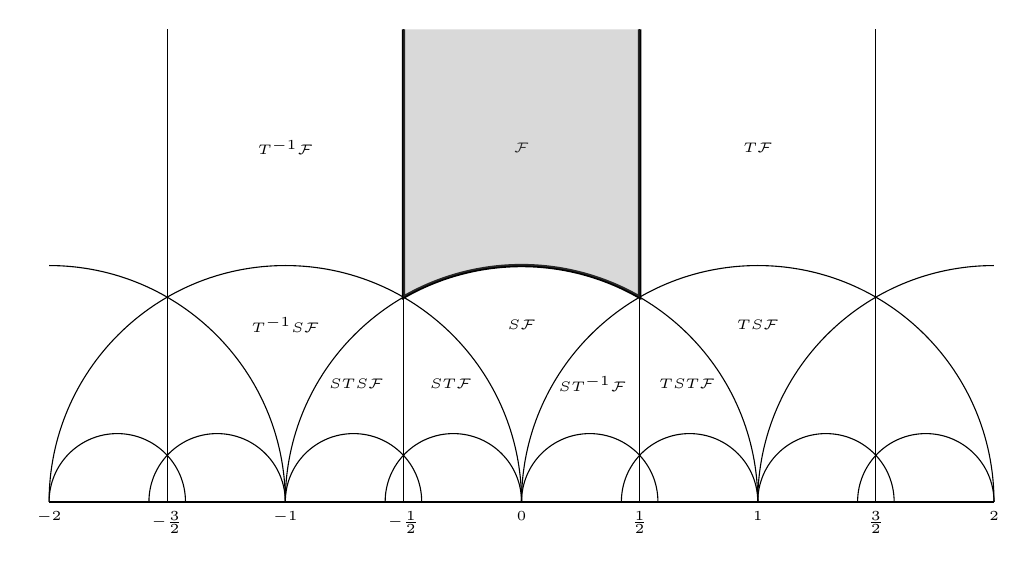
\begin{tikzpicture}[scale=3]
          \def\xmin{-2} \def\xmax{2}
          \def\ymin{0} \def\ymax{2}
          \draw[thick] (\xmin,0) -- (\xmax,0);

          \draw[very thick] (0.5,\ymax) -- (0.5,{sqrt(3)/2}) arc (60:120:1) -- (-0.5,\ymax);

          \node at (-0.5,0) [below] {\tiny{$-\frac{1}{2}$}};
          \node at (0.5,0) [below] {\tiny{$\frac{1}{2}$}};
          \node at (-1.5,0) [below] {\tiny{$-\frac{3}{2}$}};
          \node at (1.5,0) [below] {\tiny{$\frac{3}{2}$}};
          \node at (0,0) [below] {\tiny{$0$}};
          \node at (-1,0) [below] {\tiny{$-1$}};
          \node at (1,0) [below] {\tiny{$1$}};
          \node at (-2,0) [below] {\tiny{$-2$}};
          \node at (2,0) [below] {\tiny{$2$}};

          \draw[thin] (0.5,0) -- (0.5,\ymax);
          \draw[thin] (-0.5,0) -- (-0.5,\ymax);
          \draw[thin] (1.5,0) -- (1.5,\ymax);
          \draw[thin] (-1.5,0) -- (-1.5,\ymax);

          \draw (1,0) arc (0:180:1);
          \draw (-1,0) arc (0:90:1);
          \draw (2,1) arc (90:180:1);

          \draw (0,0) arc (0:180:1);
          \draw (2,0) arc (0:180:1);

          \draw (1,0) arc (0:180:{sqrt(3)/6});
          \draw ({sqrt(3)/3},0) arc (0:180:{sqrt(3)/6});

          \draw (2,0) arc (0:180:{sqrt(3)/6});
          \draw ({1+sqrt(3)/3},0) arc (0:180:{sqrt(3)/6});

          \draw (0,0) arc (0:180:{sqrt(3)/6});
          \draw ({(sqrt(3)/3)-1},0) arc (0:180:{sqrt(3)/6});

          \draw (-1,0) arc (0:180:{sqrt(3)/6});
          \draw ({(sqrt(3)/3)-2},0) arc (0:180:{sqrt(3)/6});

          \node at (0,1.5) {\tiny{$\mc{F}$}};
          \node at (-1,1.5) {\tiny{$T^{-1}\mc{F}$}};
          \node at (1,1.5) {\tiny{$T\mc{F}$}};
          \node at (0,0.75) {\tiny{$S\mc{F}$}};
          \node at (-1,0.75) {\tiny{$T^{-1}S\mc{F}$}};
          \node at (1,0.75) {\tiny{$TS\mc{F}$}};
          \node at (-0.7,0.5) {\tiny{$STS\mc{F}$}};
          \node at (-0.3,0.5) {\tiny{$ST\mc{F}$}};
          \node at (0.3,0.5) {\tiny{$ST^{-1}\mc{F}$}};
          \node at (0.7,0.5) {\tiny{$TST\mc{F}$}};

          \begin{scope}
              \path[clip] (0.5,\ymax) -- (0.5,{sqrt(3)/2}) arc (60:120:1) -- (-0.5,\ymax) -- cycle;
              \fill[gray,opacity=0.3] (-0.5,0) rectangle (0.5,\ymax);
          \end{scope}
        \end{tikzpicture}
        \caption{The fundamental domain of $\PSL_{2}(\Z)\backslash\H$} \label{fig:fundamental_domain_modular_group}
      \end{figure}

      The shaded region in \cref{fig:fundamental_domain_modular_group} is the fundamental domain in \cref{prop:fundamental_domain_modular_group} and we call it the \textbf{standard fundamental domain}\index{standard fundamental domain}. \cref{fig:fundamental_domain_modular_group} also displays how this fundamental domain changes under the actions of the generators of $\PSL_{2}(\Z)$ as in \cref{prop:PSL_generator}. A fundamental domain for any other modular curve can be built from the standard fundamental domain as the following proposition shows (see \cite{kilford2015modular} for a proof):

      \begin{proposition}\label{prop:fundamental_domain_congruence_subgroup}
        Let $\G$ be any congruence subgroup. Then
        \[
          \mc{F}_{\G} = \bigcup_{\g \in \G\backslash\PSL_{2}(\Z)}\g\mc{F},
        \]
        is a fundamental domain for $\G\backslash\H$.
      \end{proposition}

      We might notice that $\mc{F}$ in \cref{fig:fundamental_domain_modular_group} is unbounded as it doesnt contain the point $\infty$. However, if we consider $\mc{F} \cup \{\infty\}$ then it would appear that this space is compact. The point $\infty$ is an example of a cusp and we now make this idea precise. Since any $\g \in \PSL_{2}(\Z)$ preserves $\hat{\R}$ and $\g$ has integer entries, $\g$ also preserves $\Q \cup \{\infty\}$. A \textbf{cusp}\index{cusp} of $\GH$ is an element of of $\G\backslash(\Q \cup \{\infty\})$. As $\G$ has finite index in the modular group, there can only be finitely many cusps and the number of cusps is at most the index of $\G$. In particular, the $\G$-orbit of $\infty$ is a cusp of $\GH$. We denote cusps by representatives of their equivalence classes. For example, we let $\infty$ denote the cusp $\G\infty$.

      \begin{remark}
        It turns out that the cusps can be represented as the points needed to make a fundmantal domain $\mc{F}_{\G}$ compact as a subset of $\hat{\C}$. To see this, suppose $\mf{a}$ is a limit point of $\mc{F}_{\G}$ that does not belong to $\mc{F}_{\G}$. Then $\mf{a} \in \hat{\R}$. In the case of the standard fundmantal domain $\mc{F}$, $\mf{a} = \infty$ which is a cusp. Otherwise, $\mc{F}_{\G}$ is a union of images of $\mc{F}$ by \cref{prop:fundamental_domain_congruence_subgroup} and since $\PSL_{2}(\Z)\infty = \Q \cup \{\infty\}$, we find that $\mf{a} \in \Q \cup \{\infty\}$.
      \end{remark}

      If $\mf{a} = \frac{a}{c}$ with $(a,c) = 1$ is a cusp of $\GH$ not equivaent to $\infty$, then there exists an $\s_{\mf{a}} \in \PSL_{2}(\Z)$ such that $\s_{\mf{a}}\infty = \mf{a}$. Indeed, there exists integers $d$ and $b$ such that $ad-bc = 1$ by B\'ezout's identity and then $\s_{\mf{a}} = \begin{pmatrix} a & b \\ c & d \end{pmatrix}$ is such a matrix. If $\mf{a} = \infty$ then we let $\s_{\mf{a}}$ be the identity matrix. We call $\s_{\mf{a}}$ a \textbf{scaling matrix}\index{scaling matrix} for the cusp $\mf{a}$. Scaling matrices are useful because it allows us to transfer information at the cusp $\mf{a}$ to the cusp at $\infty$ which is usually much easier to analyze. We let $\G_{\mf{a}} \le \G$ denote the stabilizer subgroup of $\mf{a}$. In particular, if $\s_{\mf{a}}$ is a scaling matrix for $\mf{a}$ then $\G_{\mf{a}} = \s_{\mf{a}}\G_{\infty}\s_{\mf{a}}^{-1} \cap \G$. We can actually describe $\G_{\infty}$ explicitly. If $\g = \begin{pmatrix} a & b \\ c & d \end{pmatrix} \in \G$ stabilizes $\infty$, then necessarily $c = 0$ and since $\det(\g) = 1$ we must have $a = d = 1$. Therefore $\g = \begin{pmatrix} 1 & b \\ 0 & 1 \end{pmatrix}$ for some $b \in \Z$ and $\g$ acts on $\H$ by translation by $b$. Letting $t$ be the smallest positive integer such that $\begin{pmatrix} 1 & t \\ 0 & 1 \end{pmatrix} \in \G$, we have $\G_{\infty} = \left\<\begin{pmatrix} 1 & t \\ 0 & 1 \end{pmatrix}\right\>$. If $\G$ is of level $N$, then $N$ is the smallest positive integer such that $\G(N) \le \G$ so that $\begin{pmatrix} 1 & N \\ 0 & 1 \end{pmatrix}$ is the minimal translation guaranteed to belong to $\G$. However, there may be smaller translations so in general $t \le N$.
  \section{The General Setup for Modular Forms}\label{sec:The_General_Setup_for_Modular_Forms}
    \subsection*{Modular Forms}
      Let $\G$ be a congruence subgroup. We say that a function $f:\H \to \C$ is an \textbf{automorphic form}\index{automorphic form} on $\G\backslash\H$ if $f(\g z) = f(z)$ for all $\g \in \G$. That is, $f$ is $\G$-invariant and we call this invariance the \textbf{automorphy condition}\index{automorphy condition}. Modular forms are obtained by relaxing the automorphy condition (and imposing some additional mild conditions). Let $\G$ be a congruence subgroup of level $N$ and let $\e:\G \to \C$ be such that $|\e(\g)| = 1$ for all $\g \in \G$. We say that a function $f:\H \to \C$ is a \textbf{modular form}\index{modular form} of weight $k \in \left(\Z_{\ge 0}+\frac{1}{2}\Z_{\ge 0}\right)-\{0\}$, level $N$, and \textbf{nebentypus}\index{nebentypus} or \textbf{twist}\index{twist} $\e$ on $\GH$ if the following properties are satisfied:
      \begin{enumerate}[label=(\roman*)]
        \item $f$ is holomorphic on $\H$.
        \item $f(\g z) = \e(\g)(cz+d)^{k}f(z)$ for all $\g = \begin{pmatrix} a & b \\ c & d \end{pmatrix} \in \G$.
        \item $f(\a z)$ remains bounded as $\Im(z) \to \infty$ for all $\a \in \PSL_{2}(\Z)$.
      \end{enumerate}
      Condition (ii) is called the \textbf{modularity condition}\index{modularity condition} and we say $f$ is \textbf{modular}\index{modular}. If $\e$ is not trivial, that is $\e(\g) \neq 1$ for some $\g \in \G$, then we say $f$ is \textbf{twisted}\index{twisted} by $\e$. In the case $\e$ is trivial, we say that $f$ is \textbf{untwisted}\index{untwisted}. We set $j(\g,z) = (cz+d)$ and call $j(\g,z)$ the \textbf{factor of modularity}\index{factor of modularity} of $f$. Condition (iii) is called the \textbf{growth condition}\index{growth condition} and we say $f$ is \textbf{holomorphic at the cusps}\index{holomorphic at the cusps}. Also, we say $f$ is a \textbf{cuspform}\index{cuspform} if in addition,
      \begin{enumerate}[label=(\roman*)]
        \setcounter{enumi}{3}
        \item $f(\a z) \to 0$ as $\Im(z) \to \infty$ for all $\a \in \PSL_{2}(\Z)$.
      \end{enumerate}

      Modular forms also admit Fourier series provided that the nebentypus is simple. Suppose that $\e(\g) = 1$ whenever $c = 0$ if $\g = \begin{pmatrix} a & b \\ c & d \end{pmatrix}$. Let $\begin{pmatrix} 1 & t \\ 0 & 1 \end{pmatrix}$ be the smallest translation belonging to $\G$. By modularity,
      \[
        f(z+t) = f\left(\begin{pmatrix} 1 & t \\ 0 & 1 \end{pmatrix}z\right) = f(z).
      \]
      so that $f$ is $t$-periodic.

      \begin{remark}
        If $f$ is $t$-periodic, then we may think of $f$ as a function on $\G_{\infty}\backslash\H$. Taking representatives, $\G_{\infty}\backslash\H$ is a strip in $\H$ with bounded real part so that $f$ is a function on a domain with boudned real part.
      \end{remark}

      As $f$ is $t$-periodic it admits a Fourier series
      \[
        f(z) = \sum_{n \in \Z}a(n,y)e^{\frac{2\pi inx}{t}}.
      \]
      Actually, the Fourier coefficients $a_{\infty}(n,y)$ do not depend on $y$. To see this, since $f$ is holomorphic we know
      \[
        \frac{\del f}{\del\conj{z}} = \frac{1}{2}\left(\frac{\del f}{\del x}+i\frac{\del f}{\del y}\right) = 0.
      \]
      Substiuting in the Fourier series and equating coefficients we obtain the ODE
      \[
        2\pi na(n,y)+a'(n,y) = 0,
      \]
      where the $'$ indicates differentiation with respect to $y$. Solving this ODE (by separation of variables) we see that there exists an $a(n)$ such that
      \[
        a(n,y) = a(n)e^{-2\pi ny}.
      \]
      Using these constant coefficients instead, we say $f$ has a \textbf{Fourier series at the $\infty$ cusp}\index{Fourier series at the $\infty$ cusp}:
      \[
        f(z) = \sum_{n \in \Z}a_{\infty}(n)e^{\frac{2\pi inz}{t}}.
      \]
      Accordingly, we say $f$ is \textbf{holomorphic at infinity}\index{holomorphic at infinity} if
      \[
        \lim_{z \to \infty}\sum_{n \in \Z}a_{\infty}(n)e^{\frac{2\pi inz}{t}},
      \]
      exists and is finite. This is equivalent to $f(z)$ remaining bounded as $\Im(z) \to \infty$ and therefore the Fourier series is actually over all $n \ge 0$ (the negative terms do not exhibit decay as $\Im(z) \to \infty$ unless their Fourier coefficients vanish). Moreover, the limit above is $a_{\infty}(0)$ and $f$ will have exponential decay to $a_{\infty}(0)$ as $\Im(z) \to \infty$. Writing $z = x+iy$ and fixing any $y > 0$, $f$ restricts to a $t$-periodic smooth function on $\R$ that is integrable on $[0,t]$, as it is holomorphic, so we have
      \[
        a_{\infty}(n) = \int_{0}^{t}f_{\infty}(x+iy)e^{-\frac{2\pi inx}{t}}\,dx.
      \]
      For a general cusp $\mf{a}$ of $\GH$, let $\s_{\mf{a}}$ be a scaling matrix for $\mf{a}$. That is, $\s_{\mf{a}}\infty = \mf{a}$. Then $f(\s_{\mf{a}}z)$ is holomorphic at infinity precisely when $f(\s_{\mf{a}}z)$ remains bounded as $\Im(z) \to \infty$ which is to say that $f(z)$ remains bounded as $z \to \mf{a}$. This motivates the saying that $f$ is holomorphic at the cusps. Accordingly, $f$ has a \textbf{Fourier series at the $\mf{a}$ cusp}\index{Fourier series at the $\mf{a}$ cusp}:
      \[
        f(\s_{\mf{a}}z) = \sum_{n \ge 0}a_{\mf{a}}(n)e^{\frac{2\pi inz}{t}}.
      \]
      The Fourier coefficients $a_{\mf{a}}(n)$ are then given by
      \[
        a_{\mf{a}}(n) = \int_{0}^{t}f(\s_{\mf{a}}(x+iy))e^{-\frac{2\pi inx}{t}}\,dx,
      \]
      for any fixed $y > 0$. Notice that $f$ is a cuspform precisely if $a_{\mf{a}}(0) = 0$ for every Fourier series of $f$ at every cusp $\mf{a}$. In particular, $f$ exhibits exponential decay to zero near the cusps. Also, the Fourier series above is independent of the scaling matrix $\s_{\mf{a}}$. To see this, suppose $\s'_{\mf{a}}$ is another scaling matrix. Then $\s'_{\mf{a}} = \s_{\mf{a}}\begin{pmatrix} 1 & mt \\ 0 & 1 \end{pmatrix}$ for some integer $m \ge 1$ because the product $\s_{\mf{a}}^{-1}\s'_{\mf{a}}$ stabilizes $\infty$. By the periodicity of $f$, we then have $f(\s'_{\mf{a}}z) = f(\s_{\mf{a}}z)$. So in particular, we only need to check condition (iii) for a set of scaling matrices for the cusps since every element of $\PSL_{2}(\Z)$ is either a scaling matrix for a cusp or belongs to $\G_{\infty}$ depending on if it fixes $\infty$ or not.
    \subsection*{The Nebentypus \& Cocycles}
      Let $\g,\g' \in \G$ and suppose $j(\g,z)$ is the factor of modularity of a modular form $f$ on $\GH$. Set $\g = \begin{pmatrix} a & b \\ c & d \end{pmatrix}$ and $\g' = \begin{pmatrix} a' & b' \\ c' & d' \end{pmatrix}$ so that $\g'\g = \begin{pmatrix} a'a+b'c & a'b+b'b \\ c'a+d'c & c'b+d'd \end{pmatrix}$. Then
      \begin{align*}
        j(\g',\g z)j(\g,z) &= \left(c'\frac{az+b}{cz+d}+d'\right)(cz+d) \\
        &= \left(c'\frac{az+b}{cz+d}+d'\right)(cz+d) \\
        &= (c'(az+b)+d'(cz+d)) \\
        &= (c'a+d'c)z+c'b+d'd) \\
        &= j(\g'\g,z).
      \end{align*}
      In short,
      \[
        j(\g'\g,z) =  j(\g',\g z)j(\g,z),
      \]
      and this is called the \textbf{cocycle condition}\index{cocycle condition} for $j(\g,z)$. If $f$ is a modular form of weight $k$ and nebentypus $\e$, then modularity of implies
      \[
        \e(\g'\g)j(\g'\g,z)^{k}f(z) = f(\g'\g z) = \e(\g')j(\g',\g z)^{k}f(\g z) = \e(\g')j(\g',\g z)^{k}\e(\g)j(\g,z)^{k}f(z),
      \]
      and by the cocycle condition we conclude $\e(\g'\g) = \e(\g')\e(\g)$ so that $\e$ is a homomorphism. So modularity of $f$ with the cocycle condition implies that the nebentypus is a homomorphism. The cocycle condition also immediately implies that the factor of modularity is determined by any set of generators for $\G$. This is a very useful fact to remember because it is often easier to verify modularity on a generating set of a congruence subgroup.
  \section{The Theory of Modular Forms}
    In practice the primary congruence subgroups of interest are $\G_{1}(N)$ and $\G_{0}(N)$ because these are the congruence subgroups for which we have the theory of Hecke operators. Moreover, these congruence subgroups are such that $\G_{\infty} = \left\<\begin{pmatrix} 1 & 1 \\ 0 & 1 \end{pmatrix}\right\>$ so that all of the modular forms are $1$-periodic. Nevertheless, many of the following results will be stated for more general congruence subgroups so we will always be clear about what properties the implicit congruence subgroup satisfies. However, the level will always be noted as $N$ unless otherwise specified. Moreover, it will be useful to consider modular forms as functions on $\G_{\infty}\backslash\H$ where the domain has bounded real part.
    \subsection*{Twists by Dirichlet Characters}
      Let $\G$ be a congruence subgroup of level $N$. Sometimes we will be interested in modular forms with nontrivial nebentypus on certian congruence subgroups. This twist will be given by a Dirichlet character $\chi$ with conductor $q \mid N$. In particular,
      \[
        \e(\g) = \chi(\g) = \chi(d),
      \]
      where $\g = \begin{pmatrix} a & b \\ c & d \end{pmatrix}$. It turns out that to get modular forms that are not identically zero, the weight $k$ depends on $\chi$. Indeed, if $f$ is a weight $k$ modular form on $\GH$, then by modularity
      \[
        f(z) = f\left(\begin{pmatrix} -1 & 0 \\ 0 & -1 \end{pmatrix}z\right) = \chi(-1)(-1)^{k}f(z),
      \]
      So $f$ is identically zero unless $\chi(-1) = (-1)^{k}$. In other words, if $\chi$ is odd then $k$ must be odd and if $\chi$ is even then $k$ must be even. If $\chi$ is the trival character, then the twist is actually trivial and so modular forms twisted by Dirichlet characters generalize untwisted modular forms.
    \subsection*{Eisenstein \& Poincar\'e Series}
      Let $\G$ be a congruence subgroup of level $N$. We will introduce two important classes of modular forms on $\GH$ namely the Eisenstein series and the Poincar\'e series. For any weight $k \ge 4$ and Dirichlet character $\chi$ with conductor $q \mid N$, we define the \textbf{Eisenstein series}\index{Eisenstein series} $E_{k,\chi}$ of weight $k$ twised by $\chi$ on $\GH$ by
      \[
        E_{k,\chi}(z) = \sum_{\g \in \GG}\cchi(\g)j(\g,z)^{-k},
      \]

      \begin{remark}
        The reason why we restrict to $k \ge 4$ is because for $k = 0$ the modularity condition reduces to $\G$-invariance, which we are not interested in, and for $k = 2$ the Eisenstein series need not converge (see \cref{prop:general_lattice_sum_convergence_for_two_variables}).
      \end{remark}

      Recall that $\G_{\infty} = \left\<\begin{pmatrix} 1 & t \\ 0 & 1 \end{pmatrix}\right\> \cong \Z$ where $t \ge 1$ is the smallest positive integer such that $\begin{pmatrix} 1 & t \\ 0 & 1 \end{pmatrix} \in \G$. Since
      \[
        \begin{pmatrix} 1 & nt \\ 0 & 1 \end{pmatrix}\begin{pmatrix} a & b \\ c & d \end{pmatrix} = \begin{pmatrix} a+ntc & b+ntd \\ c & d \end{pmatrix},
      \]
      each element of $\GG$ corresponds to a unique $(c,d) \in \Z^{2}-\{\mathbf{0}\}$ (some pairs may be excluded depending the congruence subgroup $\G$). Then
      \[
        |E_{k,\chi}(z)| \le \sum_{(c,d) \in \Z^{2}-\{\mathbf{0}\}}\frac{1}{|cz+d|^{k}},
      \]
      and as $k \ge 4$, this latter series converges absolutely uniformly on compacta for $z \in \H$ by \cref{prop:general_lattice_sum_convergence_for_two_variables}. Hence $E_{k,\chi}(z)$ does too and so it is holomorphic on $\H$.

      \begin{remark}\label{rem:Eisenstein_series_on_modular_group}
        In the case of the modular group, a set of representatives for the quotient $\GG$ is
       \[
         \left\{\begin{pmatrix} \ast & \ast \\ c & d \end{pmatrix}:c \ge 0, d \neq 0, (c,d) = 1\right\},
       \]
       because
       \[
         \begin{pmatrix} 1 & n \\ 0 & 1 \end{pmatrix}\begin{pmatrix} a & b \\ c & d \end{pmatrix} = \begin{pmatrix} a+nc & b+nd \\ c & d \end{pmatrix},
       \]
       $ad-bc = 1$ is equivalent to $(c,d) = 1$ by B\'ezout's identity, and we can assume $c \ge 0$ since we are working in $\PSL_{2}(\Z)$. Then $E_{k,\chi}$ is given by
        \[
          E_{k,\chi}(z) = \sum_{\substack{c \ge 0, d \neq 0 \\ (c,d) = 1}}\frac{\cchi(d)}{(cz+d)^{k}} = 1+\sum_{\substack{c \ge 1, d \in \Z \\ (c,d) = 1}}\frac{\cchi(d)}{(cz+d)^{k}}.
        \]
        A full treatment of these series when $\chi$ is the trivial character can be found in \cite{conrad2016modular}.
      \end{remark}

      We now show that $E_{k,\chi}$ is modular. This is just a computation:
      \begin{align*}
        E_{k,\chi}(\g z) &= \sum_{\g' \in \GG}\cchi(\g')j(\g',\g z)^{-k} \\
        &= \sum_{\g' \in \GG}\cchi(\g')\left(\frac{j(\g'\g,z)}{j(\g,z)}\right)^{-k} && \text{cocycle condition} \\
        &= j(\g,z)\sum_{\g' \in \GG}\cchi(\g')j(\g'\g,z)^{-k} \\
        &= \chi(\g)j(\g,z)\sum_{\g' \in \GG}\cchi(\g')\cchi(\g)j(\g'\g,z)^{-k} \\
        &= \chi(\g)j(\g,z)\sum_{\g' \in \GG}\cchi(\g'\g)j(\g'\g,z)^{-k} \\
        &= \chi(\g)j(\g,z)E_{k,\chi}(z),
      \end{align*}
      where the last equality follows since $\g' \to \g'\g^{-1}$ is a bijection on $\G$. To verify holomorphy at the cusps, we will need a technical lemma:

      \begin{lemma}\label{lem:technical_Eisenstein_convergence_lemma}
        Let $a,b > 0$ be real numbers and consider the half-strip
        \[
          S_{a,b} = \{z \in \H:|\Re(z)| \le a, \Im(z) \ge b\}.
        \]
        For any $z \in S_{a,b}$ there is a $\d \in (0,1)$ such that
        \[
          |nz+m| \ge \d|ni+m|,
        \]
        for all $n,m \in \Z$ and all $z \in S_{a,b}$.
      \end{lemma}
      \begin{proof}
        If $n = 0$ then any $\d$ is sufficient and this $\d$ is independent of $z$. If $n \neq 0$, then the desired inequality is equivalent to
        \[
          \left|\frac{z+\frac{m}{n}}{i+\frac{n}{m}}\right| \ge \d.
        \]
        So consider the function
        \[
          f(z,x) = \left|\frac{z+x}{i+x}\right|,
        \]
        for $z \in S_{a,b}$ and real $x$. It suffices to show $f(z,x) \ge \d$. As $z \in \H$, $z-x \neq 0$ so that $f(z,x)$ is continuous and $f(z,x) > 0$ for all $z$ and $x$. Now let $Y > b$ and consider the region
        \[
          S_{a,b}^{Y} = \{z \in \H:|\Re(z)| \le a, b \le \Im(z) \le Y\}.
        \]
        We claim that there exists a $Y$ such that if $\Im(z) > Y$ and $|x| > Y$ then $f(z,x)^{2} > \frac{1}{4}$. Indeed, we compute
        \[
          f(z,x)^{2} = \frac{(z+x)(\conj{z}+x)}{(i+x)(-i+x)} = \frac{|z|^{2}+2\Re(z)x+x^{2}}{1+x^{2}} \ge \frac{\Im(z)+x^{2}}{1+x^{2}},
        \]
        where in the inequality we have used that $|z|^{2} \ge \Im(z)$ and $\Re(z)$ is bounded. Now $\frac{x^{2}}{1+x^{2}} \to 1$ as $x \to \pm\infty$ so choosing $Y$ such that $|x| > Y$ implies $\frac{x^{2}}{1+x^{2}} \ge \frac{1}{4}$ yields
        \[
          \frac{\Im(z)+x^{2}}{1+x^{2}} \ge \frac{\Im(z)}{1+x^{2}}+\frac{x^{2}}{1+x^{2}} \ge \frac{\Im(z)}{1+x^{2}}+\frac{1}{4} > \frac{1}{4}.
        \]
        It follows that $f(z,x) > \frac{1}{2}$ outside of $S_{a,b}^{Y} \x [-Y,Y]$. But this latter region is compact and so $f(z,x)$ obtains a minimum $\d'$ on it. Then set $\d = \min\{\frac{1}{2},\d'\}$ and we are done.
      \end{proof}

      We can now show that $E_{k,\chi}$ is holomorphic at the cusps. Let $\s_{\mf{a}}$ be a scaling matrix for the cusp $\mf{a}$. Since each element of $\GG$ corresponds to a unique $(c,d) \in \Z^{2}-\{\mathbf{0}\}$, we have the bound
      \[
        |E_{k,\chi}(\s_{\mf{a}}z)| \le \sum_{(c,d) \in \Z^{2}-\{\mathbf{0}\}}\frac{1}{|c\s_{\mf{a}}z+d|^{k}}.
      \]
      Now decompose this last sum as
      \[
        \sum_{(c,d) \in \Z^{2}-\{\mathbf{0}\}}\frac{1}{|c\s_{\mf{a}}z+d|^{k}} = \sum_{d \neq 0}\frac{1}{d^{k}}+\sum_{c \neq 0}\sum_{d \in \Z}\frac{1}{|c\s_{\mf{a}}z+d|^{k}} = 2\sum_{d \ge 1}\frac{1}{d^{k}}+2\sum_{c \ge 1}\sum_{d \in \Z}\frac{1}{|c\s_{\mf{a}}z+d|^{k}}.
      \]
      Since the first sum is bounded, it suffices to show that the double sum is bounded as $\Im(z) \to \infty$. To see this, let $\Im(z) \ge 1$ and $\d$ be as in \cref{lem:technical_Eisenstein_convergence_lemma}. Then for any integer $N \ge 1$ we can write
      \begin{align*}
        \sum_{c \ge 1}\sum_{d \in \Z}\frac{1}{|c\s_{\mf{a}}z+d|^{k}} &= \sum_{c+|d| \le N}\frac{1}{|c\s_{\mf{a}}z+d|^{k}}+\sum_{c+|d| > N}\frac{1}{|c\s_{\mf{a}}z+d|^{k}} \\
        &\le \sum_{c+|d| \le N}\frac{1}{|c\s_{\mf{a}}z+d|^{k}}+\sum_{c+|d| > N}\frac{1}{(\d|ci+d|)^{k}} \\
        &\le \sum_{c+|d| \le N}\frac{1}{|c\s_{\mf{a}}z+d|^{k}}+\frac{1}{\d^{k}}\sum_{c+|d| > N}\frac{1}{|ci+d|^{k}}.
      \end{align*}
      Since $\sum_{c \ge 1}\sum_{d \in \Z}\frac{1}{|ci+d|^{k}}$ converges by \cref{prop:general_lattice_sum_convergence_for_two_variables}, the second sum tends to zero as $N \to \infty$. But the first sum is finite and each term tends to a finite value as $\Im(z) \to \infty$. Hence the double sum does too. This proves holomorphy at $\mf{a}$. We collect all of this work as a theorem:

      \begin{theorem}
        Let $k \ge 4$ and $\chi$ be Dirichlet character with conductor $q \mid N$. The Eisenstein series
        \[
          E_{k,\chi}(z) = \sum_{\g \in \GG}\cchi(\g)j(\g,z)^{-k},
        \]
        is a weight $k$ modular form twisted by $\chi$ on $\GH$.
      \end{theorem}

      \begin{remark}
        The intuition behind the construction of the Eisenstein series $E_{k,\chi}$ is that $E_{k,\chi}$ is built by averaging the twist and factor of modularity over $\G$. Actually, this average happens over $\GG$ because $\G_{\infty}$ acts trivially since $j(\g,z) = 1$ if $\g \in \G_{\infty}$ as $\g = \begin{pmatrix} 1 & n \\ 0 & 1 \end{pmatrix}$ for some $n \in \Z$.
      \end{remark}

      Now we will discuss our second class of modular forms. For every $m \ge 1$, weight $k \ge 4$ and Dirichlet character $\chi$ with conductor $q \mid N$, we define the $m$-th \textbf{Poincar\'e series}\index{Poincar\'e series} $P_{m,k,\chi}$ of weight $k$ twisted by $\chi$ on $\GH$ by
      \[
        P_{m,k,\chi}(z) = \sum_{\g \in \GG}\cchi(\g)j(\g,z)^{-k}e^{2\pi im\g z}.
      \]
      Since for such a $\g$, $\g z$ depends on $a$ and $b$ which are not uniquely associated to an element of $\GG$ (unlike $c$ and $d$), we need to check that $P_{m,k,\chi}$ is actually well-defined. This amounts to checking that $e^{2\pi im\g z}$ is independent of the representative $\g$. It is indeed because if $\g'$ represents the same element as $\g$ in $\GG$, then they differ by an element of $\G_{\infty}$ so that
      \[
        \g' = \begin{pmatrix} a+mc & b+md \\ c & d \end{pmatrix},
      \]
      for some $m \in \Z$. Then
      \[
        e^{2\pi im\left(\frac{(a+mc)z+b+md}{cz+d}\right)} = e^{2\pi im\left(\frac{az+b}{cz+d}\right)}e^{2\pi im^{2}} = e^{2\pi im\left(\frac{az+b}{cz+d}\right)},
      \]
      so $P_{m,k,\chi}$ is well-defined. To see that $P_{m,k,\chi}$ is holomorphic on $\H$, first note that $|e^{2\pi im\g z}| = e^{-2\pi m\Im(\g z)} < 1$ for all $\g \in \G$. Then recall that each element of $\GG$ corresponds to a unique $(c,d) \in \Z^{2}-\{\mathbf{0}\}$ so that
      \[
        |P_{m,k,\chi}(z)| \le \sum_{(c,d) \in \Z^{2}-\{\mathbf{0}\}}\frac{1}{|cz+d|^{k}}.
      \]
      As $k \ge 4$, this latter series converges absolutely uniformly on compacta for $z \in \H$ by \cref{prop:general_lattice_sum_convergence_for_two_variables}. Hence $P_{m,k,\chi}(z)$ does too and so it is holomorphic on $\H$.

      \begin{remark}
        In the case of the modular group, a set of representatives for the quotient $\GG$ is
       \[
         \left\{\begin{pmatrix} \ast & \ast \\ c & d \end{pmatrix}:c \ge 0, d \neq 0, (c,d) = 1\right\},
       \]
       as in \cref{rem:Eisenstein_series_on_modular_group}. Then $P_{m,k,\chi}$ is given by
        \[
          P_{m,k,\chi}(z) = \sum_{\substack{c \ge 0, d \neq 0 \\ (c,d) = 1}}\cchi(d)\frac{e^{2\pi im\left(\frac{az+b}{cz+d}\right)}}{(cz+d)^{k}} = e^{2\pi imz}+\sum_{\substack{c \ge 1, d \in \Z \\ (c,d) = 1}}\cchi(d)\frac{e^{2\pi im\left(\frac{az+b}{cz+d}\right)}}{(cz+d)^{k}},
        \]
        where $a$ and $b$ are chosen such that $\det\left(\begin{pmatrix} a & b \\ c & d \end{pmatrix}\right) = 1$. A full discussion of these series when $\chi$ is the trivial character can be found \cite{snowden2016lectures}.
      \end{remark}

      We now show that $P_{m,k,\chi}$ is modular. This is just a computation:
      \begin{align*}
        P_{m,k,\chi}(\g z) &= \sum_{\g' \in \GG}\cchi(\g')j(\g',\g z)^{-k}e^{2\pi im\g'\g z} \\
        &= \sum_{\g' \in \GG}\cchi(\g')\left(\frac{j(\g'\g,z)}{j(\g,z)}\right)^{-k}e^{2\pi im\g'\g z} && \text{cocycle condition} \\
        &= j(\g,z)\sum_{\g' \in \GG}\cchi(\g')j(\g'\g,z)^{-k}e^{2\pi im\g'\g z} \\
        &= \chi(\g)j(\g,z)\sum_{\g' \in \GG}\cchi(\g')\cchi(\g)j(\g'\g,z)^{-k}e^{2\pi im\g'\g z} \\
        &= \chi(\g)j(\g,z)\sum_{\g' \in \GG}\cchi(\g'\g)j(\g'\g,z)^{-k}e^{2\pi im\g'\g z} \\
        &= \chi(\g)j(\g,z)P_{m,k,\chi}(z),
      \end{align*}
      where the last equality follows because $\g' \to \g'\g^{-1}$ is a bijection on $\G$. Hence $P_{m,k,\chi}(z)$ is modular with factor of modularity $j(\g,z)$. To verify holomorphy at the cusps, let $\s_{\mf{a}}$ be a scaling matrix for the cusp $\mf{a}$. First note that $|e^{2\pi im\g\s_{\mf{a}}z}| = e^{-2\pi m\Im(\g\s_{\mf{a}}z)} < 1$. Then since each element of $\GG$ corresponds to a unique $(c,d) \in \Z^{2}-\{\mathbf{0}\}$, we have the bound
      \[
        |P_{m,k,\chi}(\s_{\mf{a}}z)| \le \sum_{(c,d) \in \Z^{2}-\{\mathbf{0}\}}\frac{1}{|c\s_{\mf{a}}z+d|^{k}},
      \]
      and now we can proceed in exactly the same way used to show that $E_{k,\chi}$ was holomorphic at the cusps. We collect all of this work as a theorem:

      \begin{theorem}
        Let $k \ge 4$ and $\chi$ be a Dirichlet character with conductor $q \mid N$. The Poincar\'e series
        \[
          P_{m,k,\chi}(z) = \sum_{\g \in \GG}j(\g,z)^{-1}e^{2\pi im\g z},
        \]
        is a weight $k$ modular form twisted by $\chi$ on $\GH$.
      \end{theorem}
    \subsection*{Spaces of Modular Forms}
      Let $\G$ be a congruence subgroup of level $N$. Clearly modular forms on $\GH$ of a fixed weight $k \ge 4$ and twist $\chi$ are closed under addition and scalar multiplication over $\C$ and therefore form a vector space. Let $\mc{M}_{k}(\GH,\chi)$ denote this space. If $\G_{1}$ and $\G_{2}$ are two congruence subgroups such that $\G_{1} \le \G_{2}$, then we have the inclusion
      \[
        \mc{M}_{k}(\G_{2}\backslash\H) \subseteq \mc{M}_{k}(\G_{1}\backslash\H).
      \]
      So in general, the smaller the congruence subgroup the more modular forms there are. Moreover, we can form the graded ring $\mc{M}(\GH,\chi)$ generated by modular forms of of all weights and twist $\chi$:
      \[
        \mc{M}(\GH,\chi) = \bigop_{k \ge 4}\mc{M}_{k}(\GH,\chi)
      \]
      This is actually an algebra since if we have two modular forms $f$ and $g$ of weights $k$ and $\ell$ and twists $\chi$ and $\psi$ respectively, then $fg$ is a modular form of weight $k\ell$ and twist $\chi\psi$. Moreover, note that cuspforms are closed under all of these operations so we have the corresponding subsapces $\mc{S}_{k}(\GH,\chi)$ and $\mc{S}(\GH,\chi)$ of cuspforms. If $\chi$ is trivial so that the forms are untwisted, we suppress it from the notation.

      We will need a dimensionality result regarding the space of modular forms of a fixed weight. However, we will only require the result for untwised forms. Why this might seem somewhat restrictive, this will encompass dimensionality results for the twisted forms we will be investigating later. The result is that $\mc{M}_{k}(\GH)$ is never too large (see \cite{diamond2005first} for a proof):

      \begin{theorem}\label{thm:modular_forms_space_classification}
        Fix a weight $k \ge 4$. Then $\mc{M}_{k}(\GH)$ is finite dimensional.
      \end{theorem}

      Since $\mc{S}_{k}(\GH)$ is a subspace of $\mc{M}_{k}(\GH)$, \cref{thm:modular_forms_space_classification} implies that $\mc{S}_{k}(\GH)$ is also finite dimensional. Actually, \cite{diamond2005first} gives explicit formulas for the dimensions of $\mc{M}_{k}(\GH)$ and $\mc{S}_{k}(\GH)$ in terms of properties of the modular curve $\GH$ but we will not need this level of detail.
    \subsection*{Double Coset Operators}
      We are ready to introduce a class of general operators, depending upon double cosets, on any congruence subgroup $\G$ of level $N$. We will soon use these operators to define the diamond and Hecke operators. Recall that $j(\g,z) = (cz+d)$, where $\g = \begin{pmatrix} a & b \\ c & d \end{pmatrix} \in \G$, is the factor of modularity. Actually, $j(\g,z)$ makes sense for any $\g \in \GL_{2}^{+}(\Q)$ and we extend it accordingly. Let $\G_{1}$ and $\G_{2}$ be two congruence subgroups (not necessarily of the same level). For $\a \in \GL_{2}^{+}(\Q)$ consider the double coset
      \[
        \G_{1}\a\G_{2} = \{\g_{1}\a\g_{2}:\g_{1} \in \G_{1}, \g_{2} \in \G_{2}\}.
      \]
      Then $\G_{1}$ acts on the set $\G_{1}\a\G_{2}$ by left multiplication so that it decomposes into a disjoin union of orbit spaces. So
      \[
        \G_{1}\a\G_{2} = \bigcup_{\b_{j}}\G_{1}\b_{j},
      \]
      where the union ranges over a set of orbit representatives $\b_{j}$ for $\G_{1}\a\G_{2}$. The general operators we will define will be double coset operators, but in order for them to be well-defined it is necessary that the orbit decomposition above is a finite union. This is indeed the case (see \cite{diamond2005first} for a proof):

      \begin{proposition}\label{prop:double_congruence_subgroup_coset_decomposition_is_finite}
        Let $\a \in \GL_{2}^{+}(\Q)$. Then the orbit decomposition
        \[
          \G_{1}\a\G_{2} = \bigcup_{\b_{j}}\G_{1}\b_{j},
        \]
        with respect to the action of $\G_{1}$ by left multiplication, is a finite union.
      \end{proposition}

      We will now introduce our operators. Fix some congruence subgroup $\G$ and consider $\mc{M}_{k}(\GH)$. Then for $\a \in \GL_{2}^{+}(\Q)$, we define the weight $k$ operator $[\a]_{k}$ on $\mc{M}_{k}(\GH)$ to be the linear operator given by
      \[
        (f[\a]_{k})(z) = (\det(\a))^{k-1}j(\a,z)^{-k}f(\a z),
      \]
      for any $f \in \mc{M}_{k}(\GH)$. Moreover, $[\a]_{k}$ is multiplicative. Indeed, if $\a,\a' \in \GL_{2}^{+}(\Q)$, then
      \begin{align*}
        ((f[\a']_{k})[\a]_{k})(z) &= (\det(\a))^{k-1}j(\a,z)^{-k}(f[\a']_{k})(\a z) \\
        &= (\det(\a'))^{k-1}(\det(\a))^{k-1}j(\a',\a z)^{-k}j(\a,z)^{-k}f(\a'\a z) \\
        &= (\det(\a'\a))^{k-1}j(\a'\a,z)^{-k}f(\a'\a z) && \text{cocycle condition} \\
        &= (f[\a'\a]_{k})(z).
      \end{align*}
      Also, if $\g \in \G$ and we choose the representative with $\det(\g) = 1$, then
      \[
        (f[\g]_{k})(z) = j(\g,z)^{-k}f(\g(z)) = j(\g,z)^{-k}j(\g,z)^{k}f(z) = f(z).
      \]
      This chain of equalities is equivalent to $f$ being modular, so $f \in \mc{M}_{k}(\GH)$ if and only if $f$ is invariant under the $[\g]_{k}$ operator for $\g \in \G$ where we take the representative with positive determinant. Now let $\G_{1}$ and $\G_{2}$ be two congruence subgroups and let $\a \in \GL_{2}^{+}(\Q)$. We define the weight $k$ \textbf{double coset operator}\index{double coset operator} $[\G_{1}\a\G_{2}]_{k}$ on $\mc{M}_{k}(\G_{1}\backslash\H)$ to be the linear operator given by
      \[
        (f[\G_{1}\a\G_{2}]_{k})(z) = \sum_{\b \in \G_{1}\a\G_{2}}(f[\b]_{k})(z) = \sum_{\b \in \G_{1}\a\G_{2}}(\det(\b))^{k-1}j(\b,\g z)^{-k}f(\b\g z) \\
      \]
      for any $f \in \mc{M}_{k}(\G_{1}\backslash\H)$. By \cref{prop:double_congruence_subgroup_coset_decomposition_is_finite} this sum is finite. It remains to check that $f[\G_{1}\a\G_{2}]_{k}$ is well-defined. Indeed, if $\b$ and $\b'$ belong to the same orbit, then $\b'\b^{-1} \in \G_{1}$. But then as $f \in \mc{M}_{k}(\G_{1}\backslash\H)$, is it invariant under the $[\b'\b^{-1}]_{k}$ operator so that
      \[
        (f[\b]_{k})(z) = ((f[\b'\b^{-1}]_{k})[\b]_{k})(z) = (f[\b']_{k})(z),
      \]
      and therefore the $[\G_{1}\a\G_{2}]_{k}$ operator is well-defined. Actually, $[\G_{1}\a\G_{2}]_{k}:\mc{M}_{k}(\G_{1}\backslash\H) \to \mc{M}_{k}(\G_{2}\backslash\H)$. That is, it takes weight $k$ modular forms on $\G_{1}\backslash\H$ to weight $k$ modular forms on $\G_{2}\backslash\H$. To see this suppose $f \in \mc{M}_{k}(\G_{1}\backslash\H)$ and $\g \in \G_{2}$. Then
      \begin{align*}
        (f[\G_{1}\a\G_{2}]_{k})(\g z) &= \sum_{\b \in \G_{1}\a\G_{2}}(\det(\b))^{k-1}j(\b,\g z)^{-k}f(\b\g z) \\
        &= \sum_{\b \in \G_{1}\a\G_{2}}(\det(\b\g))^{k-1}j(\b,\g z)^{-k}f(\b\g z) && \text{$\det(\g) = 1$} \\
        &= \sum_{\b \in \G_{1}\a\G_{2}}(\det(\b\g))^{k-1}\left(\frac{j(\g,z)}{j(\b\g,z)}\right)^{k}f(\b\g z) && \text{cocycle condition} \\
        &= j(\g,z)^{k}\sum_{\b \in \G_{1}\a\G_{2}}(\det(\b\g))^{k-1}j(\b\g,z)^{-k}f(\b\g z) \\
        &= j(\g,z)^{k}\sum_{\b \in \G_{1}\a\G_{2}}(f[\b]_{k})(z) \\
        &= j(\g,z)^{k}(f[\G_{1}\a\G_{2}]_{k})(z),
      \end{align*}
      where the second to last line follows because $\b \to \b\g^{-1}$ is a bijection on $\G_{1}\a\G_{2}$. So $f[\G_{1}\a\G_{2}]_{k}$ is modular. Holomorphy and the growth condition are immediate since the sum is finite by \cref{prop:double_congruence_subgroup_coset_decomposition_is_finite}. Therefore $f[\G_{1}\a\G_{2}]_{k} \in \mc{M}_{k}(\G_{2}\backslash\H)$. Moreover, the double coset operator $[\G_{1}\a\G_{2}]_{k}$ actually preserves the subspace of cuspforms. To see this, let $\s_{\mf{a}}$ be a scaling matrix for the cusp $\mf{a}$ of $\G_{2}\backslash\H$ and let $f \in \mc{S}_{k}(\G_{1}\backslash\H)$. If $\b \in \G_{1}\a\G_{2}$, then $\b\s_{\mf{a}}$ takes $\infty$ to an element of $\Q \cup \{\infty\}$ since $\a \in \GL_{2}^{+}(\Q)$. In other words, $\b\s_{\mf{a}}\infty = \mf{b}$ for some cusp $\mf{b}$ of $\G_{1}\backslash\H$. Now choose an integer $r \ge 1$ such that $r\a \in \GL_{2}^{+}(\Z)$. As a consquence, there exist integers $n,m \ge 1$ such that $rj(\b,\s_{\mf{a}}z) = |n\s_{\mf{a}}z+m|$. Then letting $\Im(z) > 1$ and $\d$ be as in \cref{lem:technical_Eisenstein_convergence_lemma}, we have
      \[
        j(\b,\s_{\mf{a}}z) = \frac{|n\s_{\mf{a}}z+m|}{r} \ge \frac{\d|ni+m|}{r}.
      \]
      This bound implies
      \[
        (f[\G_{1}\a\G_{2}]_{k})(\s_{\mf{a}}z) = \sum_{\b \in \G_{1}\a\G_{2}}(\det(\b))^{k-1}j(\b,\s_{\mf{a}} z)^{-k}f(\b\s_{\mf{a}} z) \le \left(\frac{\d|ni+m|}{r}\right)^{-k}\sum_{\b \in \G_{1}\a\G_{2}}(\det(\b))^{k-1}f(\b\s_{\mf{a}} z)
      \]
      As $f$ is a cuspform, it has exponential decay to zero near the cusps so that the sum on the right hand side tends to zero as $\Im(z) \to \infty$. This shows that $f[\G_{1}\a\G_{2}]_{k}$ is a cuspform too.

      The double coset operators are the most basic types of operators on modular forms. They are the building blocks needed to define the more important dimaond and Hecke operators.
    \subsection*{The Diamond Operators \& Twisted Modular Forms}
      The next operator is a special case of the weight $k$ operator. To define it, we need to consider both the congruence subgroups $\G_{1}(N)$ and $\G_{0}(N)$. Recall that $\G_{1}(N) \le \G_{0}(N)$ and consider the map
      \[
        \G_{0}(N) \to (\Z/N\Z)^{\ast} \qquad \begin{pmatrix} a & b \\ c & d\end{pmatrix} \to d \tmod{N},
      \]
      ($d$ is invertible modulo $N$ since $c \equiv 0 \tmod{N}$ and $ad-bc = 1$). This is a surjective homomorphism and its kernel is exaclty $\G_{1}(N)$ so that $\G_{1}(N)$ is a normal subgroup of $\G_{0}(N)$ and $\G_{0}(N)/\G_{1}(N) \cong (\Z/N\Z)^{\ast}$. Letting $\a = \begin{pmatrix} \ast & \ast \\ 0 & d \end{pmatrix} \in \G_{0}(N)$ and $f \in \mc{M}_{k}(\G_{1}\backslash\H)$, consider $\left(f\left[\G_{1}(N)\a\G_{1}(N)\right]_{k}\right)(z)$. This is only dependent upon the lower-right entry $d$ of $\a$ taken modulo $N$. To see this, since $\G_{1}(N)$ is normal in $\G_{0}(N)$, $\G_{1}(N)\a = \a\G_{1}(N)$ so that $\G_{1}(N)\a\G_{1}(N) = \a\G_{1}(N)$ and hence there is only one representative for the orbit decomposition. Therefore
      \[
        \left(f\left[\G_{1}(N)\a\G_{1}(N)\right]_{k}\right)(z) = \sum_{\b \in \G_{1}(N)\a\G_{1}(N)}(f[\b]_{k})(z) = (f[\a]_{k})(z).
      \]
      This induces an action of $\G_{0}(N)$ on $\mc{M}_{k}(\G_{1}\backslash\H)$ and since $\G_{1}(N)$ acts trivially, this is really an action of $\G_{0}(N)/\G_{1}(N) \cong (\Z/N\Z)^{\ast}$. In other words, we have an induced action that depends only upon the lower-right entry $d$ of $\a$ taken modulo $N$. So for fixed $d$ modulo $N$, we define the \textbf{diamond operator}\index{diamond operator} $\<d\>:\mc{M}_{k}(\G_{1}(N)\backslash\H) \to \mc{M}_{k}(\G_{1}(N)\backslash\H)$ of weight $k$ to be the linear operator given by
      \[
        (\<d\>f)(z) = (f[\a]_{k})(z),
      \]
      for any $\a = \begin{pmatrix} a & b \\ c & d \end{pmatrix} \in \G_{0}(N)$. Our discussion above has already shown that the diamond operators $\<d\>$ are well-defined. Also, since the weight $k$ operator $[\a]_{k}$ is multiplicative and
      \[
        \begin{pmatrix} \ast & \ast \\ 0 & d \end{pmatrix}\begin{pmatrix} \ast & \ast \\ 0 & e \end{pmatrix} \equiv \begin{pmatrix} \ast & \ast \\ 0 & de \end{pmatrix} \tmod{N},
      \]
      the diamond operators are multiplicative. One reason the diamond operators are useful is that they decompose $\mc{M}_{k}(\G_{1}(N)\backslash\H)$ into eigenspaces. For any Dirichlet character $\chi$ modulo $N$, we define the weight $k$ \textbf{$\chi$-eigenspace}\index{$\chi$-eigenspace} $\mc{M}_{k}(N,\chi)$ by
      \[
        \mc{M}_{k}(N,\chi) = \{f \in \mc{M}_{k}(\G_{1}(N)\backslash\H):\<d\>f = \chi(d)f \text{ for all } d \in (\Z/N\Z)^{\ast}\}.
      \]
      If $\g = \begin{pmatrix} a & b \\ c & d \end{pmatrix} \in \G_{0}(N)$ then
      \[
        \<d\>f = j(\g,z)^{-k}f(\g z) = \chi(d)f(z),
      \]
      is equivalent to $f$ being modular of weight $k$ and twisted by $\chi$ on $\G_{0}(N)\backslash\H$. So the diamond operators sieve out the untwised modular forms on $\G_{1}(N)\backslash\H$ that are twisted modular forms on $\G_{0}(N)\backslash\H$. In particular, $\mc{M}_{k}(N,\chi) = \mc{M}_{k}(\G_{0}(N),\chi)$. As mentioned, these are all of the possible weight $k$ modular forms on $\G_{1}(N)$ (see \cite{diamond2005first} for a proof):

      \begin{proposition}\label{thm:diamond_operator_decomposition}
        Fix a weight $k \ge 4$. Then
        \[
          \mc{M}_{k}(\G_{1}(N)\backslash\H) = \bigop_{\chi}\mc{M}_{k}(N,\chi) = \bigop_{\chi}\mc{M}_{k}(\G_{0}(N)\backslash\H,\chi),
        \]
          where the direct sum ranges over all Dirichlet characters $\chi$ modulo $N$.
      \end{proposition}

      Since $\G_{1}(N) \le \G_{0}(N)$ (actually a normal subgroup), we have that $\mc{M}_{k}(\G_{0}(N)\backslash\H) \subseteq \mc{M}_{k}(\G_{1}(N)\backslash\H)$. So what \cref{thm:diamond_operator_decomposition} is saying is that any untwisted modular form on $\G_{1}(N)\backslash\H$ arises from a modular form twisted by a Dirichlet character on $\G_{0}(N)\backslash\H$. This is a good reason as to why we consider modular forms twisted by Dirichlet characters. They naturally arise in the study of untwisted modular forms.
    \subsection*{Hecke Operators}
      The Hecke operators are special linear operators on spaces of modular forms. Devloping the theory is slightly awkward because it cannot be done in general from the outset. To make the theory easier to parse, we will describe the outline now. First we define the Hecke operators for primes $p$ on the congruence subgroup $\G_{1}(N)$. Then we find an alternaive description for them that does not depend upon $\G_{1}(N)$. Using this alternative description, we lift the Hecke operators for a prime $p$ to any congruence subgroup $\G$. Then we define Hecke operators for any integer $n \ge 1$ on any congruence subgroup. Throughout this discussion, we will obtain corresponding results for modular forms twisted by a Dirichlet character $\chi$ on $\G_{0}(N)\backslash\H$ by \cref{thm:diamond_operator_decomposition}.

      Let's begin. For a prime $p$, we define the $p$-th \textbf{Hecke operator}\index{Hecke operator} $T_{p}:\mc{M}_{k}(\G_{1}(N)\backslash\H) \to \mc{M}_{k}(\G_{1}(N)\backslash\H)$ of weight $k$ to be the linear operator given by
      \[
        (T_{p}f)(z) = \left(\left[\G_{1}(N)\begin{pmatrix} 1 & 0 \\ 0 & p \end{pmatrix}\G_{1}(N)\right]_{k}f\right)(z).
      \]
      Since there is a $p$-th Hecke operator for each weight $k$, if the weight of a modular form is given it is assumed that $T_{p}$ is the Hecke operator corresponding to modular forms of that weight. An explicit desiction of the right coset representatives of $\G_{1}(N)\begin{pmatrix} 1 & 0 \\ 0 & p \end{pmatrix}\G_{1}(N)$ will give an explicit desction of the Hecke operator $T_{p}$. Indeed we have the following proposition (see \cite{diamond2005first} for a proof):

      \begin{proposition}\label{prop:explicit_description_of_Hecke_operators}
        Let $f \in \mc{M}_{k}(\G_{1}(N)\backslash\H)$. Then the Hecke operator $T_{p}$ acts on $f$ as follows:
        \[
          (T_{p}f)(z) = \begin{cases} \displaystyle\sum_{1 \le j \le p-1}\left(f\left[\begin{pmatrix} 1 & j \\ 0 & p \end{pmatrix}\right]_{k}\right)(z) & \text{if $p \mid N$}, \\ \displaystyle\sum_{1 \le j \le p-1}\left(f\left[\begin{pmatrix} 1 & j \\ 0 & p \end{pmatrix}\right]_{k}\right)(z)+\left(f\left[\begin{pmatrix} m & n \\ N & p \end{pmatrix}\begin{pmatrix} 1 & j \\ 0 & p \end{pmatrix}\right]_{k}\right)(z) & \text{if $p \nmid N$}, \end{cases}
        \]
        where $m$ and $n$ are chosen such that $\det\left(\begin{pmatrix} m & n \\ N & p \end{pmatrix}\right) = 1$.
      \end{proposition}

      Notice that the formula for $T_{p}f$ in \cref{prop:explicit_description_of_Hecke_operators} is independent of the congruence subgroup $\G_{1}(N)$ and only dependent on the level $N$. This lets us lift the Hecke operators to any congruence subgroup. If $\G$ is a congruence subgroup of level $N$, then we define the $p$-th \textbf{Hecke operator}\index{Hecke operator} $T_{p}:\mc{M}_{k}(\GH) \to \mc{M}_{k}(\GH)$ of weight $k$ to be the linear operator given by
      \[
        (T_{p}f)(z) = \begin{cases} \displaystyle\sum_{1 \le j \le p-1}\left(f\left[\begin{pmatrix} 1 & j \\ 0 & p \end{pmatrix}\right]_{k}\right)(z) & \text{if $p \mid N$}, \\ \displaystyle\sum_{1 \le j \le p-1}\left(f\left[\begin{pmatrix} 1 & j \\ 0 & p \end{pmatrix}\right]_{k}\right)(z)+\left(f\left[\begin{pmatrix} m & n \\ N & p \end{pmatrix}\begin{pmatrix} 1 & j \\ 0 & p \end{pmatrix}\right]_{k}\right)(z) & \text{if $p \nmid N$}, \end{cases}
      \]
      where $m$ and $n$ are chosen such that $\det\left(\begin{pmatrix} m & n \\ N & p \end{pmatrix}\right) = 1$. This explicit definition of $T_{p}$ can be used to compute how the Hecke operator acts on the Fourier coefficients of a modular form. We have the following explicit result (see \cite{diamond2005first} for a proof when $\G = \G_{1}(N)$ but the same argument works in general):

      \begin{proposition}\label{prop:prime_Hecke_operators_acting_on_Fourier_coefficients}
        Let $f \in \mc{M}_{k}(\GH)$ with Fourier coefficients $a_{\infty}(n)$ at the $\infty$ cusp. Then
        \[
          (T_{p}f)(z) = \sum_{n \ge 0}\left(a_{\infty}(np)+\chi_{N,0}(p)p^{k-1}a_{\infty}\left(\frac{n}{p}\right)\right)e^{2\pi inz},
        \]
        is the Fourier series of $T_{p}f$ at the $\infty$ cusp where it is understood that $a_{\infty}\left(\frac{n}{p}\right) = 0$ if $p \nmid n$.
      \end{proposition}

      We now mention the crucial result about Hecke operators which is that they form a simultaneously commuting family with the diamond operators (see \cite{diamond2005first} for a proof when $\G = \G_{1}(N)$ but the same argument works in general):

      \begin{proposition}\label{prop:Hecke_operators_commute}
        Let $p$ and $q$ be distinct primes and $d \in (\Z/N\Z)^{\ast}$. Then the Hecke operators $T_{p}$ and $T_{q}$ and diamond operators $\<d\>$ simultaneously commute:
        \[
          T_{p}T_{q} = T_{q}T_{p} \quad \text{and} \quad \<d\>T_{p} = T_{p}\<d\>.
        \]
      \end{proposition}

      Of course, the diamond operators are not defined on congruence subgroups other than $\G_{1}(N)$, so when the congruence subgroup is not $\G_{1}(N)$, \cref{prop:Hecke_operators_commute} is understood to mean that the Hecke operators there commute. We can use \cref{prop:Hecke_operators_commute} to construct diamond operators $\<m\>$ and Hecke operators $T_{m}$ for all $m \ge 1$. The \textbf{diamond operator}\index{diamond operator} $\<m\>:\mc{M}_{k}(\G_{1}(N)\backslash\H) \to \mc{M}_{k}(\G_{1}(N)\backslash\H)$ of weight $k$ is determined by the diamond operator $m \tmod{N}$ of weight $k$ if $(m,N) = 1$ and defined to be $\<m\> = 0$, the zero operator, otherwise. Now for the Hecke operators. If $m = p_{1}^{e_{1}}p_{2}^{e_{2}} \cdots p_{k}^{E_{k,\chi}}$ is the prime decomposition of $m$, then we define the $m$-th Hecke operator $T_{m}:\mc{M}_{k}(\GH) \to \mc{M}_{k}(\GH)$ of weight $k$ to be the linear operator given by
      \[
        T_{m} = \prod_{1 \le i \le k}T_{p_{i}^{e_{i}}},
      \]
      where $T_{p^{e}}$ is defined inductively by
      \[
        T_{p^{e}} = T_{p}T_{p^{e-1}}-p^{k-1}T_{p^{e-2}},
      \]
      for all $e \ge 2$. Then by \cref{prop:Hecke_operators_commute}, the Hecke operators $T_{m}$ are multiplicative but not completely multiplicative in $m$. Moreover, they commute with the diamond operators $\<m\>$ when the congruence subgroup is $\G_{1}(N)$. Using these definitions, \cref{prop:prime_Hecke_operators_acting_on_Fourier_coefficients}, and \cref{prop:Hecke_operators_commute}, a more general formula for how the Hecke operators $T_{m}$ act on Fourier coefficients can be derived (see \cite{diamond2005first} for a proof when $\G = \G_{1}(N)$ but the same argument works in general):

      \begin{proposition}\label{prop:general_Hecke_operators_acting_on_Fourier_coefficients}
        Let $f \in \mc{M}_{k}(\GH)$ with Fourier coefficients $a_{\infty}(n)$ at the $\infty$ cusp. Then
        \[
          (T_{m}f)(z) = \sum_{n \ge 0}\left(\sum_{d \mid (n,m)}d^{k-1}a_{\infty}\left(\frac{nm}{d^{2}}\right)\right)e^{2\pi inz},
        \]
        is the Fourier series of $T_{m}f$ at the $\infty$ cusp.
      \end{proposition}
    \subsection*{The Petersson Inner Product}
      Let $\G$ be a congruence subgroup of level $N$ and let $\chi$ be a Dirichlet character with conductor $q \mid N$. We would like to turn $\mc{M}_{k}(\GH,\chi)$ into an inner product space in order to devlope a spectral theory of the linear operators just introduced. Unfortunately this is not possible unless we restrict to $\mc{S}_{k}(\GH,\chi)$. However, we can define the inner product on $\mc{S}_{k}(\GH,\chi) \x \mc{M}_{k}(\GH,\chi)$. Set $V_{\G} = [\PSL_{2}(\Z):\G]$ and recall that this is finite because $\G$ is a congruence subgroup. For $f \in \mc{S}_{k}(\GH,\chi)$ and $g \in \mc{M}_{k}(\GH,\chi)$, define their \textbf{Petersson inner product}\index{Petersson inner product} by
      \[
        \<f,g\> = \frac{1}{V_{\G}}\int_{\mc{F}_{\G}}f(z)\conj{g(z)}\Im(z)^{k}\,d\mu,
      \]
      where $\mc{F}_{\G}$ is a fundamental domain for $\GH$. Since the integrand is $\G$-invariant, the integral is independent of the choice of fundamental domain. The integral is also absolutely bounded by \cref{met:decay_compacta_integral} (since $f$ is a cuspform). These two facts together imply that the Petersson inner product is well-defined. Actually, we have the following proposition:

      \begin{proposition}\label{prop:Petersson_inner_product_hermitian}
        The Petersson inner product is a Hermitian inner product on $\mc{S}_{k}(\GH,\chi)$. Moreover, $\mc{S}_{k}(\GH,\chi)$ is a Hilbert space with respect to this inner product.
      \end{proposition}
      \begin{proof}
        Let $f,g,h \in \mc{S}_{k}(\GH,\chi)$ and $\a \in \C$. Linearity of the integral implies immediately that the Petersson inner product is linear on $\mc{S}_{k}(\GH,\chi)$. It is also positive definite since
        \[
          \<f,f\> = \frac{1}{V_{\G}}\int_{\mc{F}_{\G}}f(z)\conj{f(z)}\Im(z)^{k}\,d\mu = \frac{1}{V_{\G}}\int_{\mc{F}_{\G}}|f(z)|^{2}\Im(z)^{k}\,d\mu \ge 0,
        \]
        with equality if and only if $f$ is identically zero because $|f(z)|^{2}\Im(z)^{k} \ge 0$. To see that it is conjugate symetric, observe
        \begin{align*}
          \conj{\<g,f\>} &= \conj{\frac{1}{V_{\G}}\int_{\mc{F}_{\G}}g(z)\conj{f(z)}\Im(z)^{k}\,d\mu} \\
          &= \frac{1}{V_{\G}}\int_{\mc{F}_{\G}}\conj{g(z)\conj{f(z)}\Im(z)^{k}\,d\mu} \\
          &= \frac{1}{V_{\G}}\int_{\mc{F}_{\G}}\conj{g(z)}f(z)\Im(z)^{k}\,\conj{d\mu} \\
          &= \frac{1}{V_{\G}}\int_{\mc{F}_{\G}}\conj{g(z)}f(z)\Im(z)^{k}\,d\mu \\
          &= \frac{1}{V_{\G}}\int_{\mc{F}_{\G}}f(z)\conj{g(z)}\Im(z)^{k}\,d\mu \\
          &= \<f,g\>,
        \end{align*}
        where the second to last line follows because $d\mu = \frac{dx\,dy}{y^{2}}$. This completes the verification that the Petersson inner product is a Hermitian inner product on $\mc{S}_{k}(\GH,\chi)$. Lastly, since $\mc{S}_{k}(\GH,\chi)$ is finite dimensional it follows immediately that $\mc{S}_{k}(\GH,\chi)$ is also a Hilbert space.
      \end{proof}

      \begin{remark}\label{rem:nondegeneracy_of_Petersson_inner_product}
        As a consquence of \cref{prop:Petersson_inner_product_hermitian}, the Petersson inner product is also nondegenerate on $\mc{S}_{k}(\GH,\chi)$. Actually, for the exact same reasoning this holds on $\mc{S}_{k}(\GH,\chi) \x \mc{M}_{k}(\GH,\chi)$ wherever the Petersson inner product is defined.
      \end{remark}

      Now suppose $f \in \mc{S}_{k}(\GH,\chi)$ with Fouier coefficients $a_{\infty}(n)$ at the $\infty$ cusp. Define linear functionals $\phi_{m,k}:\mc{S}_{k}(\GH,\chi) \to \C$, for every $m \ge 1$, by
      \[
        \phi_{m,k}(f) = a_{\infty}(m).
      \]
      Since $\mc{S}_{k}(\GH,\chi)$ is a finite dimensional Hilbert space, the Riesz representation theorem implies that there exists a unique $v_{m,k} \in \mc{S}_{k}(\GH,\chi)$ such that
      \[
        \<f,v_{m,k}\> = \phi_{m,k}(f) = a_{\infty}(m).
      \]
      We would like to know what these cuspforms are. It turns out that $v_{m,k}$ will be the Poincar\'e series $P_{m,k}$ up to a normalization factor. To see this, we compute the inner product:
      \begin{align*}
        \<f,P_{m,k}\> &= \frac{1}{V_{\G}}\int_{\mc{F}_{\G}}f(z)\conj{P_{m,k}(z)}\Im(z)^{k}\,d\mu \\
        &= \frac{1}{V_{\G}}\int_{\mc{F}_{\G}}f(z)\sum_{\g \in \GG}\chi(\g)\conj{j(\g,z)^{-k}}e^{-2\pi im\conj{\g z}}\Im(z)^{k}\,d\mu \\
        &= \frac{1}{V_{\G}}\int_{\mc{F}_{\G}}f(z)\sum_{\g \in \GG}\frac{\chi(\g)j(\g,z)^{k}}{|j(\g,z)|^{2k}}e^{-2\pi im\conj{\g z}}\Im(z)^{k}\,d\mu \\
        &= \frac{1}{V_{\G}}\int_{\mc{F}_{\G}}f(\g z)\sum_{\g \in \GG}\frac{1}{|j(\g,z)^{k}|^{2k}}e^{-2\pi im\conj{\g z}}\Im(z)^{k}\,d\mu && \text{modularity} \\
        &= \frac{1}{V_{\G}}\int_{\mc{F}_{\G}}f(\g z)\sum_{\g \in \GG}e^{-2\pi im\conj{\g z}}\Im(\g z)^{k}\,d\mu && \text{$\Im(\g z)^{k} = \frac{\Im(z)^{k}}{|j(\g,z)|^{2k}}$.}
      \end{align*}
      Now we put this last integral into a different form. The idea is to rewrite the integral over the fundamental domain $\mc{F}_{\G}$ as an integral over the strip $\G_{\infty}\backslash\H$. First, observe
      \begin{align*}
        \frac{1}{V_{\G}}\int_{\mc{F}_{\G}}f(\g z)\sum_{\g \in \GG}e^{-2\pi im\conj{\g z}}\Im(\g z)^{k}\,d\mu &= \frac{1}{V_{\G}}\int_{\mc{F}_{\G}}\sum_{\g \in \GG}f(\g z)e^{-2\pi im\conj{\g z}}\Im(\g z)^{k}\,d\mu \\
        &= \frac{1}{V_{\G}}\sum_{\g \in \GG}\int_{\mc{F}_{\G}}f(\g z)e^{-2\pi im\conj{\g z}}\Im(\g z)^{k}\,d\mu && \text{DCT} \\
        &= \frac{1}{V_{\G}}\sum_{\g \in \GG}\int_{\g\mc{F}_{\G}}f(z)e^{-2\pi im\conj{z}}\Im(z)^{k}\,d\mu && \text{$z \to \g^{-1}z$.}
      \end{align*}
      Now $\H = \bigcup_{\g \in \G}\g\mc{F}_{\G}$ so that
      \[
        \G_{\infty}\backslash\H = \bigcup_{\g \in \GG}\g\mc{F}_{\G}.
      \]
      Then we can rewrite the integral over the region on the left-hand side to obtain
      \[
        \frac{1}{V_{\G}}\sum_{\g \in \GG}\int_{\g\mc{F}_{\G}}f(z)e^{-2\pi im\conj{z}}\Im(z)^{k}\,d\mu = \frac{1}{V_{\G}}\int_{\G_{\infty}\backslash\H}f(z)e^{-2\pi im\conj{z}}\Im(z)^{k}\,d\mu.
      \]
      The rest is a computation:
      \begin{align*}
        \frac{1}{V_{\G}}\sum_{\g \in \GG}\int_{\g\mc{F}_{\G}}f(z)e^{-2\pi im\conj{z}}\Im(z)^{k}\,d\mu &= \frac{1}{V_{\G}}\int_{\G_{\infty}\backslash\H}f(z)e^{-2\pi im\conj{z}}\Im(z)^{k}\,d\mu \\
        &= \frac{1}{V_{\G}}\int_{0}^{\infty}\int_{0}^{1}\sum_{n \ge 1}a_{\infty}(n)e^{2\pi i(n-m)x}e^{-2\pi(n+m)y}y^{k}\,\frac{dx\,dy}{y^{2}} \\
        &= \frac{1}{V_{\G}}\int_{0}^{\infty}\sum_{n \ge 1}\int_{0}^{1}a_{\infty}(n)e^{2\pi i(n-m)x}e^{-2\pi(n+m)y}y^{k}\,\frac{dx\,dy}{y^{2}} && \text{DCT} \\
        &= \frac{1}{V_{\G}}\int_{0}^{\infty}a_{\infty}(m)e^{-4\pi my}y^{k}\,\frac{dy}{y^{2}},
      \end{align*}
      where the last line follows because
      \begin{equation}\label{equ:Dirac_integral_representation}
        \int_{0}^{1}e^{2\pi i(n-m)x}\,dx = \d_{n-m,0},
      \end{equation}
      so that the inner integral cuts off all the terms except for the $n = m$ term. Then
      \begin{align*}
        \frac{1}{V_{\G}}\int_{0}^{\infty}a_{\infty}(m)e^{-4\pi my}y^{k}\,\frac{dy}{y^{2}} &= \frac{a_{\infty}(m)}{V_{\G}}\int_{0}^{\infty}e^{-4\pi my}y^{k-1}\,\frac{dy}{y} \\
        &= \frac{a_{\infty}(m)}{V_{\G}}\int_{0}^{\infty}e^{-4\pi my}y^{k-1}\,\frac{dy}{y} && \text{$y \to \frac{y}{4\pi m}$} \\
        &= \frac{a_{\infty}(m)}{V_{\G}(4\pi m)^{k-1}}\int_{0}^{\infty}e^{-y}y^{k-1}\,\frac{dy}{y} \\
        &= \frac{\G(k-1)}{V_{\G}(4\pi m)^{k-1}}a_{\infty}(m) && \text{definition of $\G(k-1)$.}
      \end{align*}
      In conclusion,
      \begin{equation}\label{equ:Petersson_inner_product_with_Poincare_series}
        \<f,P_{m,k}\> = \frac{\G(k-1)}{V_{\G}(4\pi m)^{k-1}}a_{\infty}(m).
      \end{equation}
      Now set $\wtilde{P_{m,k}} = \frac{V_{\G}(4\pi m)^{k-1}}{\G(k-1)}P_{m,k}$. For all cuspforms (actually any modular form where the Petersson inner product is defined) $f$,
      \[
        \<f,\wtilde{P_{m,k}}-v_{m,k}\> = 0.
      \]
      By \cref{rem:nondegeneracy_of_Petersson_inner_product}, we conclude $v_{m,k} = \wtilde{P_{m,k}}$. In particular, this shows that the Poincar\'e series $P_{m,k}$ are cuspforms. We usually work with the Poincar\'e series $P_{m,k}$ instead of their normalized counterparts $\wtilde{P_{m,k}}$. In any case, with \cref{equ:Petersson_inner_product_with_Poincare_series} in hand we can prove the following result:

      \begin{theorem}
        The Poincar\'e series span $\mc{S}_{k}(\GH,\chi)$.
      \end{theorem}
      \begin{proof}
        Let $f \in \mc{S}_{k}(\GH,\chi)$ with Fourier coefficients $a_{\infty}(n)$ at the $\infty$ cusp. Since $\G(k-1) \neq 0$, \cref{equ:Petersson_inner_product_with_Poincare_series} implies $\<f,P_{m,k}\> = 0$ if and only if $a_{\infty}(m) = 0$. So $f$ is orthogonal to all the Poincar\'e series if and only if every Fourier coefficient $a_{\infty}(m)$ is zero. But this happens if and only if $f$ is identically zero.
      \end{proof}

      Let's return to the previous computation for a breif moment. The procedure of changing an integral over a fundamental domain $\mc{F}_{\G}$ into an integral over the strip $\G_{\infty}\backslash\H$, or vice versa, works in a more general setting and is called \textbf{unfolding the integral}\index{unfolding the integral} or \textbf{folding the integral}\index{folding the integral} respectively:

      \begin{method}[Unfolding/folding the integral]
        Suppose $\G$ is any congruence subgroup with fundamental domain $\mc{F}_{\G}$, and we are given an absolutely convergent integral of the form
        \[
          \int_{\mc{F}_{\G}}\sum_{\g \in \G'\backslash\G}f(\g z)\,d\mu,
        \]
        where $\G' \le \G$ is a subgroup ($f$ is not necessarily a modular form). Then the above integral can be written in the form
        \[
          \int_{\G'\backslash\H}f(z)\,d\mu.
        \]
        To do this use the dominated convergence theorem to interchange the sum and integral and then make the change of variales $z \to \g^{-1}z$ to put the integral in the form
        \[
          \sum_{\g \in \G'\backslash\G}\int_{\g\F_{\G}}f(z)\,d\mu.
        \]
        Then observe $\H = \bigcup_{\g \in \G}\g\mc{F}_{\G}$ so that $\G'\backslash\H = \bigcup_{\g \in \G'\backslash\G}\g\mc{F}_{\G}$ and the desired result follows. Of course, this is an equality everywhere so we can also run the procedure in reverse.
      \end{method}

      Returning to the Petersson inner product, we restrict to the case when the congruence subgroup is $\G_{1}(N)$. In this instance, the Petersson inner product behaves well with the Hecke operators (see \cite{lang2012introduction} for a proof):

      \begin{proposition}\label{prop:Hecke_operators_self-adjoint}
        On $\mc{S}_{k}(\G_{1}(N))$, the diamond operators $\<m\>$ and Hecke operators $T_{m}$ are normal for all $m \ge 1$ with $(m,N) = 1$.
      \end{proposition}

      In the case of the modular group (the only congreunce subgroup of level $1$), \cref{prop:Hecke_operators_self-adjoint} says that all of the Hecke operators are normal.

      Now suppose $f$ is a nonconstant modular form with Fourier coefficients $a_{\infty}(n)$ at the $\infty$ cusp. If $f$ is such that $T_{m}f = \l_{m}f$ for some $\l_{m} \in \C$, we say $f$ is an \textbf{eigenfunction}\index{eigenfunction} for $T_{m}$ with eigenvalue $\l_{m}$. If $f$ is a modular form on $\G_{1}(N)\backslash\H$ that is a simultaneous eigenfunction for all dimaond operators $\<m\>$ and Hecke operators $T_{m}$ with $(m,N) = 1$, we call $f$ an \textbf{eigenform}\index{eigenform} for $\G_{1}(N)\backslash\H$. In this case \cref{prop:general_Hecke_operators_acting_on_Fourier_coefficients} implies immeditely that the first Fourier coefficient of $T_{m}f$ is $a_{\infty}(m)$ so we must have $a_{\infty}(m) = \l_{m}a_{\infty}(1)$ for all $m \ge 1$ such that $(m,N) = 1$. Therefore we cannot have $a_{\infty}(1) = 0$ for this would mean $f$ is constant. Then we may divide by $a_{\infty}(1)$ to force $a_{\infty}(1) = 1$. It follows that the Fourier coefficients of $f$, relative to the level $N$, are precisely the eigenvalues of $f$. In this case we say $f$ is \textbf{normalized}\index{normalized}. The spectral theorem along with \cref{prop:Hecke_operators_commute,prop:Hecke_operators_self-adjoint} together give the following result:

      \begin{theorem}\label{thm:eigenforms_forms_spectral_theory}
        $\mc{S}_{k}(\G_{1}(N)\backslash\H)$ admits an orthonormal basis of eigenforms with respect to the Petersson inner product.
      \end{theorem}

      Putting \cref{prop:Hecke_operators_commute} together with our definition of $T_{m}$ implies that the Fourier coefficients of $f$ at the $\infty$ cusp that are relatively prime to the level $N$ are multiplicative and satisfy the recursion
      \begin{equation}\label{equ:eigenform_Fourier_coefficient_recursion}
        a_{\infty}(p^{e}) = a_{\infty}(p^{e-1})a_{\infty}(p)-p^{k-1}a_{\infty}(p^{e-2}),
      \end{equation}
      for primes $p$, integers $e \ge 2$, and where $k$ is the weight of $f$.
  \section{The General Setup for Maass Forms}
    \subsection*{Maass Forms}
      Maass forms are the $\G$-invariant analogous to modular forms. We start with the Laplace operator. The \textbf{Laplace operator}\index{Laplace operator} on $\H$ is the linear operator $\D$ on holomorphic functions on $\H$ given by
      \[
        \D = -y^{2}\left(\frac{\del^{2}}{\del x^{2}}+\frac{\del^{2}}{\del y^{2}}\right).
      \]
      This operator behaves well with respect to the $\PSL_{2}(\Z)$ action on $\H$ as the following proposition shows (see \cite{motohashi1997spectral} for a proof):

      \begin{proposition}\label{prop:Laplace_is_invariant}
        The Laplace operator $\D$ is $\PSL_{2}(\Z)$-invariant. That is, if $f$ is a holomorphic function on $\H$ and $\g \in \PSL_{2}(\Z)$, then
        \[
          \D(f(\g z)) = (\D f)(\g z).
        \]
      \end{proposition}

      Let $\G$ be a congruence subgroup and notice that \cref{prop:Laplace_is_invariant} implies that the Laplace operator is $\G$-invariant. We are now ready to introduce and investigate Maass forms. They are special functions that are also eigenfunctions for the Laplace operator. We say that a function $f:\H \to \C$ is a \textbf{Maass form}\index{Maass form} on $\GH$ with eigenvalue $\l$ if the following properties are satisfied:
      \begin{enumerate}[label=(\roman*)]
        \item $f$ is smooth on $\H$.
        \item $f$ is an automorphic form on $\GH$.
        \item $f$ is an eigenfunction for $\D$ with eigenvalue $\l$.
        \item $f(\a z) = o(e^{2\pi\Im(z)})$ as $\Im(z) \to \infty$ for all $\a \in \PSL_{2}(\Z)$.
      \end{enumerate}
      Condition (iv) is called the \textbf{growth condition}\index{growth condition} for $f$ and we say $f$ is of \textbf{moderate growth at the cusps}\index{moderate growth at the cusps}. Now let $\begin{pmatrix} 1 & t \\ 0 & 1 \end{pmatrix}$ be the smallest translation belonging to $\G$ so that $\G_{\infty}$. Since $f$ is $\G$-invariant
      \[
        f(z+t) = f\left(\begin{pmatrix} 1 & t \\ 0 & 1 \end{pmatrix}z\right) = f(z).
      \]
      so that $f$ is $t$-periodic.

      \begin{remark}
        If $f$ is $t$-periodic, then we may think of $f$ as a function on $\G_{\infty}\backslash\H$. Taking representatives, $\G_{\infty}\backslash\H$ is a strip in $\H$ with bounded real part so that $f$ is a function on a domain with boudned real part.
      \end{remark}

      Then exactly as for modular forms, if $\mf{a}$ is a cusp of $\GH$ and $\s_{\mf{a}}$ is a scaling matrix for $\mf{a}$, $f$ has a \textbf{Fourier series at the $\mf{a}$ cusp}\index{Fourier series at the $\mf{a}$ cusp}:
      \[
        f(\s_{\mf{a}}z) = \sum_{n \in \Z}a_{\mf{a}}(n,y)e^{\frac{2\pi inx}{t}},
      \]
      where this chain of equalities is independent of the scaling matrix $\s_{\mf{a}}$. The only difference is that the sum is over all $n \in \Z$ since the growth condition is weaker for Maass forms than for modular forms. Moreover, we only need to check the growth condition on a set of scaling matrices for the cusps. The Fourier coefficients are then given by
      \[
        a_{\mf{a}}(n,y) = \int_{0}^{t}f(\s_{\mf{a}}(x+iy))e^{-\frac{2\pi inx}{t}}\,dx.
      \]
      We say $f$ is a \textbf{cuspform}\index{cuspform} if in addition,
      \begin{enumerate}[label=(\roman*)]
        \setcounter{enumi}{4}
        \item For all cusps $\mf{a}$,
        \[
          \int_{0}^{t}f(\s_{\mf{a}}(x+iy))\,dx = 0.
        \]
      \end{enumerate}
      Note that the integral in condition (v) is exactly the constant coefficient of the Fourier series of $f$ at the $\mf{a}$ cusp. So $f$ is a cuspform precisely if $a_{\mf{a}}(0,y) = 0$ for every Fourier series of $f$ at every cusp $\mf{a}$.
    \subsection*{The Real-Analytic Eisenstein Series}
      We will begin investigating a specific Maass form. Let $\G$ be a level $N$ congreunce subgroup such that $\G_{\infty} = \left\<\begin{pmatrix} 1 & 1 \\ 0 & 1 \end{pmatrix}\right\>$ and so the Maass forms were are interested in is $1$-periodic. Moreover, we think of this Maass forms as a function on $\G_{\infty}\backslash\H$ where we note that the domain has bounded real part.

      Many Maass forms are actually functions naturally defined on a large space $\H \x \W$ for some domain $\W$ and hence are functions of two variables say $z$ and $s$. In this sense, we think of the function as a Maass form for every fixed $s \in \W$. The Maass form $E(z,s)$ we are interested in is called the \textbf{real-analytic Eisenstein series} on $\GH$ at the $\infty$ cusp and is defined as
      \[
        E(z,s) = E_{\infty}(z,s) = \sum_{\g \in \GG}\Im(\g z)^{s}.
      \]
      We first show that this series is absolutely uniformly convergent on compacta for $\H \x \{\Re(s) > 1\}$. Too see this, recall that each element of $\GG$ corresponds to a unique $(c,d) \in \Z^{2}-\{\mathbf{0}\}$ so that
      \[
        |E(z,s)| \le \sum_{(c,d) \in \Z^{2}-\{\mathbf{0}\}}\frac{\Im(z)^{s}}{|cz+d|^{2s}}.
      \]
      The latter series converges absolutely uniformly on compacta by \cref{prop:general_lattice_sum_convergence_for_two_variables} and that $\Im(z)^{s}$ is absolutely uniformly convergent on compacta. Therefore $E(z,s)$ does too. To see that it is an automorphic form on $\GH$, let $\g \in \G$. Then
      \[
        E(\g z,s) = \sum_{\g' \in \GG}\Im(\g'\g z)^{s} = \sum_{\g'\g \in \GG}\Im(\g'\g z)^{s} = E(z,s),
      \]
      because $\g' \to \g'\g^{-1}$ is a bijection on $\G$. Now we show that it is an eigenfunction for $\D$. Observe that
      \[
        \D y^{s} = -y^{2}\left(\frac{\del^{2}}{\del x^{2}}+\frac{\del^{2}}{\del y^{2}}\right)y^{s} = s(1-s)y^{s}.
      \]
      Therefore $\Im(z)^{s} = y^{s}$ is an eigenfunction for $\D$ with eigenvalue $s(1-s)$. Since $\D$ is $\G$-invariant,
      \[
        \D(\Im(\g z)^{s}) = (\D\Im(\cdot)^{s})(\g z) = s(1-s)\Im(\g z)^{s},
      \]
      so that $\Im(\g z)^{s}$ is also an eigenfunction for $\D$ with eigenvalue $s(1-s)$. It follows immediately that
      \[
        \D(E(z,s)) = s(1-s)E(z,s),
      \]
      which shows $E(z,s)$ is also an eigenfunction for $\D$ with eigenvalue $s(1-s)$. We now verify the growth condition for $E(z,s)$. Let $\s_{\mf{a}}$ be a scaling matrix for the cusp $\mf{a}$ and write $\s_{\mf{a}} = \begin{pmatrix} a' & b' \\ c' & d' \end{pmatrix}$. Then
      \[
        |E(\s_{\mf{a}}z,s)| \le \sum_{(c,d) \in \Z^{2}-\{\mathbf{0}\}}\frac{\Im(\s_{\mf{a}}z)^{s}}{|c\s_{\mf{a}}z+d|^{2s}} = \frac{1}{|c'z+d'|^{2s}}\sum_{(c,d) \in \Z^{2}-\{\mathbf{0}\}}\frac{\Im(z)^{s}}{|c\s_{\mf{a}}z+d|^{2s}}
      \]
      Now decompose this last sum as
      \[
        \sum_{(c,d) \in \Z^{2}-\{\mathbf{0}\}}\frac{\Im(z)^{s}}{|c\s_{\mf{a}}z+d|^{2s}} = \sum_{d \neq 0}\frac{\Im(z)^{s}}{d^{2s}}+\sum_{c \neq 0}\sum_{d \in \Z}\frac{\Im(z)^{s}}{|c\s_{\mf{a}}z+d|^{2s}} = 2\sum_{d \ge 1}\frac{\Im(z)^{s}}{d^{2s}}+2\sum_{c \ge 1}\sum_{d \in \Z}\frac{\Im(z)^{s}}{|c\s_{\mf{a}}z+d|^{2s}}.
      \]
      Notice that $\sum_{c \ge 1}\sum_{d \in \Z}\frac{1}{d^{2s}}$ converges provided $\Re(s) > 1$. Moreover, the exact same argument as for Eisenstein series shows that $\sum_{c \ge 1}\sum_{d \in \Z}\frac{1}{|c\s_{\mf{a}}z+d|^{2s}}$ converges in this region as well. Now for all $\Im(z) \ge 1$ and $\Re(s) > 1$,
      \[
        \frac{1}{|c'z+d'|^{2s}} \le \frac{1}{|c'\Im(z)|^{2s}} < 1.
      \]
      So this bound along with our previous work implies
      \[
        E(\s_{\mf{a}}z,s) \ll \Im(z)^{s} = o(e^{2\pi\Im(z)}),
      \]
      provided $\Im(z) \ge 1$ and $\Re(s) > 1$. This verifies $E(z,s)$ is of moderate growth at the cusps. We collect all of this work as a theorem:

      \begin{theorem}
        For $\Re(s) > 1$, the real-analytic Eisenstein series
        \[
          E(z,s) = \sum_{\g \in \GG}\Im(\g z)^{s},
        \]
        is a Maass form on $\GH$ with eigenvalue $\l = s(1-s)$.
      \end{theorem}
\chapter{Selberg Class \texorpdfstring{$L$}{L}-functions}\label{cha:Standard_Class_L-functions}
  We start our discussion of $L$-functions with the Riemann zeta function, as this is the prototypical example of an $L$-function and motivated the study of $L$-functions in general. Our treatment is brief but sufficient. The history of the Riemann zeta function, despite its name, does not being with Riemann but rather with Euler. He studied the divergence of the sum
  \[
    \sum_{p}\frac{1}{p} = \frac{1}{2}+\frac{1}{3}+\frac{1}{5}+\cdots,
  \]
  which naturally came from the study of series of the form
  \[
    \z(s) = \sum_{n \ge 1}\frac{1}{n^{s}},
  \]
  for $s \in \Z_{\ge 1}$. It was in Riemann's celebrated 1859 manuscript (see \cite{riemann1859ueber}) where he let $s \in \C$. As Dirichlet (the father of analytic number theory) was a mentor of Riemann, and Euler's work was known to Dirichlet, it is not out of the question to assume Riemann's work was influenced from that of Dirichlet. Riemann proved that this series converges in a half-plane. Obviously the sum diverges in the usual sense when $s = 1$, but Riemann was able to derive a formula that naturally allowed one to make sense of the above series on the entire $s$-plane. This was possible from ingenious techniques of Riemann and knowledge of some previous work of Jacobi that was known to Riemann at the time. Riemann was able to derive a formula for the number of primes less than $x$, and in a space of less than 10 years, Hadamard and de la Vall\'ee Poussin independently proved the prime number theorem. Riemann went even further to conjecture that it was ``very likely'' that all of the (nontrivial) zeros of $\z(s)$ were on the line $\Re(s) = \frac{1}{2}$ which still remains as wide open today as it was in 1859. This was Riemann's only paper in number theory, but became one of the cornerstones of modern number theory research.

  Naturally, analytic number theorists found other series that had strikingly similar behavior to the Riemann zeta function and these series were named $L$-functions. We will study Selberg class $L$-functions which are $L$-functions with particularly nice properties. Specifically, we discuss $L$-functions attached to Dirichlet characters and modular forms. In the case of modular forms we also describe a method of Rankin and Selberg for constructing new $L$-functions from old ones.
  \section{The General Setup for \texorpdfstring{$L$}{L}-functions}\label{sec:The_General_Setup_for_L-functions}
    \subsection*{Dirichlet Series}
      A \textbf{Dirichlet series}\index{Dirichlet series} $D(s)$ is a sum of the form
      \[
        D(s) = \sum_{n \ge 1}\frac{a(n)}{n^{s}},
      \]
      with $a(n) \in \C$. We exclude the case $a(n) = 0$ for all $n \ge 1$ so that $D(s)$ is not identically zero. We would first like to understand where this series converges. It does not take much for $D(s)$ to converge absolutely uniformly on compacta on some half-plane:

      \begin{proposition}\label{prop:Dirichlet_series_holomorphic}
        Suppose $D(s)$ is a Dirichlet series whose coefficients $a(n)$ satisfy $|a(n)| \ll n^{\a}$ for some real $\a \ge 0$. Then $D(s)$ is absolutely uniformly convergent on compacta for $\Re(s) > 1+\a$.
      \end{proposition}
      \begin{proof}
        Let $K$ be a compact set in the region $\Re(s) > 1+\a$. Set $\b = \inf_{s \in K}\{\Re(s)\}$, and note that $\b > 1+\a$. Then from the polynomial bound,
        \[
          \sum_{n \ge 1}\left|\frac{a(n)}{n^{s}}\right| \ll \sum_{n \ge 1}\left|\frac{1}{n^{s-\a}}\right| \le \sum_{n \ge 1}\frac{1}{n^{\Re(s)-\a}} \le \sum_{n \ge 1}\frac{1}{n^{\b-a}}.
        \]
        The latter series converges by the integral test because $\b-\a > 1$. Therefore the absolute partial sums of $D(s)$ are bounded by the partial sums of this last series, and thus $D(s)$ is absolutely uniformly convergent on $K$ by the Weierstrass $M$-test. Since $K$ was arbitrary, $D(s)$ is absolutely uniformly convergent on compacta.
      \end{proof}

      Since each term of $D(s)$ is holomorphic, it follows from \cref{prop:Dirichlet_series_holomorphic} that $D(s)$ is holomorphic on the half-plane $\Re(s) > 1+\a$. Obtaining polynomial bounds on coefficients of Dirichlet series are, in most cases, not hard to establish. So the assumption in \cref{prop:Dirichlet_series_holomorphic} is mild. However, the question of a sharp polynomial bound can be a very deep question. When we come across Dirichlet series whose coefficients are polynomially bounded, we will invoke \cref{prop:Dirichlet_series_holomorphic} without mention as this is also common practice in the literature.

      If the coefficients $a(n)$ are chosen at random, $D(s)$ will not usually posses any good properties outside of convergence in some region (it might not even posess that). However, the Dirichlet series we will encounter, and a fair few in the wild, will have multiplicitive coefficients. In this case, the Dirichlet series admits an infinite product expression:

      \begin{proposition}\label{prop:Dirichlet_series_Euler_product}
          Suppose the coefficients $a(n)$ of a Dirichlet series $D(s)$ are multiplicative and satisfty $|a(n)| \ll n^{\a}$ for some real $\a \ge 0$. Then
          \[
            D(s) = \prod_{p}\left(\sum_{k \ge 0}\frac{a(p^{k})}{p^{ks}}\right),
          \]
          for $\Re(s) > 1+\a$. Conversely, suppose that there are coefficients $a(n)$ such that
          \[
            \prod_{p}\left(\sum_{k \ge 0}\left|\frac{a(p^{k})}{p^{ks}}\right|\right),
          \]
           converges for $\Re(s) > 1+\a$. Then the equality above defines a Dirichlet series $D(s)$ that converges absolutely in this region too. Moreover, if the coefficients $a(n)$ are completely multiplicative, then
          \[
            D(s) = \prod_{p}(1-a(p)p^{-s})^{-1},
          \]
          for $\Re(s) > 1+\a$.
      \end{proposition}
      \begin{proof}
          Since $|a(n)| \ll n^{\a}$, \cref{prop:Dirichlet_series_holomorphic} implies that $D(s)$ converges absolutely for $\Re(s) > 1+\a$. Let $s$ be such that $\Re(s) > 1+\a$. Since
          \[
            \sum_{k \ge 0}\left|\frac{a(p^{k})}{p^{ks}}\right| < \sum_{n \ge 1}\left|\frac{a(n)}{n^{s}}\right|,
          \]
          the infinite series on the left converges because the right does by the absolute convergence of $D(s)$. Now let $N > 0$ be an integer. Then
          \[
            \prod_{p < N}\left(\sum_{k \ge 0}\frac{a(p^{k})}{p^{ks}}\right) = \sum_{n < N}\frac{a(n)}{n^{s}}+\asum_{n \ge N}\frac{a(n)}{n^{s}},
          \]
          where the $\ast$ denotes that we are summing over only those additional terms $\frac{a(n)}{n^{s}}$ that appear in the expanded product on the left-hand side with $n \ge N$. Note that this equality holds by the fundamental theorem of arithmetic. As $N \to \infty$, the first sum on the right-hand side tends to $D(s)$ and the second sum tends to zero because it is part of the tail of $D(s)$ (which tends to zero by convergence). This proves that the product converges, and is equal to $D(s)$. This equality also holds absolutely in the sense that
          \[
            \prod_{p < N}\left(\sum_{k \ge 0}\left|\frac{a(p^{k})}{p^{ks}}\right|\right) = \sum_{n < N}\left|\frac{a(n)}{n^{s}}\right|+\asum_{n \ge N}\left|\frac{a(n)}{n^{s}}\right|,
          \]
          since $D(s)$ converges absolutely. For the converse statement, since the product
          \[
            \prod_{p}\left(\sum_{k \ge 0}\left|\frac{a(p^{k})}{p^{ks}}\right|\right),
          \]
          converges for $\Re(s) > 1+\a$ each factor is necessarily finite. That is, for each prime $p$ the series $\sum_{k \ge 0}\frac{a(p^{k})}{p^{ks}}$ converges absolutely in this region. Now fix an integer $N > 0$. As previously mentioned,
          \[
            \prod_{p < N}\left(\sum_{k \ge 0}\left|\frac{a(p^{k})}{p^{ks}}\right|\right) = \sum_{n < N}\left|\frac{a(n)}{n^{s}}\right|+\asum_{n \ge N}\left|\frac{a(n)}{n^{s}}\right|.
          \]
          As $N \to \infty$, the left-hand side converges by assumption. Therefore the right-hand sides does too. But the first sum tends to
          \[
            \sum_{n \ge 1}\left|\frac{a(n)}{n^{s}}\right|,
          \]
          and the second sum is part of its tail. So the first sum must convergence hence defining an absolutely convergent Dirichlet series in $\Re(s) > 1+\a$, and the second sum must tend to zero. Lastly, if the $a(n)$ are completely multiplicative, then since $\Re(s) > 1+\a$, we have
          \[
            \left|\frac{a(p)}{p^{s}}\right| \ll \left|\frac{1}{p^{s-\a}}\right| \le \left|\frac{1}{p^{\Re(s)-\a}}\right| \le \left|\frac{1}{p}\right| < 1.
          \]
          So the formula for a geometric series gives
          \[
            \prod_{p}\left(\sum_{k \ge 0}\frac{a(p^{k})}{p^{ks}}\right) = \prod_{p}\left(\sum_{k \ge 0}\left(\frac{a(p)}{p^{s}}\right)^{k}\right) = \prod_{p}(1-a(p)p^{-s})^{-1}.
          \]
      \end{proof}

      Note that in \cref{prop:Dirichlet_series_Euler_product}, the requirement for a product to define an absolutely convergent Dirichlet series is that the series defining the factors in the product must be absolutely convergent. Thankfully, this is always the case for geometric series. Now suppose $D(s)$ is a Dirichlet series that has the product expression
      \[
        D(s) = \prod_{p}(1-\a_{1}(p)p^{-s})^{-1}(1-\a_{2}(p)p^{-s})^{-1} \cdots (1-\a_{d}(p)p^{-s})^{-1}.
      \]
      We call this product the \textbf{Euler product}\index{Euler product} of $D(s)$, and it is said to be of \textbf{degree}\index{degree} $d$. In \cref{prop:Dirichlet_series_Euler_product}, complete multiplicativity of the coefficients is enough to guarantee that $D(s)$ has an Euler product of degree $1$, but in general $D(s)$ will admit an Euler product of degree $d > 1$ if the coefficients are only multiplicative but satisfy additional properties like a recurrence relation. When we come across Dirichlet series whose coefficients are multiplicative or we are given an Euler product we will use \cref{prop:Dirichlet_series_Euler_product} without mention as this is common practice in the literature.
    \subsection*{Selberg Class \texorpdfstring{$L$}{L}-functions}
      We are now ready to discuss Selberg class $L$-functions. In the following, we will denote an $L$-functions by $L(s,f)$ but for the moment $f$ will carry no formal meaning and is only used to suggest that the $L$-function is attached to some interesting arithmetic object $f$. When we discuss specific $L$-functions, $f$ will carry a formal meaning. In contexts where the arithmetic data $f$ is unimportant, we drop the $f$ and write $L(s)$ instead. We say that a Dirichlet series $D(s)$, henceforth denoted $L(s,f)$, is an \textbf{$L$-function}\index{$L$-function} belonging to the \textbf{Selberg class}\index{Selberg class} if the following are satisfied:
      \begin{enumerate}[label=(\roman*)]
        \item For $\Re(s) > 1$, $L(s,f)$ has the degree $d$ Euler product
        \[
          L(s,f) = \sum_{n \ge 1}\frac{a_{f}(n)}{n^{s}} = \prod_{p}(1-\a_{1}(p)p^{-s})^{-1}(1-\a_{2}(p)p^{-s})^{-1} \cdots (1-\a_{d}(p)p^{-s})^{-1},
        \]
        with $a_{f}(1) = 1$, $a_{f}(n),\a_{i}(p) \in \C$, and $a_{f}(n) \ll n^{\e}$ for any $\e > 0$. We call
        \[
          L_{p}(s,f) = (1-\a_{1}(p)p^{-s})^{-1}(1-\a_{2}(p)p^{-s})^{-1} \cdots (1-\a_{d}(p)p^{-s})^{-1},
        \]
        the \textbf{local factor}\index{local factor} at $p$, and the $\a_{i}(p)$ are called the \textbf{local roots}\index{local roots} or \textbf{local parameters}\index{local parameters} of $L(s,f)$ at $p$.
        \item There exists a factor
        \[
          \g(s,f) = \pi^{-\frac{ds}{2}}\prod_{i = 1}^{d}\G\left(\frac{s+\k_{i}}{2}\right),
        \]
        with $\k_{i} \in \C$ that are either real or appear in conjugate pairs. We also require $\Re(\k_{i}) \ge -1$. The $\k_{i}$ are called the \textbf{local parameters at infinity}\index{local parameters at infinity} of $L(s,f)$.
        \item An integer $q(f) \ge 1$ called the \textbf{conductor}\index{conductor} such that $\a_{i}(p) \neq 0$ for all prime $p$ such that $p \nmid q(f)$. If $p \mid q(f)$, then we say $p$ is \textbf{ramified}\index{ramified} for $L(s,f)$ and \textbf{unramified}\index{unramified} otherwise.
        \item We call the function
        \[
          \L(s,f) = q(f)^{\frac{s}{2}}\g(s,f)L(s,f),
        \]
        the \textbf{completed} $L$-function of $L(s,f)$. It must satisfy the functional equation
        \[
          \L(s,f) = \e(f)\L(\conj{f},1-s),
        \]
        where $\e(f)$ is a complex number with $|\e(f)| = 1$ called the \textbf{root number}\index{root number} of $L(s,f)$, and $\conj{f}$ is an object associated to $f$ called the \textbf{dual}\index{dual} of $f$ such that $L(\conj{f},s)$ satisfies $a_{\conj{f}}(n) = \conj{a_{f}(n)}$, $\g(s,\conj{f}) = \g(s,f)$, and $q(\conj{f}) = q(f)$ for $L(s,\conj{f})$. We call $L(s,\conj{f})$ the \textbf{dual}\index{dual} of $L(s,f)$. If $\conj{f} = f$ in the functional equation we say $L(s,f)$ is \textbf{self-dual}\index{self-dual}.
        \item $L(s,f)$ admits meromorphic continuation to $\C$ with at most pole at $s = 1$, and must be of order $1$ (see \cref{append:Factorizations_and_Finite_Order}) after clearing the polar divisors.
      \end{enumerate}
      Suppose we are given two $L$-functions $L(s,f)$ and $L(s,g)$ of degrees $d$ and $e$, local parameters $\k_{i}$ and $\nu_{i}$, local roots $\a_{i}(p)$ and $\b_{j}(p)$ respectively. We say that $L(s,f \ox g)$ is the \textbf{Rankin-Selberg $L$-function}\index{Rankin-Selberg $L$-function} of $L(s,f)$ and $L(s,g)$ if there exists an $L$-function of degree $de$ with the following adjustments:
      \begin{enumerate}[label=(\roman*)]
        \item It's Euler product takes the form
        \[
          L(s,f \ox g) = \prod_{p \nmid q(f)q(g)}L_{p}(s,f \ox g)\prod_{p \mid q(f)q(g)}H_{p}(p^{-s}),
        \]
        where
        \[
          L_{p}(s,f \ox g) = \prod_{\substack{1 \le i \le d \\ 1 \le j \le e}}(1-\a_{i}(p)\conj{\b_{j}(p)})^{-1} \quad \text{and} \quad H_{p}(p^{-s}) = \prod_{i = 1}^{de}(1-\g_{j}(p)p^{-s}),
        \]
        for some $\g_{j}(p) \in \C$.
        \item The gamma factor takes the form
        \[
          \g(s,f \ox g) = (\pi)^{-\frac{des}{2}}\prod_{i,j}\G\left(\frac{s+\mu_{i,j}}{2}\right),
        \]
        where the local parameter at infinity $\mu_{i,j}$ corresponding to $(\k_{i},\nu_{j})$ satisfies the addition bounds $\Re(\mu_{i,j}) \le \Re(\k_{i})+\Re(\nu_{j})$ and $|\mu_{i,j}| \le |\k_{i}|+|\nu_{j}|$.
        \item The conductor $q(f \ox g)$ divides $q(f)^{d}q(g)^{e}$.
        \item $L(s,f \ox g)$ must have a pole at $s = 1$ if $g = f$. In this case, we call $L(s,f \ox f)$ the \textbf{Rankin-Selberg square $L$-function}\index{Rankin-Selberg square $L$-function} of $L(s,f)$.
      \end{enumerate}
      Also, we will sometimes associate an object $L(s,f \x g)$ to the Rankin-Selberg $L$-function $L(s,f \ox g)$. We will abuse notation and call the former object a Rankin-Selberg $L$-function as well even though it differs from $L(s,f \ox g)$ in a literal sense. The motivation behind this is that $L(s,f \ox g)$ will be $L(s,f \x g)$ with an additional normalization factor.

      Two additional comments are in order. First, to any $L$-function $L(s,f)$, the \textbf{critical strip}\index{critical strip} is the strip
      \[
        \left\{s \in \C:\left|\Re(s)-\frac{1}{2}\right| \le \frac{1}{2}\right\}.
      \]
      This is precisely the region where we cannot determine the value of the $L$-function from its representation as a Dirichlet series using the functional equation. It turns out that much of the important information about $L(s,f)$ is contained inside of the critical strip. The \textbf{critical line}\index{critical line} is the vertical line that bisects the critical strip. So the critical line is $\Re(s) = \frac{1}{2}$ as displayed in \cref{fig:critical_strip}. Second, the Selberg class covers many classical cases of $L$-functions, some of which we will discuss in the following. These discussions will in essence be showing that the $L$-functions we introduce are in the Selberg class. However, in the literature it is common to refer to an object that satisfies some but not all of these properties as an $L$-function and so one must be careful. The reason that these other objects are referred to as $L$-functions is two fold: either mathematics has not yet shown that the object under consideration is an $L$-function in the Selberg class (but it maybe conjectured to be), or the object satisfies all of the properties above but, say, an Euler product.

      \begin{figure}[ht]
        \centering
        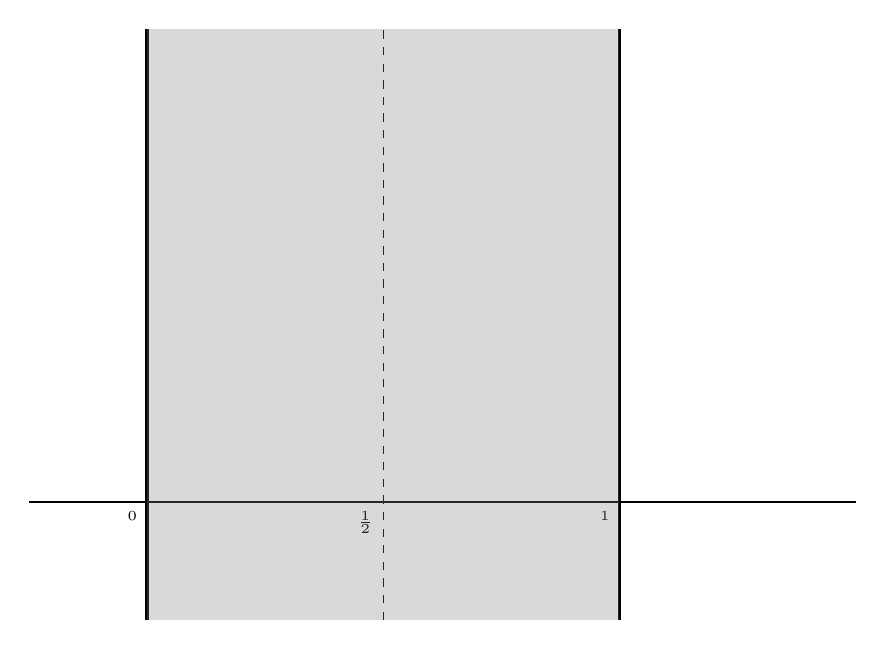
\begin{tikzpicture}[scale=3]
          \def\xmin{-0.5} \def\xmax{3}
          \def\ymin{-0.5} \def\ymax{2}
          \draw[thick] (\xmin,0) -- (\xmax,0);
          \draw[very thick] (0,\ymin) -- (0,\ymax);
          \draw[very thick] (2,\ymin) -- (2,\ymax);
          \draw[dashed] (1,\ymin) -- (1,\ymax);

          \node at (0,0) [below left] {\tiny{$0$}};
          \node at (1,0) [below left] {\tiny{$\frac{1}{2}$}};
          \node at (2,0) [below left] {\tiny{$1$}};

          \begin{scope}
              \path[clip] (0,\ymin) -- (0,\ymax) -- (2,\ymax) -- (2,\ymin) -- cycle;
              \fill[gray,opacity=0.3] (0,\ymin) rectangle (2,\ymax);
          \end{scope}
        \end{tikzpicture}
        \caption{The critical strip and line of Selberg class $L$-functions}
        \label{fig:critical_strip}
      \end{figure}
  \section{The Riemann Zeta Function}\label{sec:The_Riemann_Zeta_Function}
    \subsection*{The Definition \& Euler Product of \texorpdfstring{$\z$}{z}(s)}
      The \textbf{Riemann zeta function}\index{Riemann zeta function} or simply the \textbf{zeta function}\index{zeta function} $\z(s)$ is defined to be the Dirichlet series
      \[
        \z(s) = \sum_{n \ge 1}\frac{1}{n^{s}}.
      \]
      This is the prototypical example of a Dirichlet series as all the coefficients are $1$. Our main goal is to show that $\z(s)$ belongs to the Selberg class. As the coefficients are trivially polynomially bounded, $\z(s)$ is absolutely uniformly convergent on compacta for $\Re(s) > 1$. Also note that $\z(s)$ is necessiarly nonzero in this region. Determining the Euler product is also an easy matter. As the coefficients are obviously completely multiplicative, we have the degree $1$ Euler product
      \[
        \z(s) = \prod_{p}(1-p^{-s})^{-1},
      \]
      in this region as well. The local factor at $p$ is $(1-p^{-s})^{-1}$ with local root $1$. In particular, we have shown that the zeta function satisfies property (i) of the Selberg class and we package this into a theorem:

      \begin{theorem}
        For $\Re(s) > 1$,
        \[
          \z(s) = \sum_{n \ge 1}\frac{1}{n^{s}} = \prod_{p}(1-p^{-s})^{-1},
        \]
        is absolutely uniformly convergent on compacta with degree $1$ Euler product.
      \end{theorem}
    \subsection*{The Integral Representation of \texorpdfstring{$\z$}{z}(s): Part I}
      Riemann's ingenious insight was to analytically continue $\z(s)$. By this, he meant to find a representation of $\z(s)$ that is defined on a larger region that $\Re(s) > 1$. This is the approach we will take, and the argument follows the same line of reasoning as that of Riemann. We consider the gamma function $\G\left(\frac{s}{2}\right)$:
      \[
        \G\left(\frac{s}{2}\right) = \int_{0}^{\infty}e^{-x}x^{\frac{s}{2}}\,\frac{dx}{x}.
      \]

      \begin{remark}
        We have chosen to express the gamma function in terms of the measure $\frac{dx}{x}$ instead of $dx$. This is a tactical change for two reasons. The first is that $\frac{dx}{x}$ is invariant under the change of variables $x \to Cx$ for any constant $C$. The second is that under the change of variables $x \to \frac{1}{x}$ we have $\frac{dx}{x} \to -\frac{dx}{x}$ but the bounds of integration are also flipped. So we may leave the measure invariant provided we dont flip the bounds of integration. These types of change of variables are essential in the study of $L$-functions which motivates the use of this measure.
      \end{remark}

      Performing the change of variables $x \to \pi n^{2}x$ for fixed $n \ge 1$ yields
      \begin{equation}\label{equ:gamma_integral_substitution}
        \G\left(\frac{s}{2}\right) = \pi^{\frac{s}{2}} n^{s}\int_{0}^{\infty}e^{-\pi n^{2}x}x^{\frac{s}{2}}\,\frac{dx}{x}.
      \end{equation}
      Dividing by $\pi^{\frac{s}{2}}n^{s}$ and summing over $n \ge 1$, we see that for $\Re(s) > 1$,
      \begin{align*}
        \pi^{-\frac{s}{2}}\G\left(\frac{s}{2}\right)\z(s) &= \sum_{n \ge 1}\int_{0}^{\infty}e^{-\pi n^{2}x}x^{\frac{s}{2}}\,\frac{dx}{x} \\
        &= \int_{0}^{\infty}\sum_{n \ge 1}e^{-\pi n^{2}x}x^{\frac{s}{2}}\,\frac{dx}{x} && \text{DCT} \\
        &= \int_{0}^{\infty}\w(x)x^{\frac{s}{2}}\,\frac{dx}{x},
      \end{align*}
      where we set
      \[
        \w(x) = \sum_{n \ge 1}e^{-\pi n^{2}x}.
      \]
      Therefore we have an integral representation
      \begin{equation}\label{equ:integral_representation_zeta_1}
        \z(s) = \frac{\pi^{\frac{s}{2}}}{\G\left(\frac{s}{2}\right)}\int_{0}^{\infty}\w(x)x^{\frac{s}{2}}\,\frac{dx}{x}.
      \end{equation}
      This was essentially Riemann's insight: rewrite the zeta function in terms of the Gamma function. Unfortunately, we cannot proceed until we understand $\w(x)$. So we will make a slight detour and come back to the integral representation after.
    \subsection*{Jacobi's Theta Function \texorpdfstring{$\vt(s)$}{v(s)}}
      \textbf{Jacobi's theta function}\index{Jacobi's theta function} $\vt(s)$ is defined for $\Re(s) > 0$ by
      \[
        \vt(s) = \sum_{n \in \Z}e^{-\pi n^{2}s} = 1+2\sum_{n \ge 1}e^{-\pi n^{2}a}.
      \]
      It is absolutely uniformly convergent on compacta in this region by the ratio test. It's relation to $\w(s)$ is the identity
      \begin{equation}\label{equ:omega_theta_relationship_for_zeta}
        \w(s) = \frac{\vt(s)-1}{2}.
      \end{equation}
      The essential fact about Jacobi's theta function we will need is the following transformation law due to Jacobi and that was known to Riemann:

      \begin{theorem}
        For $\Re(s) > 0$,
        \[
          \vt(s) = \frac{1}{\sqrt{s}}\vt\left(\frac{1}{s}\right),
        \]
        where we take the principal branch of the square root.
      \end{theorem}
      \begin{proof}
        By the identity theorem it suffices to prove this on a set containg a limit point. We will prove this on the right-half of the real line, so take $s$ real with $s > 0$. Set $f(x) = e^{-\pi x^{2}s}$. Then $f(x)$ is a Schwarz function. We compute its Fourier transform:
        \[
          \hat{f}(t) = \int_{-\infty}^{\infty}f(x)e^{-2\pi itx}\,dx = \int_{-\infty}^{\infty}e^{-\pi x^{2}s}e^{-2\pi itx}\,dx = \int_{-\infty}^{\infty}e^{-\pi(x^{2}s+2itx)}\,dx.
        \]
        Making the change of variables $x \to \frac{x}{\sqrt{s}}$, the last integral above becomes
        \[
          \frac{1}{\sqrt{s}}\int_{-\infty}^{\infty}e^{-\pi\left(x^{2}+\frac{2itx}{\sqrt{s}}\right)}.
        \]
        Complete the square in the exponent by noticing
        \[
          -\pi\left(x^{2}+\frac{2itx}{\sqrt{s}}\right) = -\pi\left(\left(x+\frac{it}{\sqrt{s}}\right)^{2}+\frac{t^{2}}{s^{2}}\right),
        \]
        where we take the principal branch of the square root. Taking exponentials, this implies that the previous integral is equal to
        \[
          \frac{e^{-\frac{\pi t^{2}}{s}}}{\sqrt{s}}\int_{-\infty}^{\infty}e^{-\pi\left(x+\frac{it}{\sqrt{s}}\right)^{2}}\,dx.
        \]
        We now treat this last integral as a complex integral. That is,
        \[
          \int_{-\infty}^{\infty}e^{-\pi\left(x+\frac{it}{\sqrt{s}}\right)^{2}}\,dx = \int_{\Im(z) = 0}e^{-\pi\left(z+\frac{it}{\sqrt{s}}\right)^{2}}\,dz = \int_{\Im(z) = \frac{t}{\sqrt{s}}}e^{-\pi z^{2}}\,dz,
        \]
        where in the last equality we have made the change of variables $z \to z-\frac{it}{\sqrt{s}}$. Now fix $T > 0$ and let $R_{T}$ be the positively oriented rectangle bounded by the lines $\Im(z) = 0$, $\Im(z) = \frac{t}{\sqrt{s}}$, $\Re(z) = -T$ and $\Re(z) = T$. Consider
        \[
          \lim_{T \to \infty}\int_{R_{T}}e^{-\pi z^{2}}\,dz.
        \]
        On the one hand, the residue theorem implies that the integral is the sum of a $2\pi i$ multiple of the residues in the rectangle $R_{T}$ and so the limit is the sum of a $2\pi i$ multiple of the residues in the strip bounded by $\Im(z) = 0$ and $\Im(z) = \frac{t}{\sqrt{s}}$. Since $e^{-\pi\left(z+\frac{it}{\sqrt{s}}\right)^{2}}$ is entire, this is zero. On the other hand, we can decompose the integral as
        \[
          \int_{\Im(z) = 0}e^{-\pi z^{2}}\,dz+\lim_{T \to \infty}\int_{0}^{\frac{t}{\sqrt{s}}}e^{-\pi(iz+T)^{2}}\,dz-\int_{\Im(z) = \frac{t}{\sqrt{s}}}e^{-\pi z^{2}}\,dz-\lim_{T \to \infty}\int_{0}^{\frac{t}{\sqrt{s}}}e^{-\pi(iz-T)^{2}}\,dz.
        \]
        Since $(iz \pm T)^{2} \ll_{z} T^{2}$, the integrands of the second and fourth terms decay to zero as $T \to \infty$. Hence the corresponding limits of integrals is zero. Putting these two computations together shows
        \[
          \int_{\Im(z) = \frac{t}{\sqrt{s}}}e^{-\pi z^{2}}\,dz = \int_{\Im(z) = 0}e^{-\pi z^{2}}\,dz = \int_{-\infty}^{\infty}e^{-\pi x^{2}}\,dx.
        \]
        So back to the integral at hand, the above chain of equalities implies
        \[
          \frac{e^{-\frac{\pi t^{2}}{s}}}{\sqrt{s}}\int_{-\infty}^{\infty}e^{-\pi\left(x+\frac{it}{\sqrt{s}}\right)^{2}}\,dx = \frac{e^{-\frac{\pi t^{2}}{s}}}{\sqrt{s}}\int_{-\infty}^{\infty}e^{-\pi x^{2}}\,dx = \frac{e^{-\frac{\pi t^{2}}{s}}}{\sqrt{s}},
        \]
        where the last equality follows because the last integral above is $1$ since it is the Gaussian integral (see \cref{append:Special_Integrals}). The Poisson summation formula then gives the middle equality in the following chain:
        \[
          \vt(s) = \sum_{n \in \Z}f(n) = \sum_{t \in \Z}\hat{f}(t) = \frac{1}{\sqrt{s}}\vt\left(\frac{1}{s}\right).
        \]
      \end{proof}

      Take note that the key ingredient in the proof was the Poisson summation formula. This is typical of a larger relaity when one needs to prove transformation laws. Also, the method of changing the line of integration from $\Im(z) = \frac{t}{\sqrt{s}}$ to $\Im(z) = 0$ works in a much more general setting and is a very useful analytic technique called \textbf{shifting the line of integration}\index{shifting the line of integration}:

      \begin{method}[Shifting the line of integration]
        Suppose we are given an integral
        \[
          \int_{\Re(z) = a}f(z)\,dz \quad \text{or} \quad \int_{\Im(z) = a}f(z)\,dz,
        \]
        and some real $b \neq a$ such that the following hold:
        \begin{enumerate}[label=(\roman*)]
          \item $f$ is meromorphic on a strip containing $a$ and $b$ in its interior.
          \item $f$ is holomorphic about $\Re(z) = a,b$ or $\Im(z) = a,b$ respectively.
          \item $f(z) \to 0$ as $\Im(z) \to \infty$ or $f(z) \to 0$ as $\Re(z) \to \infty$ respectively.
        \end{enumerate}
        To collect these cases, let $(a)$ stand for the line $\Re(z) = a$ or $\Im(z) = a$ with positive orientation respectively. Then the line of integration $(a)$ can be shifted to the line of integration $(b)$ with the possible addition of residues. Take a rectangle $R_{T}$ given positive orientation and with its edges on $(a)$ and $(b)$ respectively and consider
        \[
          \lim_{T \to \infty}\int_{R_{T}}f(z)\,dz.
        \]
        On the one hand, the residue Theorem implies the integral is a sum of a $2\pi i$ multiple of the residues $r_{i}$ in the rectangle $R_{T}$ and hence the limit is a sum of a $2\pi i$ multiple of the residues in the strip bounded by $(a)$ and $(b)$. On the other hand, the integral can be decomposed into a sum of four integrals along the edges of $R_{T}$ and by taking the limit the edges other than $(a)$ and $(b)$ will tend to zero because of the assumptions on $f$. The remaining two pieces is the difference between the integral along $(a)$ and $(b)$. So in total,
        \[
          \int_{(a)}f(z)\,dz = \int_{(b)}f(z)\,dz+2\pi i\sum_{r_{i} \in I}\Res_{z = r_{i}}f(z).
        \]
      \end{method}

      A particular application of interest is when the integral in question is real and over the entire real line, the integrand is entire as a complex function, and one is trying to shift the line of integration of the complexified integral to $\Im(z) = a$. In this case, shifting the line of integration amounts to making the change of variables $x \to x-ia$ without affecting the initial region of integration in the real integral. For example, in the proof of the transformation law for Jacobi's theta function this amounts to saying that the change of variables $x \to \frac{x}{\sqrt{s}}-\frac{it}{\sqrt{s}}$ is permitted without affecting the line of integration. We will appeal to this application often when proving transformation laws and one should become familiar with it. This completes our interest in Jacobi's theta function.
    \subsection*{The Integral Representation of \texorpdfstring{$\z$}{z}(s): Part II}
      Returning to the zeta function, we split the integral in \cref{equ:integral_representation_zeta_1} into two pieces
      \begin{equation}\label{equ:symmetric_integral_zeta_split}
        \int_{0}^{\infty}\w(x)x^{\frac{s}{2}}\,\frac{dx}{x} = \int_{0}^{1}\w(x)x^{\frac{s}{2}}\,\frac{dx}{x}+\int_{1}^{\infty}\w(x)x^{\frac{s}{2}}\,\frac{dx}{x}.
      \end{equation}
      Since $\w(x)$ has exponential decay to zero as $x \to \infty$, the second piece is absolutely uniformly bounded on compacta for $\Re(s) > 1$ by \cref{met:decay_compacta_integral}. Hence it defines an analytic function there. The idea now is to rewrite the first piece in the same form and symmetrize the result as much as possible. We being by performing a change of variables $x \to \frac{1}{x}$ to the first piece to obtain
      \[
        \int_{1}^{\infty}\w\left(\frac{1}{x}\right)x^{-\frac{s}{2}}\,\frac{dx}{x}
      \]
      Now the transformation law for $\vt(x)$ and \cref{equ:omega_theta_relationship_for_zeta} together imply
      \[
        \w\left(\frac{1}{x}\right) = \frac{\vt\left(\frac{1}{x}\right)-1}{2} = \frac{\sqrt{x}\vt(x)-1}{2} = \frac{\sqrt{x}(2\w(x)+1)-1}{2} = \sqrt{x}\w(x)+\frac{\sqrt{x}}{2}-\frac{1}{2}.
      \]
      Therefore
      \begin{align*}
        \int_{1}^{\infty}\w\left(\frac{1}{x}\right)x^{-\frac{s}{2}}\,\frac{dx}{x} &= \int_{1}^{\infty}\left(\sqrt{x}\w(x)+\frac{\sqrt{x}}{2}-\frac{1}{2}\right)x^{-\frac{s}{2}}\,\frac{dx}{x} \\
        &= \int_{1}^{\infty}\w(x)x^{\frac{1-s}{2}}\,\frac{dx}{x}+\int_{1}^{\infty}\frac{x^{\frac{1-s}{2}}}{2}\,\frac{dx}{x}-\int_{1}^{\infty}\frac{x^{-\frac{s}{2}}}{2}\,\frac{dx}{x} \\
        &= \int_{1}^{\infty}\w(x)x^{\frac{1-s}{2}}\,\frac{dx}{x}+\frac{1}{1-s}-\frac{1}{s} \\
        &= \int_{1}^{\infty}\w(x)x^{\frac{1-s}{2}}\,\frac{dx}{x}-\frac{1}{s(1-s)}.
      \end{align*}
      Substituting this back into \cref{equ:symmetric_integral_zeta_split} with \cref{equ:integral_representation_zeta_1} yields the following result:

      \begin{theorem}
        For $\Re(s) > 1$,
        \[
          \z(s) = \frac{\pi^{\frac{s}{2}}}{\G\left(\frac{s}{2}\right)}\left[-\frac{1}{s(1-s)}+\int_{1}^{\infty}\w(x)x^{\frac{1-s}{2}}\,\frac{dx}{x}+\int_{1}^{\infty}\w(x)x^{\frac{s}{2}}\,\frac{dx}{x}\right].
        \]
      \end{theorem}

      This integral representation will give analytic continuation. To see this, first observe that we know everything outside the backets is entire. Everything inside the brackets except for the first integral is analytic for $\Re(s) > 1$. Thus the first integral must be analytic in this region too. Since the two integrals are interchanged as $s \to 1-s$ and the rational term $-\frac{1}{s(1-s)}$ is invariant, the right-hand side is analytic for $\Re(s) < 0$. This gives the analytic continuation of $\z(s)$ to the region
      \[
        \left\{s \in \C:\left|\Re(s)-\frac{1}{2}\right| > \frac{1}{2}\right\}.
      \]
    \subsection*{The Functional Equation, Critical Strip \& Residue of \texorpdfstring{$\z$}{z}(s)}
      An immediate consequence of the symmetry of the integral representation is the functional equation:
      \[
        \frac{\G\left(\frac{s}{2}\right)}{\pi^{\frac{s}{2}}}\z(s) = \frac{\G\left(\frac{1-s}{2}\right)}{\pi^{\frac{1-s}{2}}}\z(1-s).
      \]
      We identify the gamma factor as
      \[
        \g(s,\z) = \pi^{-\frac{s}{2}}\G\left(\frac{s}{2}\right),
      \]
      with $\k = \frac{s}{2}$ the only local parameter at infinity. Clearly it satisfies the required bounds. The conductor is $q(\z) = 1$ so no primes ramify. The completed zeta function is
      \[
        \L(s,\z) = \pi^{-\frac{s}{2}}\G\left(\frac{s}{2}\right)\z(s),
      \]
      with functional equation
      \[
        \L(s,\z) = \L(1-s,\z).
      \]
      This is the functional equation of $\z(s)$ and in this case is just a reformulation of the previous functional equation. From it we find that the root number is $\e(\z) = 1$ and that $\z$ is self-dual. All together, we have shown that $\z$ satisfies properties (ii)-(iv) of the Selberg class.

      Having obtained the funtional equation, we now use the integral representation to obtain meromorphic continuation of $\z(s)$ inside the critical strip. From the integral representation and functional equation, we have
      \begin{equation}\label{equ:integral_representation_zeta_2}
        \z(s) = \frac{1}{\g(s,\z)}\left[-\frac{1}{s(1-s)}+\int_{1}^{\infty}\w(x)x^{\frac{1-s}{2}}\,\frac{dx}{x}+\int_{1}^{\infty}\w(x)x^{\frac{s}{2}}\,\frac{dx}{x}\right].
      \end{equation}
      To get continuation inside of the critical strip, we show that the two integrals are absolutely uniformly bounded on compacta for $|\Re(s)-\frac{1}{2}| \le \frac{1}{2}$. This follows by \cref{met:decay_compacta_integral} (we could have gotten this continuation earlier but we didn't need it until now). If we assume $s \neq 0,1$, then the analytic continuation to the inside of the critical strip follows since the fractional term $\frac{1}{s(1-s)}$ is holomorphic there. The cases $s = 0,1$ require separate inspection. When $s = 0$, $\g(s,\z)$ has a simple pole coming from the gamma factor, and therefore its reciprocal has a simple zero. This cancels the corresponding simple pole of $\frac{1}{s(1-s)}$ and therefore $\z(s)$ has a removable singularity and thus is holomorphic at $s = 0$. At $s = 1$, $\g(s,\z)$ is nonzero, and so $\g(s)$ has a simple pole. Therefore $\g(s)$ has meromorphic continuation to all of $\C$ with a simple pole at $s = 1$.

      We can now show that the order of $\z(s)$ is $1$ and conclude that it satisfies property (v) of the Selberg class, and is therefore an $L$-function belonging to the Selberg class. As there is only a simple pole at $s = 1$, multiply by $(s-1)$ to clear the polar divisor. Now the integral in the integral representation is absolutely bounded, so computing the order amounts to estimating the gamma factor. Since the reciprocal of the gamma function is order $1$ and $\Re(s)$ is bounded, we have
      \begin{equation}\label{equ:zeta_function_gamma_factor_order_1}
        \frac{1}{\g(s,\z)} \ll_{\e} e^{|s|^{1+\e}},
      \end{equation}
      for any $\e > 0$. So the reciprocal of the gamma factor is of the same order. Then \cref{equ:zeta_function_gamma_factor_order_1,equ:integral_representation_zeta_2} together imply
      \[
        (s-1)\z(s) \ll_{\e} e^{|s|^{1+\e}}.
      \]
      So $(s-1)\z(s)$ is of order $1$, and then $\z(s)$ is as well after removing the polar factor. Having shown the analytic continuation of $\z(s)$, and verified that it belongs to the Selberg class, there is only one thing left to do. This is to compute the residue of $\z(s)$ at $s = 1$:

      \begin{proposition}\label{prop:zeta_residue}
        \[
          \Res_{s = 1}\z(s) = 1.
        \]
      \end{proposition}
      \begin{proof}
        The only term in the integral representation of $\z(s)$ contributing to the pole is $-\frac{1}{\g(s,\z)}\frac{1}{s(1-s)}$. Observe
        \[
          \lim_{s \to 1}\frac{1}{\g(s,\z)} = \lim_{s \to 1}\frac{\pi^{\frac{s}{2}}}{\G\left(\frac{s}{2}\right)} = 1,
        \]
        because $\G\left(\frac{1}{2}\right) = \sqrt{\pi}$. Therefore
        \[
          \Res_{s = 1}\z(s) = \Res_{s = 1}-\frac{1}{\g(s,\z)}\frac{1}{s(1-s)} = \Res_{s = 1}-\frac{1}{s(1-s)} = \lim_{s \to 1}-\frac{(s-1)}{s(1-s)} = 1.
        \]
      \end{proof}

      We summarize all of our work into the following theorem:

      \begin{theorem}
        $\z(s)$ is a Selberg class $L$-function. It admits meromorphic continuation to $\C$ via the integral representation
        \[
          \z(s) = \frac{\pi^{\frac{s}{2}}}{\G\left(\frac{s}{2}\right)}\left[-\frac{1}{s(1-s)}+\int_{1}^{\infty}\w(x)x^{\frac{1-s}{2}}\,\frac{dx}{x}+\int_{1}^{\infty}\w(x)x^{\frac{s}{2}}\,\frac{dx}{x}\right],
        \]
        with a simple pole at $s = 1$ of residue $1$, and possesses the functional equation
        \[
          \pi^{-\frac{s}{2}}\G\left(\frac{s}{2}\right)\z(s) = \L(s,\z) = \L(1-s,\z).
        \]
      \end{theorem}

      Lastly, we note that by virtue of the functional equation we can also compute $\z(0)$ as well. Indeed, since $\Res_{s = 1}\z(s) = 1$, we have
        \[
          \lim_{s \to 1}(s-1)\L(s,\z) = \Res_{s = 1}\z(s)\lim_{s \to 1}\pi^{-\frac{s}{2}}\G\left(\frac{s}{2}\right) = 1.
        \]
        In other words, $\L(s,\z)$ has a simple pole at $s = 1$ with residue $1$ too. Since the completed zeta function is completely symmetric as $s \to 1-s$, it has a simple pole at $s = 0$ with residue $1$. Hence
        \[
          1 = \lim_{s \to 1}(s-1)\L(1-s,\z) = \Res_{s = 1}\G\left(\frac{1-s}{2}\right)\lim_{s \to 1}\pi^{-\frac{1-s}{2}}\z(1-s) = -2\z(0),
        \]
        because $\Res_{s = 0}\G(s) = 1$. Therefore $\z(0) = -\frac{1}{2}$.
  \section{Dirichlet \texorpdfstring{$L$}{L}-functions}
    \subsection*{The Definition \& Euler Product of \texorpdfstring{$L(s,\chi)$}{L(s,x)}}
      To every Dirichlet character $\chi$ there is an associated $L$-function. Throughout we will let $m$ denote the modulus and $q$ the conductor of $\chi$ respectively. The \textbf{Dirichlet $L$-function}\index{Dirichlet $L$-function} $L(s,\chi)$ attached to the Dirichlet character $\chi$ is defined by the Dirichlet series
      \[
        L(s,\chi) = \sum_{n \ge 1}\frac{\chi(n)}{n^{s}}.
      \]
      Since $\chi(n) = 0$ if $(n,m) > 1$, the above sum can be restricted to all integers relatively prime to $m$. We first obtain convergence in a half-plane. As $|\chi(n)| \ll 1$, $L(s,\chi)$ is absolutely uniformly convergent on compacta for $\Re(s) > 1$ just as is the case for $\z(s)$. Because $\chi$ is completely multiplicative we also have the degree $1$ Euler product,
      \[
        L(s,\chi) = \prod_{p}(1-\chi(p)p^{-s})^{-1} = \prod_{p \nmid m}(1-\chi(p)p^{-s})^{-1},
      \]
      in this region as well. The last equality holds because if $p \mid m$ we have $\chi(p) = 0$. So for $p \mid m$, the local factor at $p$ is $1$ with local root $0$. For $p \nmid m$ the local factor at $p$ is $(1-\chi(p)p^{-s})^{-1}$ with local root $\chi(p)$. Now if $\chi$ is induced by $\wtilde{\chi}$, then $\chi(p) = \wtilde{\chi}(p)$ if $p \nmid q$ and $\chi(p) = 0$ if $p \mid m$ so that
      \[
        L(s,\chi) = \prod_{p \nmid m}(1-\wtilde{\chi}(p)p^{-s})^{-1} = \prod_{p}(1-\wtilde{\chi}(p)p^{-s})^{-1}\prod_{p \mid m}(1-\wtilde{\chi}(p)p^{-s}) = L(s,\wtilde{\chi})\prod_{p \mid m}(1-\wtilde{\chi}(p)p^{-s}).
      \]
      Therefore $L(s,\chi)$ belongs to the Selberg class if and only if $L(s,\wtilde{\chi})$ does. So we may assume $\chi$ is primitive. We may assume further that $q > 1$ because if not $\chi$ is principal which means $\wtilde{\chi}$ is trivial so that $L(s,\wtilde{\chi}) = \z(s)$, and this $L$-function already belongs to the Selberg class. Our main goal is now to show that $L(s,\chi)$ is a Selberg class $L$-function when $\chi$ is primitive and $q > 1$. We have already shown that $L(s,\chi)$ satisfies property (i) of the Selberg class and we package this into a theorem:

      \begin{theorem}
        Let $\chi$ be a primitive Dirichlet character with conductor $q > 1$. For $\Re(s) > 1$,
        \[
          L(s,\chi) = \sum_{n \ge 1}\frac{\chi(n)}{n^{s}} = \prod_{p \nmid q}(1-\chi(p)p^{-s})^{-1},
        \]
        is absolutely uniformly convergent on compacta with degree $1$ Euler product.
      \end{theorem}
    \subsection*{The Integral Representation of \texorpdfstring{$L(s,\chi)$}{L(s,x)}: Part I}
      To find the integral representation for $L(s,\chi)$ we proceed similarly to $\z(s)$. However, the following will depend if $\chi$ is even or odd, so to handle both cases simultaneously set $\d_{\chi}$ so that $\chi(-1) = (-1)^{\d_{\chi}}$. That is, $\d_{\chi} = 0,1$ according to whether $\chi$ is even or odd. Note that $\d_{\cchi} = \d_{\chi}$. Making the substitution $s \to s+\d_{\chi}$ in \cref{equ:gamma_integral_substitution} and multiplying by $\chi(n)$ yields
      \[
        \chi(n)\G\left(\frac{s+\d_{\chi}}{2}\right) = \pi^{\frac{s+\d_{\chi}}{2}} n^{s}\int_{0}^{\infty}\chi(n)n^{\d_{\chi}}e^{-\pi n^{2}x}x^{\frac{s+\d_{\chi}}{2}}\,\frac{dx}{x},
      \]
      after moving the $n^{\d_{\chi}}$ on the inside of the integral. Dividing by $\pi^{\frac{s+\d_{\chi}}{2}}n^{s}$ and summing over $n \ge 1$, we see that for $\Re(s) > 1$,
      \begin{align*}
        \pi^{-\frac{s+\d_{\chi}}{2}}\G\left(\frac{s+\d_{\chi}}{2}\right)L(s,\chi) &= \sum_{n \ge 1}\int_{0}^{\infty}\chi(n)n^{\d_{\chi}}e^{-\pi n^{2}x}x^{\frac{s+\d_{\chi}}{2}}\,\frac{dx}{x} \\
        &= \int_{0}^{\infty}\sum_{n \ge 1}\chi(n)n^{\d_{\chi}}e^{-\pi n^{2}x}x^{\frac{s+\d_{\chi}}{2}}\,\frac{dx}{x} && \text{DCT} \\
        &= \int_{0}^{\infty}\w_{\chi}(x)x^{\frac{s+\d_{\chi}}{2}}\,\frac{dx}{x},
      \end{align*}
      where we set
      \[
        \w_{\chi}(x) = \sum_{n \ge 1}\chi(n)n^{\d_{\chi}}e^{-\pi n^{2}x}.
      \]
      Therefore we have an integral representation
      \begin{equation}\label{equ:integral_representation_Dirichlet_L-functions_1}
        L(s,\chi) = \frac{\pi^{\frac{s+\d_{\chi}}{2}}}{\G\left(\frac{s+\d_{\chi}}{2}\right)}\int_{0}^{\infty}\w_{\chi}(x)x^{\frac{s+\d_{\chi}}{2}}\,\frac{dx}{x},
      \end{equation}
      and just like $\z(s)$ we need to find a transformation law for $\w_{\chi}(x)$ before we can proceed.
    \subsection*{The Dirichlet Theta Function \texorpdfstring{$\vt_{\chi}(s)$}{v_x(s)}}
      The \textbf{Dirichlet theta function}\index{Dirichlet theta function} $\vt_{\chi}(s)$, attached to the character $\chi$, is defined for $\Re(s) > 0$ by
      \[
        \vt_{\chi}(s) = \sum_{n \in \Z}\chi(n)n^{\d_{\chi}}e^{-\pi n^{2}s} = 2\sum_{n \ge 1}\chi(n)n^{\d_{\chi}}e^{-\pi n^{2}s}.
      \]
      It is absolutely uniformly convergent on compacta in this region by the ratio test. Notice that the term corresponding to $n = 0$ vanishes because $\chi(0) = 0$, and $\chi(n)n^{\d_{\chi}} = \chi(-n)(-n)^{\d_{\chi}}$ so that the $n$-th and $(-n)$-th terms agree. Therefore the relationship between the twisted theta function and $\w_{\chi}(s)$ is
      \begin{equation}\label{equ:twisted_omega_theta_relationship_for_Dirichlet_L-functions}
        \w_{\chi}(s) = \frac{\vt_{\chi}(s)}{2}.
      \end{equation}

      \begin{remark}
        \cref{equ:twisted_omega_theta_relationship_for_Dirichlet_L-functions} is a slightly less complex relationship that \cref{equ:omega_theta_relationship_for_zeta}. This is because assuming $q > 1$ means $\chi(0) = 0$.
      \end{remark}

      The essential fact about the twisted theta function we will need is the following transformation law similar to Jacobi's theta function:

      \begin{theorem}
        Let $\chi$ be a primitive Dirichlet character with conductor $q > 1$. For $\Re(s) > 0$,
        \[
          \vt_{\chi}(s) = \frac{\e_{\chi}}{i^{\d_{\chi}}q^{\frac{1}{2}+\d_{\chi}}s^{\frac{1}{2}+\d_{\chi}}}\vt_{\cchi}\left(\frac{1}{q^{2}s}\right).
        \]
        where we take the principal branch of the square root.
      \end{theorem}
      \begin{proof}
        By the identity theorem it suffices to prove this on a set containg a limit point. We will prove this on the right-half of the real line, so take $s$ real with $s > 0$. Since $\chi$ is $q$-periodic, we can write
        \[
          \vt_{\chi}(s) = \sum_{a \tmod{q}}\chi(a)\sum_{m \in \Z}(mq+a)^{\d_{\chi}}e^{-\pi(mq+a)^{2}s}.
        \]
        Set $f(x) = (xq+a)^{\d_{\chi}}e^{-\pi(xq+a)^{2}s}$. Then $f(x)$ is a Schwarz function. We compute its Fourier transform:
        \[
          \hat{f}(t) = \int_{-\infty}^{\infty}f(x)e^{-2\pi itx}\,dx = \int_{-\infty}^{\infty}(xq+a)^{\d_{\chi}}e^{-\pi(xq+a)^{2}s}e^{-2\pi itx}\,dx = \int_{-\infty}^{\infty}(xq+a)^{\d_{\chi}}e^{-\pi((xq+a)^{2}s+2itx)}\,dx.
        \]
        By performing the change of variables $x \to \frac{x}{q\sqrt{s}}-\frac{a}{q}$, the last integral above becomes
        \[
          \frac{e^{\frac{2\pi iat}{q}}}{qs^{\frac{1+\d_{\chi}}{2}}}\int_{-\infty}^{\infty}x^{\d_{\chi}}e^{-\pi\left(x^{2}+\frac{2itx}{q\sqrt{s}}\right)}\,dx.
        \]
        Complete the square in the exponent by observing
        \[
          -\pi\left(x^{2}+\frac{2itx}{q\sqrt{s}}\right) = -\pi\left(\left(x+\frac{it}{q\sqrt{s}}\right)^{2}+\frac{t^{2}}{q^{2}s}\right),
        \]
        where we take the principal branch of the square root. Taking exponentials, this implies that the previous integral is equal to
        \[
          \frac{e^{\frac{2\pi iat}{q}}e^{-\frac{\pi t^{2}}{q^{2}s}}}{qs^{\frac{1+\d_{\chi}}{2}}}\int_{-\infty}^{\infty}x^{\d_{\chi}}e^{-\pi\left(x+\frac{it}{q\sqrt{s}}\right)^{2}}\,dx.
        \]
        The change of variables $x \to x-\frac{it}{q\sqrt{s}}$ is permitted without affecting the line of integration by viewing the integral as a complex integral, noting that the integrand is entire as a complex function, and shifting the line of integration. This gives
        \[
          \frac{e^{\frac{2\pi iat}{q}}e^{-\frac{\pi t^{2}}{q^{2}s}}}{qs^{\frac{1+\d_{\chi}}{2}}}\int_{-\infty}^{\infty}\left(x-\frac{it}{q\sqrt{s}}\right)^{\d_{\chi}}e^{-\pi x^{2}}\,dx = \frac{e^{\frac{2\pi iat}{q}}e^{-\frac{\pi t^{2}}{q^{2}s}}}{qs^{\frac{1+\d_{\chi}}{2}}}\int_{-\infty}^{\infty}\left(x+\frac{t}{iq\sqrt{s}}\right)^{\d_{\chi}}e^{-\pi x^{2}}\,dx.
        \]
        If $\d_{\chi} = 0$, we obtain
        \[
          \frac{e^{\frac{2\pi iat}{q}}e^{-\frac{\pi t^{2}}{q^{2}s}}}{qs^{\frac{1+\d_{\chi}}{2}}}\int_{-\infty}^{\infty}e^{-\pi x^{2}}\,dx = \frac{e^{\frac{2\pi iat}{q}}e^{-\frac{\pi t^{2}}{q^{2}s}}}{qs^{\frac{1+\d_{\chi}}{2}}},
        \]
        where the equality holds because the integral is $1$ since it is the Gaussian integral (see \cref{append:Special_Integrals}). If $\d_{\chi} = 1$, then by direct computation
        \[
          \int_{-\infty}^{\infty}xe^{-\pi x^{2}}\,dx = -\frac{1}{2\pi}e^{-\pi x^{2}}\bigg|_{-\infty}^{\infty} = 0,
        \]
        and thus the expression reduces to
        \[
          \frac{e^{\frac{2\pi iat}{q}}e^{-\frac{\pi t^{2}}{q^{2}s}}}{qs^{\frac{1+\d_{\chi}}{2}}}\int_{-\infty}^{\infty}\left(\frac{t}{iq\sqrt{s}}\right)e^{-\pi x^{2}}\,dx = \frac{e^{\frac{2\pi iat}{q}}e^{-\frac{\pi t^{2}}{q^{2}s}}}{qs^{\frac{1+\d_{\chi}}{2}}}\left(\frac{t}{iq\sqrt{s}}\right)\int_{-\infty}^{\infty}e^{-\pi x^{2}}\,dx = \frac{e^{\frac{2\pi iat}{q}}e^{-\frac{\pi t^{2}}{q^{2}s}}}{qs^{\frac{1+\d_{\chi}}{2}}}\left(\frac{t}{iq\sqrt{s}}\right),
        \]
        where the last equality follows because the last integral is the Gaussian integral again. Since $\left(\frac{t}{iq\sqrt{s}}\right)^{\d_{\chi}} = 1$ if $\d_{\chi} = 0$, we can compactly express both cases in the form
        \[
          \frac{e^{\frac{2\pi iat}{q}}e^{-\frac{\pi t^{2}}{q^{2}s}}}{qs^{\frac{1+\d_{\chi}}{2}}}\left(\frac{t}{iq\sqrt{s}}\right)^{\d_{\chi}}.
        \]
        The Poisson summation formula then gives the second equality in the following chain:
        \begin{align*}
          \vt_{\chi}(s) &= \sum_{a \tmod{q}}\chi(a)\sum_{m \in \Z}f(m) \\
          &= \sum_{a \tmod{q}}\chi(a)\sum_{t \in \Z}\hat{f}(t) \\
          &= \sum_{a \tmod{q}}\chi(a)\sum_{t \in \Z}\frac{e^{\frac{2\pi iat}{q}}e^{-\frac{\pi t^{2}}{q^{2}s}}}{qs^{\frac{1+\d_{\chi}}{2}}}\left(\frac{t}{iq\sqrt{s}}\right)^{\d_{\chi}} \\
          &= \frac{1}{i^{\d_{\chi}}q^{1+\d_{\chi}}s^{\frac{1}{2}+\d_{\chi}}}\sum_{a \tmod{q}}\chi(a)\sum_{t \in \Z}t^{\d_{\chi}}e^{\frac{2\pi i at}{q}}e^{-\frac{\pi t^{2}}{q^{2}s}} \\
          &= \frac{1}{i^{\d_{\chi}}q^{1+\d_{\chi}}s^{\frac{1}{2}+\d_{\chi}}}\sum_{t \in \Z}t^{\d_{\chi}}e^{-\frac{\pi t^{2}}{q^{2}s}}\sum_{a \tmod{q}}\chi(a)e^{\frac{2\pi i at}{q}} \\
          &= \frac{1}{i^{\d_{\chi}}q^{1+\d_{\chi}}s^{\frac{1}{2}+\d_{\chi}}}\sum_{t \in \Z}t^{\d_{\chi}}e^{-\frac{\pi t^{2}}{q^{2}s}}\tau(t,\chi) && \text{definition of $\tau(t,\chi)$}.
        \end{align*}
        Since $\chi$ is primitive, $\tau(t,\chi) = 0$ if $(t,q) > 1$ and otherwise $\tau(t,\chi) = \cchi(t)\tau(1,\chi)$ (see \cref{prop:Gauss_sum_reduction}). Therefore we have
        \[
          \frac{1}{i^{\d_{\chi}}q^{1+\d_{\chi}}s^{\frac{1}{2}+\d_{\chi}}}\sum_{t \in \Z}t^{\d_{\chi}}e^{-\frac{\pi t^{2}}{q^{2}s}}\tau(t,\chi) = \frac{\tau(1,\chi)}{i^{\d_{\chi}}q^{1+\d_{\chi}}s^{\frac{1}{2}+\d_{\chi}}}\sum_{t \in \Z}\cchi(t)t^{\d_{\chi}}e^{-\frac{\pi t^{2}}{q^{2}s}} = \frac{\tau(1,\chi)}{i^{\d_{\chi}}q^{1+\d_{\chi}}s^{\frac{1}{2}+\d_{\chi}}}\vt_{\cchi}\left(\frac{1}{q^{2}s}\right).
        \]
        Recalling that $\e_{\chi} = \frac{\tau(1,\chi)}{\sqrt{q}}$, all together we have
        \[
          \vt_{\chi}(s) = \frac{\e_{\chi}}{i^{\d_{\chi}}q^{\frac{1}{2}+\d_{\chi}}s^{\frac{1}{2}+\d_{\chi}}}\vt_{\cchi}\left(\frac{1}{q^{2}s}\right).
        \]
      \end{proof}
      The most striking property about this transformation law is that it relates $\vt_{\chi}(s)$ and $\vt_{\cchi}(s)$. Regardless, we can now exploit it to analytically continue $L(s,\chi)$.
    \subsection*{The Integral Representation of \texorpdfstring{$L(s,\chi)$}{L(s,x)}: Part II}
      Returning to $L(s,\chi)$, split the integral in \cref{equ:integral_representation_Dirichlet_L-functions_1} into two pieces
      \begin{equation}\label{equ:symmetric_integral_Dirichlet_L-functions_split}
        \int_{0}^{\infty}\w_{\chi}(x)x^{\frac{s+\d_{\chi}}{2}}\,\frac{dx}{x} = \int_{0}^{\frac{1}{q}}\w_{\chi}(x)x^{\frac{s+\d_{\chi}}{2}}\,\frac{dx}{x}+\int_{\frac{1}{q}}^{\infty}\w_{\chi}(x)x^{\frac{s+\d_{\chi}}{2}}\,\frac{dx}{x}.
      \end{equation}
      Since $\w_{\chi}(x)$ has exponential decay to zero as $x \to \infty$, the second piece is absolutely uniformly bounded on compacta for $\Re(s) > 1$ by \cref{met:decay_compacta_integral}. Hence it defines an analytic function there. We now rewrite the first piece in the same form and symmetrize the result as much as possible. Start by performing a change of variables $x \to \frac{1}{q^{2}x}$ to the first piece to obtain
      \[
        q^{-(s+\d_{\chi})}\int_{\frac{1}{q}}^{\infty}\w_{\chi}\left(\frac{1}{q^{2}x}\right)x^{-\frac{s+\d_{\chi}}{2}}\,\frac{dx}{x}.
      \]
      Now the transformation law for $\vt_{\chi}(x)$ and \cref{equ:twisted_omega_theta_relationship_for_Dirichlet_L-functions} together imply
      \begin{align*}
        \w_{\chi}\left(\frac{1}{q^{2}x}\right) &= \frac{\vt_{\chi}\left(\frac{1}{q^{2}x}\right)}{2} \\
        &= \frac{i^{\d_{\cchi}}q^{\frac{1}{2}+\d_{\cchi}}x^{\frac{1}{2}+\d_{\cchi}}}{\e_{\cchi}}\frac{\vt_{\cchi}(x)}{2} \\
        &= (-i)^{\d_{\cchi}}\e_{\chi}q^{\frac{1}{2}+\d_{\cchi}}x^{\frac{1}{2}+\d_{\cchi}}\frac{\vt_{\cchi}(x)}{2} && \text{\cref{prop:epsilon_factor_relationship} and $\chi(-1) = (-1)^{\d_{\chi}}$} \\
        &= \frac{\e_{\chi}q^{\frac{1}{2}+\d_{\cchi}}x^{\frac{1}{2}+\d_{\cchi}}}{i^{\d_{\cchi}}}\frac{\vt_{\cchi}(x)}{2} \\
        &= \frac{\e_{\chi}q^{\frac{1}{2}+\d_{\chi}}x^{\frac{1}{2}+\d_{\chi}}}{i^{\d_{\chi}}}\frac{\vt_{\cchi}(x)}{2} && \text{$\d_{\cchi} = \d_{\chi}$} \\
        &= \frac{\e_{\chi}q^{\frac{1}{2}+\d_{\chi}}x^{\frac{1}{2}+\d_{\chi}}}{i^{\d_{\chi}}}\w_{\cchi}(x).
      \end{align*}
      Therefore
      \begin{align*}
        q^{-(s+\d_{\chi})}\int_{\frac{1}{q}}^{\infty}\w_{\chi}\left(\frac{1}{q^{2}x}\right)x^{-\frac{s+\d_{\chi}}{2}}\,\frac{dx}{x} &= q^{-(s+\d_{\chi})}\int_{\frac{1}{q}}^{\infty}\left(\frac{\e_{\chi}q^{\frac{1}{2}+\d_{\chi}}x^{\frac{1}{2}+\d_{\chi}}}{i^{\d_{\chi}}}\w_{\cchi}(x)\right)x^{-\frac{s+\d_{\chi}}{2}}\,\frac{dx}{x} \\
        &= \frac{\e_{\chi}}{i^{\d_{\chi}}}q^{\frac{1}{2}-s}\int_{\frac{1}{q}}^{\infty}\w_{\cchi}(x)x^{\frac{(1-s)+\d_{\chi}}{2}}\,\frac{dx}{x}.
      \end{align*}
      Substituting this back into \cref{equ:symmetric_integral_Dirichlet_L-functions_split} with \cref{equ:integral_representation_Dirichlet_L-functions_1} yields
      \[
        L(s,\chi) = \frac{\pi^{\frac{s+\d_{\chi}}{2}}}{\G\left(\frac{s+\d_{\chi}}{2}\right)}\left[\frac{\e_{\chi}}{i^{\d_{\chi}}}q^{\frac{1}{2}-s}\int_{\frac{1}{q}}^{\infty}\w_{\cchi}(x)x^{\frac{(1-s)+\d_{\chi}}{2}}\,\frac{dx}{x}+\int_{\frac{1}{q}}^{\infty}\w_{\chi}(x)x^{\frac{s+\d_{\chi}}{2}}\,\frac{dx}{x}\right],
      \]
      except the integrals are not yet symmetric as $s \to 1-s$. To correct this, first multiply and divide the right-hand side by $q^{\frac{s}{2}}$ to get
      \[
        L(s,\chi) = q^{-\frac{s}{2}}\frac{\pi^{\frac{s+\d_{\chi}}{2}}}{\G\left(\frac{s+\d_{\chi}}{2}\right)}\left[\frac{\e_{\chi}}{i^{\d_{\chi}}}q^{\frac{1-s}{2}}\int_{\frac{1}{q}}^{\infty}\w_{\cchi}(x)x^{\frac{(1-s)+\d_{\chi}}{2}}\,\frac{dx}{x}+q^{\frac{s}{2}}\int_{\frac{1}{q}}^{\infty}\w_{\chi}(x)x^{\frac{s+\d_{\chi}}{2}}\,\frac{dx}{x}\right].
      \]
      Since $\chi(-1) = (-1)^{\d_{\chi}}$, \cref{prop:epsilon_factor_relationship} can be written as $\e_{\chi}\e_{\cchi} = (-1)^{\d_{\chi}}$. So factoring out $\frac{\e_{\chi}}{i^{\d_{\chi}}}$ finally gives the result:

      \begin{theorem}
        Let $\chi$ be a primitive Dirichlet character with conductor $q > 1$. For $\Re(s) > 1$,
        \[
          L(s,\chi) = \frac{\e_{\chi}}{i^{\d_{\chi}}}q^{-\frac{s}{2}}\frac{\pi^{\frac{s+\d_{\chi}}{2}}}{\G\left(\frac{s+\d_{\chi}}{2}\right)}\left[q^{\frac{1-s}{2}}\int_{\frac{1}{q}}^{\infty}\w_{\cchi}(x)x^{\frac{(1-s)+\d_{\chi}}{2}}\,\frac{dx}{x}+\frac{i^{\d_{\chi}}\e_{\cchi}}{(-1)^{\d_{\chi}}}q^{\frac{s}{2}}\int_{\frac{1}{q}}^{\infty}\w_{\chi}(x)x^{\frac{s+\d_{\chi}}{2}}\,\frac{dx}{x}\right].
        \]
      \end{theorem}

      This integral representation will give analytic continuation. Indeed, we know everything outside the brackets is entire and the latter of the two integrals inside the brackets is analytic for $\Re(s) > 1$. Thus the first integral inside the brackets must be analytic in this region too. Since the two integrals are interchanged as $s \to 1-s$, save for the constant $\frac{i^{\d_{\chi}}\e_{\cchi}}{(-1)^{\d_{\chi}}}$, the right-hand side is analytic for $\Re(s) < 0$. This gives the analytic continuation of $L(s,\chi)$ to the region
      \[
        \left\{s \in \C:\left|\Re(s)-\frac{1}{2}\right| > \frac{1}{2}\right\}.
      \]
    \subsection*{The Functional Equation \& Critical Strip of \texorpdfstring{$L(s,\chi)$}{L(s,x)}}
      An immediate consequence of the symmetry of the integral representation is the functional equation:
      \[
        q^{\frac{s}{2}}\frac{\G\left(\frac{s+\d_{\chi}}{2}\right)}{\pi^{\frac{s+\d_{\chi}}{2}}}L(s,\chi) = \frac{\e_{\chi}}{i^{\d_{\chi}}}q^{\frac{1-s}{2}}\frac{\G\left(\frac{(1-s)+\d_{\chi}}{2}\right)}{\pi^{\frac{(1-s)+\d_{\chi}}{2}}}L(1-s,\cchi).
      \]
      We identify the gamma factor as
      \[
        \g(s,\chi) = \pi^{-\frac{s+\d_{\chi}}{2}}\G\left(\frac{s+\d_{\chi}}{2}\right),
      \]
      with $\k = \frac{s+\d_{\chi}}{2}$ the only local parameter at infinity. Clearly it satisfies the required bounds. The conductor is $q(\chi) = q$ and if $p$ is an unramified prime then the local root is $\chi(p) \neq 0$. The completed $L$-function is
      \[
        \L(s,\chi) = q^{\frac{s}{2}}\pi^{-\frac{s+\d_{\chi}}{2}}\G\left(\frac{s+\d_{\chi}}{2}\right)L(s,\chi),
      \]
      with functional equation
      \[
        \L(s,\chi) = \frac{\e_{\chi}}{i^{\d_{\chi}}}\L(1-s,\cchi).
      \]
      From it we see that the root number is $\e(\chi) = \frac{\e_{\chi}}{i^{\d_{\chi}}}$ and that $L(s,\chi)$ has dual $L(s,\cchi)$. In total, $L(s,\chi)$ satisfies properties (ii)-(iv) of the Selberg class.

      We now analytically continue $L(s,\chi)$ inside the critical strip and therefore to all of $\C$. From the integral representation and functional equation, we have
      \begin{equation}\label{equ:integral_representation_Dirichlet_L-functions_2}
        L(s,\chi) = \frac{\e_{\chi}}{i^{\d_{\chi}}}\frac{1}{\g(s,\chi)}\left[q^{\frac{1-s}{2}}\int_{\frac{1}{q}}^{\infty}\w_{\cchi}(x)x^{\frac{(1-s)+\d_{\chi}}{2}}\,\frac{dx}{x}+\frac{i^{\d_{\chi}}\e_{\cchi}}{(-1)^{\d_{\chi}}}q^{\frac{s}{2}}\int_{\frac{1}{q}}^{\infty}\w_{\chi}(x)x^{\frac{s+\d_{\chi}}{2}}\,\frac{dx}{x}\right].
      \end{equation}
      To get continuation inside the critical strip it suffices that the two integrals are absolutely uniformly bounded on compacta for $|\Re(s)-\frac{1}{2}| \le \frac{1}{2}$. This follows by \cref{met:decay_compacta_integral} (we could have deduced this continuation earlier but we didn't need it until now) and thus gives analytic continuation to the critical strip and hence to all of $\C$. In particular, we have shown that $L(s,\chi)$ has no poles.

      All we are left to show is that $L(s,\chi)$ is of order $1$ to conclude that it satisfies property (v) of the Selberg class and therefore is an $L$-function belonging to the Selberg class. Since $L(s,\chi)$ has no poles, we do not need to clear any polar divisors. As the integral in the representation is absolutely bounded, computing the order amounts to estimating the gamma factor. Since the reciprocal of the gamma function is order $1$ and $\Re(s)$ is bounded, we have
      \begin{equation}\label{equ:Dirichlet_L-functions_factor_order_1}
        \frac{1}{\g(s,\chi)} \ll_{\e} e^{|s|^{1+\e}},
      \end{equation}
      for any $\e > 0$. So the reciprocal of the gamma factor is of the same order. Then \cref{equ:Dirichlet_L-functions_factor_order_1,equ:integral_representation_Dirichlet_L-functions_2} together imply
      \[
        L(s,\chi) \ll_{\e} e^{|s|^{1+\e}}.
      \]
      So $L(s,\chi)$ is of order $1$. We summarize all of our work into the following theorem:

      \begin{theorem}
        For any primitive Dirichlet character $\chi$ with conductor $q > 1$, $L(s,\chi)$ is a is a Selberg class $L$-function. It admits analytic continuation to $\C$ via the integral representation
        \[
          L(s,\chi) = \frac{\e_{\chi}}{i^{\d_{\chi}}}q^{-\frac{s}{2}}\frac{\pi^{\frac{s+\d_{\chi}}{2}}}{\G\left(\frac{s+\d_{\chi}}{2}\right)}\left[q^{\frac{1-s}{2}}\int_{\frac{1}{q}}^{\infty}\w_{\cchi}(x)x^{\frac{(1-s)+\d_{\chi}}{2}}\,\frac{dx}{x}+\frac{i^{\d_{\chi}}\e_{\cchi}}{(-1)^{\d_{\chi}}}q^{\frac{s}{2}}\int_{\frac{1}{q}}^{\infty}\w_{\chi}(x)x^{\frac{s+\d_{\chi}}{2}}\,\frac{dx}{x}\right],
        \]
        and possesses the functional equation
        \[
          q^{\frac{s}{2}}\pi^{-\frac{s+\d_{\chi}}{2}}\G\left(\frac{s+\d_{\chi}}{2}\right)L(s,\chi) = \L(s,\chi) = \frac{\e_{\chi}}{i^{\d_{\chi}}}\L(1-s,\cchi).
        \]
      \end{theorem}
  \section{\texorpdfstring{$L$}{L}-functions of Untwisted Normalized Cuspidal Eigenforms}
    It is time to start our investigation into the $L$-functions of modular forms. We will restrict to modular forms that are untwisted normalized cuspidal eigenforms for the modular group. This is because over congruence subgroups the associated $L$-function may not be of Selberg class. Accordingly, throughout our discussion $\G = \PSL_{2}(\Z)$.
    \subsection*{The \texorpdfstring{$L$}{L}-function of an Untwisted Normalized Cuspidal Eigenform}
      Let $f$ be such a untwisted normalized cuspidal eigenform and suppose it is of weight $k$ with Fourier series
      \[
        f(z) = \sum_{n \ge 1}a_{\infty}(n)e^{2\pi inz},
      \]
      at the $\infty$ cusp. The \textbf{$L$-function of a modular form}\index{$L$-function of a modular form} $f$ is the Dirichlet series $L(s,f)$ defined by
      \[
        L(s,f) = \sum_{n \ge 1}\frac{a_{f}(n)}{n^{s}} = \sum_{n \ge 1}\frac{a_{\infty}(n)}{n^{s+\frac{k-1}{2}}},
      \]
      so that $a_{f}(n) = a_{\infty}(n)n^{-\frac{k-1}{2}}$. Note that $a_{f}(1) = 1$ because $a_{\infty}(1) = 1$ for eigenforms. Our goal now is to show that this $L$-function belongs to the Selberg class. First, we need to ensure that the $L$-function converges absolutely for $\Re(s) > 1$. This isn't immediately obvious because we do not yet have a polynomial bound for $a_{\infty}(n)$. By appealing to a trick of Hecke, suitably named \textbf{Hecke's trick}\index{Hecke's trick}, we obtain a weak bound on the size of the $a_{\infty}(n)$:

      \begin{method}[Hecke's trick]
        Let $f$ be a modular form on $\GH$ with Fourier coefficients $a_{\infty}(n)$. The function $|f(z)\Im(z)^{\frac{k}{2}}|$ is $\G$-invariant because $\Im(\g z)^{\frac{k}{2}} = \frac{\Im(z)^{\frac{k}{2}}}{|j(\g,z)|^{k}}$. Moreover, it is bounded on $\mc{F}$ because $f$ is a cuspform. Then $\G$-invariance implies $f(z)\Im(z)^{\frac{k}{2}}$ is bounded on $\H$. From the definition of the Fourier coefficients, it follows that
        \[
          y^{\frac{k}{2}}a_{\infty}(n)e^{-2\pi ny} = \int_{0}^{1}y^{\frac{k}{2}}f(x+iy)e^{-2\pi inx}\,dx \le \int_{0}^{1}y^{\frac{k}{2}}f(x+iy)\,dx \ll 1.
        \]
        In other words,
        \[
          y^{\frac{k}{2}}a_{\infty}(n)e^{-2\pi iny} \ll 1.
        \]
        Setting $y = 1/n$ and taking absolute values implies $a_{\infty}(n) \ll n^{\frac{k}{2}}$.
      \end{method}

      From Hecke's trick it follows immediately that $L(s,f)$ is absolutely uniformly convergent on compacta in the half-plane $\Re(s) > \frac{3}{2}$. We will soon see that we can improve this to $\Re(s) > 1$, although this is a very deep result.
    \subsection*{The Euler Product of \texorpdfstring{$L(s,f)$}{L(s,f)}}
      The $L$-function will have an Euler product because $f$ is an eigenform. First observe that the Fourier coefficients $a_{f}(n)$ are multiplicative because the $a_{\infty}(n)$ are. Since $L(s,f)$ converges absolutely in the half-plane $\Re(s) > \frac{3}{2}$, multiplicativity of the Fourier coefficients implies
      \[
        L(s,f) = \prod_{p}\left(\sum_{n \ge 0}\frac{a_{f}(p^{n})}{p^{ns}}\right),
      \]
      valid for $\Re(s) > \frac{3}{2}$. Now the $a_{f}(n)$ satisfy the recurrence
      \begin{equation}\label{equ:eigenform_L-function_coefficient_recursion}
        a_{f}(p^{n}) = a_{f}(p^{n-1})a_{f}(p)-a_{f}(p^{n-2}),
      \end{equation}
      for $n \ge 2$ by virtue of \cref{equ:eigenform_Fourier_coefficient_recursion}. We now simplify the factor inside the product using the recurrence in \cref{equ:eigenform_L-function_coefficient_recursion} for the $a_{f}(n)$:
      \begin{align*}
        \sum_{n \ge 0}\frac{a_{f}(p^{n})}{p^{ns}} &= 1+\frac{a_{f}(p)}{p^{s}}+\sum_{n \ge 2}\frac{a_{f}(p^{n})}{p^{ns}} \\
        &= 1+\frac{a_{f}(p)}{p^{s}}+\sum_{n \ge 2}\frac{a_{f}(p^{n-1})a_{f}(p)-a_{f}(p^{n-2})}{p^{ns}} \\
        &= 1+\frac{a_{f}(p)}{p^{s}}+\frac{a_{f}(p)}{p^{s}}\sum_{n \ge 1}\frac{a_{f}(p^{n})}{p^{ns}}-\frac{1}{p^{2s}}\sum_{n \ge 0}\frac{a_{f}(p^{n})}{p^{ns}} \\
        &= 1+\left(\frac{a_{f}(p)}{p^{s}}-\frac{1}{p^{2s}}\right)\sum_{n \ge 0}\frac{a_{f}(p^{n})}{p^{ns}}.
      \end{align*}
      By isolating the sum we find
      \[
        \sum_{n \ge 0}\frac{a_{f}(p^{n})}{p^{ns}} = \left(1-\frac{a_{f}(p)}{p^{s}}+\frac{1}{p^{2s}}\right)^{-1},
      \]
      and so we have the product
      \[
        L(s,f) = \prod_{p}(1-a_{f}(p)p^{-s}+p^{-2s})^{-1}.
      \]
      Let $\a_{1}(p)$ and $\a_{2}(p)$ be the roots of $1-a_{f}(p)p^{-s}+p^{-2s}$. That is,
      \begin{equation}\label{equ:local_parameter_definition_modfular_forms}
        (1-\a_{1}(p)p^{-s})(1-\a_{2}(p)p^{-s}) = (1-a_{f}(p)p^{-s}+p^{-2s}).
      \end{equation}
      We can now express $L(s,f)$ as a degree $2$ Euler product:
      \[
        L(s,f) = \prod_{p}(1-\a_{1}(p)p^{-s})^{-1}(1-\a_{2}(p)p^{-s})^{-1}.
      \]
      The local factor at $p$ is $(1-\a_{1}(p)p^{-s})^{-1}(1-\a_{2}(p)p^{-s})^{-1}$ with local roots $\a_{1}(p)$ and $\a_{2}(p)$. Upon applying partial fraction decomposition to the degree $2$ factor, we find
      \[
        \frac{1}{1-\a_{1}(p)p^{-s}}\frac{1}{1-\a_{2}(p)p^{-s}} = \frac{\frac{\a_{1}(p)}{\a_{1}(p)-\a_{2}(p)}}{1-\a_{1}(p)p^{-s}}+\frac{\frac{-\a_{2}(p)}{\a_{1}(p)-\a_{2}(p)}}{1-\a_{2}(p)p^{-s}}.
      \]
      Expanding the right-hand side as a series in $p^{-s}$, and comparing coefficients we deduce
      \begin{equation}\label{equ:Satake_coefficient_formula}
        a_{f}(p^{n}) = \frac{\a_{1}(p)^{n+1}-\a_{2}(p)^{n+1}}{\a_{1}(p)-\a_{2}(p)}.
      \end{equation}
    \subsection*{The Ramanujan Conjecture}
      We will now discuss a strengthening of the upper bound for the modulus of the Fourier coefficients $a_{\infty}(n)$. It is only a slight improvement over Hecke's trick, but is equivalent to describing the modulus of the local roots and will have large implications in all of what follows. Historically the conjecture was born from conjectures made about the modular discriminant
      \[
        \Delta = \frac{1}{1728}(E_{4}^{3}-E_{6}^{2}),
      \]
      which we recall is a weight $12$ modular form on $\PSL_{2}(\Z)\backslash\H$. Therefore it is natural to begin our discussion here. It can be shown that the Fourier series of the modular discriminant is
      \[
        \Delta(z) = \sum_{n \ge 1}\tau(n)e^{2\pi i nz},
      \]
      (see \cite{apostol1998introduction} for a proof) where the $\tau(n)$ are integers with $\tau(1) = 1$ and $\tau(2) = -24$. The function $\tau:\N \to \Z$ is called \textbf{Ramanujan's $\tau$ function}\index{Ramanujan's $\tau$ function}. Ramanujan himself studied this function in his 1916 paper (see \cite{ramanujan1916certain}), and computed $\tau(n)$ for $1 \le n \le 30$. From these computations he conjectured the following three properties $\tau$ should satisfy:
      \begin{enumerate}[label=(\roman*)]
        \item If $(n,m) = 1$, then $\tau(nm) = \tau(n)\tau(m)$.
        \item $\tau(p^{n}) = \tau(p^{n-1})\tau(p)-p^{11}\tau(p^{n-2})$ for all prime $p$.
        \item $|\tau(p)| \le 2p^{\frac{11}{2}}$ for all prime $p$.
      \end{enumerate}
      Note that (i) and (ii) are strikingly similar to the properties satisfied by the Hecke operators. This is not by accident. Indeed, from our discussion thus far properties (i) and (ii) above are equivalent to $L(\Delta,s)$ possessing the Euler product
      \[
        L(\Delta,s) = \prod_{p}\frac{1}{1-a_{\Delta}(p)p^{-s}+p^{-2s}}.
      \]
      Historically speaking, this Euler product was proved by Mordell in 1917 (see \cite{mordell1917mr}), and it motivated Hecke to introduce the Hecke operators. In the language of Hecke operators, $\Delta$ is an eigenform on $\PSL_{2}(\Z)\backslash\H$ (note that $\G_{1}(1) = \PSL_{2}(\Z)$) with eigenvalue $\tau(n)$ for the $n$-th Hecke operator. This ends our commentary on properties (i) and (ii). Property (iii) turned out to be drastically more difficult to prove and is known as the \textbf{classical Ramanujan conjecture}\index{classical Ramanujan conjecture}. If we let $\a_{1}(p)$ and $\a_{2}(p)$ denote the local roots of $\Delta$, then by \cref{equ:local_parameter_definition_modfular_forms} we have
      \[
        \a_{1}(p)+\a_{2}(p) = a_{\Delta}(p) \quad \text{and} \quad \a_{1}(p)\a_{2}(p) = 1.
      \]
      Now the discriminant of $1-a_{\Delta}(p)p^{-s}+p^{-2s}$ is
      \[
        D = a_{\Delta}(p)^{2}-4.
      \]
      So if (iii) is true then $D \le 0$ which implies that the local roots are either real and equal (double root) or complex conjugates (distinct complex roots) lying on the unit circle. In either case, this can be succinctly expressed $\a_{2}(p) = \conj{\a_{1}(p)}$ and by the identities above are equivalent to $|\a_{1}(p)| = |\a_{2}(p)| = 1$. Conversely, if $|\a_{1}(p)| = |\a_{2}(p)| = 1$ then the first identity above implies $|\tau(p)| \le 2p^{\frac{11}{2}}$. Therefore the classical Ramanujan conjecture is equivalent to
      \[
        |\a_{1}(p)| = |\a_{2}(p)| = 1,
      \]
      and necessarily $\a_{2}(p) = \conj{\a_{1}(p)}$. The more general \textbf{Ramanujan conjecture}\index{Ramanujan conjecture} is following statement:

      \begin{theorem}[Ramanujan conjecture]
        Let $f$ be a weight $k$ untwisted normalized cuspidal eigenform with Fourier coefficients $a_{\infty}(n)$ at the $\infty$ cusp. Let $\a_{1}(p)$ and $\a_{2}(p)$ be the local roots of $L(s,f)$. Then for all prime $p$,
        \[
          |a(p)| \le 2p^{\frac{k-1}{2}} \quad \text{or equivalently} \quad |\a_{1}(p)| = |\a_{2}(p)| = 1,
        \]
        and necessarily $\a_{2}(p) = \conj{\a_{1}(p)}$.
      \end{theorem}

      In the 1970's Deligne proved the Ramanujan conjecture (see \cite{deligne1971formes,deligne1974conjecture} for the full proof). The argument is significantly beyond the scope of this text, and in actuality follows from Deligne's work on the Weil conjectures which requires understanding classical algebraic topology and $\ell$-acid cohomology in addition to the basic analytic number theory. As such, the proof of the Ramanujan conjecture has been one of the biggest advances in analytic number theory in recent decades.

      As a first consequence of the Ramanujan conjecture, we have $a_{\infty}(n) \ll n^{\frac{k-1}{2}}$ since the Fourier coefficients are multiplicative. In particular, $a_{f}(n) \ll 1$. This is an improvement upon the bound from Hecke's trick by $n^{-\frac{1}{2}}$. So we see that $L(s,f)$ converges absolutely for $\Re(s) > 1$ and thus the Euler product is valid in this region as well. All together, $L(s,f)$ satisfies property (i) for belonging to the Selberg class. We package this into a theorem:

      \begin{theorem}
        Let $f$ be a weight $k$ normalized cuspidal eigenform. For $\Re(s) > 1$,
        \[
          L(s,f) = \sum_{n \ge 1}\frac{a_{f}(n)}{n^{s}} = \prod_{p}(1-\a_{1}(p)p^{-s})^{-1}(1-\a_{2}(p)p^{-s})^{-1},
        \]
        is absolutely uniformly convergent on compacta with degree $2$ Euler product.
      \end{theorem}
    \subsection*{The Integral Representation of \texorpdfstring{$L(s,f)$}{L(s,f)}}
      We now look to represent $L(s,f)$ as a symmetric integral under $s \to 1-s$. The integral we want to consider is
      \[
        \int_{0}^{\infty}f(iy)y^{s+\frac{k-1}{2}}\,\frac{dy}{y}.
      \]
      This time, we don't know \textit{a priori} that this integral defines an analytic function for $\Re(s) > 1$. In any case, we compute
      \begin{align*}
        \int_{0}^{\infty}f(iy)y^{s+\frac{k-1}{2}}\,\frac{dy}{y} &= \int_{0}^{\infty}\sum_{n \ge 1}a_{\infty}(n)e^{-2\pi ny}y^{s+\frac{k-1}{2}}\,\frac{dy}{y} \\
        &= \sum_{n \ge 1}a_{\infty}(n)\int_{0}^{\infty}e^{-2\pi ny}y^{s+\frac{k-1}{2}}\,\frac{dy}{y} &&\text{DCT} \\
        &= \sum_{n \ge 1}\frac{a_{\infty}(n)}{(2\pi)^{s+\frac{k-1}{2}}n^{s+\frac{k-1}{2}}}\int_{0}^{\infty}e^{-y}y^{s+\frac{k-1}{2}}\,\frac{dy}{y} &&\text{$y \to \frac{y}{2\pi n}$} \\
        &= \frac{\G(s+\frac{k-1}{2})}{(2\pi)^{s+\frac{k-1}{2}}}\sum_{n \ge 1}\frac{a_{\infty}(n)}{n^{s+\frac{k-1}{2}}} &&\text{definition of $\G\left(s+\frac{k-1}{2}\right)$} \\
        &= \frac{\G(s+\frac{k-1}{2})}{(2\pi)^{s+\frac{k-1}{2}}}L(s,f).
      \end{align*}
      As this expression defines an analytic function for $\Re(s) > 1$, the integral does too. Rewriting, we have an integral representation
      \begin{equation}\label{equ:integral_representation_L-function_1}
        L(s,f) = \frac{(2\pi)^{s+\frac{k-1}{2}}}{\G(s+\frac{k-1}{2})}\int_{0}^{\infty}f(iy)y^{s+\frac{k-1}{2}}\,\frac{dy}{y}.
      \end{equation}
      Now split the integral on the right-hand side into two pieces
      \begin{equation}\label{equ:symmetric_integral_L-function_split}
        \int_{0}^{\infty}f(iy)y^{s+\frac{k-1}{2}}\,\frac{dy}{y} = \int_{0}^{1}f(iy)y^{s+\frac{k-1}{2}}\,\frac{dy}{y}+\int_{1}^{\infty}f(iy)y^{s+\frac{k-1}{2}}\,\frac{dy}{y}.
      \end{equation}
      Since $f(iy)$ has exponential decay to zero as $y \to \infty$, the second piece is absolutely uniformly bounded on compacta for $\Re(s) > 1$ by \cref{met:decay_compacta_integral}. Hence it defines an analytic function there. Now we will rewrite the first piece in the same form and symmetrize the result as much as possible. Begin by performing the change of variables $y \to \frac{1}{y}$ to the first piece to obtain
      \[
        \int_{1}^{\infty}f\left(\frac{i}{y}\right)y^{-s-\frac{k-1}{2}}\,\frac{dy}{y}.
      \]
      As $f\left(\frac{i}{y}\right) = f\left(-\frac{1}{iy}\right) = f\left(\begin{pmatrix} 0 & 1 \\ -1 & 0 \end{pmatrix}iy\right) = (iy)^{k}f(iy)$ by modularity and that $k$ is even, the above integral is
      \[
        i^{k}\int_{1}^{\infty}f(iy)y^{-s+\frac{k+1}{2}}\,\frac{dy}{y} = i^{k}\int_{1}^{\infty}f(iy)y^{(1-s)+\frac{k-1}{2}}\,\frac{dy}{y}.
      \]
      Substituting this back into \cref{equ:symmetric_integral_L-function_split} with \cref{equ:integral_representation_L-function_1} yeilds
      \[
        L(s,f) = \frac{(2\pi)^{s+\frac{k-1}{2}}}{\G(s+\frac{k-1}{2})}\left[i^{k}\int_{1}^{\infty}f(iy)y^{(1-s)+\frac{k-1}{2}}\,\frac{dy}{y}+\int_{1}^{\infty}f(iy)y^{s+\frac{k-1}{2}}\,\frac{dy}{y}\right].
      \]
      Since $k$ is even, $(i^{k})^{2} = 1$ so factoring out $i^{k}$ gives the following result:

      \begin{theorem}
        Let $f$ be a weight $k$ normalized cuspidal eigenform. For $\Re(s) > 1$,
        \[
          L(s,f) = i^{k}\frac{(2\pi)^{s+\frac{k-1}{2}}}{\G(s+\frac{k-1}{2})}\left[\int_{1}^{\infty}f(iy)y^{(1-s)+\frac{k-1}{2}}\,\frac{dy}{y}+i^{k}\int_{1}^{\infty}f(iy)y^{s+\frac{k-1}{2}}\,\frac{dy}{y}\right].
        \]
      \end{theorem}

      This integral will give analytic continuation. To see this, we know everything outside the brackets is entire and the second of the two integrals inside the brackets is analytic for $\Re(s) > 1$. Thus the first integral inside the brackets must be analytic in this region too. Now the two integrals, save for the constant $i^{k}$, are interchanged as $s \to 1-s$. Hence the right-hand side is analytic for $\Re(s) < 0$ as well. Thus we have analytic continuation to the region
      \[
        \left\{s \in \C:\left|\Re(s)-\frac{1}{2}\right| > \frac{1}{2}\right\}.
      \]

      \begin{remark}
        The use of the Ramanujan conjecture here is important. If we only used Hecke's bound, the $L$-function would only converge absolutely for $\Re(s) > \frac{3}{2}$. Since the function equation would still be of the same shape, the resulting strip where we don't yet have continuation would be $|\Re(s)-\frac{1}{2}| > 1$ which is wider than the critical strip by $\frac{1}{2}$ on either side. This increase in the size of the strip comes from that Hecke's bound for $a_{\infty}(n)$ was off by a factor of $\sqrt{n}$.
      \end{remark}
    \subsection*{The Functional Equation \& Critical Strip of \texorpdfstring{$L(s,f)$}{L(s,f)}}
      An immediate consequence of the symmetry of the integral representation is the functional equation (after canceling common pi factors):
      \[
        \frac{\G(s+\frac{k-1}{2})}{(2\pi)^{s}}L(s,f) = i^{k}\frac{\G((1-s)+\frac{k-1}{2})}{(2\pi)^{1-s}}L(1-s,f).
      \]
      Using the Legendre duplication formula for the gamma function we find that
      \begin{align*}
        \frac{\G\left(s+\frac{k-1}{2}\right)}{(2\pi)^{s}} &= \frac{2^{s+\frac{k-1}{2}-1}}{\sqrt{\pi}(2\pi)^{s}}\G\left(\frac{s+\frac{k-1}{2}}{2}\right)\G\left(\frac{s+\frac{k+1}{2}}{2}\right) \\
        &= \frac{2^{\frac{k-3}{2}}}{\sqrt{\pi}}\pi^{-s}\G\left(\frac{s+\frac{k-1}{2}}{2}\right)\G\left(\frac{s+\frac{k+1}{2}}{2}\right).
      \end{align*}
      The factor in front is independent of $s$ and so can be canceled in the functional equation. Therefore we identify the gamma factor as
      \[
        \g(s,f) = \pi^{-s}\G\left(\frac{s+\frac{k-1}{2}}{2}\right)\G\left(\frac{s+\frac{k+1}{2}}{2}\right),
      \]
      with $\k_{1} = \frac{k-1}{2}$ and $\k_{2} = \frac{k+1}{2}$ the local parameters at infinity. Clearly they satisfy the required bounds. The conductor is $q(f) = 1$ so no primes ramify. Then the completed $L$-function is
      \[
        \L(s,f) = \pi^{-s}\G\left(\frac{s+\frac{k-1}{2}}{2}\right)\G\left(\frac{s+\frac{k+1}{2}}{2}\right)L(s,f),
      \]
      with functional equation
      \[
        \L(s,f) = i^{k}\L(1-s,f).
      \]
      This is the functional equation of $L(s,f)$. From it, the root number is $\e(f) = i^{k}$ and we see that $L(s,f)$ is self-dual. All together, this shows that $L(s,f)$ satisfies properties (ii)-(iv) of the Selberg class.

      We now analytically continue $L(s,f)$ inside the critical strip and hence to all of $\C$. From the integral representation and functional equation, we know
      \begin{equation}\label{equ:integral_representation_L-function_2}
        L(s,f) = i^{k}\frac{2^{\frac{3}{2}}\pi^{\frac{k}{2}}}{\g(s,f)}\left[\int_{1}^{\infty}f(iy)y^{(1-s)+\frac{k-1}{2}}\,\frac{dy}{y}+i^{k}\int_{1}^{\infty}f(iy)y^{s+\frac{k-1}{2}}\,\frac{dy}{y}\right].
      \end{equation}
      To get continuation inside the critical strip it suffices that the two integrals are absolutely uniformly bounded on compacta for $|\Re(s)-\frac{1}{2}| \le \frac{1}{2}$. This follows by \cref{met:decay_compacta_integral} as we already know. This gives analytic continuation to the critical strip and hence to all of $\C$. In particular, we have shown that $L(s,f)$ has no poles.

      At last, all we need to show is that $L(s,f)$ is of order $1$ to conclude that it satisfies property (v) of the Selberg class and therefore is an $L$-function belonging to the Selberg class. Since $L(s,f)$ has no poles, we do not need to clear any polar divisors. As the integral in the representation is absolutely bounded, computing the order amounts to estimating the gamma factor. Since the reciprocal of the gamma function is order $1$ and $\Re(s)$ is bounded, we have
      \begin{equation}\label{equ:modular_form_gamma_factor_order_1}
        \frac{1}{\g(s,f)} \ll_{\e} e^{|s|^{1+\e}},
      \end{equation}
      for any $\e > 0$. So the reciprocal of the gamma factor is of the same order. Then \cref{equ:modular_form_gamma_factor_order_1,equ:integral_representation_L-function_2} together imply
      \[
        L(s,f) \ll_{\e} e^{|s|^{1+\e}}.
      \]
      So $L(s,f)$ is of order $1$. We summarize all of our work into the following theorem:

      \begin{theorem}
        For any weight $k$ normalized cuspidal eigenform $f$, $L(s,f)$ is a Selberg class $L$-function. It admits analytic continuation to $\C$ via the integral representation
        \[
          L(s,f) = i^{k}\frac{(2\pi)^{s+\frac{k-1}{2}}}{\G(s+\frac{k-1}{2})}\left[\int_{1}^{\infty}f(iy)y^{(1-s)+\frac{k-1}{2}}\,\frac{dy}{y}+i^{k}\int_{1}^{\infty}f(iy)y^{s+\frac{k-1}{2}}\,\frac{dy}{y}\right],
        \]
        and possesses the functional equation
        \[
          \pi^{-s}\G\left(\frac{s+\frac{k-1}{2}}{2}\right)\G\left(\frac{s+\frac{k+1}{2}}{2}\right)L(s,f) = \L(s,f) = i^{k}\L(1-s,f).
        \]
      \end{theorem}
  \section{An Example of the Rankin-Selberg Method}\label{sec:An_Example_of_the_Rankin-Selberg_Method}
    We now describe an example of the Rankin-Selberg method which is a process by which we can construct new $L$-functions from old ones. We only treat the simplest case of this method which is where $f$ and $g$ are untwisted normalized cuspdial eigenforms for the modular group. We also set $\G = \PSL_{2}(\Z)$.
    \subsection*{The Rankin-Selberg \texorpdfstring{$L$}{L}-function \texorpdfstring{$L(s,f \x g)$}{L(s,fxg)} and \texorpdfstring{$L(s,f \ox g)$}{L(s,foxg)}}
      We start by discussing two different but related $L$-functions that can be constructed from $f$ and $g$. Let the Fourier series for $f$ and $g$ the $\infty$ cusp be given by
      \[
        f(z) = \sum_{n \ge 1}a_{\infty}(n)e^{2\pi inz} \quad \text{and} \quad g(z) = \sum_{n \ge 1}b_{\infty}(n)e^{2\pi inz}.
      \]
      The $L$-function $L(s,f \x g)$ of $f$ and $g$ will be the Dirichlet series
      \[
        L(s,f \x g) = \sum_{n \ge 1}\frac{a_{f \x g}(n)}{n^{s}} = \sum_{n \ge 1}\frac{a_{f}(n)\conj{b_{g}(n)}}{n^{s}} = \sum_{n \ge 1}\frac{a_{\infty}(n)\conj{b_{\infty}(n)}}{n^{s+k-1}},
      \]
      so that $a_{f \x g}(n) = a_{f}(n)\conj{b_{g}(n)}$. The \textbf{Rankin-Selberg $L$-function of two modular forms} $f$ and $g$ is the Dirichlet series $L(s,f \ox g)$ defined by
      \[
        L(s,f \ox g) = \sum_{n \ge 1}\frac{a_{f \ox g}(n)}{n^{s}} = \z(2s)L(s,f \x g).
      \]
      Because the zeta function is scaled, it is not immediately clear that $L(s,f \ox g)$ can be written as a Dirichlet series. So for the moment we define $L(s,f \ox g)$ by the product expression above. Our main goal is to show that $L(s,f \ox g)$ is actually the Rankin-Selberg $L$-function of $L(s,f)$ and $L(s,g)$. The first step is to prove absolute uniform convergence on compacta for $\Re(s) > 1$. This follows immediately upon noticing that $\z(2s)$ does and $|a_{\infty}(n)\conj{b_{\infty}(n)}| \ll n^{k-1}$ by the Ramanujan conjecture.
    \subsection*{The Euler Product of \texorpdfstring{$L(s,f \ox g)$}{L(s,fxg)}}
      The $L$-function will have an Euler product since both $f$ and $g$ are eigenforms. In this case, let $\a_{1}(p)$, $\a_{2}(p)$, $\b_{1}(p)$, and $\b_{2}(p)$ be the local roots of $f$ and $g$ respectively. Since $L(s,f \ox g)$ converges absolutely in the half-plane $\Re(s) > 1$, for $s$ in this region, multiplicativity of the Fourier coefficients implies
      \[
        L(s,f \ox g) = \z(2s)L(s,f \x g) = \prod_{p}(1-p^{-2s})^{-1}\prod_{p}\left(\sum_{n \ge 0}\frac{a_{f}(p^{n})\conj{b_{g}(p^{n})}}{p^{ns}}\right).
      \]
      We now simplify the factor inside the latter product using \cref{equ:Satake_coefficient_formula}:
      \begingroup
        \allowdisplaybreaks
        \begin{align*}
          \sum_{n \ge 0}\frac{a_{f}(p^{n})\conj{b_{g}(p^{n})}}{p^{ns}} &= \sum_{n \ge 0}\left(\frac{\a_{1}(p)^{n+1}-\a_{2}(p)^{n+1}}{\a_{1}(p)-\a_{2}(p)}\right)\left(\frac{(\conj{\b_{1}(p)})^{n+1}-(\conj{\b_{2}(p)})^{n+1}}{\conj{\b_{1}(p)}-\conj{\b_{2}(p)}}\right)p^{-ns} \\
          &= (\a_{1}(p)-\a_{2}(p))^{-1}(\conj{\b_{1}(p)}-\conj{\b_{2}(p)})^{-1} \\
          &\cdot \bigg[\sum_{n \ge 1}\frac{\a_{1}(p)^{n}(\conj{\b_{1}(p)})^{n}}{p^{(n-1)s}}+\frac{\a_{2}(p)^{n}(\conj{\b_{2}(p)})^{n}}{p^{(n-1)s}}-\frac{\a_{1}(p)^{n}(\conj{\b_{2}(p)})^{n}}{p^{(n-1)s}}-\frac{\a_{2}(p)^{n}(\conj{\b_{1}(p)})^{n}}{p^{(n-1)s}}\bigg] \\
          &= (\a_{1}(p)-\a_{2}(p))^{-1}(\conj{\b_{1}(p)}-\conj{\b_{2}(p)})^{-1}\bigg[\a_{1}(p)\conj{\b_{1}(p)}(1-\a_{1}(p)\conj{\b_{1}(p)}p^{-s})^{-1} \\
          &+\a_{2}(p)\conj{\b_{2}(p)}(1-\a_{2}(p)\conj{\b_{2}(p)}p^{-s})^{-1}-\a_{1}(p)\conj{\b_{2}(p)}(1-\a_{1}(p)\conj{\b_{2}(p)}p^{-s})^{-1} \\
          &-\a_{2}(p)\conj{\b_{1}(p)}(1-\a_{2}(p)\conj{\b_{1}(p)}p^{-s})^{-1}\bigg] \\
          &= (\a_{1}(p)-\a_{2}(p))^{-1}(\conj{\b_{1}(p)}-\conj{\b_{2}(p)})^{-1}(1-\a_{1}(p)\conj{\b_{1}(p)}p^{-s})^{-1} \\
          &\cdot(1-\a_{2}(p)\conj{\b_{2}(p)}p^{-s})^{-1}(1-\a_{1}(p)\conj{\b_{2}(p)}p^{-s})^{-1}(1-\a_{2}(p)\conj{\b_{1}(p)}p^{-s})^{-1} \\
          &\cdot\bigg[\a_{1}(p)\conj{\b_{1}(p)}(1-\a_{2}(p)\conj{\b_{2}(p)}p^{-s})(1-\a_{1}(p)\conj{\b_{2}(p)}p^{-s})(1-\a_{2}(p)\conj{\b_{1}(p)}p^{-s}) \\
          &+\a_{2}(p)\conj{\b_{2}(p)}(1-\a_{1}(p)\conj{\b_{1}(p)}p^{-s})(1-\a_{1}(p)\conj{\b_{2}(p)}p^{-s})(1-\a_{2}(p)\conj{\b_{1}(p)}p^{-s}) \\
          &-\a_{1}(p)\conj{\b_{2}(p)}(1-\a_{1}(p)\conj{\b_{1}(p)}p^{-s})(1-\a_{2}(p)\conj{\b_{2}(p)}p^{-s})(1-\a_{2}(p)\conj{\b_{1}(p)}p^{-s}) \\
          &-\a_{2}(p)\conj{\b_{1}(p)}(1-\a_{1}(p)\conj{\b_{1}(p)}p^{-s})(1-\a_{2}(p)\conj{\b_{2}(p)}p^{-s})(1-\a_{1}(p)\conj{\b_{2}(p)}p^{-s})\bigg].
        \end{align*}
      \endgroup
      The term in the brackets simplifies to
      \[
        (1-\a_{1}(p)\a_{2}(p)\conj{\b_{1}(p)}\conj{\b_{2}(p)}p^{-2s})(\a_{1}(p)-\a_{2}(p))(\conj{\b_{1}(p)}-\conj{\b_{2}(p)}),
      \]
      because all of the other terms are killed by symmetry in $\a_{1}(p)$, $\a_{2}(p)$, $\conj{\b_{1}(p)}$, and $\conj{\b_{2}(p)}$. The Ramanujan conjecture implies $\a_{1}(p)\a_{2}(p)\conj{\b_{1}(p)}\conj{\b_{2}(p)} = 1$. Therefore the corresponding factor is $(1-p^{-2s})$. This factor cancels the local factor at $p$ in the $\z(2s)$ Euler product, so from the above computation we have a degree $4$ Euler product
      \[
        L(s,f \ox g) = \prod_{p}\prod_{1 \le i,j \le 2}(1-\a_{i}(p)\conj{\b_{j}(p)}p^{-s})^{-1}.
      \]
      The local factor at $p$ is $\prod_{1 \le i,j \le 2}(1-\a_{i}(p)\conj{\b_{j}(p)}p^{-s})^{-1}$ with local roots $\a_{i}(p)\conj{\b_{j}(p)}$ for $1 \le i,j \le 2$. There are no $H_{p}(p^{-s})$ factors because $q(f)q(g) = 1$. Since the local roots are multiplicative, the Euler product implies that there exists $a_{f \ox g}(n)$ such that we can write $L(s,f \ox g)$ as a Dirichlet series. Clearly $a_{f \ox g}(1) = 1$ because this is the constant term in the Euler product. In particular, we have verified property (i) and adjustment (i) for Rankin-Selberg $L$-functions and we package this into a theorem:

      \begin{theorem}
        Let $f$ and $g$ be weight $k$ normalized cuspidal eigenforms on the modular group. For $\Re(s) > 1$,
        \[
          L(s,f \ox g) = \sum_{n \ge 1}\frac{a_{f \ox g}(n)}{n^{s}} = \prod_{p}\prod_{1 \le i,j \le 2}(1-\a_{i}(p)\conj{\b_{j}(p)}p^{-s})^{-1},
        \]
        is absolutely uniformly convergent on compacta with degree $4$ Euler product.
      \end{theorem}
    \subsection*{The Integral Representation of \texorpdfstring{$L(s,f \ox g)$}{L(s,fxg)}: Part I}
      We now look for a way to express $L(s,f \ox g)$ as an integral symmetric as $s \to 1-s$. The integral we want to consider is
      \[
        \int_{\G_{\infty}\backslash\H}f(z)\conj{g(z)}\Im(z)^{s+k}\,d\mu.
      \]
      The region of convergence of this integral is not immediately clear because we cannot appeal to \cref{met:decay_compacta_integral} directly. Indeed,
      \[
        \G_{\infty}\backslash\H = \{z \in \H:0 \le \Re(z) \le 1 \},
      \]
      intersects infinitely many fundamental domains for $\G$. In any case, we have
      \begin{align*}
        \int_{\G_{\infty}\backslash\H}f(z)\conj{g(z)}\Im(z)^{s+k}\,d\mu &= \int_{0}^{\infty}\int_{0}^{1}f(x+iy)\conj{g(x+iy)}y^{s+k}\,\frac{dx\,dy}{y^{2}} \\
        &= \int_{0}^{\infty}\int_{0}^{1}\sum_{n,m \ge 1}a_{\infty}(n)\conj{b_{\infty}(m)}e^{2\pi i(n-m)x}e^{-2\pi(n+m)y}y^{s+k}\,\frac{dx\,dy}{y^{2}} \\
        &= \int_{0}^{\infty}\sum_{n,m \ge 1}\int_{0}^{1}a_{\infty}(n)\conj{b_{\infty}(m)}e^{2\pi i(n-m)x}e^{-2\pi(n+m)y}y^{s+k}\,\frac{dx\,dy}{y^{2}} && \text{DCT} \\
        &= \int_{0}^{\infty}\sum_{n \ge 1}a_{\infty}(n)\conj{b_{\infty}(n)}e^{-4\pi ny}y^{s+k}\,\frac{dy}{y^{2}},
      \end{align*}
      where the last line follows by \cref{equ:Dirac_integral_representation}. The rest is a computation:
      \begin{align*}
        \int_{0}^{\infty}\sum_{n \ge 1}a_{\infty}(n)\conj{b_{\infty}(n)}e^{-4\pi ny}y^{s+k}\,\frac{dy}{y^{2}} &= \sum_{n \ge 1}a_{\infty}(n)\conj{b_{\infty}(n)}\int_{0}^{\infty}e^{-4\pi ny}y^{s+k}\,\frac{dy}{y^{2}} &&\text{DCT} \\
        &= \sum_{n \ge 1}\frac{a_{\infty}(n)\conj{b_{\infty}(n)}}{(4\pi n)^{k-1+s}}\int_{0}^{\infty}e^{-y}y^{s+k-1}\,\frac{dy}{y} &&\text{$y \to \frac{y}{4\pi n}$} \\
        &= \frac{\G(s+k-1)}{(4\pi)^{s+k-1}}\sum_{n \ge 1}\frac{a_{\infty}(n)\conj{b_{\infty}(n)}}{n^{s+k-1}} &&\text{definition of $\G(s+k-1)$} \\
        &= \frac{\G(s+k-1)}{(4\pi)^{s+k-1}}L(s,f \x g).
      \end{align*}
      This expression is absolutely uniformly convergent on compacta for $\Re(s) > 1$ because the $L$-function is and the gamma factor is holomorphic in this region. Therefore the original integral is absolutely uniformly bounded on compacta. At this point we have an integral representation
      \[
        L(s,f \x g) = \frac{(4\pi)^{s+k-1}}{\G(s+k-1)}\int_{\G_{\infty}\backslash\H}f(z)\conj{g(z)}\Im(z)^{s+k}\,d\mu.
      \]
      Now we rewrite the remaining integral as follows:
      \begin{align*}
        \int_{\G_{\infty}\backslash\H}f(z)\conj{g(z)}\Im(z)^{s+k}\,d\mu &= \int_{\mc{F}}\sum_{\g \in \GG}f(\g z)\conj{g(\g z)}\Im(\g z)^{s+k}\,d\mu && \text{folding} \\
        &= \int_{\mc{F}}\sum_{\g \in \GG}j(\g,z)^{k}\conj{j(\g,z)^{k}}f(z)\conj{g(z)}\Im(\g z)^{s+k}\,d\mu && \text{modularity} \\
        &= \int_{\mc{F}}f(z)\conj{g(z)}\sum_{\g \in \GG}|j(\g,z)|^{2k}\Im(\g z)^{s+k}\,d\mu \\
        &= \int_{\mc{F}}f(z)\conj{g(z)}\Im(z)^{k}\sum_{\g \in \GG}\Im(\g z)^{s}\,d\mu &&\text{$\Im(\g z)^{k} = \frac{\Im(z)^{k}}{|j(\g,z)|^{2k}}$} \\
        &= \int_{\mc{F}}f(z)\conj{g(z)}\Im(z)^{k}E(z,s)\,d\mu,
      \end{align*}
      Altogether this gives the integral representation
      \begin{equation}\label{equ:Rankin-Selberg_integral-reresentation}
        L(s,f \x g) =  \frac{(4\pi)^{s+k-1}}{\G(s+k-1)}\int_{\mc{F}}f(z)\conj{g(z)}\Im(z)^{k}E(z,s)\,d\mu.
      \end{equation}
      valid for $\Re(s) > 1$. We cannot investigate the integral any further until we understand the Fourier coefficients of the real-analytic Eisenstein series $E(z,s)$. Therefore we will take a necessary detour and return to the integral after.
    \subsection*{The Fourier Series of \texorpdfstring{$E(z,s)$}{E(z,s)}}
      Since $\begin{pmatrix} 1 & 1 \\ 0 & 1 \end{pmatrix} \in \G$, $E(z,s)$ is $1$-periodic in $z$ so that it admits a Fourier series at the $\infty$ cusp:
      \[
        E(z,s) = \sum_{n \in \Z}a_{\infty}(n,y,s)e^{2\pi inx}.
      \]
      Our task now is to compute these coefficients:

      \begin{proposition}\label{prop:Fourier_coefficients_of_real-analytic_Eisenstein_series}
        The Fourier coefficients $a_{\infty}(n,y,s)$ of $E(z,s)$ are given by
        \[
          a_{\infty}(n,y,s) = \begin{cases} y^{s}+y^{1-s}\frac{\sqrt{\pi}\G\left(s-\frac{1}{2}\right)\z(2s-1)}{\G(s)\z(2s)} & \text{if $n = 0$}, \\ \frac{2\pi^{s}|n|^{s-\frac{1}{2}}\s_{1-2s}(|n|)}{\G(s)\z(2s)}\sqrt{y}K_{s-\frac{1}{2}}(2\pi|n|y) & \text{if $n \neq 0$}, \end{cases}
        \]
        where $K_{s}(y)$ is the $K$-Bessel function.
      \end{proposition}
      \begin{proof}
        By the integral representation of Fourier coefficients,
        \begin{equation}\label{equ:real-analytic_Eisenstein_fourier_coefficient_definition}
          a_{\infty}(n,y,s) = \int_{0}^{1}E(x+iy,s)e^{-2\pi inx}\,dx = y^{s}\d_{n,0}+\int_{0}^{1}\sum_{\substack{c \ge 1, d \in \Z \\ (c,d) = 1}}\frac{y^{s}}{|cx+icy+d|^{2s}}e^{-2\pi inx}\,dx,
        \end{equation}
        where we have used \cref{equ:Dirac_integral_representation}. We are now reduced to computing
        \[
          \int_{0}^{1}\sum_{\substack{c \ge 1, d \in \Z \\ (c,d) = 1}}\frac{y^{s}}{|cx+icy+d|^{2s}}e^{-2\pi inx}\,dx.
        \]
        Make the following observation: summing over all pairs $(c,d) = 1$ such that $c \ge 1$ and $d \in \Z$ is the same as summing over all triples $(c,\ell,r)$ with $c \ge 1$, $\ell \in \Z$, and $r \tmod{c}$ such that $(r,c) = 1$. This is seen by writing $d = c\ell+r$. Therefore
        \begin{align*}
          \int_{0}^{1}\sum_{\substack{c \ge 1, d \in \Z \\ (c,d) = 1}}\frac{y^{s}}{|cx+icy+d|^{2s}}e^{-2\pi inx}\,dx &= \int_{0}^{1}\sum_{(c,\ell,r)}\frac{y^{s}}{|cx+icy+c\ell+r|^{2s}}e^{-2\pi inx}\,dx \\
          &= \sum_{(c,\ell,r)}\int_{0}^{1}\frac{y^{s}}{|cx+icy+c\ell+r|^{2s}}e^{-2\pi inx}\,dx &&\text{DCT} \\
          &= \sum_{(c,\ell,r)}\frac{y^{s}}{c^{2s}}\int_{0}^{1}\frac{1}{|x+iy+\ell+\frac{r}{c}|^{2s}}e^{-2\pi inx}\,dx \\
          &= \sum_{(c,\ell,r)}\frac{y^{s}}{c^{2s}}\int_{\ell}^{\ell+1}\frac{1}{|x+iy+\frac{r}{c}|^{2s}}e^{-2\pi inx}\,dx &&\text{$x \to x-\ell$} \\
          &= \psum_{\substack{c \ge 1 \\ r \tmod{c}}}\frac{y^{s}}{c^{2s}}\int_{-\infty}^{\infty}\frac{1}{|x+iy+\frac{r}{c}|^{2s}}e^{-2\pi inx}\,dx &&\text{DCT} \\
          &= \sum_{c \ge 1}\frac{y^{s}}{c^{2s}}\psum_{r \tmod{c}}e^{\frac{2\pi inr}{c}}\int_{-\infty}^{\infty}\frac{1}{(x^{2}+y^{2})^{s}}e^{-2\pi inx}\,dx &&\text{$x \to x-\frac{r}{c}$} \\
          &= \sum_{c \ge 1}\frac{y^{s}}{c^{2s}}r(n;c)\int_{-\infty}^{\infty}\frac{1}{(x^{2}+y^{2})^{s}}e^{-2\pi inx}\,dx,
        \end{align*}
        where on the right-hand side it is understood we are summing over all triples $(c,\ell,r)$ with the prescribed properties. Using \cref{prop:Ramanujan_zeta_relation} and applying the change of variables $x \to xy$ yields
        \[
          \sum_{c \ge 1}\frac{y^{s}}{c^{2s}}r(n;c)\int_{-\infty}^{\infty}\frac{1}{(x^{2}+1)^{s}}e^{-2\pi inxy}\,dx = \begin{cases} \frac{\z(2s-1)}{\z(2s)}y^{1-s}\int_{-\infty}^{\infty}\frac{1}{(x^{2}+1)^{s}}\,dx & \text{if $n = 0$}, \\
          \frac{\s_{1-2s}(|n|)}{\z(2s)}y^{1-s}\int_{-\infty}^{\infty}\frac{1}{(x^{2}+1)^{s}}e^{-2\pi inxy}\,dx & \text{if $n \neq 0$}. \end{cases}
        \]
        Appealing to \cref{append:Special_Integrals} for this last integral and substiuting the result back into \cref{equ:real-analytic_Eisenstein_fourier_coefficient_definition} finishes the proof.
      \end{proof}
    \subsection*{The Completed Real-analytic Eisenstein Series \texorpdfstring{$E^{\ast}(z,s)$}{E*(z,s)}}
      We would like to analytically continue $E(z,s)$ in $s$ past the half-plane $\Re(s) > 1$. From the computation of the Fourier coefficients we will possibly have poles at the zeros of $\z(2s)$ and this will be difficult to analyze. To remove this difficultly, we will multiply by a factor to clear the poles. In turn, this will give us a functional equation of shape $s \to 1-s$. The factor will be the completed zeta function $\L(2s,\z) = \pi^{-s}\G(s)\z(2s)$ (scaled by $2$). We define the the \textbf{completed real-analytic Eisenstein series}\index{completed real-analytic Eisenstein series} $E^{\ast}(z,s)$ by
      \[
        E^{\ast}(z,s) = \L(2s,\z)E(z,s) = \pi^{-s}\G(s)\z(2s)E(z,s).
      \]
      From \cref{prop:Fourier_coefficients_of_real-analytic_Eisenstein_series}, the Fourier coefficients $a_{\infty}^{\ast}(n,y,s)$ of $E^{\ast}(z,s)$ at the $\infty$ cusp are given by
      \[
        a_{\infty}^{\ast}(n,y,s) = \begin{cases} y^{s}\pi^{-s}\G(s)\z(2s)+y^{1-s}\pi^{\frac{1}{2}-s}\G(s-\frac{1}{2})\z(2s-1) & \text{if $n = 0$}, \\ 2|n|^{s-\frac{1}{2}}\s_{1-2s}(|n|)\sqrt{y}K_{s-\frac{1}{2}}(2\pi|n|y) & \text{if $n \neq 0$}. \end{cases}
      \]
      Our goal is to now derive a functional equation for $E^{\ast}(z,s)$. By the definition and functional equation of $\L(2s,\z)$ we can rewrite the $n = 0$ coefficient to get
      \[
        a_{\infty}^{\ast}(n,y,s) = \begin{cases} y^{s}\L(2s,\z)+y^{1-s}\L(2(1-s),\z) & \text{if $n = 0$}, \\ 2|n|^{s-\frac{1}{2}}\s_{1-2s}(|n|)\sqrt{y}K_{s-\frac{1}{2}}(2\pi|n|y) & \text{if $n \neq 0$}. \end{cases}
      \]
      Now observe that the $n = 0$ coefficient is invariant under $s \to 1-s$. Each $n \neq 0$ term is also invariant under $s \to 1-s$. To see this we will use two facts. First, from \cref{append:Bessel_Functions} $K_{s}$ is invariant under $s \to -s$ and $s-\frac{1}{2} \mapsto \frac{1}{2}-s$ under $s \to 1-s$. Second, for $n \ge 0$ we see
      \[
        n^{s-\frac{1}{2}}\s_{1-2s}(n) = n^{\frac{1}{2}-s}n^{2s-1}\s_{1-2s}(n) = n^{\frac{1}{2}-s}n^{2s-1}\sum_{d \mid n}d^{1-2s} = n^{\frac{1}{2}-s}\sum_{d \mid n}\left(\frac{n}{d}\right)^{2s-1} = n^{\frac{1}{2}-s}\s_{2s-1}(n),
      \]
      where the second to last equality follows by writing $n^{2s-1} = \left(\frac{n}{d}\right)^{2s-1}d^{2s-1}$ for each $d \mid n$. These two facts together gives the invariance of the $n \neq 0$ coefficients under $s \to 1-s$. All together, we have shown the following functional equation for $E^{\ast}(z,s)$:
      \[
        E^{\ast}(z,s) = E^{\ast}(z,1-s).
      \]
      Therefore for fixed $z \in \H$, $E^{\ast}(z,s)$ is holomorphic on the region
      \[
        \left\{s \in \C:\left|\Re(s)-\frac{1}{2}\right| > \frac{1}{2}\right\}.
      \]
      We now obtain meromorphic continuation of $E^{\ast}(z,s)$ inside the critical strip and therefore meromorphic continuation in $s$ to all of $\C$. We first write $E^{\ast}(z,s)$ in its Fourier series at the $\infty$ cusp:
      \[
        E^{\ast}(z,s) = y^{s}\L(2s,\z)+y^{1-s}\L(2(1-s),\z)+\sum_{n \neq 0}2|n|^{s-\frac{1}{2}}\s_{1-2s}(|n|)\sqrt{y}K_{s-\frac{1}{2}}(2\pi|n|y)e^{2\pi inx}.
      \]
      This is valid for any $y > 0$ and $|\Re(s)-\frac{1}{2}| > \frac{1}{2}$. Since $\L(2s,\z)$ is meromorphic in the critical strip $|\Re(s)-\frac{1}{2}| \le \frac{1}{2}$, the constant term of $E^{\ast}(z,s)$ is meromorphic in this region. To prove the meromorphic continuation of $E^{\ast}(z,s)$ it now suffices to show
      \[
        \sum_{n \neq 0}2|n|^{s-\frac{1}{2}}\s_{1-2s}(|n|)\sqrt{y}K_{s-\frac{1}{2}}(2\pi|n|y)e^{2\pi inx},
      \]
      is meromorphic as well. We will actually prove it is absolutely uniformly convergent on compacta. We will need two bounds, one for $\s_{1-2s}(|n|)$ and one for $K_{s-\frac{1}{2}}(2\pi|n|y)$. For the first bound, we use the well-known estimate $\s_{0}(n) \ll n^{\e}$ for any $\e > 0$ (see \cite{montgomery2007multiplicative} for a proof). Therefore we have the crude estimate
      \[
        \s_{1-2s}(|n|) = \sum_{d \mid n}d^{1-2s} < \s_{0}(|n|)|n|^{1-2s} \ll_{\e}|n|^{1-2s+\e}.
      \]
      For the second bound, \cref{lem:exponential_decay_K-Bessel_function} and that $\Re(s)$ is bounded give
      \[
        K_{s-\frac{1}{2}}(2\pi|n|y) \ll e^{-2\pi|n|y}.
      \]
      These bounds together imply
      \begin{equation}\label{equ:non_constant_Fourier_coefficient_bound_non_holomorphic_Eisenstein_series}
        \sum_{n \neq 0}2|n|^{s-\frac{1}{2}}\s_{1-2s}(|n|)\sqrt{y}K_{s-\frac{1}{2}}(2\pi|n|y)e^{2\pi inx} \ll_{\e} \sum_{n \ge 1}4n^{\frac{1}{2}-s+\e}\sqrt{y}e^{-2\pi ny},
      \end{equation}
      and this latter series is absolutely uniformly convergent on compacta by the ratio test. The meromorphic continuation of $E^{\ast}(z,s)$ to $\C$ in $s$ follows. It remains to investigate the poles and residues which we now do. We will acomplish this from direct inspection of the Fourier coefficients:

      \begin{proposition}\label{equ:completed_real-analytic_Eisenstein_series_residues}
        $E^{\ast}(z,s)$ has simple poles at $s = 0$ and $s = 1$, and
        \[
          \Res_{s = 0}E^{\ast}(z,s) = \Res_{s = 1}E^{\ast}(z,s) = -\frac{1}{2}.
        \]
      \end{proposition}
      \begin{proof}
        Since the constant term in the Fourier series of $E^{\ast}(z,s)$ is the only nonholomorphic term, poles of $E^{\ast}(z,s)$ can only come from that term. So we are reduced to understanding the poles of
        \begin{equation}\label{equ:constant_coefficient_of_completed_non_holomorphic_Eisenstein_series}
            y^{s}\L(2s,\z)+y^{1-s}\L(2(1-s),\z).
        \end{equation}
        Notice $\L(2s,\z)$ has simple poles at $s = 0$, $s = \frac{1}{2}$ (one from the zeta function and one from the gamma factor) and no others. It follows that $E^{\ast}(z,s)$ has a simple pole at $s = 0$ coming from the $y^{s}$ term in
        \cref{equ:constant_coefficient_of_completed_non_holomorphic_Eisenstein_series}, and by the functional equation also a pole at $s = 1$ coming from the $y^{1-s}$ term. At $s = \frac{1}{2}$, both terms in \cref{equ:constant_coefficient_of_completed_non_holomorphic_Eisenstein_series} have simple poles and so we show that the singularity is removable. Recall $\G\left(\frac{1}{2}\right) = \sqrt{\pi}$. Also, by \cref{prop:zeta_residue}, $\Res_{s = \frac{1}{2}}\z(2s) = \frac{1}{2}$ and $\Res_{s = \frac{1}{2}}\z(2(1-s)) = -\frac{1}{2}$. So all together
        \[
          \Res_{s = \frac{1}{2}}E^{\ast}(z,s) = \Res_{s = \frac{1}{2}}[y^{s}\L(2s,\z)+y^{1-s}\L(2(1-s),\z)] = \frac{1}{2}y^{\frac{1}{2}}-\frac{1}{2}y^{\frac{1}{2}} = 0.
        \]
        So there is no pole at $s = \frac{1}{2}$. As for the residues at $s = 0$ and $s = 1$, the functional equation implies they are equal. Recall $\z(0) = -\frac{1}{2}$ and $\Res_{s = 0}\G(s) = 1$. So together we find
        \[
          \Res_{s = 0}E^{\ast}(z,s) = \Res_{s = 0}y^{s}\L(2s,\z) = -\frac{1}{2}.
        \]
      \end{proof}

      This completes our study of the real-analytic Eisenstein series $E(z,s)$.
    \subsection*{The Integral Representation of \texorpdfstring{$L(s,f \ox g)$}{L(s,fxg)}: Part II}
      We now have enough information to further the Rankin-Selberg method of $L(s,f \ox g)$. Writing \cref{equ:Rankin-Selberg_integral-reresentation} in terms of $E^{\ast}(z,s)$ and $L(s,f \ox g)$ gives the following result:

      \begin{theorem}
        Let $f$ and $g$ be weight $k$ normalized cuspidal eigenforms on the modular group. For $\Re(s) > 1$,
        \[
          L(s,f \ox g) = \frac{(4\pi)^{s+k-1}\pi^{s}}{\G(s+k-1)\G(s)}\int_{\mc{F}}f(z)\conj{g(z)}\Im(z)^{k}E^{\ast}(z,s)\,d\mu.
        \]
      \end{theorem}

      This integral will give analytic continuation. To see this, first note that everything outside the integral is entire and the integral is analytic for $\Re(s) > 1$. The functional equation of $E^{\ast}(z,s)$ implies that the integral on the right-hand side is invariant under $s \to 1-s$ and it follows that the right-hand side is analytic for $\Re(s) < 0$. Thus we have analytic continuation to the region
      \[
        \left\{s \in \C:\left|\Re(s)-\frac{1}{2}\right| > \frac{1}{2}\right\}.
      \]
    \subsection*{The Functional Equation, Critical Strip \& Residues of \texorpdfstring{$L(s,f \ox g)$}{L(s,fxg)}}
      An immediate consequence of the symmetry of integral representation is the functional equation (after canceling common pi factors):
      \[
        \frac{\G(s+k-1)\G(s)}{(4\pi)^{s}\pi^{s}}L(s,f \ox g) = \frac{\G((1-s)+k-1)\G(1-s)}{(4\pi)^{1-s}\pi^{1-s}}L(1-s,f \ox g).
      \]
      Applying the Legendre duplication formula for the gamma function twice we see that
      \begin{equation}\label{equ:duplication_for_Rankin-Selberg_gamma_factor}
        \begin{split}
          \frac{\G(s+k-1)\G(s)}{(4\pi)^{s}\pi^{s}} &= \frac{2^{s+k-1-1}2^{s-1}}{\sqrt{\pi}\sqrt{\pi}(4\pi)^{s}\pi^{s}}\G\left(\frac{s+k-1}{2}\right)\G\left(\frac{s+k}{2}\right)\G\left(\frac{s}{2}\right)\G\left(\frac{s+1}{2}\right) \\
          &= \frac{2^{k-3}}{\pi}\pi^{-2s}\G\left(\frac{s+k-1}{2}\right)\G\left(\frac{s+k}{2}\right)\G\left(\frac{s}{2}\right)\G\left(\frac{s+1}{2}\right).
        \end{split}
      \end{equation}
      The factor in front is independent of $s$ and can therefore be canceled in the functional equation. We identify the gamma factor as:
      \[
        \g(s,f \ox g) = \pi^{-2s}\G\left(\frac{s+k-1}{2}\right)\G\left(\frac{s+k}{2}\right)\G\left(\frac{s}{2}\right)\G\left(\frac{s+1}{2}\right),
      \]
      with $\mu_{1,1} = k-1$, $\mu_{2,2} = k$, $\mu_{1,2} = 0$, and $\mu_{2,1} = 1$ the local parameters at infinity. Clearly they satisfy the required bounds. The completed $L$-function is
      \[
        \L(s,f \ox g) = \pi^{-2s}\G\left(\frac{s+k-1}{2}\right)\G\left(\frac{s+k}{2}\right)\G\left(\frac{s}{2}\right)\G\left(\frac{s+1}{2}\right)L(s,f \ox g),
      \]
      so the conductor is $q(f \ox g) = 1$ and no primes ramify. Also, $q(f \ox g) \mid q(f)^{2}q(g)^{2}$ (actually equal to). Then
      \[
        \L(s,f \ox g) = \L(1-s,f \ox g),
      \]
      is the functional equation of $L(s,f \ox g)$. In particular, the root number $\e(f \ox g) = 1$, and $L(s,f \ox g)$ is self-dual. In total, we have verified properties (ii)-(iv) and adjustments (ii) and (iii) for Rankin-Selberg $L$-functions.

      We now want to get continuation inside of the critical strip. However, we will only be able to obtain meromorphic continuation inside the critical strip because of the presence of poles for $E^{\ast}(z,s)$. From the integral representation and functional equation, we know
      \[
        L(s,f \ox g) = \frac{1}{\g(s,f \ox g)}\frac{\pi^{k}}{2^{k-3}}\int_{\mc{F}}f(z)\conj{g(z)}\Im(z)^{k}E^{\ast}(z,s)\,d\mu.
      \]
      Substituting the Fourier series for $E^{\ast}(z,s)$ gives
      \begin{equation}\label{equ:integral_representation_Rankin_Selberg}
        \begin{split}
          L(s,f \ox g) &= \frac{2^{3}\pi^{k}}{\g(s,f \ox g)}\bigg[\int_{\mc{F}}f(x+iy)\conj{g(x+iy)}y^{k}[y^{s}\L(2s,\z)+y^{1-s}\L(2(1-s),\z)]\,\frac{dx\,dy}{y^{2}} \\
          &+\int_{\mc{F}}f(x+iy)\conj{g(x+iy)}y^{k}\sum_{n \neq 0}2|n|^{s-\frac{1}{2}}\s_{1-2s}(|n|)\sqrt{y}K_{s-\frac{1}{2}}(2\pi|n|y)e^{2\pi inx}\,\frac{dx\,dy}{y^{2}}\bigg],
        \end{split}
      \end{equation}
      and we are reduced to showing that both integrals are absolutely uniformly bounded on compacta in this region away from poles. To this end, let $s$ be such that $|\Re(s)-\frac{1}{2}| \le \frac{1}{2}$ and is away from $0$ and $1$ so that the completed zeta functions are holomorphic. Then the first integral is absolutely bounded on compacta in this region by \cref{met:decay_compacta_integral}. As for the second integral, \cref{equ:non_constant_Fourier_coefficient_bound_non_holomorphic_Eisenstein_series} implies that it is of order
      \[
        \int_{\mc{F}}f(x+iy)\conj{g(x+iy)}y^{k}\sum_{n \ge 1}4n^{\frac{1}{2}-s+\e}\sqrt{y}e^{-2\pi ny}\,\frac{dx\,dy}{y^{2}}.
      \]
      Since the sum in the integrand is holomorphic, we can now appeal to \cref{met:decay_compacta_integral}. The meromorphic continuation to the critical strip and hence to all of $\C$ follows.

      Since the poles at $s = 0$ and $s = 1$ of $E^{\ast}(z,s)$ are simple, the same will hold for $L(s,f \ox g)$ too if they aren't removable. We can now show that $L(s,f \ox g)$ is of order $1$, after clearing polar divisors, to conclude that it satisfies property (v) of Rankin-Selberg $L$-functions. Since the poles are at worst simple, multiplying by $s(s-1)$ clears the polar divisors. As the integral in the integral representation is absolutely bounded, computing the order amounts to estimating the gamma factor. Since the reciprocal of the gamma function is order $1$ and $\Re(s)$ is bounded, we have
      \begin{equation}\label{equ:Rankin-Selberg_gamma_factor_order_1}
        \frac{1}{\g(s,f \ox g)} \ll_{\e} e^{|s|^{1+\e}},
      \end{equation}
      for any $\e > 0$. So the reciprocal of the gamma factor is of the same order. Then \cref{equ:Rankin-Selberg_gamma_factor_order_1,equ:integral_representation_Rankin_Selberg} together imply
      \[
        s(s-1)L(s,f \ox g) \ll_{\e} e^{|s|^{1+\e}}.
      \]
      Thus $s(s-1)L(s,f \ox g)$ is of order $1$, and so $L(s,f \ox g)$ is as well by clearing the polar factors. At last, we compute the residues of $L(s,f \ox g)$:
      \begin{proposition}
        Let $f$ and $g$ be weight $k$ normalized cuspidal eigenforms on the modular group. Then
        \[
          \Res_{s = 0}L(s,f \ox g) = -\frac{\pi^{k-1}}{2\G(k-1)}\<f,g\> \quad \text{and} \quad \Res_{s = 1}L(s,f \ox g) = -\frac{(4\pi)^{k}\pi^{k}}{2\G(k)}\<f,g\>,
        \]
        where $\<f,g\>$ is the Petersson inner product.
      \end{proposition}
      \begin{proof}
        Since $\Res_{s = 0}\G(s) = 1$, \cref{equ:duplication_for_Rankin-Selberg_gamma_factor} implies
        \[
          \lim_{s \to 0}\frac{1}{\g(s,f \ox g)}\frac{\pi^{k}}{2^{k-3}} = -\frac{\pi^{k-1}}{\G(k-1)} \quad \text{and} \quad \lim_{s \to 1}\frac{1}{\g(s,f \ox g)}\frac{\pi^{k}}{2^{k-3}} = -\frac{(4\pi)^{k}\pi^{k}}{\G(k)}.
        \]
        Then \cref{equ:completed_real-analytic_Eisenstein_series_residues} implies
        \[
          \Res_{s = 0}L(s,f \ox g) = -\frac{\pi^{k-1}}{\G(k-1)}\Res_{s = 0}\int_{\mc{F}}f(z)\conj{g(z)}\Im(z)^{k}E^{\ast}(z,s)\,d\mu = -\frac{\pi^{k-1}}{2\G(k-1)}\<f,g\>,
        \]
        and
        \[
          \Res_{s = 1}L(s,f \ox g) = -\frac{(4\pi)^{k}\pi^{k}}{\G(k)}\Res_{s = 1}\int_{\mc{F}}f(z)\conj{g(z)}\Im(z)^{k}E^{\ast}(z,s)\,d\mu = -\frac{(4\pi)^{k}\pi^{k}}{2\G(k)}\<f,g\>.
        \]
      \end{proof}

      Notice that the residues for $L(s,f \ox g)$ are not equal precisely because the gamma factor is not invariant under $s \to 1-s$. Also, if $g = f$, then $\<f,f\> \neq 0$ and therefore the residue at $s = 1$ is not zero and hence there is a genuine pole. This verifies adjustment (iv) for Rankin-Selberg $L$-functions, and therefore we have shown all together that $L(s,f \ox g)$ is the Rankin-Selberg $L$-function of $L(s,f)$ and $L(s,g)$. We summarize all of our work into the following theorem:

      \begin{theorem}
        For any two weight $k$ normalized cuspidal eigenforms $f$ and $g$, $L(s,f \ox g)$ is a Selberg class $L$-function. It admits meromorphic continuation to $\C$ via the integral representation
        \[
          L(s,f \ox g) = \frac{(4\pi)^{s+k-1}\pi^{s}}{\G(s+k-1)\G(s)}\int_{\mc{F}}f(z)\conj{g(z)}\Im(z)^{k}E^{\ast}(z,s)\,d\mu,
        \]
        with simple poles at $s = 0$ and $s = 1$ of residue $-\frac{\pi^{k-1}}{2\G(k-1)}\<f,g\>$ and $-\frac{(4\pi)^{k}\pi^{k}}{2\G(k)}\<f,g\>$ respectively, and possesses the functional equation
        \[
          \pi^{-2s}\G\left(\frac{s+k-1}{2}\right)\G\left(\frac{s+k}{2}\right)\G\left(\frac{s}{2}\right)\G\left(\frac{s+1}{2}\right)L(s,f \ox g) = \L(s,f \ox g) = \L(1-s,f \ox g).
        \]
      \end{theorem}
  \section{The Mellin Transform \& Theta Functions}
    At this point we have shown that the zeta function, $L$-functions attached to primitive Dirichlet characters (of modulus $q > 1$), and $L$-functions of normalized cuspidal eigenforms all admit meromorphic continuation to $\C$ and satisfy a functional equation of shape $s \to 1-s$. In all of these cases, the idea was to find an integral representation that is meromorphic on $\C$ and symmetric under $s \to 1-s$. There is a unifying idea which encompasses all of these cases and more. That idea is lifting a transformation law of a theta function by taking its Mellin transform.
    \subsection*{The Mellin Transform}
      Let us being with some general theory of the Mellin transform. Like the Fourier transform, this is an integral transform. If $f$ is some continuous function on $\R_{>0}$, then the \textbf{Mellin transform}\index{Mellin transform} $\{\mc{M}f\}(s)$ of $f(x)$ is given by
      \[
        \{\mc{M}f\}(s) = \int_{0}^{\infty}f(x)x^{s}\,\frac{dx}{x}.
      \]
      If $f(x)$ is a sufficiently nice function then the integral will be bounded in some half-plane in $s$. For example, this happens if $f(x)$ has exponential decay to zero as $x \to \infty$ and remains bounded as $x \to 0$. In this case, the integral is absolutely uniformly bounded for $\Re(s) > 0$. The classical example is when $f(x) = e^{-x}$ so that $\{\mc{M}e^{-x}\}(s) = \G(s)$. Taking the Mellin transform of generalizations of $e^{x}$, namely theta functions (to follow), give $L$-functions.

      If the Mellin transform $g(s)$ is sufficiently nice, then the initital function can be recovered via means of the \textbf{inverse Mellin transform}\index{inverse Mellin transform} $\{\mc{M}^{-1}g\}(x)$:
      \[
        \{\mc{M}^{-1}g\}(x) = \frac{1}{2\pi i}\int_{\Re(s) = c}g(s)x^{-s}\,ds.
      \]
      It is not immediately clear that this integral converges or is independent of $c$. The following theorem makes precise what properties $g(s)$ needs to satisfty and for which $c$ the inverse Mellin transform recovers the original function $f(x)$ (see \cite{debnath2016integral} for a proof):

      \begin{theorem}[The Mellin inversion formula]
        Let $a$ and $b$ be distinct real numbers. Suppose $g(s)$ is analytic in the strip $a < \Re(s) < b$, tends to zero uniformly as $\Im(s) \to \infty$ along any line $\Re(s) = c$ for $a < c < b$, and that the integral of $g(s)$ along this line is absolutely convergent. Then if
        \[
          f(x) = \frac{1}{2\pi i}\int_{\Re(s) = c}g(s)x^{-s}\,ds,
        \]
        this integral is independent of $c$ and moreover $g(s) = \{\mc{M}f\}(s)$. Conversely, suppose $f(x)$ is piecewise continuous on $\R_{>0}$ such that its value is halfway between the limit values at any jump discontinuity and
        \[
          g(s) = \int_{0}^{\infty}f(x)x^{s}\,\frac{dx}{x},
        \]
        is absolutely convergent for $a < \Re(s) < b$. Then $f(x) \{\mc{M}^{-1}g\}(x)$.
      \end{theorem}

      With the Mellin inversion formula, it is not hard to prove a very useful integral expression for the sum of coefficients of a Dirichlet series. First, we setup some general notation. If $D(s)$ is a Dirichlet series with coefficients $a(n)$, then for any $x > 0$ we set
      \[
        A(x) = \psum_{n \le x}a(n),
      \]
      where the ' indicates that the last term is multiplied by $\frac{1}{2}$ if $x$ is an integer. We can now state the aforementioned result known as \textbf{Perron's formula}\index{Perron's formula} which is a consquence of Abel's summation formula and the Mellin inversion formula applied to Dirichlet series (see \cref{append:Summation_Formulas} for Abel's summation formula and \cite{montgomery2007multiplicative} for a proof of Perron's formula):

      \begin{theorem}[Perron's formula]
        Let $(a(n))_{n \ge 1}$ be the values of some arithmetic function and let $D(s)$ be the Dirichlet series with coefficients $a(n)$. Suppose that $D(s)$ is uniformly convergent for $Re(s) > \a$ for some real $\a > 0$. Then for any $c > \a$,
        \[
          A(x) = \frac{1}{2\pi i}\int_{\Re(s) = c}D(z)x^{z}\,\frac{dz}{z}.
        \]
      \end{theorem}

      Perron's formula is particularly useful because it allows one to estimate the size of the sum of Dirichlet coefficeints, a discrete object, by means of bounding an integral where analytic techniques are at our disposal.
    \subsection*{\texorpdfstring{$L$}{L}-functions From Theta Functions}
      To connect the Mellin transform to $L$-functions, we require theta functions. For our purposes, a \textbf{theta function}\index{theta function} is an infinite series indexed over a lattice whose terms are exponentials. We also require the theta function to be holomorpic on $\C$ and admit exponential decay to zero near $\infty$. Each of the $L$-functions we have studied, excluding the Rankin-Selberg convolution, is associated to a theta function:
      \begin{align*}
        \z(s) &\longleftrightarrow \vt(s) = \sum_{n \in \Z}e^{-\pi n^{2}a}, \\
        L(s,\chi) &\longleftrightarrow \vt_{\chi}(s) = \sum_{n \in \Z}\chi(n)n^{\d_{\chi}}e^{-\pi n^{2}s}, \\
        L(s,f) &\longleftrightarrow f(iy) = \sum_{n \in \Z}a_{\infty}(n)e^{-\pi ny},
      \end{align*}
      where in the last case we note that $a_{\infty}(n) = 0$ for $n < 0$ because $f$ is holomorphic and $a_{\infty}(1) = 0$ because $f$ is cuspidal. Now on the one hand, all of these theta functions can be written as sums over $n \ge 1$: the first two cases by symmetry of the $n$ and $-n$ terms and the last case by the above comment. Isolating the subsum over $n \ge 1$ and specializing at a nonnegative real variable we get $\w(x)$, $\w_{\chi}(x)$, and $f(iy)$ respectively. Taking the Mellin transform of these latter functions, we obtained integral representations for the associated $L$-functions. To symmetrize the integral representations we derived transformation laws for the associated theta functions of shape $s \to \frac{1}{cs}$ for some $c > 0$. We then decomposed the Mellin transform as
      \[
        \{\mc{M}f\}(s) = \int_{0}^{\frac{1}{\sqrt{c}}}f(x)x^{s}\,\frac{dx}{x}+\int_{\frac{1}{\sqrt{c}}}^{\infty}f(x)x^{s}\,\frac{dx}{x},
      \]
      Upon making the change of variables $x \to \frac{1}{cx}$ to the first integral, we were able to symmetrize the integral representations and from it derive the analytic continuations and functional equations for our $L$-functions. The most difficult part of all of these arguments was cooking up the theta function that corresponds to the $L$-function solely from its representation as a Dirichlet series in the region of absolute convergence. For $\z(s)$ this was essentially ``Riemann's insight'': start with the Gamma function, apply a change of variables, and sum over all $n \ge 1$ to obtain the Mellin transform of the corresponding theta function. For $L(s,\chi)$, the argument is adapted from that of Riemann although is somewhat more complicated since the associated theta function depends on if the character $\chi$ is even or odd (odd being the more difficult case). On the other hand, $L(s,f)$ has the advantage that the theta function is easy to guess outright. It's the Fourier series of $f$ at the $\infty$ cusp along the upper-half imaginary axis. Moreover, it comes equip with the necessary transformation law via the modularity of $f$. In more general settings, we need to know something algebraic or geometric about a given theta function in order to deduce a transformation law that can be used to prove analytic continuation and a functional equation for its associated $L$-function.
\chapter{Selected Topics in \texorpdfstring{$L$}{L}-functions}
  Now having fished our discussion of several important types of $L$-functions, we will introduce some famous applications and conjectures. This chapter is meant to be less formally instructive and more of a ``looking glass'' into how $L$-functions connect to other parts of number theory. As such, we will use (and cite) some deep results that will not be discussed in detail here. Although some results and conjectures will be diretly about the nature of $L$-functions, their consequences have drastic implications to many other parts of number theory.

  We first discuss the Lindel\"of hypthesis which is a result about the rate of growth of an $L$-function along the critical line, and show how to obtain classical bounds via the standard convexity argument. We follow this by discussing nonvanishing results of $L$-functions and prove two famous theorems: Dirichlet's theorem on primes in arithmetic progressions and the prime number theorem. These are two crowning gems of analytic number theory, and their proofs both use nonvanishing results in an essential way. If one was still unsure that $L$-functions contain deep information about the arithmetric of $\Z$, these results will dispel all doubt. \todo{Following the exact formula, we discuss the Riemann hypothesis and expanding upon this we prove the classical zero-free region for the zeta function and Dirichlet $L$-functions. Lastly, we dicuss some smaller additional results of interest like the exact value of Dirichlet $L$-functions at $s = 1$.} Throughout we will use results about the $L$-functions discussed in \cref{cha:Standard_Class_L-functions} so repeatedly we will omit the references.
  \section{The Lindel\"of Hypothesis \& Convexity Arguments}
    In 1908 Lindel\"of made a conjecture about the rate of growth of the zeta function on the critical line (see \cite{lindelof1908quelques}). This is now known as the \textbf{classical Lindel\"of hypothesis}\index{classical Lindel\"of hypothesis}:

    \begin{conjecture}[Classical Lindel\"of hypothesis]
      For any $\e > 0$,
      \[
        \z\left(\frac{1}{2}+it\right) \ll_{\e} (1+|t|)^{\e}.
      \]
    \end{conjecture}

    This conjecture still remains wide open today, but over the years there have been some advances toward proving this conjecture. These advances go by the name of subconvexity arguments. This motivates the question: what is a convexity argument anways? A \textbf{convexity argument}\index{convexity argument} is one where estimates about the growth of an $L$-function on the critical line is dervied from \textbf{trivial bounds}\index{trivial bounds}, that is bounds given by absolute convergence, via the functional equation. Usually this is achieved by methods of complex analysis and Sirling's formula.

    We will demonstrate a standard convexity argument, also referred to as the \textbf{Lindel\"of convexity argument}\index{Lindel\"of convexity argument} for $\z(s)$. The first step is to guarantee the Phragm\'en-Lindel\"of convexity principal in a region containing the critical strip. The zeta function being order $1$ implies this immediately (see \cref{append:The_Phragmen_Lindelof_Convexity_principal}). Therefore, we are reduced to estimating the growth of $\z(\s+it,f)$ for $\s$ to the left of $0$ and to the right of $1$. That is, just outside the edges of the critical strip. The right edge is easy. Letting $\e > 0$ and setting $\s = 1+\e$, we have that the zeta function is absolutely convergent in this region giving the trivial bound
    \begin{equation}\label{equ:convexity_bound_1}
      \z((1+\e)+it,f) \ll_{\e} 1.
    \end{equation}
    The left edge is more difficult, but only slightly. The functional equation, implies
    \begin{equation}\label{equ:convexity_bound_left_edge}
      |\z(\s+it,f)| \le \left|\frac{\g((1-\s)-it,f)}{\g(\s+it,f)}\right||\z((1-\s)-it,f)|.
    \end{equation}
    We now need an estimate for the ratio of the gamma factors. From Stirling's formula,
    \[
      \G(\s+it) = \sqrt{2\pi}(it)^{\s-\frac{1}{2}}e^{-\frac{\pi}{2}|t|}\left(\frac{|t|}{e}\right)^{it}\left(1+O\left(\frac{1}{|t|}\right)\right).
    \]
    Then
    \begin{align*}
      \left|\frac{\G\left(\frac{(1-\s)-it}{2}\right)}{\G\left(\frac{\s+it}{2}\right)}\right| &= \left|\frac{\sqrt{2\pi}\left(-\frac{it}{2}\right)^{-\frac{\s}{2}}e^{-\frac{\pi}{4}|t|}\left(\frac{|t|}{2e}\right)^{-\frac{it}{2}}\left(1+O\left(\frac{2}{|t|}\right)\right)}{\sqrt{2\pi}\left(\frac{it}{2}\right)^{\frac{\s-1}{2}}e^{-\frac{\pi}{4}|t|}\left(\frac{|t|}{2e}\right)^{\frac{it}{2}}\left(1+O\left(\frac{2}{|t|}\right)\right)}\right| \\
      &= (it)^{\frac{1-2\s}{2}}\frac{\left(1+O\left(\frac{2}{|t|}\right)\right)}{\left(1+O\left(\frac{2}{|t|}\right)\right)} \\
      &= (it)^{\frac{1-2\s}{2}}\left(1+O\left(\frac{2}{|t|}\right)\right)^{2} \\
      &= (it)^{\frac{1-2\s}{2}}\left(1+O\left(\frac{2}{|t|}\right)\right) \\
      &= (it)^{\frac{1-2\s}{2}}\left(1+O\left(\frac{1}{|t|}\right)\right).
    \end{align*}
    Writing in terms of Vinogradov's symbol, this means
    \[
      \frac{\G\left(\frac{(1-\s)-it}{2}\right)}{\G\left(\frac{\s+it}{2}\right)} \ll_{\s} \left(\frac{1}{|t|}+1\right)(it)^{\frac{1-2\s}{2}} \ll_{\s} (1+|t|^{\frac{1-2\s}{2}}) \ll_{\s} (1+|t|)^{\frac{1-2\s}{2}}.
    \]
    Now from the definition of the gamma factors, it follows immediately that
    \[
     \frac{\g((1-\s)-it,f)}{\g(\s+it,f)} \ll_{\s} (1+|t|)^{\frac{1-2\s}{2}}.
    \]
    Let $\e > 0$ and set $\s = -\e$. Then plugging our estimate above into \cref{equ:convexity_bound_left_edge} and using the trivial bound $|\z((1+e)+it)| \ll_{e} 1$ gives
    \begin{equation}\label{equ:convexity_bound_2}
      \z(-\e+it) \ll_{\e} (1+|t|)^{\frac{1+2\e}{2}}.
    \end{equation}
    By the Phragm\'en-Lindel\"of convexity principal, \cref{equ:convexity_bound_1,equ:convexity_bound_2} imply the \textbf{convexity bound}\index{convexity bound}
    \[
      \z(\s+it) \ll_{\s,\e} (1+|t|)^{\frac{1+\e-\s}{2}},
    \]
    for $-\e \le \s \le 1+\e$. At the critical line, the convexity bound says
    \begin{equation}\label{equ:convexity_bound_zeta_function}
      \z\left(\frac{1}{2}+it\right) \ll_{\e} (1+|t|)^{\frac{1}{4}+\e}.
    \end{equation}
    So the classical Lindel\"of hypothesis says that the exponenet $\frac{1}{4}+\e$ can be improved to be $\e$. For a general Selberg class $L$-function, the Lindel\"of convexity argument is the following:

    \begin{method}[Lindel\"of convexity argument]
      Suppose we are given a general $L$-function $L(s)$ of degree $d$ (not necessarily of the Selberg class) such that the following hold:
      \begin{enumerate}[label=(\roman*)]
        \item $L(s)$ is absolutely convergent for $\Re(s) > 1$.
        \item $L(s)$ has a functional equation of shape $s \to 1-s$.
        \item $L(s)$ is of finite order.
        \item $L(s)$ has analytic continuation to the critical strip.
      \end{enumerate}
      Then a convexity bound of shape $L(\s+it) \ll_{\s,\e} (1+|t|)^{\frac{d(1+\e-\s)}{2}}$ can be obtained inside the critical strip for some real $\a$ (possibly depending on $\e$). Indeed, if $L(s)$ has poles inside the critical strip, remove them by multiplying by the corresponding polar divisors. We can then divide out by these factors after obtaining the estimate. Since $L(s)$ is finite order, $L(s)$ will satisfy the Phragm\'en-Lindel\"of convexity principal in a region containing the critical strip. Now use the absolute convergence of $L(s)$ to bound the right edge by a constant. Then use the functional equation to isolate the $L$-function at the left edge and apply Stirling's formula to the ratio of gamma factors coming from the functional equation to deduce a polynomial bound of shape $(1+|t|)^{\frac{d(1+2\e)}{2}}$. The Phragm\'en-Lindel\"of convexity principal will then give the result.
    \end{method}

    Notice that the convexity bound depends on the degree $d$ of the Euler product. This is precisely because there is one gamma function in the gamma factor for each degree of the Euler prodcut. For a given Selberg class $L$-function, any improvment upon $\frac{d(1+2\e)}{2}$ is called \textbf{breaking convexity}\index{breaking convexity}, and an argument used to do so is called a \textbf{subconvexity argument}\index{subconvexity argument}. The \textbf{Lindel\"of hypothesis}\index{Lindel\"of hypothesis} says that each of these exponents can be improved to be $\e$:

    \begin{conjecture}[Lindel\"of hypothesis]
      For any Selberg class $L$-function $L(s)$ and any $\e > 0$,
      \[
        L\left(\frac{1}{2}+it,f\right) \ll_{\e} (1+|t|)^{\e}.
      \]
    \end{conjecture}
  \section{Nonvanishing Results}
    Given an $L$-function $L(s)$ admitting meromorphic continuation to $\C$ and a functional equation of shape $s \to 1-s$, it is an interesting question to ask for which $s$, $L(s) \neq 0$. A result that says for $s = s_{0}$, $L(s_{0}) \neq 0$ is known as a \textbf{nonvanishing result}\index{nonvanishing result}. Nonvanishing results tend to have very important consequences about the arithmetic of $\Z$ since $L$-functions are encoding arithmetic information. Some particularly important cases are when $s = \frac{1}{2}$, $s = 1$, or more generally when $s$ is either on the critical line or the right boundary of the critical strip (the left boundary is immediate from the functional equation). The remainder of this section is dedicated to two of the most important theorems using nonvanishing results: Dirichlet's theorem on primes in arithmetic progressions and the prime number theorem.
    \subsection*{Dirichlet's Theorem on Primes in Arithmetic Progressions}
      One of the more well-known arithmetic results proved using $L$-functions is \textbf{Dirichlet's theorem on primes in arithmetic progressions}\index{Dirichlet's theorem on primes in arithmetic progressions}:

      \begin{theorem}[Dirichlet's theorem on primes in arithmetic progressions]\label{thm:Dirichlet's_theorem_on_primes_in_arithmetic_progressions}
        Let $a$ and $m$ be positive integers such that $(a,m) = 1$. Then the arithmetic progression $\{a+km \mid k \in \N\}$ contain infinitely many primes.
      \end{theorem}

      We will delay the proof for the moment, for it is well-worth understanding the some of the motivation behind why this theorem is interesting and how exactly Dirichlet used the analytic techniques of $L$-functions to attack this purely arithmetic statement. We being by recalling Euclid's famous theorem on the infitude of the primes. Euclid's proof is completely elementary and arithmetic in nature. He argues that if there were finitely many primes $p_{1},p_{2},\ldots,p_{k}$ then a short consideration of $(p_{1}p_{2} \cdots p_{k})+1$ shows that this number must either be divisible by a prime not in our list or must be prime itself. As primes are the multiplicative building blocks of arithmetic, Euclid assures us that we have an ample amount of prime clay to work with. Now there is a slightly stronger result due to Euler (see \cite{euler1737variae}) requiring analytic techniques (this result was introduced in \cref{cha:Standard_Class_L-functions}):

      \begin{theorem}\label{thm:reciprocial_sum_of_primes_diverges}
        The series
        \[
          \sum_{p}\frac{1}{p},
        \]
        diverges.
      \end{theorem}
      \begin{proof}
        For $\Re(s) > 1$, $\z(s)$ is holomorphic and admits the Euler product
        \[
          \z(s) = \prod_{p}(1-p^{-s})^{-1}.
        \]
        Taking the principal branch of the logarithm, we see that
        \[
          \log\z(s) = -\sum_{p}\log(1-p^{-s}).
        \]
        The Taylor series of the logarithm gives
        \[
          \log(1-p^{-s}) = \sum_{k \ge 1}(-1)^{k-1}\frac{(-p^{-s})^{k}}{k} = \sum_{k \ge 1}(-1)^{2k-1}\frac{1}{kp^{ks}},
        \]
        so that
        \[
          \log\z(s) = -\sum_{p}\sum_{k \ge 1}(-1)^{2k-1}\frac{1}{kp^{ks}} = \sum_{p}\frac{1}{p^{s}}+\sum_{p}\sum_{k \ge 2}\frac{1}{kp^{ks}}.
        \]
        The last double sum is uniformly bounded for $\Re(s) > 1$. To see this, first observe that
        \[
          \left|\sum_{k \ge 2}\frac{1}{kp^{ks}}\right| \le \sum_{k \ge 2}\left|\frac{1}{kp^{ks}}\right| \le \sum_{k \ge 2}\left|\frac{1}{p^{ks}}\right| \le \sum_{k \ge 2}\frac{1}{p^{k}} = \frac{1}{p^{2}}\sum_{k \ge 0}\frac{1}{p^{k}} = \frac{1}{p^{2}}(1-p^{-1})^{-1} \le \frac{2}{p^{2}},
        \]
        where the last inequality follows because $p \ge 2$. Then
        \[
          \left|\sum_{p}\sum_{k \ge 2}\frac{1}{kp^{ks}}\right| \le 2\sum_{p}\frac{1}{p^{2}} < 2\sum_{n \ge 1}\frac{1}{n^{2}} = 2\z(2).
        \]
        In particular,
        \[
          \left|\log\z(s)-\sum_{p}\frac{1}{p^{s}}\right| = \left|\sum_{p}\sum_{k \ge 2}\frac{1}{kp^{ks}}\right|,
        \]
        remains bounded as $s \to 1$. The claim now follows since $\z(s)$ has a simple pole at $s = 1$.
      \end{proof}

      \cref{thm:reciprocial_sum_of_primes_diverges} tells us that there are infinitely many primes, but also that the primes are not too ``sparce'' in the integers for otherwise the series would converge. The idea Dirichlet used to prove his result on primes in arithmetic progressions was in a very similar spirit. He sought out to prove the divergence of the series
      \[
        \sum_{p \equiv a \tmod{m}}\frac{1}{p},
      \]
      for positive integers $a$ and $m$ with $(a,m) = 1$ as the divergence immediately implies there are infinitely primes $p$ of the form $p \equiv a \tmod{m}$. In the case $a = 1$ and $m = 2$ we recover \cref{thm:reciprocial_sum_of_primes_diverges} exactly since every prime is odd.

      Dirichlet's proof proceeds in a similar way to that of \cref{thm:reciprocial_sum_of_primes_diverges} and this is where Dirichlet used what are now known as Dirichlet characters and Dirichlet $L$-functions. The proof can be broken into three steps. The first is to proceed as Euler did, but with the Dirichlet $L$-function $L(s,\chi)$ where $\chi$ has modulus $m$. That is, write $L(s,\chi)$ as a sum over primes and a bounded term as $s \to 1$. The next step is to use the orthogonality relations of the characters to sieve out the correct sum. The last step is to show the nonvanishing result $L(1,\chi) \neq 0$ for all nonprincipal characters $\chi$. This is the essential part of the proof as it is what assures us that the sum diverges. We will prove this nonvanishing result first and then prove Dirichlet's theorem on primes in arithmetic progressions.

      \begin{theorem}\label{thm:nonvanishing_of_Dirichlet_L-functions_at_s=1}
        For any nonprincipal Dirichlet character $\chi$, $L(1,\chi) \neq 0$.
      \end{theorem}
      \begin{proof}
        Choose a positive integer $m > 1$. It will be enough to prove this for all Dirichlet characters $\chi$ modulo $m$. We establish a preliminary result first. We claim there exist positive integers $f_{p}$ and $g_{p}$ with $f_{p}g_{p} = \phi(m)$ such that
        \[
          \prod_{\chi}L(s,\chi) = \prod_{p \nmid m}(1-p^{-f_{p}s})^{-g_{p}}.
        \]
        To see this, the map $\chi \to \chi(p)$ is a homomorphism from the group of Dirichlet characters modulo $m$ into $\mu_{m}$ the group of $m$-th roots of unity. Since $\mu_{m}$ is cyclic, the image of this map is a cyclic group of order say $f_{p}$. In other words, the image is exactly $\mu_{f_{p}}$. Letting $g_{p}$ be the order of the kernel, $f_{p}g_{p} = \phi(m)$ because $X_{m} \cong (\Z/m\Z)^{\ast}$. In other words, for every $\w \in \mu_{f_{p}}$ there are $g_{p}$ characters $\chi$ such that $\chi(p) = \w$. So for fixed $p \nmid m$, we compute
        \[
          \prod_{\chi}(1-\chi(p)p^{-s}) = \prod_{\w \in \mu_{m}}(1-\w p^{-s})^{g_{p}} = (1-p^{-f_{p}s})^{g_{p}},
        \]
        where the last equality follows since the product is over all $f_{p}$-th roots of unity. Then
        \[
          \prod_{\chi}L(s,\chi) = \prod_{\chi}\prod_{p \nmid m}(1-\chi(p)p^{-s})^{-1} = \prod_{p \nmid m}\prod_{\chi}(1-\chi(p)p^{-s})^{-1} = \prod_{p \nmid m}(1-p^{-f_{p}s})^{-g_{p}}.
        \]
        Upon expanding the last product, we see that $\prod_{\chi}L(s,\chi)$ defines a Dirichlet series with positive coefficients and constant term $1$. Therefore it takes positive values larger than $1$ along the part of the real line in the region $\Re(s) > 1$. We will now show $L(1,\chi) \neq 0$ for nonprincipal $\chi$, and we will seperate the cases $\chi$ is real or complex. Suppose $\chi$ is complex. If $L(1,\chi) = 0$ then the functional equation implies $L(1,\cchi) = 0$. Now on the other hand, $L(s,\chi_{m,0})$ has a simple pole at $s = 1$ (coming from the $\z(s)$ factor) so all together $\prod_{\chi}L(s,\chi)$ is zero at $s = 1$. This contradicts that it takes positive values larger than $1$ along the part of the real line in the region $\Re(s) > 1$ and so $L(1,\chi) \neq 0$. Now suppose $\chi$ is real and consider
        \[
          \frac{L(s,\chi_{m,0})L(s,\chi)}{L(2s,\chi_{m,0})} = \prod_{p \nmid m}\frac{(1-p^{-s})^{-1}(1-\chi(p)p^{-s})^{-1}}{(1-p^{-2s})^{-1}}.
        \]
        If $\chi(p) = -1$ then the corresponding factor on the right-hand side is $1$. If $\chi(p) = 1$, then
        \[
          \frac{(1-p^{-s})^{-1}(1-\chi(p)p^{-s})^{-1}}{(1-p^{-2s})^{-1}} = \frac{(1-p^{-s})^{-2}}{(1-p^{-2s})^{-1}} = \frac{(1+p^{-s})}{(1-p^{-s})} = 1+2\sum_{k \ge 1}\frac{1}{p^{ks}}.
        \]
        These facts together imply that $\frac{L(s,\chi_{m,0})L(s,\chi)}{L(2s,\chi_{m,0})}$ defines a Dirichlet series with positive coefficients and constant term $1$. Therefore it takes positive values larger than $1$ along the part of the real line in the region $\Re(s) > 1$. If $L(1,\chi) = 0$ then $\frac{L(s,\chi_{m,0})L(s,\chi)}{L(2s,\chi_{m,0})}$ is zero at $s = 1$ because the zero of $L(s,\chi)$ cancels the simple pole of $L(s,\chi_{m,0})$ at $s = 1$ and $L(2,\chi_{m,0}) \neq 0$ because $L(s,\chi_{m,0})$ is defined by a Dirichlet series with positive coefficients in the region $\Re(s) > 1$. As in the complex case, this gives a contradiction. So we have shown $L(1,\chi) \neq 0$ for all nonprincipal $\chi$ which completes the proof.
      \end{proof}

      We now have enough machinery to prove Dirichlet's theorem on primes in arithmetic progressions:

      \begin{proof}[Proof of Dirichlet's theorem on primes in arithmetic progressions]
          Let $\chi$ be a Dirichlet character modulo $m$. Then for $\Re(s) > 1$, $L(s,\chi)$ is holomorphic and admits the Euler product
          \[
            L(s,\chi) = \prod_{p \nmid m}(1-\chi(p)p^{-s})^{-1} = \prod_{p}(1-\chi(p)p^{-s})^{-1},
          \]
          where the last equality follows because if $p \mid m$ we have $\chi(p) = 0$. Taking the principal branch of the logarithm gives
          \[
            \log L(s,\chi) = -\sum_{p}\log(1-\chi(p)p^{-s}).
          \]
          The Taylor series of the logarithm implies
          \[
            \log(1-\chi(p)p^{-s}) = \sum_{k \ge 1}(-1)^{k-1}\frac{(-\chi(p)p^{-s})^{k}}{k} = \sum_{k \ge 1}(-1)^{2k-1}\frac{\chi(p)^{k}}{kp^{ks}},
          \]
          so that
          \[
            \log L(s,\chi) = -\sum_{p}\sum_{k \ge 1}(-1)^{2k-1}\frac{\chi(p)^{k}}{kp^{ks}} = \sum_{p}\frac{\chi(p)}{p^{s}}+\sum_{p}\sum_{k \ge 2}\frac{\chi(p)^{k}}{kp^{ks}}.
          \]
          The last double sum is uniformly bounded for $\Re(s) > 1$. Indeed, first observe
          \[
            \left|\sum_{k \ge 2}\frac{\chi(p)^{k}}{kp^{ks}}\right| \le \sum_{k \ge 2}\left|\frac{\chi(p)^{k}}{kp^{ks}}\right| \le \sum_{k \ge 2}\left|\frac{1}{p^{ks}}\right| \le \sum_{k \ge 2}\frac{1}{p^{k}} = \frac{1}{p^{2}}\sum_{k \ge 0}\frac{1}{p^{k}} = \frac{1}{p^{2}}(1-p^{-1})^{-1} \le \frac{2}{p^{2}},
          \]
          where the last inequality follows because $p > 2$. Then
          \[
            \left|\sum_{p}\sum_{k \ge 2}\frac{\chi(p)^{k}}{kp^{ks}}\right| \le 2\sum_{p}\frac{1}{p^{2}} < 2\sum_{n \ge 1}\frac{1}{n^{2}} = 2\z(2),
          \]
          as desired. Now consider the following sum over all Dirichlet characters modulo $m$:
          \[
            \sum_{\chi}\conj{\chi(a)}\log L(s,\chi) = \sum_{\chi}\conj{\chi(a)}\left[\sum_{p}\frac{\chi(p)}{p^{s}}+\sum_{p}\sum_{k \ge 2}\frac{\chi(p)^{k}}{kp^{ks}}\right] = \sum_{\chi}\sum_{p}\frac{\conj{\chi(a)}\chi(p)}{p^{s}}+\sum_{\chi}\conj{\chi(a)}\sum_{p}\sum_{k \ge 2}\frac{\chi(p)^{k}}{kp^{ks}}.
          \]
          By the orthogonality relations (\cref{prop:Dirichlet_orthogonality_relations} (ii)), we find that
          \[
            \sum_{\chi}\sum_{p}\frac{\conj{\chi(a)}\chi(p)}{p^{s}} = \sum_{p}\frac1{p^{s}}\sum_{\chi}\conj{\chi(a)}\chi(p) = \phi(m)\sum_{p \equiv{a} \tmod{m}}\frac{1}{p^{s}},
          \]
          and so
          \[
            \sum_{\chi}\conj{\chi(a)}\log L(s,\chi)-\sum_{\chi}\conj{\chi(a)}\sum_{p}\sum_{k \ge 2}\frac{\chi(p)^{k}}{kp^{ks}} = \phi(m)\sum_{p \equiv{a} \tmod{m}}\frac{1}{p^{s}}.
          \]
          The latter sum on the left-hand side is uniformly bounded for $\Re(s) > 1$ because the inner double sum is and there are finitely many Dirichlet characters modulo $m$. Therefore it suffices to show that the first sum on the left-hand side diverges as $s \to 1$. For $\chi = \chi_{m,0}$,
          \[
            L(s,\chi_{m,0}) = \prod_{p \nmid m}(1-p^{-s})^{-1} = \z(s)\prod_{p \mid m}(1-p^{-s}).
          \]
          So the corresponding term in the sum is
          \[
            \conj{\chi_{m,0}}(a)\log L(s,\chi_{m,0}) = \log L(s,\chi_{m,0}) = \log\left(\z(s)\prod_{p \mid m}(1-p^{-s})\right) = \log\z(s)+\sum_{p \mid m}\log(1-p^{-s}),
          \]
          which diverges as $s \to 1$ because $\z(s)$ has a simple pole at $s = 1$. We will be done if $\log L(s,\chi)$ remains bounded as $s \to 1$ for all $\chi \neq \chi_{m,0}$. So assume $\chi$ is not principal. Then if $\wtilde{\chi}$ is the character inducing $\chi$, we have
          \[
            L(s,\chi) = L(s,\wtilde{\chi})\prod_{p \mid m}(1-\wtilde{\chi}(p)p^{-s}),
          \]
          where $L(s,\wtilde{\chi})$ is holomorphic. Therefore $L(s,\chi)$ is holomorphic too so it further suffices to show $L(1,\chi) \neq 0$. This follows from \cref{thm:nonvanishing_of_Dirichlet_L-functions_at_s=1} and thus the proof is complete.
      \end{proof}
    \subsection*{The Prime Number Theorem}
      The \textbf{prime counting function}\index{prime counting function} $\pi(x)$ is defined by
      \[
        \pi(x) = \sum_{p \le x}1,
      \]
      for a real $x$. So $\pi(x)$ counts the number of primes that no larger than $x$. Euclid's infitude of the primes is equivaent to $\pi(x) \to \infty$ as $x \to \infty$. A more interesting question is to ask how the primes are distributed among the integers. The \textbf{prime number theorem}\index{prime number theorem} answers this question and the precise statement is the following:

      \begin{theorem}[Prime number theorem]
        \phantom{ }
        \[
          \pi(x) \sim \frac{x}{\log(x)}.
        \]
      \end{theorem}

      As with Dirichlet's theorem on primes in arithmetic progressions, we will delay the proof for the moment and give some intuition and historical context to the result. Intuitively, the prime number theorem is a result about how dense the primes are in the integers. To see this, notice that the result is equivalent to the asymptotic
      \[
        \frac{\pi(x)}{x} \sim \frac{1}{\log(x)}.
      \]
      Letting $x \ge 1$, the left-hand side is the probability that a radomly chosen positive integer no larger than $x$ is prime. Thus the asymptotic result says that for large enough $x$, the probability that a randomly chosen integer no larger than $x$ is prime is approximately $\frac{1}{\log(x)}$. We can also interpret this as saying that the average gap between primes no larger than $x$ is approximately $\frac{1}{\log(x)}$. As a consequence, a positive integer with at most $2n$ digits is about half as likely to be prime than a positive integer with at most $n$ digits. Indeed, there are $10^{n}-1$ numbers with at most $n$ digits, $10^{2n}-1$ with at most $2n$ digits, and $\log(10^{2n}-1)$ is approximately $2\log(10^{n})$. Note that the prime number theorem says nothing about the exact error $\pi(x)-\frac{x}{\log(x)}$ as $x \to \infty$. The theorem only says that the relative error tends to zero:
      \[
        \lim_{x \to \infty}\frac{\pi(x)-\frac{x}{\log(x)}}{\frac{x}{\log(x)}} = 0.
      \]
      Now for some hisotrical context. While Gauss was not the first to put forth a conjectural form of the prime number theorem, he had done extensive work on primes long before anyone else. Gauss was known for compiling extensive tables of primes (see \cite{gauss1872tafel}), and he suspected that the density of the primes up to $x$ was roughly $\frac{1}{\log(x)}$. How might one suspect this is the correct density? Well, let $d\d_{p}$ be the weighted point measure that assigns $\frac{1}{p}$ at the prime $p$ and zero everywhere else. Then
      \[
        \sum_{p \le x}\frac{1}{p} = \int_{1}^{x}\,d\d_{p}(u).
      \]
      We can interpret the integral as integrating the density $d\d_{p}$ over the volume $[1,x]$. Let's try and find a more explicit expression for the density $d\d_{p}$. Now Euler (see \cite{euler1737variae}), argued that
      \[
        \sum_{p \le x}\frac{1}{p} \sim \log\log(x).
      \]
      But notice that
      \[
        \log\log(x) = \int_{1}^{\log(x)}\frac{du}{u} = \int_{e}^{x}\frac{1}{u}\frac{du}{\log{u}},
      \]
      where in the second equality we have made the change of variables $u \to \log(u)$. So all together,
      \[
        \sum_{p \le x}\frac{1}{p} \sim \int_{e}^{x}\frac{1}{u}\frac{du}{\log{u}}.
      \]
      This is an asymptotic formula that gives a more explicit representation of the density $d\d_{p}$. Notice that both sides of this asymptotic are weighted the same, the left-hand side by $\frac{1}{p}$, and the right-hand side by $\frac{1}{u}$. If we remove these weight (this is not strictly allowed), then we might hope
      \[
        \pi(x) = \sum_{p \le x}1 \sim \int_{e}^{x}\frac{1}{\log(u)}du.
      \]
      Interpreting the integral as an integral of density over volume, then for large $x$ the density of primes up to $x$ is approximately $\frac{1}{\log(x)}$ which is what the prime number theorem claims. Legendre was the first to put forth a conjectural form of the prime number theorem. In 1798 (see \cite{legendreessai}), he claimed that $\pi(x)$ was of the form
      \[
        \frac{x}{A\log(x)+B},
      \]
      for some constants $A$ and $B$. In 1808 (see \cite{legendre1808essai}) he refined his conjecture by claiming
      \[
        \frac{x}{\log(x)+A(x)},
      \]
      where $\lim_{x \to \infty}A(x) \approx 1.08366$. Also in 1808 (see \cite{legendre1808essai}), Legendre conjectured what is now known as Dirichlet's theorem on primes in arithmetic progressions. As we have seen, Dirichlet's idea used complex analytic methods to resolve an arithmetic question. A similar type of idea is essential in proving the prime number theorem, and so Dirichlet's ideas are certainly due credit. It was not until 1896 that the prime number theorem was proved, independently, by Hadamard and de la Vall\'ee Poussin (see \cite{hadamard1896distribution,poussin1897recherches}). Their proofs, as well as every proof thereon out until 1949, used complex analytic methods in an essential way (there are now elementary proofs due to Erd\"os and Selberg). The proof we present uses a nonvanishing result of the zeta function. Accordingly, we will first prove the following:

      \begin{theorem}\label{thm:nonvanishing_of_zeta_on_Re(s)=1}
        $\z(s) \neq 0$ on the line $\Re(s) = 1$.
      \end{theorem}
      \begin{proof}
        In the region $\Re(s) > 1$, $\z(s)$ is holomorphic and admits the Euler product
        \[
          \z(s) = \prod_{p}(1-p^{-s})^{-1}.
        \]
        Taking the principal branch of the logarithm gives
        \[
          \log\z(s) = -\sum_{p}\log(1-p^{-s}).
        \]
        Therefore
        \[
          \frac{\z'(s)}{\z(s)} = \frac{d}{ds}\log\z(s) = \frac{d}{ds}\bigg(-\sum_{p}\log(1-p^{-s})\bigg) = -\sum_{p}\frac{\log(p)p^{-s}}{1-p^{-s}} = -\sum_{p}\sum_{k \ge 1}\frac{\log(p)}{p^{ks}} = -\sum_{n \ge 1}\frac{\L(n)}{n^{s}},
        \]
        where $\L(n)$ is the Von Mangoldt function (see \cref{append:Arithmetic_Functions}). Now fix $s = \s+it$ with $\s > 1$ and observe
        \[
          -\sum_{n \ge 1}\frac{\L(n)}{n^{\s+it}} = -\sum_{n \ge 1}\frac{\L(n)}{n^{\s}n^{it}} = -\sum_{n \ge 1}\frac{\L(n)}{n^{\s}}e^{-it\log(n)} = -\sum_{n \ge 1}\frac{\L(n)}{n^{\s}}\bigg(\cos(t\log(n))-i\sin(t\log(n))\bigg).
        \]
        Therefore we conclude
        \[
          \Re\left(\frac{\z'(\s+it)}{\z(\s+it)}\right) = -\sum_{n \ge 1}\frac{\L(n)}{n^{\s}}\cos(t\log(n)).
        \]
        Since $\cos(2\t) = 2\cos(\t)-1$ for any $\t$, we have
        \[
          3+4\cos(\t)+\cos(2\t) = 2(1+\cos(\t))^{2} \ge 0,
        \]
        provided $\t$ is real. As $\frac{\L(n)}{n^{\s}} \ge 0$ for all $n \ge 1$, the inequality above implies
        \[
          \sum_{n \ge 1}\frac{\L(n)}{n^{\s}}\bigg(3+4\cos(t\log(n))+\cos(2t\log(n))\bigg) \ge 0.
        \]
        We will now show $\z(s) \neq 0$ on the line $\Re(s) = 1$. We may assume $s \neq 1$ because we know $\z(s)$ has a simple pole there. So fix a real nonzero $t$ and consider the function
        \[
          \eta(s) = \z(s)^{3}\z(s+it)^{4}\z(s+2it),
        \]
        Suppose $\z(1+it) = 0$. Then at $s = 1$, $\eta(s)$ would have a zero, either simple or of order $2$, depending on if $\z(s+2it)$ was zero or not since $\z(s)^{3}(s+it)^{4}$ has a simple zero at $s = 1$. Therefore it suffices to show $\eta(s)$ is nonzero at $s = 1$. We now make two observations. First,
        \[
          \frac{\eta'(s)}{\eta(s)} = \frac{d}{ds}(\log\eta(s)) = \frac{d}{ds}(\z(s)^{3}\z(s+it)^{4}\z(s+2it)) = 3\frac{\z'(s)}{\z(s)}+4\frac{\z'(s+it)}{\z(s+it)}+\frac{\z'(s+2it)}{\z(s+2it)}.
        \]
        Second, for $s = \s$ with $\s > 1$ our previous work implies
        \[
          \Re\left(3\frac{\z'(\s)}{\z(\s)}+4\frac{\z'(\s+it)}{\z(\s+it)}+\frac{\z'(\s+2it)}{\z(\s+2it)}\right) = -\sum_{n \ge 1}\frac{\L(n)}{n^{\s}}\bigg(3+4\cos(t\log(n))+\cos(2t\log(n))\bigg) \le 0.
        \]
        These observations together give
        \[
          \Re\left(\frac{\eta'(\s)}{\eta(\s)}\right) \le 0.
        \]
        Now let $d$ be the order of the zero of $\eta(s)$ at $s = 1$. Recall that $d \ge 1$. Then $\eta(s) = (s-1)^{d}\xi(s)$ with $\xi(s)$ holomorphic at $s = 1$ and such that $\xi(1) \neq 0$. Then
        \[
          \frac{\eta'(\s)}{\eta(\s)} = \frac{d}{ds}\log\eta(s) = \frac{d}{ds}\log((s-1)^{d}\xi(s)) = \frac{d}{s-1}+\frac{\xi'(s)}{\xi(s)}.
        \]
        It follows that
        \[
          \lim_{s \to 1}(s-1)\frac{\eta'(\s)}{\eta(\s)} = d.
        \]
        But from the last inequality above, $(s-1)\frac{\eta'(\s)}{\eta(\s)}$ has nonpositive real part along the part of the real line in the region $\Re(s) > 1$ and so the limit cannot be the positive integer $d$. This is a contradiction. Therefore $\eta(s)$ is nonzero at $s = 1$ and thus $\z(1+it) \neq 0$.
      \end{proof}

      We will now start toward proving the prime number theorem. The proof itself requires many different preliminary results, many of which are somewhat disconnected, so we will prove these results seperately and then the prime number theorem. However, we will outline the overall idea. Start with the \textbf{Tchebychef functions}\index{Tchebychef functions}:
      \[
        \t(x) = \sum_{p \le x}\log(p) \quad \text{and} \quad \psi(x) = \sum_{n \le x}\L(n),
      \]
      defined for a real $x$, where $m \ge 1$ is an integer, and where $\L(n)$ is the Von Mangoldt function. Since $\frac{\log(p^{m})}{\log(p)} = m$ and $\frac{\log(x)}{\log(p)}$ is continuous, for $x > 0$ we may write
      \[
        \psi(x) = \sum_{n \le x}\L(n) = \sum_{p^{m} \le x}\log(p) = \sum_{p \le x}\left\lfloor\frac{\log(x)}{\log(p)}\right\rfloor\log(p).
      \]
      This is often a more useful representation. We will first reduce the asymptotis of $\pi(x)$ to that of the Tchebychef functions, in particular, $\psi(x)$. We will then show $\psi(x) = O(x)$ which is a weaker statement than the prime number theorem. After, we introduce a technical result that will be needed in the proof of the prime number theorem. Once all of this is done we will be ready to prove the theorem itself. This will be acomplished by relating $\z(s)$ to $\psi(x)$ and using the technical theorem to deduce asymptotics for $\psi(x)$ which will complete the proof. Our first result, as we have mentioned, relates the asymptotics of $\pi(x)$, $\t(x)$, and $\psi(x)$. Actually, it is an equivalence:

      \begin{lemma}\label{lem:prime_number_theorem_equivalence}
        The following are equivalent:
        \begin{enumerate}[label=(\roman*)]
          \item $\pi(x) \sim \frac{x}{\log(x)}$.
          \item $\t(x) \sim x$.
          \item $\psi(x) \sim x$.
        \end{enumerate}
      \end{lemma}
      \begin{proof}
        Let $x > 0$ and recall
        \[
          \psi(x) = \sum_{p \le x}\left\lfloor\frac{\log(x)}{\log(p)}\right\rfloor\log(p).
        \]
        Then
        \[
          \t(x) = \sum_{p \le x}\log(p) \le \sum_{p \le x}\left\lfloor\frac{\log(x)}{\log(p)}\right\rfloor\log(p) \le \sum_{p \le x}\frac{\log(x)}{\log(p)}\log(p) \le \sum_{p \le x}\log(x) = \pi(x)\log(x).
        \]
        This chain of inequalities and our alternative expression for $\psi(x)$ together imply
        \[
          \frac{\t(x)}{x} \le \frac{\psi(x)}{x} \le \frac{x\log(x)}{x}.
        \]
        Therefore
        \[
          \lim_{x \to \infty}\frac{\t(x)}{x} \le \lim_{x \to \infty}\frac{\psi(x)}{x} \le \lim_{x \to \infty}\frac{\pi(x)\log(x)}{x}.
        \]
        Now fix an $\a$ with $0 < \a < 1$ and let $x > 1$. Then
        \[
          \t(x) = \sum_{p \le x}\log(p) \ge \sum_{x^{\a} < p \le x}\log(p) \ge \sum_{x^{\a} < p \le x}\a\log(x) = \a\log(x)(\pi(x)-\pi(x^{\a})) > \a\log(x)(\pi(x)-x^{\a}),
        \]
        where the last inequality follows because $\pi(x) < x$ provided $x > 0$. This chain of inequalities implies
        \[
          \frac{\t(x)}{x} \ge \a\frac{\pi(x)\log(x)}{x}-\a x^{\a-1}\log(x).
        \]
        Note that $x^{\a-1}\log(x) \to 0$ as $x \to \infty$ because $0 < \a < 1$. Then
        \[
          \lim_{x \to \infty}\frac{\t(x)}{x} \ge \a\lim_{x \to \infty}\frac{\pi(x)\log(x)}{x},
        \]
        and letting $\a \to 1$ we conclude
        \[
          \lim_{x \to \infty}\frac{\t(x)}{x} \ge \lim_{x \to \infty}\frac{\pi(x)\log(x)}{x}.
        \]
        So all together we have shown
        \[
          \lim_{x \to \infty}\frac{\pi(x)\log(x)}{x} \le \lim_{x \to \infty}\frac{\t(x)}{x} \le \lim_{x \to \infty}\frac{\psi(x)}{x} \le \lim_{x \to \infty}\frac{\pi(x)\log(x)}{x}.
        \]
        This completes the proof.
      \end{proof}

      We now prove the weaker asymptotic $\psi(x) = O(x)$:

      \begin{proposition}\label{prop:second_Tchebychef_is_big_Oh_of_x}
        \phantom{ }
        \[
          \psi(x) = O(x).
        \]
      \end{proposition}
      \begin{proof}
        Let $m > 1$ be an integer and fix an $x > 0$ such that $2^{m} < x \le 2^{m+1}$. Recall
        \[
          \psi(x) = \sum_{p \le x}\left\lfloor\frac{\log(x)}{\log(p)}\right\rfloor\log(p).
        \]
        Then by our choice of $m$,
        \begin{align*}
          \psi(x) &= \psi(x)+\psi(2^{m})-\psi(2^{m}) \\
          &\le \psi(2^{m})+\psi(2^{m+1})-\psi(2^{m}) \\
          &= \sum_{p \le 2^{m}}\left\lfloor\frac{\log(2^{m})}{\log(p)}\right\rfloor\log(p)+\sum_{2^{m} < p \le 2^{m+1}}\left\lfloor\frac{\log(2^{m+1})}{\log(p)}\right\rfloor\log(p).
        \end{align*}
        We will now discuss two general estimates and then return to the two sums above. For the first estimate, if $n \ge 1$ is an integer and $p$ is a prime such that $n < p \le 2n$, then $p$ divides $\frac{(2n)!}{n!} = n!\binom{2n}{n}$. Since $p$ does not divide $n!$ it must divide $\binom{2n}{n}$ so that
        \[
          \prod_{n < p \le 2n}p \le \binom{2n}{n} < (1+1)^{2n} = 2^{2n},
        \]
        where the last inequality follows by the binomial theorem. In paritcular,
        \[
          \sum_{n < p \le 2n}\log(p) = \log\left(\prod_{n < p \le 2n}p\right) < \log(2^{2n}) = 2n\log(2).
        \]
        Therefore
        \[
          \sum_{p \le 2^{m}}\log(p) = \sum_{1 \le k \le m}\left(\sum_{2^{k-1} < p \le 2^{k}}\log(p)\right) < \sum_{1 \le k \le m}2^{k}\log(2) < 2^{m+1}\log(2).
        \]
        For our second estimate, if $p \le x$ is a prime such that $\left\lfloor\frac{\log(x)}{\log(p)}\right\rfloor > 1$ then $\left\lfloor\frac{\log(x)}{\log(p)}\right\rfloor \ge 2$ so that $x \ge p^{2}$ and hence $\sqrt{x} \ge p$. So
        \[
          \sum_{p \le \sqrt{x}}\left\lfloor\frac{\log(x)}{\log(p)}\right\rfloor\log(p) \le \sum_{p \le \sqrt{x}}\frac{\log(x)}{\log(p)}\log(p) = \log(x)\sum_{p \le \sqrt{x}}1 = \pi(\sqrt{x})\log(x).
        \]
        Returning to the first of our two sums and recalling that $2^{m} < x \le 2^{m+1}$, our two esimates imply
        \begin{align*}
          \sum_{p \le 2^{m}}\left\lfloor\frac{\log(2^{m})}{\log(p)}\right\rfloor\log(p) &= \sum_{p \le \sqrt{2^{m}}}\left\lfloor\frac{\log(2^{m})}{\log(p)}\right\rfloor\log(p)+\sum_{\sqrt{2^{m}} < p \le 2^{m}}\log(p) \\
          &\le \sum_{p \le \sqrt{2^{m}}}\left\lfloor\frac{\log(2^{m})}{\log(p)}\right\rfloor\log(p)+\sum_{p \le 2^{m}}\log(p) \\
          &< \pi(\sqrt{2^{m}})\log(2^{m})+2^{m+1}\log(2) \\
          &= \pi(\sqrt{x})\log(x)+2^{m+1}\log(2).
        \end{align*}
        As for our second sum, $p > 2^{m}$ implies $p > \sqrt{2^{m+1}}$ because $m > 1$. Therefore $\left\lfloor\frac{\log(2^{m+1})}{\log(p)}\right\rfloor = 1$ so from the above
        \[
          \sum_{2^{m} < p \le 2^{m+1}}\left\lfloor\frac{\log(2^{m+1})}{\log(p)}\right\rfloor\log(p) = \sum_{2^{m} < p \le 2^{m+1}}\log(p) < 2^{m+1}\log(p).
        \]
        All together, this gives the first inequality in the following chain:
        \begin{align*}
          \psi(x) &< \pi(\sqrt{x})\log(x)+2^{m+1}\log(2)+2^{m+1}\log(p) \\
          &= \pi(\sqrt{x})\log(x)+2^{m+2}\log(2) \\
          &= \pi(\sqrt{x})\log(x)+4(2^{m})\log(2) \\
          &< \pi(\sqrt{x})\log(x)+4x\log(2) \\
          &< \sqrt{x}\log(x)+4x\log(2) \\
          &= \frac{x}{\sqrt{x}}\log(x)+4x\log(2) \\
          &= x\left(\frac{1}{\sqrt{x}}\log(x)+4\log(2)\right).
        \end{align*}
        Since $\frac{1}{\sqrt{x}}\log(x) \to 0$ as $x \to \infty$, there is a positive $M$ such that $\left|\frac{1}{\sqrt{x}}\log(x)\right| < M$ for all $x \ge 0$. Since $x$ is positive and $\psi(x)$ is a positive function, we conclude
        \[
          \left|\psi(x)\right| < (M+4\log(2))|x|,
        \]
        which is to say that $\psi(x) = O(x)$.
      \end{proof}

      We now discuss our technical result. A \textbf{Tauberian theorem}\index{Tauberian theorem} is a theorem which gives conditions for when a series or integral converges at some part of the boundary of its domain of definition. Our technical theorem is of this kind and is due to Newman (see \cite{vatwani2015simple} for a proof):

      \begin{theorem}\label{thm:Tauberian_theorem_for_the_prime_number_theorem}
        Let $f(x)$ be bounded and locally integrable function on $[1,\infty)$. Moreover, suppose
        \[
          g(s) = \int_{1}^{\infty}f(x)x^{-(s+1)}\,dx,
        \]
        defines an analytic function for $\Re(s) > 0$ and admits analytic continuation to a neighborhood of $\Re(s) = 0$. Then $\int_{1}^{\infty}\frac{f(x)}{x}\,dx$ exists and
        \[
          \int_{1}^{\infty}\frac{f(x)}{x}\,dx = g(0).
        \]
      \end{theorem}

      \cref{thm:Tauberian_theorem_for_the_prime_number_theorem} is interesting because the analytic continuation of $g(s)$ is not necessarily given by its defining integral, but this theorem guarantees that it is at $s = 0$. We are now ready to prove the prime number theorem:

      \begin{proof}[Proof of the prime number theorem]
        By \cref{lem:prime_number_theorem_equivalence} it suffices to show $\psi(x) \sim x$. This is what we will prove. Consider the integral
        \[
          s\int_{1}^{\infty}\psi(x)x^{-(s+1)}\,dx,
        \]
        as a function of a complex variable $s$. By \cref{prop:second_Tchebychef_is_big_Oh_of_x}, $\psi(x) = O(x)$ so that
        \[
          s\int_{1}^{\infty}\psi(x)x^{-(s+1)}\,dx = O\left(\int_{1}^{\infty}x^{-s}\,dx\right).
        \]
        For $\Re(s) > 1$, the integral in the right-hand side of the $O$-estimate above is absolutely uniformly bounded on compacta so that the left-hand side is too. Thus the left-hand side defines a holomorphic function for $\Re(s) > 1$. We now derive an alternaive description for this integral. Recall that in the region $\Re(s) > 1$, $\z(s)$ is holomorphic and admits the Euler product
        \[
          \z(s) = \prod_{p}(1-p^{-s})^{-1}.
        \]
        Taking the principal branch of the logarithm gives
        \[
          \log\z(s) = -\sum_{p}\log(1-p^{-s}).
        \]
        Therefore
        \[
          \frac{\z'(s)}{\z(s)} = \frac{d}{ds}\log\z(s) = \frac{d}{ds}\bigg(-\sum_{p}\log(1-p^{-s})\bigg) = -\sum_{p}\frac{\log(p)p^{-s}}{1-p^{-s}} = -\sum_{p}\sum_{k \ge 1}\frac{\log(p)}{p^{ks}} = -\sum_{n \ge 1}\frac{\L(n)}{n^{s}},
        \]
        where $\L(n)$ is the Von Mangoldt function. It follows that
        \[
          -\frac{\z'(s)}{\z(s)} = \sum_{n \ge 1}\frac{\L(n)}{n^{s}} = \sum_{n \ge 1}n^{-s}(\psi(n)-\psi(n-1)).
        \]
        We will rewrite the last sum as an integral. To do this, choose an integer $N \ge 1$. Then partial summation (see \cref{thm:partial_summation}) gives the first equality in the following chain:
        \begin{align*}
          \sum_{1 \le n \le N}n^{-s}(\psi(n)-\psi(n-1)) &= \psi(N)(N+1)^{-s}+\sum_{0 \le n \le N}\psi(n)(n^{-s}-(n+1)^{-s}) \\
          &= \psi(N)(N+1)^{-s}+\sum_{1 \le n \le N}\psi(n)s\int_{n}^{n+1}x^{-(s+1)}\,dx \\
          &= \psi(N)(N+1)^{-s}+\sum_{1 \le n \le N}s\int_{n}^{n+1}\psi(x)x^{-(s+1)}\,dx \\
          &= \psi(N)(N+1)^{-s}+s\int_{1}^{N}\psi(x)x^{-(s+1)}\,dx,
        \end{align*}
        where the third line follows because $\psi(x)$ is constant on each interval $[n,n+1)$. Taking the limit as $N \to \infty$ we find
        \[
          -\frac{\z'(s)}{\z(s)} = \lim_{N \to \infty}\left(\psi(N)(N+1)^{-s}+s\int_{1}^{N}\psi(x)x^{-(s+1)}\,dx\right).
        \]
        But $\psi(N) = O(N)$ so that
        \[
          |\psi(N)(N+1)^{-s}| \ll N(N+1)^{-s} \ll (N+1)^{-s}.
        \]
        As $\Re(s) > 1$, we deduce $\psi(N)(N+1)^{-s} \to 0$ as $N \to \infty$ and therefore
        \[
          -\frac{\z'(s)}{\z(s)} = s\int_{1}^{\infty}\psi(x)x^{-(s+1)}\,dx,
        \]
        for $\Re(s) > 1$. Now consider
        \[
          -\frac{\z'(s)}{\z(s)}-\frac{1}{s-1} = s\int_{1}^{\infty}\psi(x)x^{-(s+1)}\,dx-\frac{1}{s-1}.
        \]
        We claim that this function has analytic contunuation to a neighborhood of $\Re(s) = 1$. By the meromorphic continuation of $\z(s)$, $-\frac{\z'(s)}{\z(s)}-\frac{1}{s-1}$ is holomorphic everywhere except possibly at the points where $\z(s)$ has zeros or at the pole $s = 1$. By \cref{thm:nonvanishing_of_zeta_on_Re(s)=1}, $\frac{1}{\z(s)}$ is defined on $\Re(s) = 1$ and hence is holomorphic in a neighborhood of $\Re(s) = 1$ since $\z(s)$ is. Therefore $-\frac{\z'(s)}{\z(s)}-\frac{1}{s-1}$ is holomorphic except possibly at $s = 1$. In this case, the pole is simple so $\z(s) = (s-1)\xi(s)$ where $\xi(s)$ is holomorphic and such that $\xi(1) \neq 0$ and hence is nonzero is a neighborhood of $1$. Then
        \[
          -\frac{\z'(s)}{\z(s)}-\frac{1}{s-1} = \frac{d}{ds}\log\z(s)-\frac{1}{s-1} = \frac{d}{ds}\log((s-1)\xi(s))-\frac{1}{s-1} = \frac{\xi'(s)}{\xi(s)}.
        \]
        It follows that $-\frac{\z'(s)}{\z(s)}-\frac{1}{s-1}$ is holomorphic at $s = 1$ too. Thus $-\frac{\z'(s)}{\z(s)}-\frac{1}{s-1}$ is holomorphic on the line $\Re(s) = 1$ and therefore admits analytic continuation to a neighborhood of $\Re(s) = 1$. In particular,
        \[
          s\int_{1}^{\infty}\psi(x)x^{-(s+1)}\,dx-\frac{1}{s-1}.
        \]
        is analytic in a neighborhood of $\Re(s) = 1$. We will now use the Tauberian theorem. Observe that in a neighborhood of $\Re(s) = 1$ with $\Re(s) > 0$, we have
        \begin{align*}
          \int_{1}^{\infty}\left(\frac{\psi(x)-x}{x}\right)x^{-(s+1)}\,dx &= \int_{1}^{\infty}\left(\frac{\psi(x)}{x}-1\right)x^{-(s+1)}\,dx \\
          &= \int_{1}^{\infty}\psi(x)x^{-(s+2)}\,dx-\int_{1}^{\infty}x^{-(s+1)}\,dx \\
          &= \int_{1}^{\infty}\psi(x)x^{-(s+2)}\,dx-\frac{1}{s} \\
          &= \frac{1}{s+1}(s+1)\int_{1}^{\infty}\psi(x)x^{-(s+2)}\,dx-\frac{1}{s} \\
          &= \frac{1}{s+1}\left((s+1)\int_{1}^{\infty}\psi(x)x^{-(s+2)}\,dx-\frac{1}{s}-1\right),
        \end{align*}
        where the second line follows because $\Re(s) > 0$ and the last line follows because $\frac{1}{s+1}\left(\frac{1}{s}-1\right) = \frac{1}{s}$. But
        \[
          (s+1)\int_{1}^{\infty}\psi(x)x^{-(s+2)}\,dx-\frac{1}{s},
        \]
        admits anaytic continuation to a neighborhood of $\Re(s) = 0$ by what we have already shown and so the last expression in our computation above is also analytic in a neighborhood of $\Re(s) = 0$. That is,
        \[
          \int_{1}^{\infty}\left(\frac{\psi(x)-x}{x}\right)x^{-(s+1)}\,dx,
        \]
        admits analytic contiuation to a neighborhood of $\Re(s) = 0$. Since $\psi(x) = O(x)$, $\frac{\psi(x)-x}{x}$ is bounded on $[1,\infty)$. Also, $\psi(x)$ has finitely many jump discontinuities so that it is locally integrable on $[1,\infty)$ and therefore $\frac{\psi(x)-x}{x}$ is too. So all of the assumptions of \cref{thm:Tauberian_theorem_for_the_prime_number_theorem} are satisfied and we conclude that
        \[
          \int_{1}^{\infty}\frac{\psi(x)-x}{x^{2}}\,dx,
        \]
        exists. The existance of this integral will imply $\psi(x) \sim x$ which finishes the proof. Indeed, if this asymptotic does not hold then $\lim_{x \to \infty}\left|\frac{\psi(x)}{x}\right| \neq 1$ so that either $\left|\frac{\psi(x)}{x}\right| > 1$ or $\left|\frac{\psi(x)}{x}\right| < 1$ for arbitrarily large values of $x$. As $x$ is positive and $\psi(x)$ is a positive function, either $\frac{\psi(x)}{x} > 1$ or $\frac{\psi(x)}{x} < 1$ for arbitrarily large values of $x$. In the first case, $\frac{\psi(x)}{x} > 1$ is equivalent to the existance of a positive $\l > 1$ such that $\psi(x) \ge \l x$. This inequality together with the fact that $\psi(x)$ is monotonic increasing together imply the inequality in the following chain:
        \[
          \int_{x}^{\l x}\frac{\psi(t)-t}{t^{2}}\,dt = \int_{x}^{\l x}\frac{\psi(t)-t}{t}\,\frac{dt}{t} \ge \int_{x}^{\l x}\frac{\l x-t}{t}\,\frac{dt}{t} = \int_{1}^{\l}\frac{\l x-tx}{tx}\,\frac{dt}{t} = \int_{1}^{\l}\frac{\l-t}{t^{2}}\,dt > 0,
        \]
        where in the second equality we have used the change of variables $t \to xt$. Since this lower bound is independent of $x$, $\int_{x}^{\l x}\frac{\psi(t)-t}{t^{2}}\,dt$ is bounded away from $0$ by a constant for arbitrarily large values of $x$. This gives a contradiction since the existance of $\int_{1}^{\infty}\frac{\psi(x)-x}{x^{2}}\,dx$ implies that $\int_{x}^{\l x}\frac{\psi(t)-t}{t^{2}}\,dt \to 0$ as $x \to \infty$. In the second case, $\frac{\psi(x)}{x} < 1$ is equivalent to the existance of a positive $\l < 1$ such that $\psi(x) \le \l x$. Analogous to the first case,
        \[
          \int_{\l x}^{x}\frac{\psi(t)-t}{t^{2}}\,dt = \int_{\l x}^{x}\frac{\psi(t)-t}{t}\,\frac{dt}{t} \le \int_{\l x}^{x}\frac{\l x-t}{t}\,\frac{dt}{t} = \int_{\l}^{1}\frac{\l x-tx}{tx}\,\frac{dt}{t} = \int_{\l}^{1}\frac{\l-t}{t^{2}}\,dt < 0.
        \]
        Since this upper bound is independent of $x$, $\int_{\l x}^{x}\frac{\psi(t)-t}{t^{2}}\,dt$ is bounded away from $0$ by a constant for arbitrarily large values of $x$. Again, this gives a contradiction since the existance of $\int_{1}^{\infty}\frac{\psi(x)-x}{x^{2}}\,dx$ implies that $\int_{\l x}^{x}\frac{\psi(t)-t}{t^{2}}\,dt \to 0$ as $x \to \infty$. So finally $\psi(x) \sim x$ and the theorem is proved.
      \end{proof}

      \begin{remark}
        It's interesting to note that our use of nonvanishing results in the proofs of the prime number theorem and Dirichlet's theorem on primes in arithmetic progressions served different purposes. In the proof of the prime number theorem the nonvanishing result was used to establish analytic continuation of $\frac{\z'(s)}{\z(s)}$. On the other hand, in the proof of Dirichlet's theorem on primes in arithmetic progressions the nonvanishing result was used to conclude that $\log L(s,\chi)$ was bounded provided the Dirichlet character $\chi$ was not principal.
      \end{remark}

      We will introduce one last function before we are done discussing the prime number theorem. That function is the \textbf{logarthmic integral}\index{logarthmic integral} $\Li(x)$ defined by
      \[
        \Li(x) = \int_{2}^{x}\frac{dt}{\log(t)},
      \]
      for $x \ge 2$. Notice that $\Li(x) \sim \frac{x}{\log{x}}$ because
      \[
        \lim_{x \to \infty}\left|\frac{\Li(x)}{\frac{x}{\log{x}}}\right| = \lim_{x \to \infty}\left|\frac{\int_{2}^{x}\frac{dt}{\log(t)}}{\frac{x}{\log{x}}}\right| = \lim_{x \to \infty}\left|\frac{\frac{1}{\log(x)}}{\frac{\log(x)-1}{\log^{2}(x)}}\right| = \lim_{x \to \infty}\left|\frac{\log(x)}{\log(x)-1}\right| = 1.
      \]
      where in the second equality we have used  l'H\^opital's rule. So an equivalent version of the prime number theorem is the following:

      \begin{theorem}[Prime number theorem]
        \phantom{ }
        \[
          \pi(x) \sim \Li(x).
        \]
      \end{theorem}

      The advantage of using $\Li(x)$ is that it is a better numerical approximation to $\pi(x)$ than $\frac{x}{\log(x)}$. To make this statment precise, first observe that we have yet another equivalent version of the prime number theorem:

      \begin{theorem}[Prime number theorem]
        \phantom{ }
        \[
          \pi(x) = \frac{x}{\log(x)}+o\left(\frac{x}{\log(x)}\right).
        \]
      \end{theorem}

      So, in particular, the prime number theorem implies the weaker asymptotic
      \[
        \pi(x) = \frac{x}{\log(x)}+O\left(\frac{x}{\log(x)}\right),
      \]
      which says that the extact error between $\pi(x)$ and $\frac{x}{\log(x)}$ grows no faster than $\frac{x}{\log(x)}$. However, a result of de la Vall\'ee Poussin says (see \cite{poussin1899fonction})
      \[
        \pi(x) = \Li(x)+O\left(xe^{-a\sqrt{\log(x)}}\right),
      \]
      for some positive constant $a$. Since $xe^{-a\sqrt{\log(x)}} \to 0$ as $x \to \infty$ and $\frac{x}{\log^{2}(x)} \to \infty$ as $x \to \infty$, for sufficiently large $x$ we have $xe^{-a\sqrt{\log(x)}} < \frac{x}{\log^{2}(x)}$. Therefore these results together imply that the extact error $\pi(x)-\Li(x)$ grows slower than $\pi(x)-\frac{x}{\log{x}}$ for sufficiently large $x$. This is what we mean when we say $\Li(x)$ is a better numerical approximation to $\pi(x)$ than $\frac{x}{\log(x)}$. There is also the following result due to Littlewood (see \cite{littlewood1914distribution}):

      \begin{theorem}\label{thm:Littlewood_Li_approximation_theorem}
        $\pi(x)-\Li(x)$ changes sign infinitely often as $x \to \infty$.
      \end{theorem}

      So in addition, \cref{thm:Littlewood_Li_approximation_theorem} implies that $\Li(x)$ never underestimates or overestimates $\pi(x)$ continuously. On the other hand, the exact error $\pi(x)-\frac{x}{\log(x)}$ is positive provided $x \ge 17$ (see \cite{rosser1962approximate}).
  \section{The Riemann Hypothesis}
    Along with nonvanishing results, it turns out that the zeros of $L$-functions are also extremely important but this requires some level of discussion to be convincing. Let's start with our prototypical $L$-function $\z(s)$. We would like to understand its zeros. Reall that for $\Re(s) > 1$, $\z(s)$ admits an Euler product:
    \[
      \z(s) = \prod_{p}(1-p^{-s})^{-1}.
    \]
    This product vanishes if and only if one of its factors are zero. But in the region $\Re(s) > 1$, $(1-p^{-s})^{-1} \neq 0$ so $\z(s)$ has no zeros in this region. The functional equation will allow us to understand the zeros in the region $\Re(s) < 0$. Indeed, recall that the functional equation of $\z(s)$ can be expressed as
    \[
      \pi^{-\frac{s}{2}}\G\left(\frac{s}{2}\right)\z(s) = \pi^{-\frac{1-s}{2}}\G\left(\frac{1-s}{2}\right)\z(1-s).
    \]
    We can rewrite this as
    \[
      \z(1-s) = \pi^{\frac{1}{2}-s}\frac{\G\left(\frac{s}{2}\right)}{\G\left(\frac{1-s}{2}\right)}\z(s).
    \]
    We want to understand when the right-hand side vanishes in the region $\Re(s) > 1$. We just showed that $\z(s)$ has no zeros in this region so if there is a zero it comes from either of the gamma factors. Since the gamma function is nowhere vanishing on $\C$, the right-hand side is zero precisely when $\frac{1}{\G\left(\frac{1-s}{2}\right)}$ vanishes. This happens exactly at the poles of $\G\left(\frac{1-s}{2}\right)$ in $\Re(s) > 1$ which by \cref{thm:continuation_of_gamma_function} are all simple and occur at $s = 1+2n$ for any integer $n \ge 1$. In terms of the region $\Re(s) < 0$, $\z(s)$ vanishes at $s = -2n$ for $n \ge 2$. So we have shown that $\z(s)$ has zeros at $-2,-4,-6,\ldots$.

    For a general Selberg class $L$-function $L(s)$, the situation is similar. From the Euler product of $L(s)$, it will have no zeros in the region $\Re(s) > 1$. The functional equation then shows that the zeros $L(s)$ in the region $\Re(s) < 0$ come from the the poles of the gamma factors. These zeros of $L(s)$ are called the \textbf{trivial zeros}\index{trivial zeros}. The other zeros are called the \textbf{nontrivial zeros}\index{nontrivial zeros}, and they all lie inside the critical strip.

    Returning to $\z(s)$, the trivial zeros of $\z(s)$ are $-2,-4,-6,\ldots$ and all of the nontrivial zeros lie inside the critical strip. Actually, we can say a little more. If $s_{0}$ is a nontrivial zero, then $s_{0} \neq 1$ since $\z(s)$ has a simple pole there. Moreover, $s_{0} \neq 0$ because the simple zero of $\G\left(\frac{1-s}{2}\right)$ at $s = 1$ cancels the simple pole of $\z(s)$ there. Since $s_{0} \neq 0,1$ the gamma factors in the functional equation are nonzero and holomorphic there so that the functional equation implies $1-s_{0}$ is a zero too. In other words, the nontrivial zeros of $\z(s)$ are symmetric about the critical line. The imfamous \textbf{Riemann hypothesis}\index{Riemann hypothesis} conjectured by Riemann in his 1859 manuscript (see \cite{riemann1859ueber}) says that the situation is as simple as could be:

    \begin{theorem}[Riemann hypothesis]
      All of the nontrivial zeros of $\z(s)$ lie on the line $\Re(s) = \frac{1}{2}$.
    \end{theorem}

    This is one of, if not the most, famous and important open problems in mathematics. It has resisted all atempts of a proof by ever great mathematician over the last century and a half. The Clay Mathematics Institute has also named it one of the millennium pize problems which means that anyone who can give a proof (or disproof) will recieve \$1 million cash prize. Riemann's original motivation for the conjecture came from looking for an explicit formula for $\pi(x)$ which is the purpose of his 1859 manuscript (see \cite{riemann1859ueber}). This explicit formula for $\pi(x)$ involves the nontrivial zeros of $\z(s)$. Riemann computing a few of them, found that they were on the critical line, and conjectured that it is very likely that all of them lie on the critical line.

    The Riemann hypothesis is important because, if true, it tells us a lot of information about how the primes are distributed among the positive integers. In particular, Koch in 1901 showed that the Riemann hypothesis implies an asymptotic estimate for the exact error between $\pi(x)$ and $\Li(x)$ (see \cite{von1901distribution}):

    \begin{proposition}
      Under the assumption of the Riemann hypothesis,
      \[
        \pi(x) = \Li(x)+O(\sqrt{x}\log(x)).
      \]
    \end{proposition}

    The Riemann hypothesis also implies the Lindel\"of hypothesis although it is not an immediate consequence. In 1919 Backlund showed the following equivalence for the Lindel\"of hypothesis (see \cite{backlund1919beziehung}):

    \begin{proposition}\label{prop:Lindelof_hypothesis_equivalence}
      The Lindel\"of hypothesis is equivalent to the following statement: Fix an $\e > 0$, a real $T$, and set
      \[
        Z_{\e,T} = \left\{s \in \C \mid \z(s) = 0, \Re(s) \ge \frac{1}{2}+\e, T \le \Im(s) \le T+1 \right\}.
      \]
      Then
      \[
        |Z_{\e,T}| = o(\log(T)).
      \]
    \end{proposition}

    If the Riemann hypothesis is true, then \cref{prop:Lindelof_hypothesis_equivalence} is immediate because $Z_{\e,T}$ would be empty for any $\e > 0$ and all $T$. Therefore the Riemann hypothesis implies the Lindel\"of hypothesis. There are more interesting implications and consequences but we will not discuss them here. Instead, we would like to make an interesting comment about \cref{thm:Littlewood_Li_approximation_theorem}. Littlewood's original proof (see \cite{littlewood1914distribution}) is actually independent of the truth of the Riemann hypothesis. Assuming the Riemann hypothesis is true, he deduces a contradiction if $\pi-\Li(x)$ changes sign finitely many times. Then assuming the Riemann hypothesis is false, he again deduces a contradiction if $\pi-\Li(x)$ changes sign finitely many times.

    Lastly, there is also the \textbf{Selberg class Riemann hypothesis}\index{Selberg class Riemann hypothesis} which is an analogous conjecture for Selberg class $L$-functions:

    \begin{conjecture}[Selberg class Riemann hypothesis]
      For any Selberg class $L$-function $L(s)$, all of the nontrivial zeros of $L(s)$ lie on the line $\Re(s) = \frac{1}{2}$.
    \end{conjecture}

    The Selberg class Riemann hypothesis also implies other interesting results, but we will not discuss them here.
  \section{\todo{Zero-free Regions}}
  \section{\todo{Additional Results}}
    \subsection*{The Value of Dirichlet \texorpdfstring{$L$}{L}-functions at \texorpdfstring{$s = 1$}{s = 1}}
      Let $\chi$ be a primitive Dirichlet character with conductor $q > 1$. We know from \cref{thm:nonvanishing_of_Dirichlet_L-functions_at_s=1} that $L(1,\chi) \neq 0$. It is interesting to know whether or not this value is computable in general. Indeed it is. The computation is fairly straightforward and only requires some basic properties of Gauss sums that we have already devloped. The idea is to rewrite the character values $\chi(n)$ so that we can collapse the infinite series into a Taylor series. To this end, we make the following computation:
      \begin{align*}
        \chi(n) &= \frac{1}{\conj{\tau(1,\chi)}}\conj{\tau(n,\chi)} && \text{\cref{prop:Gauss_sum_reduction} (ii)} \\
        &= \frac{1}{\tau(1,\cchi)}\tau(n,\chi) && \text{\cref{prop:Gauss_sum_reduction} (i)} \\
        &= \frac{\tau(1,\chi)}{\tau(1,\chi)\tau(1,\cchi)}\tau(n,\chi) \\
        &= \frac{\chi(-1)\tau(1,\chi)}{q}\tau(n,\chi) && \text{\cref{thm:Gauss_sum_modulus,prop:epsilon_factor_relationship}} \\
        &= \frac{\chi(-1)\tau(1,\chi)}{q}\psum_{a \tmod{q}}\chi(a)e^{\frac{2\pi ian}{q}}.
      \end{align*}
      Substituting the above into the definition of $L(1,\chi)$ we find that
      \begin{align*}
        L(1,\chi) &= \sum_{n \ge 1}\frac{1}{n}\left(\frac{\chi(-1)\tau(1,\chi)}{q}\psum_{a \tmod{q}}\chi(a)e^{\frac{2\pi ian}{q}}\right) \\
        &= \frac{\chi(-1)\tau(1,\chi)}{q}\psum_{a \tmod{q}}\chi(a)\sum_{n \ge 1}\frac{e^{\frac{2\pi ian}{q}}}{n} \\
        &= \frac{\chi(-1)\tau(1,\chi)}{q}\psum_{a \tmod{q}}\chi(a)\log\left(\left(1-e^{\frac{2\pi ia}{q}}\right)^{-1}\right),
      \end{align*}
      where in the last line we have used the Taylor expansion of the principal branch of the logarithm (notice $a \neq q$ so that $e^{\frac{2\pi ia}{q}} \neq 1$ and hence the logarithm is defined). We have now expressed $L(1,\chi)$ as a finite sum. In order to simplify the expression, we deal with the logarithm. Now since $\sin(\t) = \frac{e^{i\t}-e^{-i\t}}{2i}$ for $\t$, we have
      \[
        1-e^{\frac{2\pi ia}{q}} = -2ie^{\frac{\pi ia}{q}}\left(\frac{e^{\frac{\pi ia}{q}}-e^{-\frac{\pi ia}{q}}}{2i}\right) = -2ie^{\frac{\pi ia}{q}}\sin\left(\frac{\pi a}{q}\right).
      \]
      Therefore our expression becomes
      \[
        \frac{\chi(-1)\tau(1,\chi)}{q}\psum_{a \tmod{q}}\chi(a)\log\left(\left(-2ie^{\frac{\pi ia}{q}}\sin\left(\frac{\pi a}{q}\right)\right)^{-1}\right).
      \]
      As $0< a < q$, we have $0 < \frac{\pi a}{q} < \pi$ so that $\sin\left(\frac{\pi a}{q}\right)$ is never negative. Therefore we can split up the logarithm term and obtain
      \[
        -\frac{\chi(-1)\tau(1,\chi)}{q}\left(\log(-2i)\psum_{a \tmod{q}}\chi(a)+\frac{\pi i}{q}\psum_{a \tmod{q}}\chi(a)a+\psum_{a \tmod{q}}\chi(a)\log\left(\sin\left(\frac{\pi a}{q}\right)\right)\right).
      \]
      By the orthogonality relations (\cref{cor:Dirichlet_orthogonality_relations} (i)), the first sum vanishes. Therefore we conclude
      \[
        L(1,\chi) = -\frac{\chi(-1)\tau(1,\chi)}{q}\left(\frac{\pi i}{q}\psum_{a \tmod{q}}\chi(a)a+\psum_{a \tmod{q}}\chi(a)\log\left(\sin\left(\frac{\pi a}{q}\right)\right)\right).
      \]
      The remaining formula simplifies in that one of the two sums vanish depending on if $\chi$ is even or odd. For the first sum, observe that
      \[
        \frac{\pi i}{q}\psum_{a \tmod{q}}\chi(a)a = -\frac{\chi(-1)\pi i}{q}\psum_{a \tmod{q}}\chi(-a)(-a).
      \]
      In particular, the first sum vanishes if $\chi$ is even. For the second sum, we have an analogous relation of the form
      \[
        \psum_{a \tmod{q}}\chi(a)\log\left(\sin\left(\frac{\pi a}{q}\right)\right) = \chi(-1)\psum_{a \tmod{q}}\chi(-a)\log\left(\sin\left(\frac{\pi a}{q}\right)\right).
      \]
      This sum vanishes if $\chi$ is odd. We collect our results as a theorem:

      \begin{theorem}\label{thm:Value_of_Dirichlet_L-functions_at_s=1}
        Let $\chi$ be a primitive Dirichlet character with conductor $q > 1$. Then
        \[
          L(1,\chi) = -\frac{\chi(-1)\tau(1,\chi)}{q}\psum_{a \tmod{q}}\chi(a)\log\left(\sin\left(\frac{\pi a}{q}\right)\right) \quad \text{or} \quad L(1,\chi) = -\frac{\chi(-1)\tau(1,\chi)\pi i}{q^{2}}\psum_{a \tmod{q}}\chi(a)a,
        \]
        according to whether $\chi$ is even or odd.
      \end{theorem}

      These formulas incode some interesting identities. For example, if $\chi$ is the nonprincipal Dirichlet character modulo $4$, then $\chi$ is uniquely defined by $\chi(1) = 1$ and $\chi(3) = \chi(-1) = -1$. In particular, $\chi$ is odd and its conductor is $4$. Now
      \[
        \tau(1,\chi) = \psum_{a \tmod{4}}\chi(a)e^{\frac{2\pi i}{4}} = e^{\frac{2\pi i}{4}}-e^{\frac{6\pi i}{4}} = i-(-i) = 2i,
      \]
      so by \cref{thm:Value_of_Dirichlet_L-functions_at_s=1} we get
      \[
        L(1,\chi) = -\frac{\chi(-1)\tau(1,\chi)\pi i}{16}(1-3) = \frac{\pi}{4}.
      \]
      Expanding out $L(1,\chi)$, the identity above is equivalent to
      \[
        1-\frac{1}{3}+\frac{1}{5}-\frac{1}{7}+\cdots = \frac{\pi}{4},
      \]
      which is the famous \textbf{Madhava–Leibniz formula}\index{Madhava–Leibniz formula} for $\pi$. Alternatively, it's the Taylor series expansion for $\arctan(x)$ centered at $x = 0$ and evaulated at $x = 1$ (a boundary point of the disk of absolute convergence).
%============%
%  Appendix  %
%============%
\appendix
\chapter{Number Theory}
  \section{Arithmetic Functions}\label{append:Arithmetic_Functions}
    An arithmetic function $f$ is a function $f:\N \to \C$. That is, it takes the positive integers into the complex numbers. We say that $f$ is \textbf{additive}\index{additive} if $f(nm) = f(n)+f(m)$ for all positive integers $n$ and $m$ such that $(n,m) = 1$. If this condition simply holds for all $n$ and $m$ then we say $f$ is \textbf{completely additive}\index{completely additive}. Similarly, we say that $f$ is \textbf{multiplicative}\index{multiplicative} if $f(nm) = f(n)f(m)$ for all positive integers $n$ and $m$ such that $(n,m) = 1$. If this condition simply holds for all $n$ and $m$ then we say $f$ is \textbf{completely multiplicative}\index{completely multiplicative}. Many important arithmetic functions are either additive, completely additive, multiplicative, or completely multiplicative. Note that if a $f$ is additive or multiplicative then $f$ is uniquely determined by its values on prime powers and if $f$ is completely additive or completely multiplicative then it is uniquely determined by its values on primes. Moreover, if $f$ is additive or completely additive then $f(1) = 0$ and if $f$ is multiplicative or completely multiplicative then $f(1) = 1$.

    Below is a list defining the most important arithmetic functions. Some of these functions are restrictions of common functions but we define them here as arithmetic functions because their domain being $\N$ is important.
    \begin{enumerate}[label=(\roman*)]
      \item The \textbf{constant function}\index{constant function}: The function $\mathbf{1}(n)$ defined by $\mathbf{1}(n) = 1$ for all $n \ge 1$. This function is neither additive or multiplicative.
      \item The \textbf{unit function}\index{unit function}: The function $e(n)$ defined by
      \[
        e(n) = \begin{cases} 1 & \text{if $n = 1$}, \\ 0 & \text{if $n \ge 2$}. \end{cases}
      \]
      This function is completely multiplicative.
      \item The \textbf{identity function}\index{identity function}: The identity function $\id(n)$ restricted to all $n \ge 1$. This function is completely multiplicative.
      \item The \textbf{logarithm}\index{logarithm function}: The function $\log(n)$ restricted to all $n \ge 1$. This function is completely additive.
      \item The \textbf{M\"obius function}\index{M\"obius function}: The function $\mu(n)$ defined by
      \[
        \mu(n) = \begin{cases} 1 & \text{if $n$ is square-free with an even number of prime factors}, \\ -1 & \text{if $n$ is square-free with an odd number of prime factors}, \\ 0 & \text{if $n$ is not square-free}, \end{cases}
      \]
      for all $n \ge 1$. This function is multiplicative.
      \item The \textbf{characteristic function of square-free integers}\index{characteristic function of square-free integers}: The square of the M\"obius function $\mu^{2}(n)$ or $|\mu(n)|$ for all $n \ge 1$. This function is multiplicative.
      \item \textbf{Liouville's function}\index{Liouville's function}: The function $\l(n)$ defined by
      \[
        \l(n) = \begin{cases} 1 & \text{if $n = 1$}, \\ (-1)^{k} & \text{if $n$ is composed of $k$ not necessarily distinct prime factors}, \end{cases}
      \]
      for all $n \ge 1$. This function is completely multiplicative.
      \item \textbf{Euler's totient function}\index{Euler's totient function}: The function $\phi(n)$ defined by
      \[
        \phi(n) = \psum_{m \tmod{n}}1,
      \]
      for all $n \ge 1$. This function is multiplicative.
      \item The \textbf{divisor function}\index{divisor function}: The function $d(n)$ defined by
      \[
        d(n) = \sum_{d \mid n}1,
      \]
      for all $n \ge 1$. This function is multiplicative.
      \item The \textbf{sum of divisors function}\index{sum of divisors function}: The function $\s(n)$ defined by
      \[
        \s(n) = \sum_{d \mid n}d,
      \]
      for all $n \ge 1$. This function is multiplicative.
      \item The \textbf{generalized sum of divisors function}\index{generalized sum of divisors function}: The function $\s_{s}(n)$ defined by
      \[
        \s(n) = \sum_{d \mid n}d^{s},
      \]
      for all $n \ge 1$ and any complex number $s$. This function is multiplicative.
      \item The \textbf{number of distinct prime factors function}\index{number of distinct prime factors function}: The function $\w(n)$ defined by
      \[
        \w(n) = \sum_{p \mid n}1,
      \]
      for all $n \ge 1$. This function is additive.
      \item The \textbf{total number of prime divisors function}\index{total number of prime divisors function}: The function $\W(n)$ defined by
      \[
        \W(n) = \sum_{p ^{m} \mid n}1,
      \]
      for all $n \ge 1$ and where $m \ge 1$. This function is completely additive.
      \item The \textbf{Von Mangoldt function}\index{Von Mangoldt function}: The function $\L(n)$ defined by
      \[
        \L(n) = \begin{cases} 0 & \text{if $n$ is not a prime power}, \\ \log(p) & \text{if $n = p^{m}$ for some prime $p$ and integer $m \ge 1$}, \end{cases}
      \]
      for all $n \ge 1$. This function is neither additive or multiplicative.
    \end{enumerate}
  \section{The M\"obius Function}\label{append:The_Mobius_Function}
    Recall that the M\"obius function is the arithmetic function $\mu$ defined by
    \[
      \mu(n) = \begin{cases} 1 & \text{if $n$ is square-free with an even number of prime factors}, \\ -1 & \text{if $n$ is square-free with an odd number of prime factors}, \\ 0 & \text{if $n$ is not square-free}, \end{cases}
    \]
    and it is multiplicative. It also satisfies an important summation property:

    \begin{proposition}\label{prop:Mobius_dirac_delta}
      \[
        \sum_{d \mid n}\mu(d) = \d_{n,1}.
      \]
    \end{proposition}

    From this property, the important \textbf{M\"obius inversion formula}\index{M\"obius inversion formula} can be derived:

    \begin{theorem}[M\"obius inversion formula]
      Suppose $f$ and $g$ are arithmetic functions satisfying
      \[
        g(n) = \sum_{d \mid n}f(d),
      \]
      for all $n \ge 1$. Then
      \[
        f(n) = \sum_{d \mid n}\mu(d)g\left(\frac{n}{d}\right)
      \]
      for all $n \ge 1$.
    \end{theorem}

    Using M\"obius inversion, the following useful formula can also be derived:

    \begin{proposition}\label{prop:Dirichlet_Mobius_is_zeta_inverse}
      \[
        \sum_{n \ge 1}\frac{\mu(n)}{n^{s}} = \z(s)^{-1}.
      \]
    \end{proposition}
  \section{Quadratic Reciprocity}
    Let $p$ be an odd prime. We are ofted interested in when the equation $x^{2} = a \tmod{p}$ is solvable for some $a \in \Z$. The \textbf{Legendre symbol}\index{Legendre symbol} $\legendre{a}{p}$ keeps track of this:
    \[
      \legendre{p}{q} = \begin{cases} 1 & \text{if $x^{2} \equiv q \tmod{p}$ is solvable}, \\ -1 & \text{if $x^{2} \equiv q \tmod{p}$ is not solvable}, \\ 0 & \text{if $a \equiv 0 \tmod{p}$}. \end{cases}
    \]
    \textbf{Euler's criterion}\index{Euler's criterion} gives an alernative expression for Legendre symbol when $a$ is coprime to $p$:
    \begin{proposition}[Euler's criterion]
      Let $p$ be an odd prime and suppose $(a,p) = 1$. Then
      \[
        \legendre{a}{p} = a^{\frac{p-1}{2}} \tmod{p}.
      \]
    \end{proposition}
    From the definition and Euler's criterion is it not difficult to show that the Legendre symbol satisfies the following properties:
    \begin{proposition}\label{prop:Legendre_symbol_properties}
      Let $p$ be an odd prime and let $a,b \in \Z$. Then the following hold:
      \begin{enumerate}[label=(\roman*)]
        \item If $a \equiv b \tmod{p}$, then $\legendre{a}{p} = \legendre{b}{p}$.
        \item $\legendre{ab}{p} = \legendre{a}{p}\legendre{b}{p}$.
      \end{enumerate}
    \end{proposition}
    From \cref{prop:Legendre_symbol_properties}, it suffices to know how to compute $\legendre{-1}{p}$, $\legendre{2}{p}$, and $\legendre{q}{p}$ where $q$ is another odd prime, in order to compute the Legendre symbol in general. The \textbf{supplemental laws of quadratic reciprocity}\index{supplemental laws of quadratic reciprocity} are the first two cases:
    \begin{proposition}[Supplemental laws of quadratic reciprocity]
      Let $p$ be an odd prime.
      \begin{enumerate}[label=(\roman*)]
        \item
        \[
          \legendre{-1}{p} = (-1)^{\frac{p-1}{2}} = \begin{cases} 1 & \text{if $p \equiv 1 \tmod{4}$}, \\ -1 & \text{if $p \equiv 3 \tmod{4}$}. \end{cases}
        \]
        \item
        \[
          \legendre{2}{p} = (-1)^{\frac{p^{2}-1}{8}} = \begin{cases} 1 & \text{if $p \equiv 1,7 \tmod{8}$}, \\ -1 & \text{if $p \equiv 3,5 \tmod{8}$}. \end{cases}
        \]
      \end{enumerate}
    \end{proposition}
    The last case and relates $\legendre{q}{p}$ to $\legendre{p}{q}$ and is the \textbf{law of quadratic reciprocity}\index{law of quadratic reciprocity}:
    \begin{theorem}[Law of quadratic reciprocity]
      Let $p$ and $q$ be distinct odd primes. Then
      \[
        \legendre{p}{q}\legendre{q}{p} = (-1)^{\frac{p-1}{2}\frac{q-1}{2}} = \begin{cases} 1 & \text{if $p \equiv 1 \tmod{4}$ or $q \equiv 1 \tmod{4}$}, \\ -1 & \text{if $p \equiv 3 \tmod{4}$ and $q \equiv 3 \tmod{4}$}. \end{cases}
      \]
    \end{theorem}
    Let $n$ be a positive odd integer and let $a \in \Z$. The \textbf{Jacobi symbol}\index{Jacobi symbol} $\legendre{a}{n}$ is defined by
    \[
      \legendre{a}{n} = \legendre{a}{p_{1}}^{e_{1}}\legendre{a}{p_{2}}^{e_{2}} \cdots \legendre{a}{p_{k}}^{E_{k,\chi}},
    \]
    where $n = p_{1}^{e_{1}}p_{2}^{e_{2}} \cdots p_{k}^{E_{k,\chi}}$ is the prime factorization of $n$. When $n = p$ is prime, the Jacobi symbol reduces to the Legendre symbol, and the Jacobi symbol is precisely the unique multiplicative extension of the Legendre symbol to all positive odd integers. Accordingly, the Jacobi symbol has the following properties:
    \begin{proposition}
      Let $n$ and $m$ be positive odd integers and let $a,b \in \Z$. Then the following hold:
      \begin{enumerate}[label=(\roman*)]
        \item If $a \equiv b \tmod{p}$, then $\legendre{a}{n} = \legendre{b}{n}$.
        \item $\legendre{a}{mn} = \legendre{a}{m}\legendre{a}{n}$.
        \item $\legendre{ab}{n} = \legendre{a}{n}\legendre{b}{n}$.
      \end{enumerate}
    \end{proposition}
    There is also an associated reciprocity law:
    \begin{proposition}
      Let $n$ and $m$ be distinct positive odd integers. Then
      \[
        \legendre{m}{n}\legendre{n}{m} = (-1)^{\frac{m-1}{2}\frac{n-1}{2}} = \begin{cases} 1 & \text{if $m \equiv 1 \tmod{4}$ or $n \equiv 1 \tmod{4}$}, \\ -1 & \text{if $m \equiv 3 \tmod{4}$ and $n \equiv 3 \tmod{4}$}. \end{cases}
      \]
    \end{proposition}
\chapter{Analysis}
  \section{Absolute Uniform Convergence on Compacta}
    Often, we are interested in some series
    \[
      \sum_{n \ge 1}f_{n}(z),
    \]
    where the $f_{n}(z)$ are analytic functions on some region $\W$. We say that the series above \textbf{converges absolutely uniformly on compacta}\index{converges absolutely uniformly on compacta} if
    \[
      \sum_{n \ge 1}|f_{n}(z)|,
    \]
    convergs uniformly on compact subsets of $\W$. This mode of convergence is very useful because it is enough to guarantee the series is analytic on $\W$:

    \begin{theorem}
      Suppose $(f_{n}(z))_{n \ge 1}$ is a sequence of analytic functions on a region $\W$. Then if
      \[
        \sum_{n \ge 1}f_{n}(z),
      \]
      converges absolutely uniformly on compacta, it is analytic on $\W$.
    \end{theorem}

    We can also apply this idea in the case of integrals. Suppose we have an integral
    \[
      \int_{D}f(z,x)\,dx,
    \]
    where $f(z,x)$ is an analytic function on some region $\W \x D$. The integral is a function of $z$, and we say that the integral is \textbf{absolutely uniformly bounded on compacta}\index{absolutely uniformly bounded on compacta} if
    \[
      \int_{D}|f(z,x)|\,dx,
    \]
    is uniformly bounded on compact subsets of $\W$. Similar to the series case, this mode of convergence is very useful because it guarantees the integral is analytic on $\W$:

    \begin{theorem}\label{thm:analytic_integral}
      Suppose $f(z,x)$ is an analytic function on a region $\W \x D$. Then if
      \[
        \int_{D}f(z,x)\,dx,
      \]
      is absolutely uniformly bounded on compacta, it is holomorphic on $\W$.
    \end{theorem}
  \section{Interchange of Integrals \& Sums}
    Often, we would like to interchange a limit and a integral. This process is not always allowed, but in many instances it is. The \textbf{dominated convergence theorem}\index{dominated convergence theorem} covers the most well-known sufficient condition:

    \begin{theorem}[Dominated convergence theorem]
      Let $(f_{n}(z))_{n \ge 1}$ be a sequence of continuous real or complex integrable functions on some region $\W$. Suppose that that the sequence converges pointwise to a function $f$, and that there is some integrable function $g$ on $\W$ such that
      \[
        |f_{n}(z)| \le g(z)
      \]
      for all $n \ge 1$ and all $z \in \W$. Then $f$ is integrable on $\W$ and
      \[
        \lim_{n \to \infty}\int_{\W}f_{n}(z)\,dz = \int_{\W}f(z)\,dz.
      \]
    \end{theorem}

    This theorem is often employed when the underlying sequence is a sequence of partial sums of an absolutely convergent series ($g(s)$ will be the absolute series). In this case we have the folllowing result:

    \begin{corollary}\label{cor:DCT_for_series_and_integrals}
      Suppose $\sum_{n \ge 1}f_{n}(z)$ is an absolutely convergent series of real or complex continuous functions that are integrable on some region $\W$ and that either $\int_{\W}\sum_{n \ge 1}|f_{n}(z)|\,dz$ or $\sum_{n \ge 1}\int_{\W}|f_{n}(z)|\,dz$ is finite. Then
      \[
        \sum_{n \ge 1}\int_{\W}f_{n}(z)\,dz = \int_{\W}\sum_{n \ge 1}f_{n}(z)\,dz.
      \]
    \end{corollary}

    Of course, we can apply \cref{cor:DCT_for_series_and_integrals} repeatedly to interchange a sum with multiple integrals provided that the partial sums are absolutely convergent in each variable.
  \section{Summation Formulas}\label{append:Summation_Formulas}
    The most well-known summation formula is \textbf{partial summation}\index{partial summation}:

    \begin{theorem}[Partial summation]\label{thm:partial_summation}
      Let $(a_{n})_{n \ge 0}$ and $(b_{n})_{n \ge 0}$ be two seqeunces of complex numbers. Then for any $0 \le m < n$ we have
      \[
        \sum_{m \le k \le n}a_{k}(b_{k+1}-b_{k}) = (a_{n}b_{n+1}-a_{m}b_{m})-\sum_{m+1 \le k \le n}b_{k}(a_{k}-a_{k-1}).
      \]
    \end{theorem}
    
    One of the more useful summation formulas for analytic number theory is \textbf{Abel's summation formula}\index{Abel's summation formula} as it lets one estimate discrete sums by integrals:

    \begin{theorem}[Abels's summation formula]
      Let $(a_{n})_{n \ge 0}$ be a sequence of complex numbers and for every real $t > 0$ set
      \[
        A(t) = \sum_{n \le t}a_{n}.
      \]
      Then for every real $x$ and $y$ with $x < y$ and continuously differentiable function $\phi:[x,y] \to \C$, we have
      \[
        \sum_{x \le n \le y}a_{n}\phi(n) = A(y)\phi(y)-A(x)\phi(x)-\int_{x}^{y}A(u)\phi'(u)\,du.
      \]
    \end{theorem}

    There are also some useful corollaries. For example, if we take $x = -1$ and $y > 0$, we obtain the following:

    \begin{corollary}
      Let $(a_{n})_{n \ge 0}$ be a sequence of complex numbers and for every real $t > 0$ set
      \[
        A(t) = \sum_{n \le t}a_{n}.
      \]
      Then for every $y > 0$ and continuously differentiable function $\phi:[0,y] \to \C$, we have
      \[
        \sum_{0 \le n \le y}a_{n}\phi(n) = A(y)\phi(y)-\int_{0}^{y}A(u)\phi'(u)\,du.
      \]
    \end{corollary}

    We can take this corollary further by taking the limit as $y \to \infty$:

    \begin{corollary}
      Let $(a_{n})_{n \ge 0}$ be a sequence of complex numbers and for every real $t > 0$ set
      \[
        A(t) = \sum_{n \le t}a_{n}.
      \]
      Then for every continuously differentiable function $\phi:\R_{\ge 0} \to \C$, we have
      \[
        \sum_{n \ge 0}a_{n}\phi(n) = \lim_{y \to \infty}A(y)\phi(y)-\int_{0}^{\infty}A(u)\phi'(u)\,du,
      \]
      whenever the both the limit and integral on the right-hand side exist and are finite.
    \end{corollary}
  \section{Fourier Series}\label{append:Fourier_Series}
      Let $N \ge 1$ be an integer. If $f:\R \to \C$ is $N$-periodic and integrable on $[0,N]$, then we define the $n$-th \textbf{Fourier coefficient}\index{Fourier coefficient} $\hat{f}(n)$ of $f$ to be
      \[
        \hat{f}(n) = \int_{0}^{N}f(x)e^{-\frac{2\pi inx}{N}}\,dx.
      \]
      The \textbf{Fourier series}\index{Fourier series} of $f$ is defined by the series
      \[
        \sum_{n \in \Z}\hat{f}(n)e^{\frac{2\pi inx}{N}}.
      \]
      There is the question of whether the Fourier series of $f$ converges at all and if so does it even converge to $f$ itself. Under reasonable conditions the answer is yes as is seen in the following proposition:

      \begin{proposition}
        If $f$ is smooth and $N$-periodic it converges uniformly to its Fourier series eveywhere.
      \end{proposition}

      In particular, all holomorphic $N$-periodic functions $f$ converge uniformly to their Fourier series everywhere because for fixed $x$ or $y$ in $z = x+iy$, $f$ restricts to an $N$-periodic smooth function on $\R$ that's integrable on $[0,N]$. Actually we can do a little better. If $f$ is $N$-periodic and meromorphic on $\C$, then after clearing polar divisors we will have a holomorphic function on $\C$ and hence it will have a Fourier series converging uniformly everywhere. Therefore $f$ will have such a Fourier series with meromorphic Fourier coefficients. In either situation, the case $N = 1$ is the most commonly seen. So for meromorphic (or holomorphic) $1$-periodic functions $f$,
      \[
        f(z) = \sum_{n \in \Z}\hat{f}(n)e^{2\pi inz},
      \]
      uniformly everywhere.
  \section{Factorizations \& Finite Order}\label{append:Factorizations_and_Finite_Order}
    The \textbf{elementary factors}\index{elementary factors}, also referred to as \textbf{primary factors}\index{primary factors}, are the entire functions $E_{n}(z)$ defined by
    \[
      E_{n}(z) = \begin{cases} 1-z & \text{if } n = 0, \\ (1-z)e^{\frac{1}{z}+\frac{z^{2}}{2}+\cdots+\frac{z^{n}}{n}} & \text{if } n \neq 0. \end{cases}
    \]
    If $f$ is an entire function, then it admits a factorization in terms of its zeros and the elementary factors. This is called the \textbf{Weierstrass factorization}\index{Weierstrass factorization} of $f$:

    \begin{theorem}[Weierstrass factorization]
      Let $f$ be an entire function and let $\{a_{n}\}$ be the nonzero zeros of $f$ counted with multiplicity. Also suppose that $f$ has a zero of order $m$ at $z = 0$ where it is understood that if $m = 0$ we mean $f(0) \neq 0$ and if $m < 0$ we mean $f$ has a pole of order $|m|$ at $z = 0$. Then there exists an entire function $g$ and sequence of nonnegative integers $(p_{n})_{n \ge 1}$ such that
      \[
        f(z) = z^{m}e^{g(z)}\prod_{n \ge 1}E_{p_{n}}\left(\frac{z}{a_{n}}\right).
      \]
    \end{theorem}

    The Weierstrass factorization of $f$ can be strengthened if $f$ does not grow too fast. We say $f$ is of \textbf{finite order}\index{finite order} if there exists a $\rho_{0} > 0$ such that
    \[
      f(z) \ll e^{|z|^{\rho_{0}}},
    \]
    for all $z \in \C$. The \textbf{order}\index{order} $\rho$ of $f$ is the infimum of the $\rho_{0}$. If there is no such $\rho_{0}$, $f$ is said to be of \textbf{infinite order}\index{infinite order} and we set $\rho = \infty$. In the finite order case, we get the \textbf{Hadamard factorization}\index{Hadamard factorization} of $f$:

    \begin{theorem}[Hadamard factorization]
      Let $f$ be an entire function of finite order $\rho$, and let $\{a_{n}\}$ be the nonzero zeros of $f$ counted with multiplicity. Also suppose that $f$ has a zero of order $m$ at $z = 0$ where it is understood that if $m = 0$ we mean $f(0) \neq 0$ and if $m < 0$ we mean $f$ has a pole of order $|m|$ at $z = 0$. Then there exists a polynomial $g$ of degree at most $p$ such that
      \[
        f(z) = z^{m}e^{g(z)}\prod_{n \ge 1}E_{p}\left(\frac{z}{a_{n}}\right),
      \]
      where $p = [\rho]$ is the integer part of $\rho$.
    \end{theorem}
  \section{The Phragmen-Lindel\"of Convexity principal for a Strip}\label{append:The_Phragmen_Lindelof_Convexity_principal}
    The \textbf{Phragmen-Lindel\"of convexity principal}\index{Phragmen-Lindel\"of convexity principal} is a generic name for extending the maximum modulus principal to unbounded regions. The \textbf{Phragmen-Lindel\"of Convexity principal for a strip}\index{Phragmen-Lindel\"of Convexity principal for a strip} is the case when the unbounded region is the vertical strip $a < \Re(z) < b$:

    \begin{theorem}[Phragmen-Lindel\"of Convexity principal for a strip]\label{thm:Phragmen-Lindelof_convexity_principal}
      Suppose $f$ is a holomorphic functions on an open neighborhood of a strip $a < \Re(z) < b$ such that $f(z) \ll e^{|z|^{A}}$ for some $A \ge 0$. Set $z = \s+it$. Then the following hold:
      \begin{enumerate}[label=(\roman*)]
        \item If $|f(z)| \le M$ for $\s = a,b$, that is on the boundary edges of the strip, then $|f(z)| \le M$ for all $z$ in the strip.
        \item Assume that
        \[
          f(a+it) \ll_{a} (1+|t|)^{\a} \quad \text{and} \quad f(b+it) \ll_{b} (1+|t|)^{\b},
        \]
        for all $t \in \R$. Then
        \[
          f(\s+it) \ll_{\s} (1+|t|)^{\a\ell(\s)+\b(1-\ell(\s))},
        \]
        where $\ell$ is the linear function such that $\ell(a) = 1$ and $\ell(b) = 0$.
      \end{enumerate}
    \end{theorem}
\chapter{Special Functions, Sums, \& Integrals}
  \section{Bessel Functions}\label{append:Bessel_Functions}
    For any $\nu \in \C$, the \textbf{Bessel equation}\index{Bessel equation} is the ODE
    \[
      x^{2}\frac{d^{2}y}{dx^{2}}+x\frac{dy}{dx}+(x^{2}-\nu^{2})y = 0.
    \]
    There are two linearly independent solutions to this equation. One solution is the \textbf{Bessel function of the first kind}\index{Bessel function of the first kind} $J_{\nu}(x)$ defined by
    \[
      J_{\nu}(x) = \sum_{n \ge 0}\frac{(-1)^{n}}{n!\G(n+\nu+1)}\left(\frac{x}{2}\right)^{2n+\nu},
    \]
    where we take the principal branch of the square root. For integers $n$, $J_{n}(x)$ is entire and we have
    \[
      J_{n}(x) = (-1)^{n}J_{-n}(x).
    \]
    Otherwise, $J_{\nu}(x)$ has a pole at $x = 0$ and $J_{\nu}(x)$ and $J_{-\nu}(x)$ are linearly independent solutions to the Bessel equation. The other solution is the \textbf{Bessel function of the second kind}\index{Bessel function of the second kind} $Y_{\nu}(x)$ defined by
    \[
      Y_{\nu}(x) = \frac{J_{\nu}(x)\cos(\nu\pi)-J_{-\nu}(x)}{\sin(\nu\pi)},
    \]
    for nonintegers $\nu$, and for integers $n$ is
    \[
      Y_{n}(x) = \lim_{\nu \to n}Y_{\nu}(x).
    \]
    For any integer $n$, we also have
    \[
      Y_{n}(x) = (-1)^{n}Y_{-n}(x).
    \]
    The \textbf{modified Bessel equation}\index{modified Bessel equation} is the ODE
    \[
      x^{2}\frac{d^{2}y}{dx^{2}}+x\frac{dy}{dx}-(x^{2}+\nu^{2})y = 0.
    \]
    Like the Bessel equation, there are two linearly independent solutions. One solution is the \textbf{modified Bessel function of the first kind}\index{Bessel function of the first kind} $I_{\nu}(x)$ given by
    \[
      I_{\nu}(x) = i^{-\nu}J_{\nu}(ix) = \sum_{n \ge 0}\frac{1}{n!\G(n+\nu+1)}\left(\frac{x}{2}\right)^{2n+\nu},
    \]
    where we take the principal branch of the square root. For integers $n$, this solution is symmetric in $n$. That is,
    \[
      I_{n}(x) = I_{-n}(x).
    \]
    The other solution is the \textbf{modified Bessel function of the second kind}\index{modified Bessel function of the second kind} $K_{\nu}(x)$ defined by
    \[
      K_{\nu}(x) = \frac{\pi}{2}\frac{I_{-\nu}(x)-I_{\nu}(x)}{\sin(\nu\pi)},
    \]
    for nonintegers $\nu$, and for integers $n$ is
    \[
      K_{n}(x)= \lim_{\nu \to n}K_{\nu}(x).
    \]
    This is one of the more important types of Bessel functions as they appear in the Fourier coefficients of certian Eisenstein series. This function is symmetric in $\nu$ even when $\nu$ is an integer. That is,
    \[
      K_{\nu}(x) = K_{-\nu}(x),
    \]
    for all $\nu$. We also have a very useful integral representation in a half-plane:
    \begin{proposition}\label{prop:integral_representation_K-Bessel_function}
      For any $\nu \in \C$ and $\Re(x) > 0$,
      \[
        K_{\nu}(x) = \int_{0}^{\infty}e^{-x\cosh(t)}\cosh(\nu t)\,dt,
      \]
      where the integral is understood to be a complex integral.
    \end{proposition}
    From this integral representation it does not take much to show that $K_{\nu}(x)$ has exponential decay in the half-plane $\Re(x) > 0$:
    \begin{lemma}\label{lem:exponential_decay_K-Bessel_function}
      For any $\nu \in \C$ and $\Re(x) > 0$,
      \[
        K_{\nu}(x) \ll_{\nu} e^{-x}.
      \]
    \end{lemma}
  \section{Sums Over Lattices}
    Let $\mathbf{a} = (a_{1},a_{2},\ldots,a_{d}) \in \R^{d}$ and let $||\mathbf{a}|| = \sqrt{a_{1}^{2}+a_{2}^{2}+\cdots+a_{d}^{2}}$ be the usual norm. We are often interested in series that obtained by summing over the lattice $\Z^{d} \subset \R^{d}$. In particular, we have the following general result:

    \begin{theorem}
      Let $d \ge 1$ be an integer. Then
      \[
        \sum_{\mathbf{a} \in \Z^{d}-\{\mathbf{0}\}}\frac{1}{||a||^{s}},
      \]
      converges absolutely uniformly on compacta in the region $\Re(s) > d$.
    \end{theorem}

    In a practical setting, we usually restrict to the case $d = 2$. In this setting, with a little more work can show a more useful result:

    \begin{proposition}\label{prop:general_lattice_sum_convergence_for_two_variables}
      Let $z \in \H$. Then
      \[
        \sum_{(n,m) \in \Z^{2}-\{\mathbf{0}\}}\frac{1}{|nz+m|^{s}},
      \]
      converges absolutely uniformly on compacta in the region $\Re(s) > 2$. In addition, it converges absolutely uniformly on compacta as a function of $z$ provided $s > 2$.
    \end{proposition}
  \section{Special Integrals}\label{append:Special_Integrals}
    Below is a table of well-known integrals that are used throughout the text:
    \begin{center}
      \begin{stabular}[3]{|c|c|c|}
        \hline
        Reference & Assumptions & Integral \\
        \hline
        Gaussian & & $\displaystyle{\int_{-\infty}^{\infty}e^{-\pi x^{2}}\,dx = 1}$ \\
        \hline
        \cite{goldfeld2006automorphic} & $n \in \Z$, $s \in \C$, $y > 0$ & $\displaystyle{\int_{-\infty}^{\infty}\frac{1}{(x^{2}+1)^{s}}e^{-2\pi inxy}\,dx = \begin{cases} \frac{\sqrt{\pi}\G\left(s-\frac{1}{2}\right)}{\G(s)} & \text{if $n = 0$}, \\ \frac{2\pi^{s}y^{s-\frac{1}{2}}|n|^{s-\frac{1}{2}}}{\G(s)}K_{s-\frac{1}{2}}(2\pi|n|y) & \text{if $n \neq 0$}. \end{cases}}$ \\
        \hline
      \end{stabular}
    \end{center}
%========================%
%  Index & Bibliography  %
%========================%
\printindex
\bibliographystyle{plain}
\bibliography{reference}

\end{document}
